% Customizable fields and text areas start with % >> below.
% Lines starting with the comment character (%) are normally removed before release outside the collaboration, but not those comments ending lines

% svn info. These are modified by svn at checkout time.
% The last version of these macros found before the maketitle will be the one on the front page,
% so only the main file is tracked.
% Do not edit by hand!
\RCS$Revision: 464952 $
\RCS$HeadURL: svn+ssh://svn.cern.ch/reps/tdr2/papers/EXO-16-050/trunk/EXO-16-050.tex $
\RCS$Id: EXO-16-050.tex 464952 2018-06-18 09:24:35Z bmaier $
%%%%%%%%%%%%% local definitions %%%%%%%%%%%%%%%%%%%%%
% This allows for switching between one column and two column (cms@external) layouts
% The widths should  be modified for your particular figures. You'll need additional copies if you have more than one standard figure size.
\newlength\cmsFigWidth
\ifthenelse{\boolean{cms@external}}{\setlength\cmsFigWidth{0.85\columnwidth}}{\setlength\cmsFigWidth{0.4\textwidth}}
\ifthenelse{\boolean{cms@external}}{\providecommand{\cmsLeft}{top\xspace}}{\providecommand{\cmsLeft}{left\xspace}}
\ifthenelse{\boolean{cms@external}}{\providecommand{\cmsRight}{bottom\xspace}}{\providecommand{\cmsRight}{right\xspace}}


\renewcommand{\HGG}{\ensuremath{\Ph\rightarrow\gamma\gamma}\xspace}
\newcommand{\Hbb}{\ensuremath{\Ph\rightarrow\PQb\PAQb}\xspace}
\newcommand{\tt}{\ensuremath{\mathrm{t\bar{t}}}\xspace}
\newcommand{\bb}{\ensuremath{\PQb\PAQb}\xspace}
\newcommand{\mdm}{\ensuremath{m_{\chi}}\xspace}
\newcommand{\Nt}{\ensuremath{\mathrm{N}_{2}}\xspace}
\newcommand{\Ntd}{\ensuremath{\mathrm{N}_{2}^{DDT}}\xspace}
\newcommand{\msd}{\ensuremath{m_{SD}}\xspace}
\newcommand{\qq}{\ensuremath{\PQq\PAQq}\xspace}
\newcommand{\mzp}{\ensuremath{m_{\PZpr}}\xspace}
\renewcommand{\Az}{\ensuremath{\cmsSymbolFace{A}}\xspace}
\newcommand{\ptm}{\ensuremath{p_{\mathrm{T}}^{\text{miss}}}\xspace}
\renewcommand{\MET}{\ptm}
\renewcommand{\ETm}{\ptm}
\newcommand{\maz}{\ensuremath{m_{\Az}}\xspace}
\newcommand{\gzp}{\ensuremath{g_{\PZpr}}\xspace}
\newcommand{\MADGRAPHAMC} {\MADGRAPH{}5\_a\MCATNLO}
\newcommand{\x}{\ensuremath{\phantom{0}}}

%%%%%%%%%%%%%%%  Title page %%%%%%%%%%%%%%%%%%%%%%%%
\cmsNoteHeader{EXO-16-050} % This is over-written in the CMS environment: useful as preprint no. for export versions
% >> Title: please make sure that the non-TeX equivalent is in PDFTitle below
\title{Search for associated production of dark matter with a Higgs boson decaying to a pair of bottom quarks in pp collisions at $\sqrt{s}$ = 13 TeV}

% >> Authors
%Author is always "The CMS Collaboration" for PAS and papers, so author, etc, below will be ignored in those cases
%For multiple affiliations, create an address entry for the combination
%To mark authors as primary, use the \author* form

%\address[ncu]{National Central University}
%\address[fnal]{Fermilab}
%\address[cern]{CERN}
%\address[cern]{CERN}

\author[cern]{The CMS Collaboration}

% >> Date
% The date is in yyyy/mm/dd format. Today has been
% redefined to match, but if the date needs to be fixed, please write it in this fashion.
% For papers and PAS, \today is taken as the date the head file (this one) was last modified according to svn: see the RCS Id string above.
% For the final version it is best to "touch" the head file to make sure it has the latest date.
\date{\today}

% >> Abstract
% Abstract processing:
% 1. **DO NOT use \include or \input** to include the abstract: our abstract extractor will not search through other files than this one.
% 2. **DO NOT use %**                  to comment out sections of the abstract: the extractor will still grab those lines (and they won't be comments any longer!).
% 3. For PASs: **DO NOT use tex macros**         in the abstract: CDS MathJax processor used on the abstract doesn't understand them _and_ will only look within $$. The abstracts for papers are hand formatted so macros are okay.
\abstract{A search for dark matter produced in association with a Higgs boson decaying to a bottom quark-antiquark pair ($b\bar{b}$) is performed in
 proton-proton collisions at a center-of-mass energy of 13\TeV
 collected with the CMS detector at the LHC. The analyzed data sample corresponds to an integrated luminosity of $35.9\fbinv$. 
%Results are interpreted in the context of a $\mathrm{Z'}$-two-Higgs-doublet model, where a vector boson $\mathrm{Z'}$ is produced and decays into a Higgs boson and into two dark matter particles via  an intermediate heavy pseudoscalar particle, and in terms of the s-channel exchange of a vector mediator $\cPZpr_{B}$ that radiates a Higgs boson and decays into a dark matter particle pair.
The signal is characterized by a large missing transverse momentum recoiling against a $\mathrm{b\bar{b}}$ system that has a large Lorentz boost. The number of events observed in the data is consistent with the standard model background prediction.  Results are interpreted in terms of limits on parameters in the type-2 two Higgs doublet model (2HDM) extended by an additional light pseudoscalar boson $a$ (2HDM+$a$) and the baryonic Z' simplified models. For the baryonic Z' model, the presented results constitute the most stringent constraints to date. The 2HDM+$a$ model is tested experimentally for the first time.
}
%In this model, the couplings of the $\cPZpr_{B}$ to 
%leptons are omitted. 
% and the Higgs sector is extended with four additional Higgs bosons.
%In this model, a high-mass resonance $\mathrm{Z'}$ decays into a pseudoscalar boson A and a light
%SM-like scalar Higgs boson, and the A decays to a pair of dark matter particles.
%No significant excesses are observed over the background prediction. Combining results from the two
%decay channels yields exclusion limits in the signal cross section in the $m_{\mathrm{Z'}}$- $m_{\textrm{A}}$ phase space.
%For example, the observed data exclude, for $\mathrm{Z'}$ coupling strength
%$g_{\mathrm{Z'}} = 0.8$,

% \abstract{A search for the dark matter is performed using events with large missing transverse momentum and a Higgs boson decaying into a pair of bottom quarks in a data sample of  proton-proton interactions at the centre-of-mass energy of 13 TeV collected with the CMS detector at the LHC in 2016. The data correspond to an integrated luminosity of 36 fb$^{-1}$. Results are interpreted in the framework of the Type-2 two-Higgs-doublet model and  baryonic-$\textrm{Z}^{'}$ model. Both of these models predict production of dark matter particle in association with the standard model Higgs boson. ... }

% >> PDF Metadata
% Do not comment out the following hypersetup lines (metadata). They will disappear in NODRAFT mode and are needed by CDS.
% Also: make sure that the values of the metadata items are sensible and are in plain text:
% (1) no TeX! -- for \sqrt{s} use sqrt(s) -- this will show with extra quote marks in the draft version but is okay).
% (2) no %.
% (3) No curly braces {}.
\hypersetup{%
pdfauthor={Raman Khurana, Benedikt Maier, Shin-Shan Eiko Yu, Matteo Cremonesi, Bo Jayatilaka},%
pdftitle={Search for dark matter in H(bb)+MET final state (full 2016 dataset)},%
pdfsubject={CMS},%
pdfkeywords={Dark matter, LHC, CMS, boosted Higgs boson tagging, physics, software, computing}}

\maketitle %maketitle comes after all the front information has been supplied
% >> Text
%%%%%%%%%%%%%%%%%%%%%%%%%%%%%%%%  Begin text %%%%%%%%%%%%%%%%%%%%%%%%%%%%%
%% **DO NOT REMOVE THE BIBLIOGRAPHY** which is located before the appendix.
%% You can take the text between here and the bibiliography as an example which you should replace with the actual text of your document.
%% If you include other TeX files, be sure to use "\input{filename}" rather than "\input filename".
%% The latter works for you, but our parser looks for the braces and will break when uploading the document.
%%%%%%%%%%%%%%%

%\section{Introduction} \label{intro}

Astrophysical evidence for dark matter (DM) is one of the most compelling motivations for
physics beyond the standard model
(SM)~\cite{dm1,dm2,dm3}. Cosmological observations demonstrate that
around 85\% of the matter in the universe is comprised of DM
\cite{planck} and are consistent with the hypothesis that DM is primarily composed of
weakly interacting massive particles (WIMPs). If non-gravitational
interactions exist between DM and SM particles, DM could be produced
by colliding SM particles at high energy. Assuming the pair
production of DM particles in hadron collisions happens through a
spin-0 or spin-1 bosonic mediator coupling to the initial state particles, the DM particles leave the
detector without a measurable signature. If DM particles are produced in association with a detectable SM particle, which could be emitted
as initial state radiation (ISR) from the interacting constituents of the colliding protons, or through
new effective vertex couplings between DM and SM particles, their
existence could be inferred via a large transverse momentum imbalance in the collision event. 


%Unlike in the case of W bosons, Z bosons, hadronic jets, or photons, 
While ISR production of the SM Higgs boson ($\Ph$)~\cite{HiggsObs_ATLAS, HiggsObs_CMS, HiggsObs_CMS_Long} is highly suppressed due to the Yukawa-like nature of its coupling strength, 
the associated production of a Higgs boson and DM particles
%,referred to as ``mono-h'' final state, 
can occur if the
Higgs boson is part of the interaction producing the DM particles~\cite{monoHiggs3,2HDM,PhysRevD.89.075017}.
Such a production mechanism allows one to directly probe the structure of the effective DM-SM coupling.

In this article, we  present a search for DM production in association
with a SM Higgs boson that decays into a pair of bottom quarks. As the 
$\Ph\rightarrow \bb$ decay mode has the largest branching ratio of all decay modes allowed in the SM, it provides the largest signal yield. The search is performed using the full data set collected by the CMS experiment~\cite{CMSdetector} at the CERN LHC at a center-of-mass energy of 13\TeV~in 2016, corresponding to an integrated luminosity of approximately 35.9\fbinv. 

\section{Introduction} \label{intro}

Astrophysical evidence for dark matter (DM) is one of the most compelling motivations for
physics beyond the standard model
(SM)~\cite{dm1,dm2,dm3}. Cosmological observations demonstrate that
around 85\% of the matter in the universe is comprised of DM
\cite{planck} and are largely consistent with the hypothesis that DM is primarily composed of
weakly interacting massive particles (WIMPs). If nongravitational
interactions exist between DM and SM particles, DM could be produced
by colliding SM particles at high energy. Assuming the pair
production of DM particles in hadron collisions happens through a
spin-0 or spin-1 bosonic mediator coupled to the initial-state particles, the DM particles leave the
detector without a measurable signature. If DM particles are produced in association with a detectable SM particle, which could be emitted
as initial-state radiation (ISR) from the interacting constituents of the colliding protons, or through
new effective couplings between DM and SM particles, their
existence could be inferred via a large transverse momentum imbalance in the collision event. 


%Unlike in the case of W bosons, Z bosons, hadronic jets, or photons, 
While ISR production of the SM Higgs boson ($\Ph$)~\cite{HiggsObs_ATLAS, HiggsObs_CMS, HiggsObs_CMS_Long} is highly suppressed due to the Yukawa-like nature of its coupling strength to fermions, the associated production of a Higgs boson and DM particles
%,referred to as ``mono-h'' final state, 
can occur if the
Higgs boson takes part in the interaction producing the DM particles~\cite{monoHiggs3,2HDM,PhysRevD.89.075017}.
Such a production mechanism would allow to directly probe the structure of the effective DM-SM coupling.

In this paper, we  present a search for DM production in association
with an SM Higgs boson that decays into a bottom quark-antiquark pair ($b\bar{b}$). As the 
$\Ph\rightarrow \bb$ decay mode has the largest branching fraction of all Higgs boson decay modes allowed in the SM, it provides the largest signal yield. The search is performed using the data set collected by the CMS experiment~\cite{CMSdetector} at the CERN LHC at a center-of-mass energy of 13\TeV~in 2016, corresponding to an integrated luminosity of approximately 35.9\fbinv. 
Similar searches have been conducted at the LHC by both the ATLAS and the CMS Collaboration, analyzing data collected at 8~\cite{PhysRevLett.115.131801} and 13 TeV~\cite{PhysRevLett.119.181804,1807.02826}.
Results are interpreted in terms of two simplified models predicting this signature. The first one is type-2 two Higgs doublet model extended by an additional light pseudoscalar boson $a$ (2HDM+$a$)~\cite{Bauer2017}. The $a$ boson mixes with the scalar and pseudoscalar partners of the SM Higgs boson, and decays into a pair of DM particles,  $\chi\bar{\chi}$. The second model is a baryonic $\cPZpr$ model (baryonic Z')~\cite{PhysRevD.89.075017} where a vector mediator $\cPZpr$ is exchanged in the $s$-channel, radiates a Higgs boson, and subsequently decays into two DM 
particles. Representative Feynman diagrams for the two models are presented in Fig.~\ref{feyns}.


In the 2HDM+$a$ model, the DM particle candidate $\chi$ is a Dirac fermion that can couple to SM particles only through a spin-0, pseudoscalar mediator. Since the couplings of the new spin-0
mediator to SM gauge bosons are strongly suppressed, the 2HDM+$a$ model
is consistent with the measurements of the SM Higgs boson production and
decay modes, which so far show no significant deviation from SM predictions~\cite{Khachatryan:2016vau}. In contrast to previously explored 2HDM models~\cite{2HDM,Aaboud:2017yqz,Sirunyan:2017hnk}, the 2HDM+$a$ framework ensures gauge invariance and renormalizability. In this model, there are six mass eigenstates:
a light neutral charge-parity (CP)-even scalar \Ph, assumed to be the
observed 125\GeV Higgs boson, and a heavy neutral CP-even scalar \PH, that are the result of the mixing of the neutral CP-even weak eigenstates with the corresponding mixing angle $\alpha$;
a heavy neutral CP-odd pseudoscalar $A$ and a light neutral CP-odd pseudoscalar $a$, that are the result of the mixing of the CP-odd mediator $P$ with the CP-odd Higgs, with $\theta$ representing the associated mixing angle; and two heavy charged scalars \Hpm with identical mass. 

The masses of the two CP-odd Higgs bosons, the angle $\theta$ , and the ratio of vacuum
expectation values of the two CP-even Higgs bosons $\tan\beta$ are varied in this search. 
Perturbativity and unitarity put restrictions on the magnitudes and the
signs of the three quartic couplings
$\lambda_3,~\lambda_{\mathrm{P}1},~\lambda_{\mathrm{P}2}$,
and we therefore set their values to $\lambda_3=\lambda_{\mathrm{P}1}=\lambda_{\mathrm{P}2}=3$~\cite{Bauer2017}. Masses of the charged Higgs bosons and of the heavy CP-even Higgs boson are assumed to be the same as the mass of the heavy pseudoscalar, i.e., $m_{\PH}=m_{\Hpm}=m_{\mathrm{A}}$. When an $m_{\mathrm{A}}$ scan is performed, assumptions on $\tan\beta$ to be 1 and $\sin\theta$ to be 0.35 are made. The DM particle $\chi$ is assumed to have a mass of $m_\chi=10\GeV$.


The baryonic Z' model~\cite{PhysRevD.89.075017} is an extension of the SM with an additional U(1)$_{B}$ Z' gauge 
boson that couples to the baryon number $B$. The model predicts the existence of a new baryonic fermion (or scalar) that is neutral under SM gauge symmetries and stable due to the corresponding U(1)$_{B}$ symmetry. The state therefore serves as a good DM candidate.
To generate the  \cPZpr\ mass, a ``baryonic Higgs'' scalar is introduced to 
spontaneously break the U(1)$_B$ symmetry. Analogous to the SM, there remains 
a physical baryonic Higgs particle, h$_{B}$, with a coupling of h$_{B}$Z'Z' 
and vacuum expectation value of $v_{B}$. 
The \cPZpr\ and SM Higgs boson, h, interact with a coupling strength of 
$g_{\text{h}\cPZpr\cPZpr} = m_{\cPZpr}^{2} \sin \theta/v_{B}$, where $\theta$ is the h-h$_{B}$ 
mixing angle. The chosen value for the \cPZpr\ coupling to quarks,
$g_\text{q}$, is 0.25 and the \cPZpr\ coupling to DM, $g_\chi$, is set to 1. This is well below the bounds $g_\text{q},g_\chi\sim4\pi$ where perturbativity and the validity of the effective field theory break down~\cite{PhysRevD.89.075017}. Constraints on the SM Higgs boson properties make the mixing angle $\theta$ consistent with $\cos\theta$ = 1 within O(10\%) uncertainties, thereby requiring  $\sin\theta$ to be less then 0.4~\cite{PhysRevD.89.075017}. In this search, $\theta$ is assumed to have $\sin\theta= 0.3$. It is also assumed that $g_{\text{h}\cPZpr\cPZpr}/m_{\mathrm{Z}'}=1$, which implies $v_B=m_{\cPZpr}\sin\theta$. This choice maximizes the cross section without violating the bounds imposed by SM measurements. The free parameters in the model under these assumptions are thus $m_{\cPZpr}$ and $m_\chi$, which are varied in this search.

\begin{figure}
\centering
 \subfloat{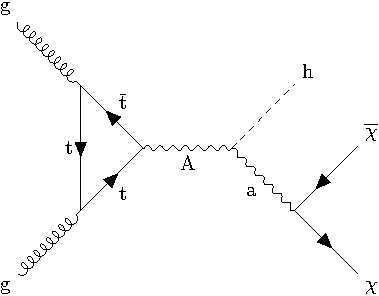
\includegraphics[width=0.4\textwidth]{figures/Feyn-2HDMa.pdf}}\hspace{1cm}
 \subfloat{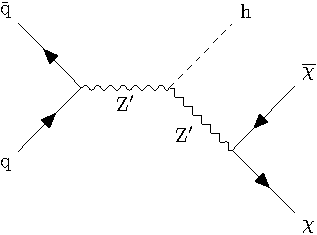
\includegraphics[width=0.34\textwidth]{figures/Feyn-Baryonic.pdf}} \\
\caption{Feynman diagrams for the 2HDM+$a$ model (left) and the baryonic Z' model (right).}
\label{feyns}
\end{figure}


%The quantity \ptvecmiss, calculated as the negative vectorial sum of the transverse momentum (\pt) of all objects identified in an event, 
%represents the total
%momentum carried by the DM particles.
%The magnitude of this vector is referred to as \MET.
%For a given value of \mzp, the \pt of the \Az decreases as its mass increases.
%Therefore, the \MET spectrum softens with increasing \Az masses.
%A comparison of the \MET distributions expected from representative scenarios of the \cPZpr-2HDM model and the \cPZpr-Baryonic model are presented in Fig.~\ref{fig:met_signals}.


%\begin{figure}
%\centering
%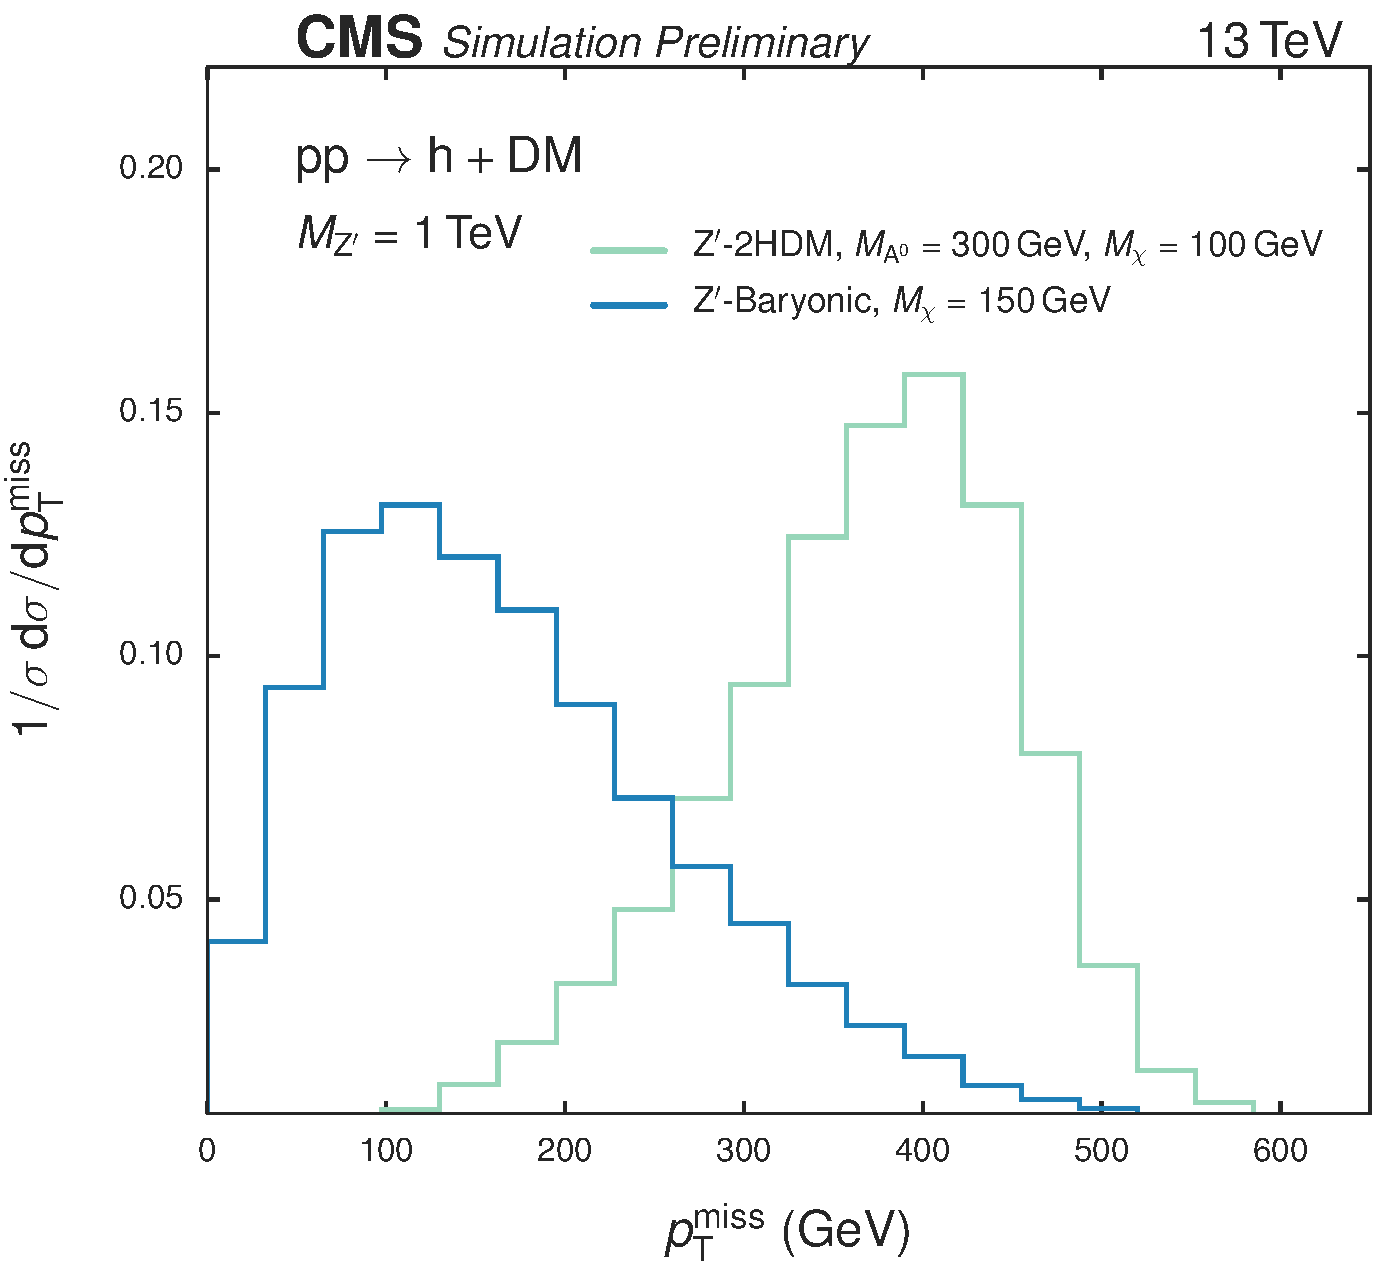
\includegraphics[width=0.55\textwidth]{figures/puppimet_signals.pdf}
%\includegraphics[width=0.45\textwidth]{figures/ZpBaryonicModel.pdf}
%\caption{Reconstructed \MET for representative scenarios of two $\mathrm{h}+\mathrm{DM}$ models investigated. Coupling parameters are chosen as mentioned in the text. The \cPZpr-2HDM model in general has a significant harder \MET~spectrum than the \cPZpr-Baryonic model, which makes the former easier to distinguish from SM background processes.}
%\label{fig:met_signals}
%\end{figure}

Signal events are characterized by a large imbalance in the transverse
momentum (or hadronic recoil), which indicates the presence of invisible
DM particles, and by hadronic activity consistent with the production
of an SM Higgs boson that decays into a $b\bar{b}$ pair. Thus, our search
strategy is to impose requirements on the mass of the reconstructed
Higgs boson candidate, together with the identification of the
products of hadronization of the two b quarks produced in the Higgs
boson decay, to define a data sample that is expected to be enriched
in signal events. Several different SM processes can mimic this topology, such as top quark pair production and the production of a vector boson (V) in association with multiple jets. Statistically independent data samples are used to predict the hadronic recoil distribution for these SM processes that constitute the largest sources of background.
Both signal and background contributions to the data are extracted with a likelihood fit to the hadronic recoil distribution, performed simultaneously in all the different analysis subsamples.

%%===============================================================================
\section{The CMS detector, particle reconstruction, and event simulation}
\label{sec:cms}

The CMS detector, described in detail in Ref.~\cite{CMSdetector}, is a multipurpose apparatus designed to study high-transverse momentum ($\pt$) processes in proton-proton and heavy ion collisions.  
%
A superconducting solenoid occupies its central region, providing a magnetic field of 3.8\unit{T} parallel to the beam direction. 
%
Charged-particle trajectories are measured using the silicon pixel and strip trackers, which cover a pseudorapidity region of $\abs{\eta} < 2.5$. 
%
A lead tungstate (PbWO$_4$) crystal electromagnetic calorimeter (ECAL) and a brass/scintillator hadron calorimeter (HCAL) surround the tracking volume and cover $\abs{\eta} < 3$. 
%
The steel and quartz-fiber forward Cherenkov hadron calorimeter extends the coverage to $\abs{\eta} < 5$.  
%
The muon system consists of gas-ionization detectors embedded in the steel flux-return yoke outside the solenoid and covers $\abs{\eta} < 2.4$. 
%
The return yoke carries a 2\unit{T} return field from the solenoid.
%
The first level of the CMS trigger system is designed to select events in less than 4\mus, using information from the calorimeters and muon detectors. 
%
The high-level trigger-processor farm then reduces the event rate to several hundred Hz.
%


The particle-flow (PF) event algorithm~\cite{Sirunyan:2017ulk} aims at reconstructing and identifying each individual particle through an optimized combination of information from the different elements of the CMS detector. 
%
The energy of a photon is obtained directly from the ECAL measurement, corrected for effects from neglecting signals close to the detector noise level, termed zero-suppression in the following. 
%
The energy of an electron is determined from a combination of the electron momentum at the primary interaction vertex as determined by the tracker, the energy of the corresponding ECAL cluster, and the energy sum of all photons spatially compatible with originating from the electron track.
% 
The energy of a muon is obtained from the curvature of the corresponding track. 
%
The energy of a charged hadron is determined from a combination of its momentum measured in the tracker and the matching ECAL and HCAL energy deposits, corrected for zero-suppression effects and for the response function of the calorimeters to hadronic showers. 
%
Finally, the energy of a neutral hadron is obtained from the corresponding corrected ECAL and HCAL energy.
%

%This analysis uses pp collision data at $\sqrt{s}=13\TeV$ recorded by the CMS experiment at the LHC during 2016.
%
%The data correspond to an integrated luminosity of $35.9\,\text{fb}^{-1}$. 
%
%Control regions obtained by requiring the presence of muons or electrons are employed in the search for $\MET+\mathrm{h}(\mathrm{b}\bar{\mathrm{b}})$; therefore, the \MET and SingleElectron datasets are used for offline analysis. 
%
%The \MET dataset includes muon pass-through triggers, which allow for selecting events with high $\MET$ or high muon recoil.

\section{The CMS detector}

The CMS detector, described in detail in Ref.~\cite{CMSdetector}, is a multipurpose apparatus designed to study high-transverse momentum ($p_\mathrm{T}$) processes in proton-proton (pp) and heavy ion collisions.
%                                                                                                                                                                                                    
A superconducting solenoid occupies its central region, providing a magnetic field of 3.8\unit{T} parallel to the beam direction.
%                                                                                                                                                                                                    
Charged-particle trajectories are measured using silicon pixel and strip trackers that cover a pseudorapidity region of $\abs{\eta} < 2.5$.
%                                                                                                                                                                                                    
A lead tungstate crystal electromagnetic calorimeter (ECAL), and a brass and scintillator hadron calorimeter  surround the tracking volume and extend to $\abs{\eta} < 3$.
%                                                                                                                                                                                                    
The steel and quartz-fiber forward Cherenkov hadron calorimeter extends the coverage to $\abs{\eta} < 5$.
%                                                                                                                                                                                                    
The muon system consists of gas-ionization detectors embedded in the steel flux-return yoke outside the solenoid and covers $\abs{\eta} < 2.4$.
%                                                                                                                                                                                                    
%The return yoke carries a 2\unit{T} return field from the solenoid.
%                                                                                                                                                                                                    
Online event selection is accomplished via the two-tiered CMS trigger
system~\cite{1748-0221-12-01-P01020}. The first level is designed to select events in less than
4\mus, using information from the calorimeters and muon detectors.
%                                                                                                                                                                                                    
Subsequently, the high-level trigger processor farm reduces the event rate to 1~kHz.


\section{Simulated data samples}

The signal processes are simulated at leading order (LO) accuracy in quantum chromodynamics (QCD) perturbation theory using the \MADGRAPH{\textsc 5\_aMC@NLO} v2.4.2~\cite{amcatnlo} program.
%
To model the contributions from SM Higgs boson processes as well as
from the \ttbar and single top quark backgrounds, we use the {\sc Powheg~v2}~\cite{Nason:2004rx,Frixione:2007vw,Alioli:2010xd} generator. These processes are generated at the next-to-leading order (NLO) in QCD. The \ttbar production 
cross section is further corrected using calculations at the next-to-next-to-leading order (NNLO) in QCD including corrections for soft-gluon radiation estimated with next-to-next-to-leading logarithmic accuracy~\cite{ttbarNNLO}. 
% 
Events with multiple jets produced via the strong interaction (referred to as QCD multijet events) are generated at LO using \MADGRAPH{\textsc 5\_aMC@NLO} v2.2.2 with up to four partons in the matrix element calculations. The MLM prescription~\cite{mlm} is used for matching these partons to parton shower jets.
%
Simulated samples of Z+jets and W+jets processes are generated at LO using \MADGRAPH{\textsc 5\_aMC@NLO} v2.3.3. Up to four additional partons are considered in the matrix element and matched to their parton showers using the MLM technique.
%
The V+jets samples are corrected by weighting the \pt of the respective boson with NLO QCD corrections obtained from large samples of events generated with \MADGRAPH{\textsc 5\_aMC@NLO} and the FxFx merging technique~\cite{fxfx} with up to two additional jets stemming from the matrix element calculations.
%
These samples are further corrected by applying NLO electroweak corrections~\cite{Kuhn:2005gv,Kallweit:2015fta,Kallweit:2015dum} that depend on the boson \pt.
%
Predictions for the SM diboson production modes WW, WZ, and ZZ are obtained at LO with the {\sc \PYTHIA 8.205}~\cite{Sjostrand:2014zea} generator and normalized to NLO accuracy using {\sc mcfm v6.0}~\cite{MCFM}. 
%


The LO or NLO NNPDF 3.0 parton distribution functions (PDFs)~\cite{Ball:2014uwa} are 
used, depending on the QCD order of the generator used for each physics 
process. 
%
Parton showering, fragmentation, and hadronization are simulated with {\sc \PYTHIA 8.212} using the CUETP8M1 underlying event tune~\cite{ue1,ue2}. 
%
Interactions of the resulting final state particles with the CMS detector are simulated using the \GEANTfour program~\cite{geant4}.
%
Additional inelastic pp interactions in the same or a neighboring bunch crossing (pileup) are included in the simulation.
%
The pileup distribution is adjusted to match the corresponding distribution observed in data. 


%A global event reconstruction is performed using the particle-flow (PF) \cite{CMS-PAS-PFT-09-001, ParticleFlow} algorithm.
%, which optimally combines the information from all subdetectors and 
%produces a list of stable particles (muons, electrons, photons, 
%charged and neutral hadrons). 


\section{Event reconstruction}

The reconstructed interaction vertex with the largest value of $\sum_{i} p_\mathrm{T}^{i2}$, where $p_\mathrm{T}^{i}$ is the transverse momentum of the $i^\mathrm{th}$ track 
associated with the vertex, is selected as the primary event vertex. The offline selection requires all events to have at least one primary vertex reconstructed within a 24\,cm window along the z-axis around the nominal interaction point, and a transverse distance from the nominal interaction region less than 2\,cm.

The particle-flow (PF) \cite{Sirunyan:2017ulk} algorithm aims to reconstruct all the physics objects described in this section. At large Lorentz boosts, the two b quarks from the Higgs boson decay may produce jets that overlap and make their individual reconstruction difficult. In this search, large-area jets clustered from PF candidates using the Cambridge--Aachen algorithm~\cite{cajets} with a distance parameter of $1.5$ (CA15 jets) are utilized to identify the Higgs boson candidate.  The large cone size is chosen in order to include events characterized by the presence of Higgs bosons with medium boost ($p_\mathrm{T}$ of the order of 200 GeV).
To reduce the impact of particles arising from pileup interactions,  the four-vector of each PF candidate is scaled with a weight calculated with the pileup per particle identification (PUPPI) algorithm ~\cite{puppi} prior to the clustering.
The absolute jet energy scale is corrected using calibrations derived from data~\cite{jec}. The CA15 jets are also required to be central ($\eta$ $<$ 2.4).
The ``soft-drop'' (SM) jet grooming algorithm~\cite{msd} is applied to remove soft wide-angle radiation from the jets. We refer to the groomed mass of the CA15 jet as $m_\text{SD}$. 

The ability to identify two b quarks inside a single CA15 jet is
crucial for this search. A likelihood for the CA15 jet to contain two
b quarks is derived by combining the information from primary and secondary vertices and tracks in a multivariate discriminant optimized to distinguish the Higgs to \bb decays from energetic quarks or gluons~\cite{Sirunyan:2017ezt} that appear inside the CA15 jet cone.
%The chosen working point of double b-tagger ($>$ 0.75) corresponds to the same background efficiency of the medium 
%working point of minimum of the CSV score of subjets. 
The working point chosen for this algorithm (the ``double-b tagger'')
corresponds to an identification efficiency of 50\% for a \bb system
with a \pt of 200 GeV, and a probability of about 10-13\% for
misidentifying CA15 jets originating from other combinations of quarks
or gluons. The efficiency of the algorithm increases with the \pt~of the \bb system.

%These numbers have been determined in simulation samples with at least one reconstructed CA15 jet with $\pt>200$\GeV and an otherwise inclusive selection. 

Energy correlation functions are used to identify the two-prong
structure in the CA15 jet expected from a Higgs boson decay to two b
quarks. The energy correlation functions are sensitive to correlations among the constituents
of CA15 jets (the PF candidates)~\cite{ecf}. They are $N$-point correlation functions ($e_N$) of the constituents' momenta, weighted by the angular separation of the constituents.
%Discriminating variables are constructed by using ratios of these functions.
%\begin{linenomath}
%\begin{equation}
%  \frac{_ae_N^\alpha}{(_be_M^\beta)^x}, \text{ where $M\leq N$ and $x= \frac{a\alpha}{b\beta}$}.
%  \label{eq:ecf}
%\end{equation}
%\end{linenomath}
%                                                                                                                                                                                                
%In Eq.~(\ref{eq:ecf}), the six free parameters are
%$N,a,\alpha,M,b,~\mathrm{and}~\beta$ and the value of $x$ is chosen to
%make the ratio dimensionless. An $N$-pronged jet is expected to have
%$e_N \gg e_M$ for $M>N$. 
As motivated in Ref.~\cite{ecf}, the ratio $N_2 =
e_3^{(\beta)}/(e_2^{(\beta)})^2$ is proposed as a two-prong tagger for
the identification of the CA15 jet containing the Higgs boson decay
products; the parameter $\beta$, which controls the weighting of the angles between constituent pairs in the computation of
the $N_2$ variable, is chosen to be 1 as the value that gives the best two-prong jet reconstruction. 

%\begin{equation}
%  N_2(\beta) = \frac{e(2,3,\beta)}{e(1,2,\beta)^2}
%\end{equation}

%When computing the $N_2$ variable, only the first one hundred highest $p_T$ constituents that survive soft-drop grooming are used.

It is noted that requiring a jet to be two-pronged by using a jet substructure variable,
such as $N_2$, will affect the shape of the distribution of $m_\text{SD}$ for the
background processes. In this search, the value of $m_\text{SD}$ is required to be consistent with the Higgs boson mass.
It is therefore desirable to preserve a smoothly falling jet mass
distribution as a function of \pt as the one expected for QCD-like jets (i.e., jets that
do not originate from a heavy resonance decay). 
As motivated in Ref.~\cite{ddt}, the stability of $N_2$ is tested against the variable
$\rho=\ln(m_{\text{SD}}^2/\pt^2)$, since the distribution of $\rho$ is expected to be stable in QCD-like jets.
%: since the jet mass distribution for QCD multijet
%events is expected to scale with \pt, decorrelating the $N_2$ variable
%as a function of $\rho$ and \pt would be the most appropriate procedure. 
The decorrelation strategy described in Ref.~\cite{ddt} is applied,
choosing a background efficiency of 20\%, which corresponds to a
signal efficiency of roughly 50\%. This results in a modified tagging
variable, which we denote as $N_2^\text{DDT}$, where the superscrit DDT stands for designing decorrelated taggers~\cite{ddt}. Fig.~\ref{n2ddt} shows the expected distribution of the the $N_2^\text{DDT}$ for CA15 jets matched to a Higgs boson decaying to a $b\bar{b}$ pair, together with the distributions expected for CA15 jets matched to hadronically decaying top quarks and for QCD-like CA15 jets.
%This choice of background (or, equivalently, signal) efficiency has been optimized in order to maximize the $S/B$ ratio while retaining high enough event yield for the data-driven estimation of the background processes.
\begin{figure}
\centering
  \includegraphics[width=0.65\textwidth]{figures/ddt_N2DDT_ns.pdf} \\
\caption{The $N_2^\text{DDT}$ distribution as expected for CA15 jets matched to a Higgs boson decaying to a $b\bar{b}$ pair (in red), compared to the expected distribution for CA15 matched to the decay products of top quarks decaying hadronically (in grey). The distribution corresponding to CA15 jets that do not originate from a heavy resonance decay is also shown in blue.}
\label{n2ddt}
\end{figure}


This search also utilizes narrow jets clustered
with the anti-$\kt$ algorithm~\cite{Cacciari:2008gp}, with a distance
parameter of $0.4$ (“AK4” jets). Narrow jets originating from b quarks are identified using the combined secondary vertex (CSVv2) algorithm \cite{Sirunyan:2017ezt}. The working point used in this search has a b jet identification efficiency of 81\%, a charm jet selection efficiency of 37\%, and a 9\% probability of misidentifying light-flavor jets~\cite{Sirunyan:2017ezt}. Jets that are b tagged are required to be central ($|\eta|<2.4$).
%%An event with any additional narrow jet passing the loose b tagging requirement is vetoed to reduce the number of events containing top quarks. 

Electron reconstruction requires the matching of a supercluster in the ECAL with a track in the silicon tracker.
Identification criteria~\cite{Khachatryan:2015hwa} based on the ECAL shower shape and the consistency with originating from the primary vertex are imposed. The reconstructed electron is required to be within $|\eta|< 2.5$, excluding the transition region $1.44<|\eta|<1.57$ between the ECAL barrel and endcap. Muons candidates are selected by two different reconstruction approaches~\cite{CMSMuonJINST}: the one in which tracks in the silicon tracker are matched to a track
 segment in the muon detector, and the other one in which a track
 fit spanning the silicon tracker and muon detector is performed
 starting with track segments in the muon detector. Candidates that are found by both the approaches are considered as single candidates.
Further identification criteria are imposed on muon candidates to reduce the number of misidentified hadrons and poorly measured mesons tagged as muons~\cite{CMSMuonJINST}. 
These additional criteria include requirements on the number of hits in the tracker and in the muon systems, the fit quality of the global muon track, and its consistency with the primary vertex.
Muon candidates with $|\eta|< 2.4$ are considered in this analysis. 
With electron and muon candidates, the minimum \pt is required to be 10\GeV. Isolation is required for both the objects.
Hadronically decaying $\tau$ leptons, $\tau_\mathrm{h}$, are reconstructed using the hadron-plus-strips
  algorithm~\cite{CMSTauJINST}, which uses the charged hadron and neutral electromagnetic objects 
to reconstruct intermediate resonances into which the $\tau$ lepton decays. The $\tau_\mathrm{h}$
candidates with $\pt>18\GeV$ and $|\eta|< 2.3$ are considered~\cite{Khachatryan:2015hwa,Chatrchyan:2013sba,CMSTauJINST}. Photon candidates, identified by means of requirements on the ECAL energy distribution and its distance to the closest track, must have $\pt>15\GeV$ and $|\eta|< 2.5$. %We veto both $\tau_\mathrm{h}$ candidates and photon candidates in the search presented. %Events containing an isolated electron, muon, or an isolated hadronic tau passing these criteria are 

The missing transverse momentum $\vec{p}_{\mathrm{T}}^{\mathrm{miss}}$ is defined as the negative vectorial sum of the \pt of all the reconstructed PF candidates. Its magnitude is denoted as \MET. Corrections to jet momenta are propagated to the \MET calculation as well as event filters \cite{CMS-PAS-JME-16-004} are used to remove spurious high \MET events caused by instrumental noise in the calorimeters or beam halo muons~\cite{CMS-PAS-JME-16-004}. The filters remove about 1\% of signal events.

%For the control regions involving lepton(s) in the final state, the hadronic recoil against the boson is computed by removing the \pt of the lepton(s) from the \MET computation. The recoil is given by: 
%\begin{equation} 
%\vec{U}  = \MET + p_{\mathrm{T}}^{\ell,\ell\ell} 
%\end{equation} 
%where the \pt$^{l}$ is \pt of lepton(s) in the W (Z) control regions. 

\section{Event selection}


Signal events are characterized by a high value of \MET, no isolated leptons or photons, and a CA15 jet identified as a Higgs boson candidate. In the signal region (SR) described
below, the dominant background contributions arise from Z+jets,
W+jets, and \ttbar production. To predict the \ptmiss~spectra of these
processes in the SR, data from different control regions (CRs) are used. Single-lepton CRs are designed to predict the \ttbar and W+jets backgrounds, while dilepton CRs predict the Z+jets background contribution. The hadronic recoil, $U$, defined by removing the \pt of the lepton(s) from the \MET computation in CRs, is used as a proxy for the \MET distribution of the main background processes in the SR. Predictions for other backgrounds are obtained from simulation.

A common set of preselection criteria is used for all regions. The presence of exactly one CA15 jet with $\pt>200\GeV$ and $|\eta|<2.4$ is required. It is also required that $100<m_{\text{SD}}<150\GeV$ and $N_2^{\text{DDT}}<0$. This minimizes extrapolation uncertainties when deriving a prediction for the SM backgrounds in the SR by means of the CRs, as the CA15 jet is ensured to have the same flavor content for a given process across all regions.
 In the SR (CRs), \ptmiss~($U$) has to be larger than 200\GeV, and the minimum distance in the azimuthal angle $\phi$ between any AK4 jet and the direction of \ptmiss ($U$) must be larger than 0.4 to reject multijet events that mimic signal events. Vetoes on $\tau_\text{h}$ candidates and photon candidates are applied, and the number of AK4 jets that do not overlap with the CA15 jet must be smaller than two. This significantly reduces the contribution from \ttbar events.

\begin{table}\footnotesize
  \begin{center}
  \caption{Event selection criteria defining the signal regions and control regions. These criteria are applied in addition to the preselection that is common to all regions, 
as described in the text. } \label{tab:event_selection}
    \begin{tabular}{  l | c | c | c | c }
      \hline \hline
        Region   & Main processes & Additional AK4 b tag   & Leptons & Double-b tag \\ \hline
        Signal   & Z+jets, \ttbar, W+jets & 0                & 0       & pass \\ \hline
        Single-lepton, b-tagged   &  \ttbar, W+jets & 1                & 1       & pass/fail\\ \hline
        Single-lepton, anti-b-tagged        & W+jets, \ttbar & 0                & 1       & pass/fail\\ \hline
        Dilepton & Z+jets & 0                & 2       & pass/fail\\
      \hline \hline
    \end{tabular}
  \end{center}
\end{table}


Events that meet the preselection criteria described above are split into the SR and the different CRs based on their lepton multiplicity and the presence of a b-tagged AK4 jet not overlapping with the CA15 jet, as summarized in Table~\ref{tab:event_selection}. For the SR, events are selected if they have no isolated muons (electrons) with $\pt >10\GeV$ and $|\eta|< 2.4$ (2.5). The previously described double-b tag requirement on the Higgs boson candidate CA15 jet is imposed.
Events are selected online by requiring large values of $p_\text{T,trig}^\text{miss}$ or $H_{\text{T}}^{\text{miss}}$ (between 90 and 120\GeV, depending on the data-taking period), where $p_\text{T,trig}^\text{miss}$  ($H_{\text{T}}^{\text{miss}}$) is the magnitude of the vectorial sum of $\vec{p}_\text{T}$ of all the particles (jets with $\pt>20\GeV$) at the trigger level. Muon candidates are excluded from the online $p_\text{T,trig}^\text{miss}$ calculation.

%The single- or dielectron CRs are populated with events selected by requiring high-\pt electrons.



%hresholds imposed online on the electron \pt vary from 25\,GeV to 105\,GeV depending on the identification and isolation criteria.  

%The different CRs defined in Table~\ref{tab:event_selection} are used to control the three main background processes.  Since the hadronic recoil $U$ is computed removing the muon(s) or the electron(s) from the \MET calculation, its distribution can be used as a proxy to model the \MET distribution in the SR. 
%Both the normalization and the shape of the \ttbar, Z+jets, and W+jets background processes are constrained by transfer factors from the CRs to the SR estimated in bins of $U$. These transfer factors correlate the same bins across all regions and are allowed to vary within uncertainties.% as described in Section~\ref{sec:systematics}.
To predict the \MET spectrum of the Z+jets process in the SR, dimuon and dielectron CRs are used.
Dimuon events are selected online employing the same \MET triggers that are used in the SR.
These events are required to have two oppositely charged muons (having
\pt $>$ $20\GeV$ and \pt $>$ $10\GeV$ for the leading and trailing
muon, respectively), with an invariant mass between 60\GeV and 120\GeV.
The leading muon has to satisfy tight identification and isolation requirements that result in an efficiency of 95\%.
Dielectron events are selected online using single-electron triggers. %, which have a \pt threshold of $27\GeV$.
Two oppositely charged electrons with \pt greater than $10\GeV$ are required offline, and they must form an invariant mass between 60\GeV and 120\GeV.
To be on the plateau of the trigger efficiency, at least one of the two electrons must have $\pt>40\GeV$, and it has to satisfy tight identification and isolation requirements that correspond to an efficiency of 70\%.

Events that satisfy the SR selection due to the loss of a single lepton primarily originate from W+jets and semileptonic \ttbar events.
To predict these backgrounds, four single-lepton samples are used: single-muon and single-electron, with or without a b-tagged AK4 jet outside the CA15 jet.
The single-lepton CRs with a b-tagged AK4 jet target \ttbar events, while the anti-b-tagged single-lepton CRs target W+jets events.
Single muon events are selected using the \MET trigger.
The electron (muon) candidate in these events is required to have \pt $>$ 40\GeV (20\GeV) and has to satisfy tight identification and isolation requirements.
In addition, samples with a single electron need to have $\ptmiss>50\GeV$ to avoid a large contamination with multijet events.

%With the exception of b tagging, all other selection requirements used for signal events are imposed, using $U$ instead of \ptmiss.
%In the anti-b-tagged single muon CR, the b tagging requirement is reversed.

Each CR is split into two subsamples depending on whether or
not they satisfy the double-b tag requirement imposed to define the SR. This allows for an in situ calibration of the scale factor that corrects the misidentification probability of the double-b tagger for the three main backgrounds obtained from simulation to the one observed in data. 

\section{Signal extraction}

As mentioned in Section~\ref{intro}, signal and background contributions to the data are extracted with a simultaneous binned likelihood fit (using the ROOStat package~\cite{roostats}) to the \MET and $U$ distributions in the SR and the CRs.
%
The dominant SM process in each CR is used to predict the respective background in the SR via transfer factors $T$. They are determined in simulation and are given by the ratio of the prediction for \ptmiss in the SR and the $U$ prediction in the CR for the given process. This ratio is determined independently for each bin of the corresponding distribution.
  
For example, if $b\ell$ denotes the \ttbar~process in the b-tagged single-lepton control sample that is used to estimate the \ttbar contribution in the SR, the expected number of \ttbar events, $N_{i}$, in the $i^\text{th}$ bin of the SR is then given by $N_{i}= \mu^{\ttbar}_{i}/T^{b\ell}_{i}$, where  $\mu^{\ttbar}_i$ is a freely floating parameter included in the likelihood to scale the \ttbar contribution in bin $i$ of $U$ in the CR.

The transfer factors used to predict the W+jets and the \ttbar background take into account the impact of lepton acceptances and efficiencies, the b tagging efficiency, and, for the single-electron control samples, the additional requirement on \MET.
%This transfer factor explicitly includes hadronic tau leptons that fail the hadronic tau lepton identification criteria, which account for roughly 20-80\% of the total W+jets background in the high recoil region.  differences in \ptmiss trigger efficiencies observed between single-muon and dimuon events,
Since the anti-b-tagged CR with a double-b tag also has a significant contribution from the \ttbar process,  transfer factors to constrain \ttbar are also imposed between the b-tagged and anti-b-tagged single-lepton CRs.
%This allows for an estimation of the \ttbar contribution in the signal region to be made from W+jets CRs to be made from the b-tagged CR. 
A similar constraint is imposed to estimate the contamination from W+jets production in the \ttbar CR with events that fail the double-b tag requirement. 
Likewise, the Z+jets background prediction in the signal region is connected to the dimuon and dielectron CRs through transfer factors.
They account for the difference in the branching fractions of $\mathrm{Z}\rightarrow \nu\nu$~and $\mathrm{Z}\rightarrow \ell\ell$ decays and the impacts of lepton acceptances and selection efficiencies.


.\section{Systematic uncertainties}

 Nuisance parameters are introduced into the likelihood fit to represent the systematic uncertainties of the search. They can either affect the rate or  the shape of \ptmiss ($U$) for a given process in the SR (CRs) and can be constrained in the fit. Shape uncertainties are incorporated by means of a prior Gaussian distribution, while rate uncertainties are given a prior log-normal distribution. A summary of systematic uncertainties is presented in Table~\ref{tab:systs}.


\begin{table}\footnotesize
\begin{center}
  \caption{Systematic uncertainties, along with the type (rate/shape) of uncertainty and the affected processes. For the rate uncertainties, the percentage effect on the rate is quoted.}
\begin{tabular}{l r r}
  \hline\hline
Systematic uncertainty & Type & Processes \\
\hline
double-b tagging & shape & Z+jets, W+jets, \ttbar, SM h, signal\\
heavy flavor fraction & 4-5\% & Z+jets, W+jets\\
\ptmiss~trigger efficiency & 1\% & all \\
single-electron trigger & 1\% & all \\
lepton efficiency & 1\% per leg & all \\
$\tau$ lepton veto & 3\% & all \\
%AK4 b tagging & shape & all \\
\ptmiss~trigger muon multiplicity & shape & Z+jets, W+jets \\
theoretical cross section & 20\% & t, diboson\\
multijet normalization & 100\% & multijet \\
\ptmiss magnitude & 5\% & all \\
CA15 jet energy & 4\% & t, diboson, multijet, SM h, signal \\
$N_2^\text{DDT}$ efficiency & 7\% & diboson, SM h, signal \\
luminosity & 2.5\% & t, diboson, multijet, SM h, signal \\
bin-by-bin statistics & shape & \ttbar, Z+jets, W+jets \\
\hline\hline
  \end{tabular}
\label{tab:systs}
\end{center}
\end{table}

Scale factors are used to correct for differences in the double-b tagger misidentification efficiencies between data and prediction from simulation for W/Z+jets production and for \ttbar production. These scale factors affect only the overall rates of the respective processes, and they are measured directly in the fit by simultaneously fitting events that pass or fail the double-b tag requirement. The uncertainties on the scale factor measurements are the one with the largest impact on the measurement.

To take into account the variation of the double-b tagging efficiency
introduced by the uncertainty in the heavy flavor fraction of W/Z+jets
events, the efficiencies are reevaluated after varying the heavy
flavor component in the simulation. The difference in the efficiency with respect to the nominal efficiency value is taken as a systematic uncertainty.

%
The correlation between the double-b tagger and the \ptmiss (or $U$) introduces a shape uncertainty in the transfer factors from the CRs with events that satisfy the inverted double-b tag criterion. This shape uncertainty is anchored at the first bin where the magnitude of the uncertainty is 0\%, and increases to 8\% in the last hadronic recoil bin. These numbers are extrapolated reflecting the level of correlation between the tagger and the \ptmiss/$U$, estimated by fitting the profile of the two-dimensional distribution double-b-vs-\ptmiss/$U$.
%

For the signal and the SM h processes, an uncertainty in the double-b tagging efficiency is applied that is 3\% for a CA15 jet with $\pt<350\GeV$, 4\% for the intermediate \pt~regime, and 8\% for $\pt>800$\GeV. These numbers have been derived through a measurement performed in a sample enriched in multijet events with double-muon-tagged $\text{g}\to\text{b}\bar{\text{b}}$ splittings. 

An uncertainty of $21\%$ in the heavy flavor fraction of
W+jets is reported in previous CMS measurements~\cite{Khachatryan:2014uva,Chatrchyan:2013uza}. Similarly, the uncertainty on the Z+heavy flavor fraction is measured to be $22\%$~\cite{Khachatryan:2014zya,Chatrchyan:2014dha}. Depending on the b tagging requirement, the uncertainty on the heavy flavor fraction on such processes determines an uncertainty on the overall rate (the sum of heavy and light flavor components) for both W and Z+jets. To account for this effect, a flat $4\%$ is assigned to the W+jets process, while a flat $5\%$ is assigned to the Z+jets process. They are included as rate uncertainties, correlated across all regions defined by the same b tagging requirement and anti-correleted across all regions defined by inverting it.

The \ptmiss trigger efficiency is parametrized as a function of $p_\text{T,trig}^\text{miss}$. The uncertainty in its measurement is a flat 1\% and is included in the fit as a rate uncertainty.
The efficiencies of the single-electron triggers are parametrized as a
function of the electron \pt and an associated flat 1\% systematic uncertainty is added into the fit.

Uncertainties in the selection efficiencies per selected muon or electron amount to $1\%$, while the uncertainty in the $\tau$ lepton veto is $3\%$; these rate uncertainties are correlated across all $U$ bins.

The transfer factors are affected by uncertainties in the efficiencies
of lepton identification.  For example, differences on the order of
2\% in \MET trigger efficiencies are observed between single-muon and
dimuon events at lower $U$ values and represent an additional
systematic uncertainty in the transfer factors of the single-muon and
dimuon CRs. As these uncertainties depend on the momentum of the
identified lepton they can change the shape of the $U$ distribution
and are thus treated as shape uncertainties.

A systematic uncertainty of $20\%$ is assigned to the single top quark background yields~\cite{Chatrchyan:1642680} and is correlated between the SR and the CRs. 
%
An uncertainty of $20\%$ is also assigned to the diboson production cross section~\cite{Khachatryan:2016txa,Khachatryan:2016tgp} and correlated across the SR and CRs.
%

Being a negligible background source, a conservative uncertainty of $100\%$ is assigned to the QCD multijet yield. 
%
This uncertainty is estimated using a sample enriched in multijet events. The sample is obtained by vetoing leptons and photons, by requiring $\ptmiss>250$\GeV, and that the minimum azimuthal angle between $\vec{p}_{\mathrm{T}}^{\mathrm{miss}}$ and the jet directions to be less than $0.1$\,rad.
One nuisance parameter represents the uncertainty in QCD multijet yields in the signal region, while separate nuisance parameters are introduced for the muon CRs and for electron CRs.

A flat 5\% rate uncertainty in \ptmiss is obtained following the standard CMS method~\cite{Khachatryan:2014gga} and is assigned to each processes estimated from simulation.

Similarly, a flat 4\% rate uncertainty due to the imperfect knowledge of the CA15 jet energy scale~\cite{jec} is assiged to the backgrounds obtained from simulation.

A 7\% rate uncertainty in the efficiency of the the substructure variable
$N_2^\text{DDT}$ to identify two-prong CA15 jets is assigned to all processes where the decay of a resonance inside the CA15 jet cone is expected. Such processes include signal production together with SM h and diboson production.  
The uncertainty has been derived from the efficiency measurement obtained by performing a fit in a control sample
enriched in semi-leptonic \ttbar events, where the CA15 jet originates
from the W boson that comes from the hadronically decaying top quark. 
%

A rate uncertainty of 2.5\% in the luminosity measurement~\cite{CMS-PAS-LUM-17-001} is included and assigned to processes determined from simulation. In these cases, appropriate QCD scale and PDF uncertainties are also applied.
%

Nuisance parameters corresponding to bin-by-bin statistical uncertainties on the transfer factors are considered for all the processes predicted with data in CRs. 
%

Due to the similarity of selection requirements between the SR and CRs, uncertainties in the higher order NLO or EW corrections, or in the PDF, cancel out when building the ratio of yields predicted in the SR and the corresponding CR.

%Unlike the uncertainties described above, uncertainties on the signal predictions from QCD scale and PDF variations are not propagated as nuisance parameters. Instead, they are treated as uncertainties in the inclusive signal cross section. Due to the imperfect knowledge of PDFs at higher $x$, where $x$ is the momentum fraction carried by the partons participating in the hard interaction, the uncertainties increase with the mass of the final state and range from 4\% to 20\%.


\section{Results}

The expected yields for each background in the SR and their uncertainties, as determined in the likelihood fit under the background-only assumption, are presented in Table~\ref{tab:eventYieldTable}, along with the observed data yields.
%The signal region data have been included in the likelihood fit.  Table~\ref{tab:eventYieldTable_masked} lists the yields for a fit masking the data in the signal region.
Good agreement is observed between data and the predictions. Due to anticorrelations between background processes, in some bins the uncertainty in the background sum is smaller than the one in the individual contributions, such as, for example, the Z+jets yields. Expected yields are also presented for two signal models. The selection efficiencies for the chosen points correspond to 5\% for the 2HDM+$a$ model and 1\% for the baryonic Z' model. %As expected from the branching ratio of the Z boson, the uncertainties in the yields for the Z+jets process are smaller for the case where the signal region data has been included in the fit.


Figure \ref{Fig_sr} shows the pre-fit and post-fit \MET distribution in the SR for signal and for all SM backgrounds, as well as the observed data distribution. The likelihood fit has been performed simultaneously in all analysis regions. The data agree with the background predictions at the one standard deviation level, and the post-fit estimate of the SM background is slightly larger than the pre-fit one. The distributions for $U$ in the muon and electron CRs, after a fit to the data, are presented in Figs.~\ref{Fig_cr_2} and \ref{Fig_cr_1}.

\begin{figure}
\centering
 \subfloat{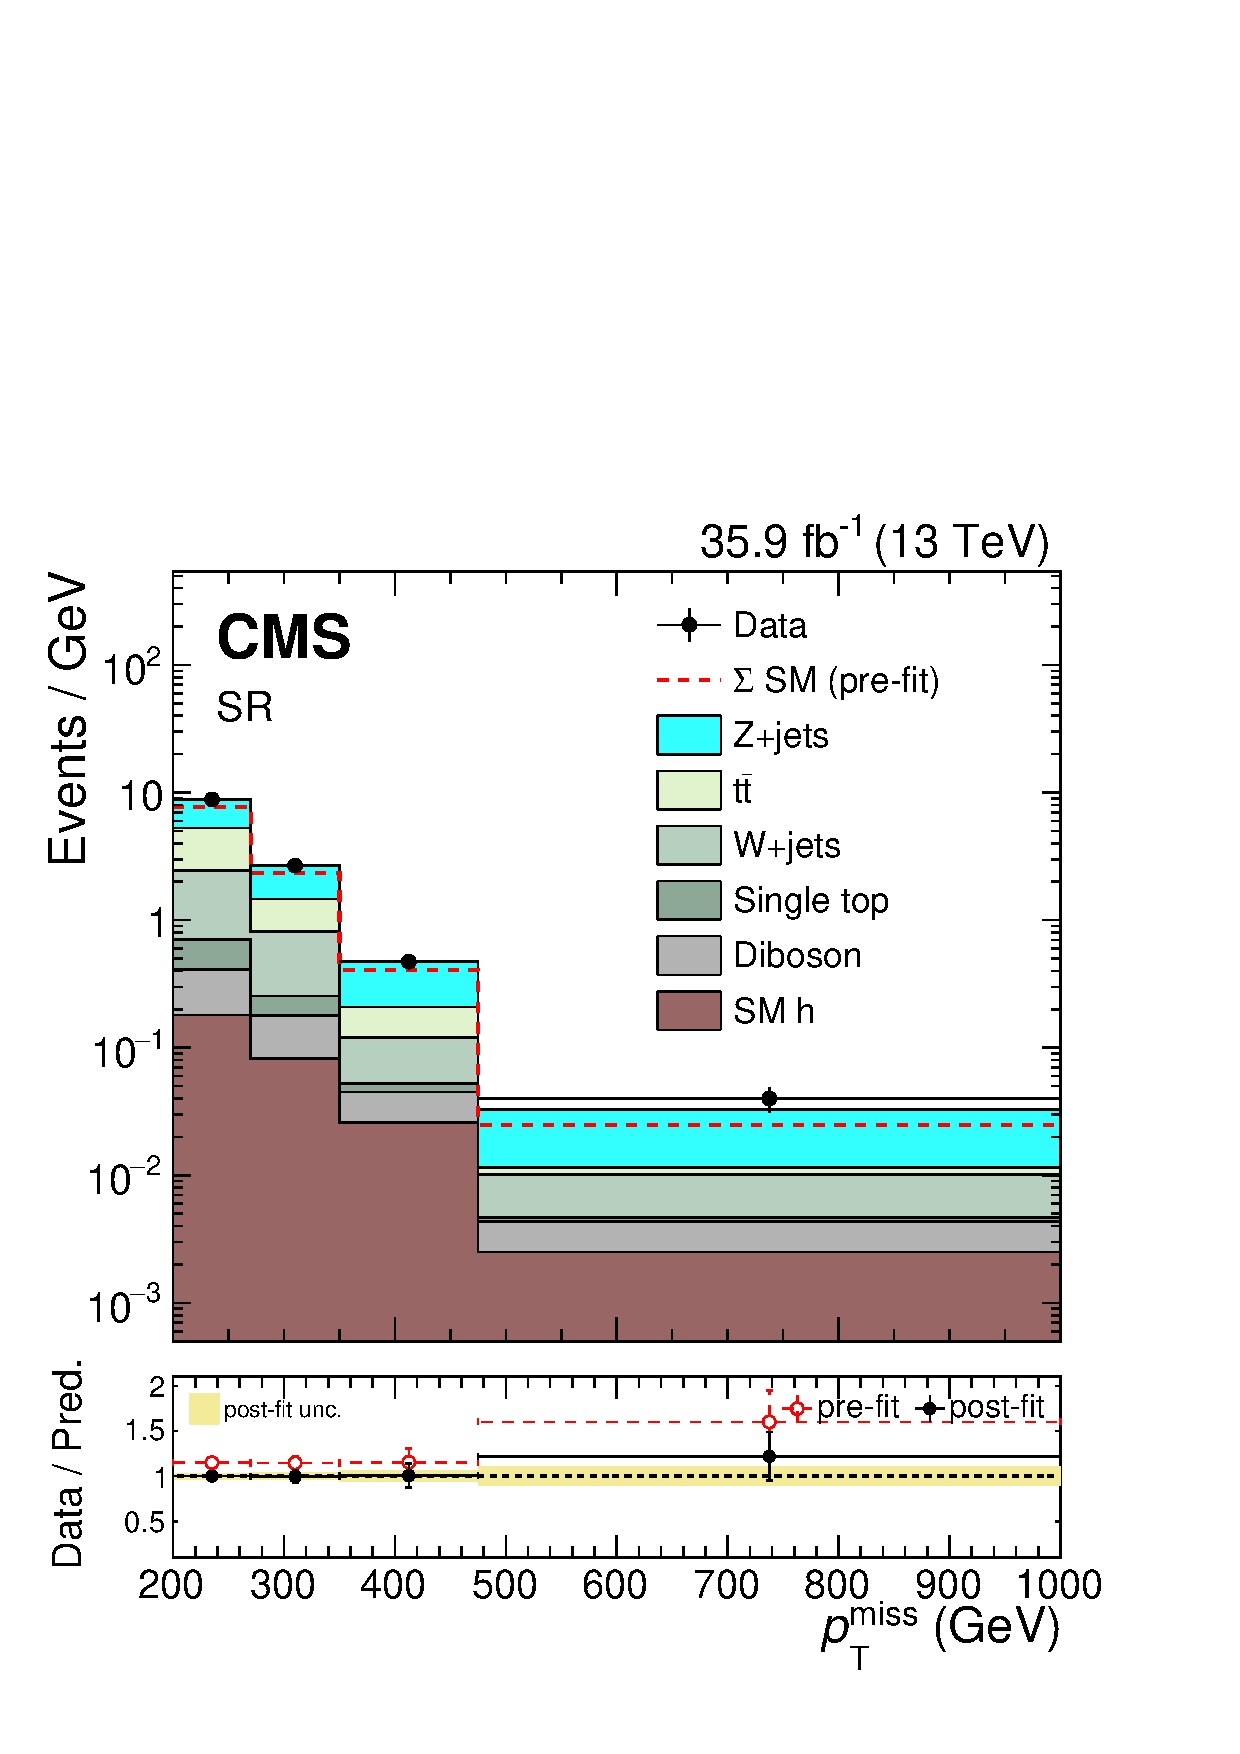
\includegraphics[width=0.45\textwidth]{figures/limits/MSDcorr_stackedPostfit_signal.pdf}}
% \subfloat{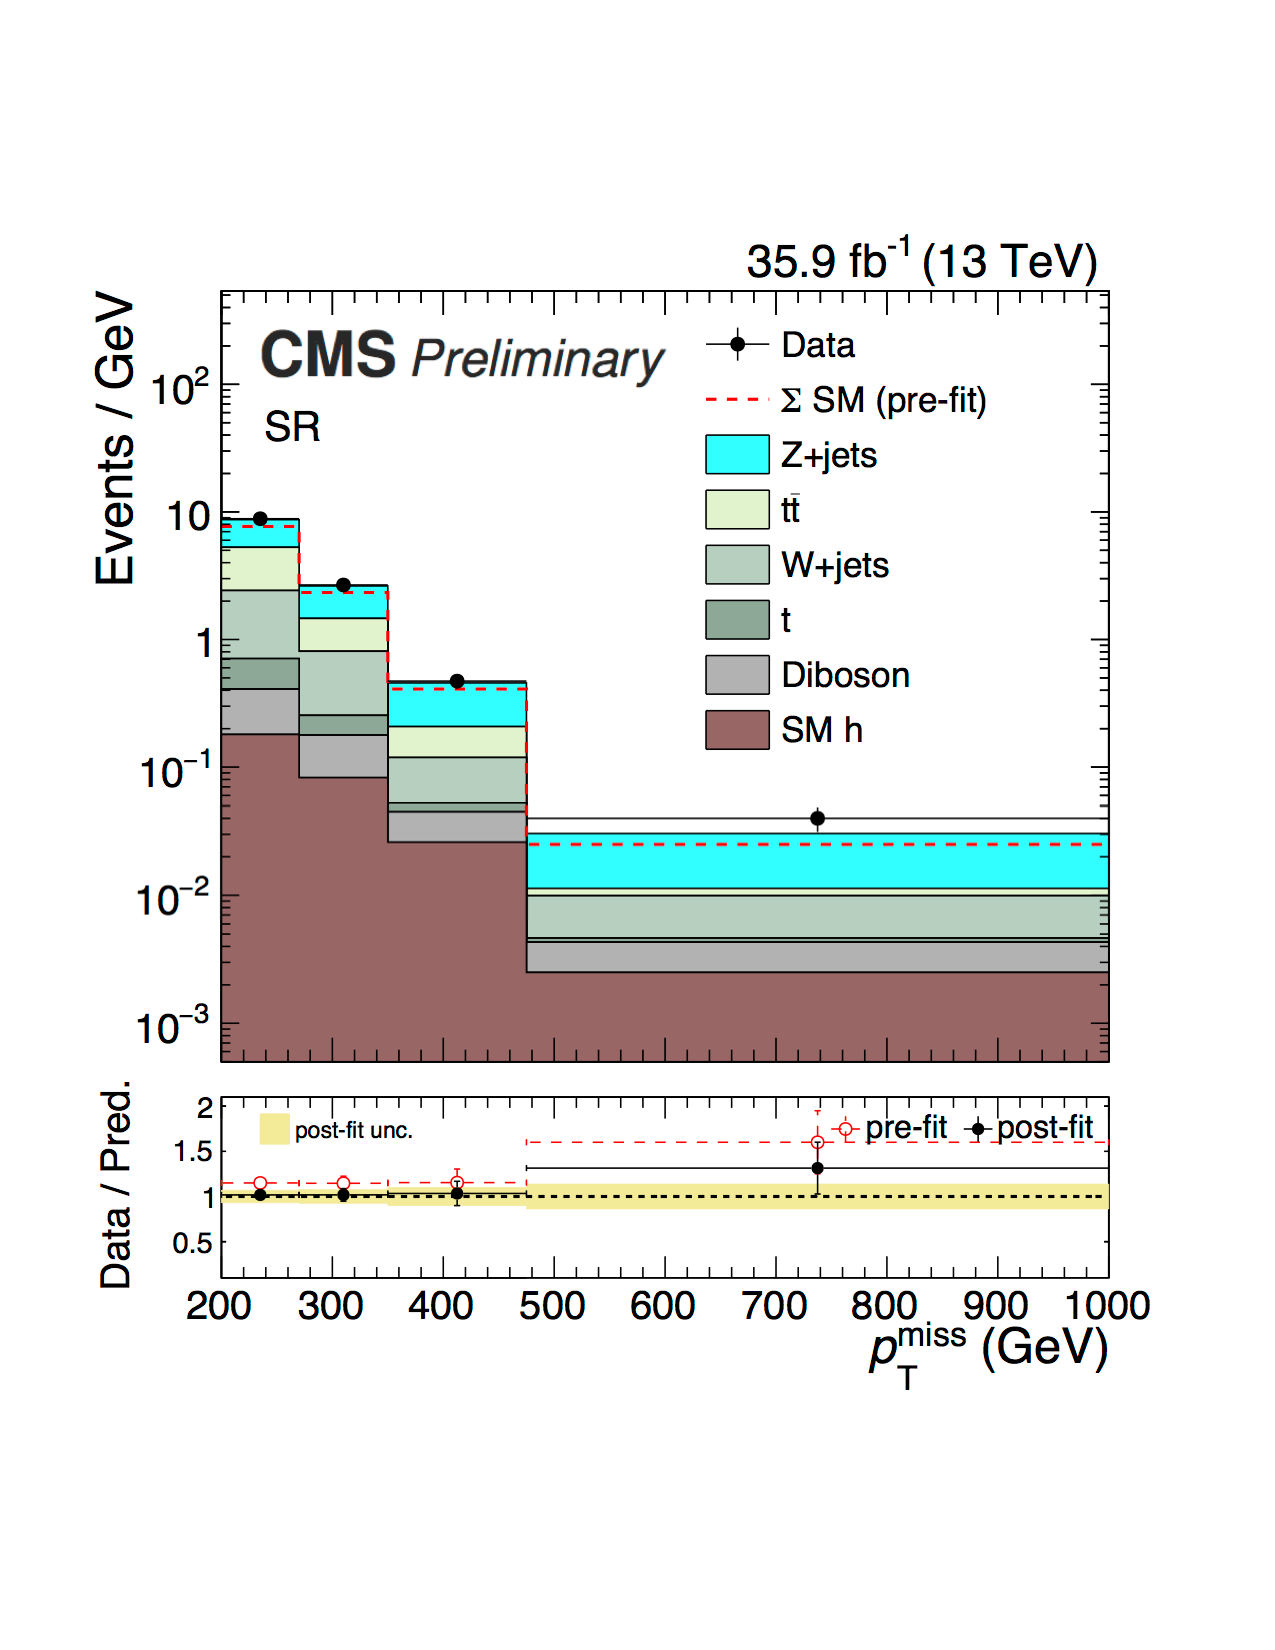
\includegraphics[width=0.45\textwidth]{figures/limits/MSDcorr_stackedPostfit_signal_masked.pdf}} \\
\caption{The \MET distribution in the signal region before and after a likelihood fit. The data are in agreement with post-fit background predictions for the SM backgrounds, and no significant excess is observed. The dashed red histogram corresponds to the pre-fit estimate for the SM backgrounds.}
\label{Fig_sr}
\end{figure}

\begin{table}\footnotesize
\begin{center}
  \caption{Post-fit event yield expectations per \ptmiss bin for the SM backgrounds in the signal region when including the signal region data in the likelihood fit, under the background-only assumption. Quoted are also the expected yields for two signal models. Uncertainties quoted in the predictions include both the systematic and statistical components.}
\\  
\begin{tabular}{l r r r r}
  \hline\hline
\ptmiss-bin         & 200-270\,GeV          & 270-350\,GeV          & 350-475\,GeV          & $>475$\,GeV         \\
\hline
Z+jets          &$ 249\pm22 $       & $97.2\pm8.5$         & $32.6\pm3.6$          & $11.1\pm1.9$       \\
\ttbar          &$ 199\pm14 $       & $52.1\pm5.2$          & $11.1\pm2.0$          & $0.7\pm0.4$        \\
W+jets          &$ 122\pm22 $       & $45.0\pm8.7$          & $8.4\pm1.9$           & $2.9\pm0.9$            \\
Single top quark      &$21.0\pm4.2 $          & $6.1\pm1.2$           & $0.9\pm0.2$           & $0.2\pm0.1$         \\
Diboson         &$ 16.0\pm3.1  $        & $7.6\pm1.5$           & $2.4\pm0.5$           & $1.0\pm0.2$ \\
SM h             &$ 12.6\pm1.4 $      & $ 6.6\pm0.7$           & $ 3.3 \pm 0.3$        & $ 1.3\pm 0.1$      \\
\hline
$\Sigma~(\text{SM})$ & $619\pm20$ & $214.6 \pm 8.1$       & $58.7\pm3.7$          & $17.2 \pm 2.0$ \\

\hline
Data            & $619$       & $ 214$        & $59$          & $ 21$ \\
\hline
2HDM+$a$, $m_\text{A}=1\TeV$, $m_\text{a}=150$\GeV & $5.7 \pm 0.6$ & $9.8 \pm 1.1$ & $18.5 \pm 2.1$ & $5.2 \pm 0.6$\\
Bar. Z', $m_{\text{Z}'}=0.2\TeV$, $m_\chi=50$\GeV & $184 \pm 20$ & $118 \pm 13$ & $69.5 \pm 7.7$ & $28.9 \pm 3.3$\\
\hline\hline
  \end{tabular}
\label{tab:eventYieldTable}
\end{center}
\end{table}

\begin{figure}
\centering
 \subfloat{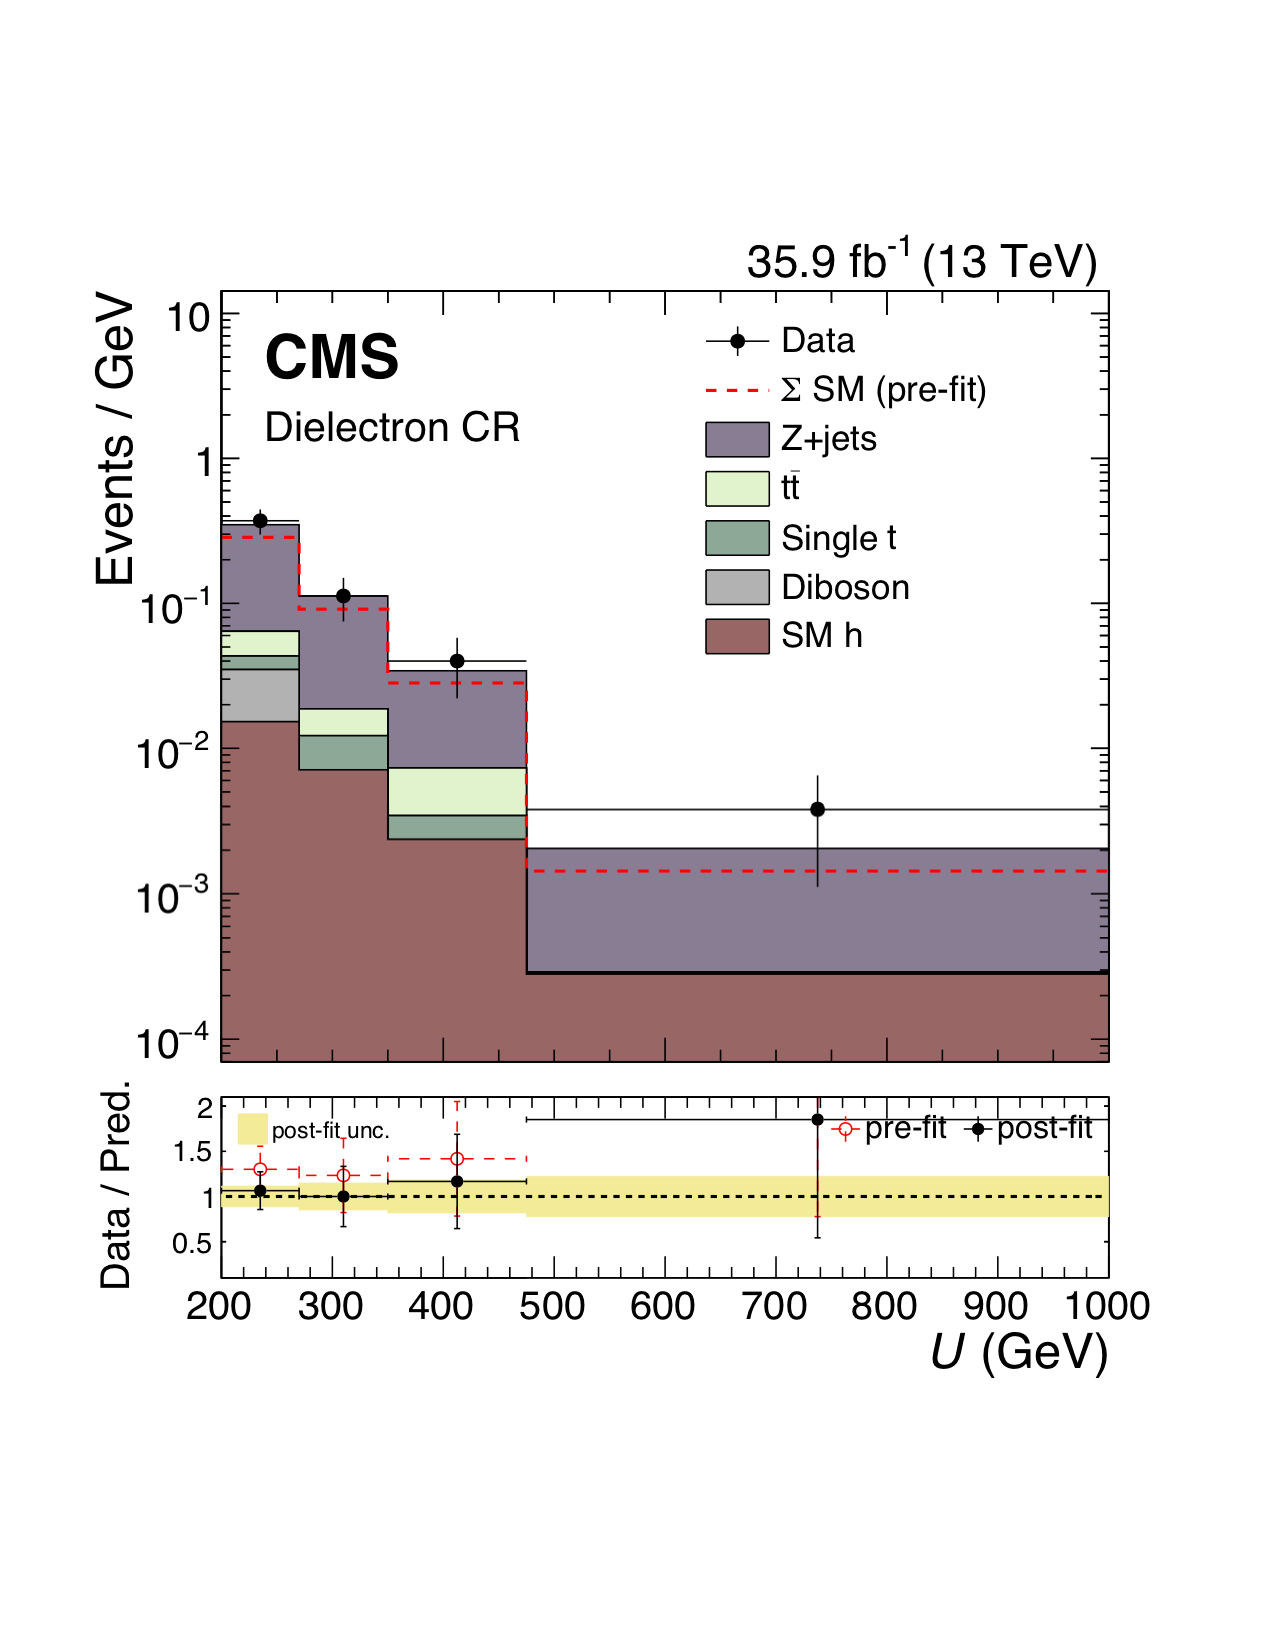
\includegraphics[width=0.36\textwidth]{figures/limits/MSDcorr_stackedPostfit_dielectron.pdf}}
 \subfloat{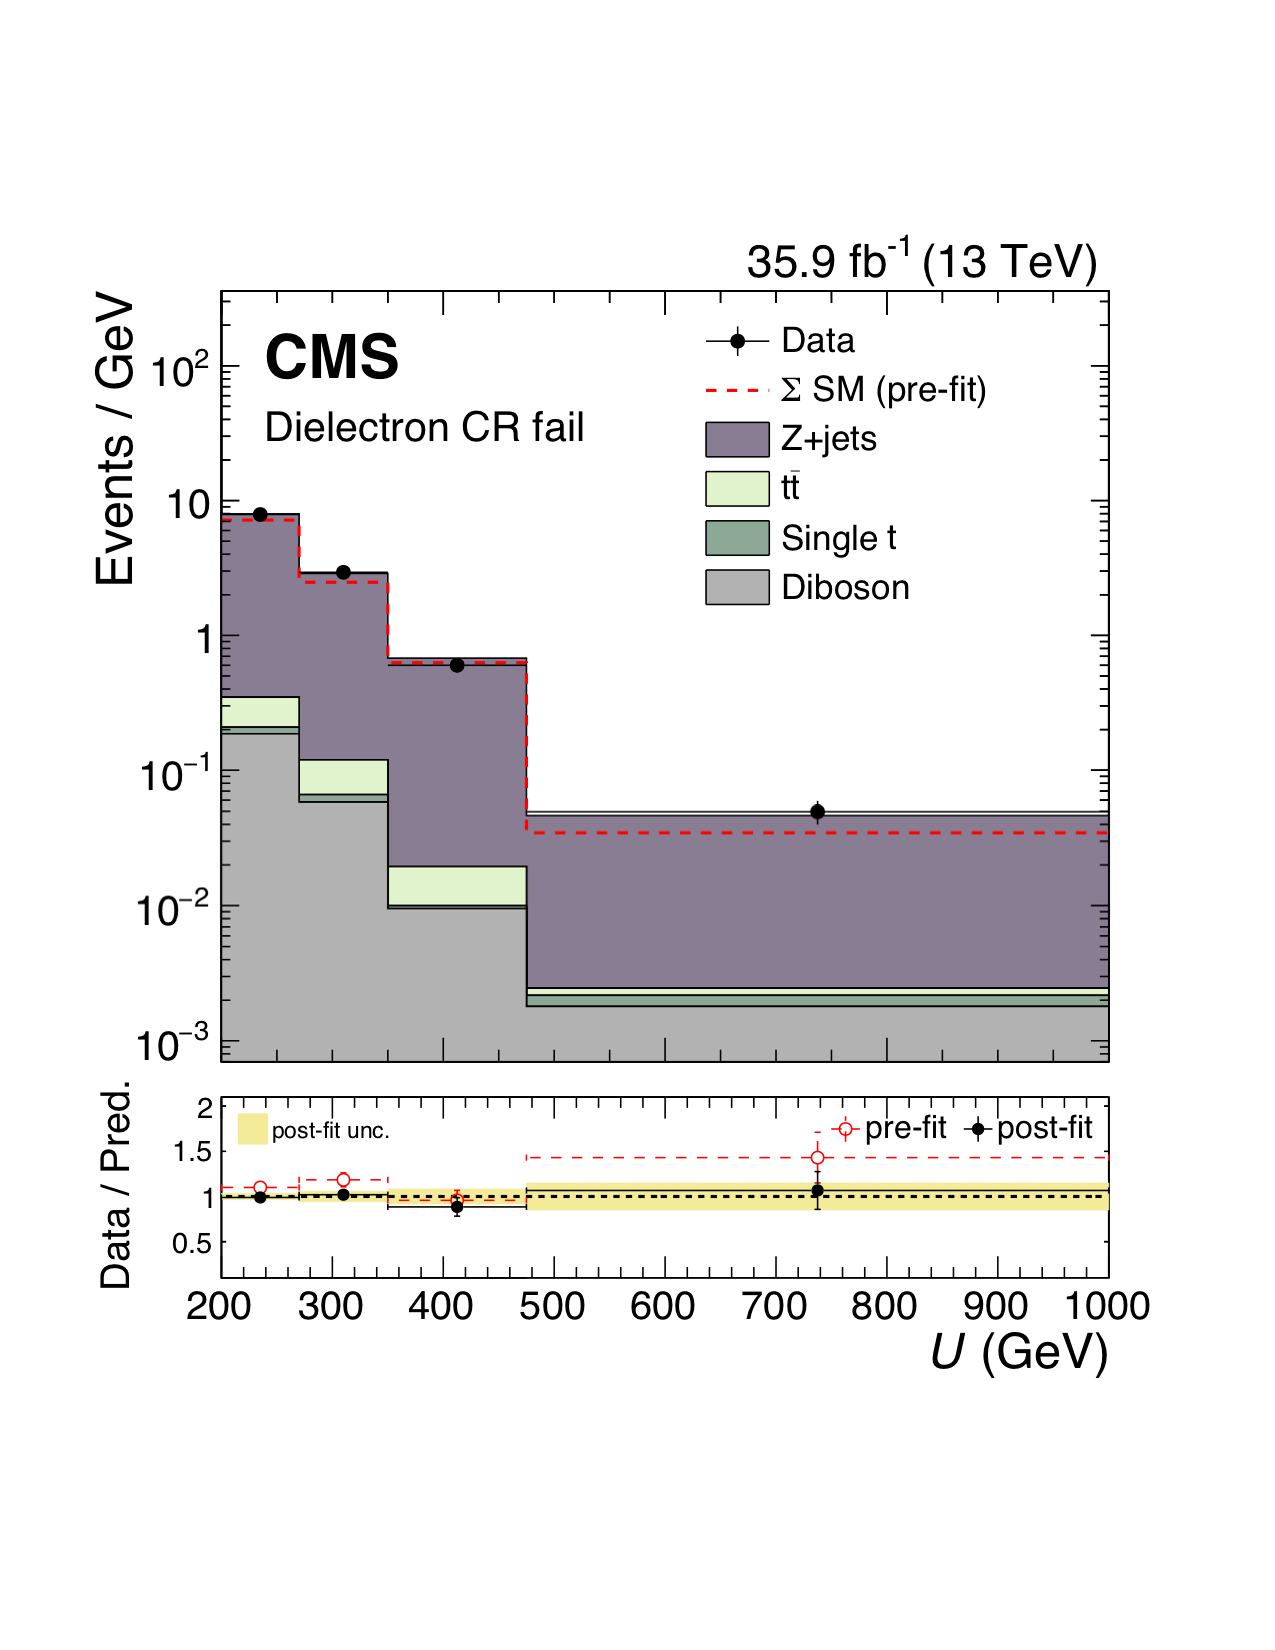
\includegraphics[width=0.36\textwidth]{figures/limits/MSDcorr_stackedPostfit_dielectron_fail.pdf}} \\
 \subfloat{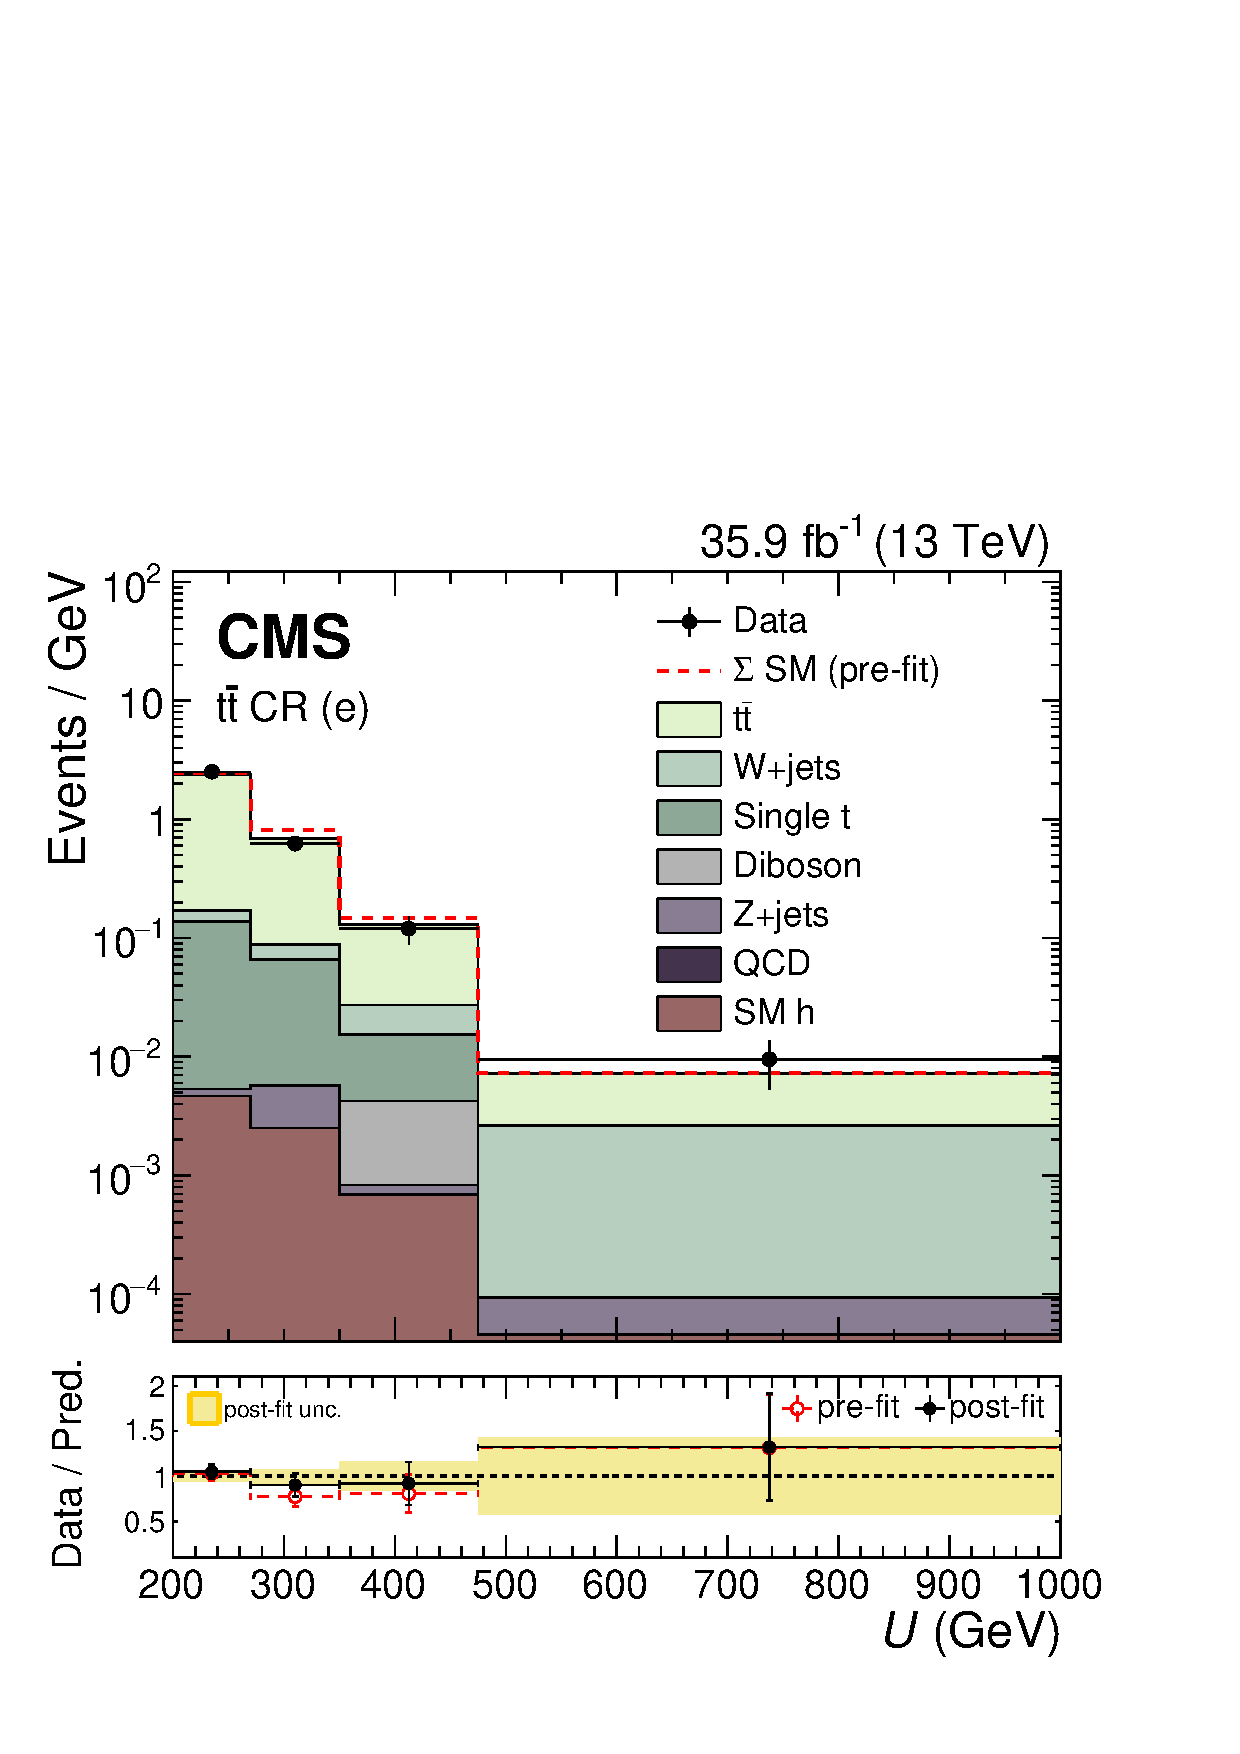
\includegraphics[width=0.36\textwidth]{figures/limits/MSDcorr_stackedPostfit_singleelectrontop.pdf}}
 \subfloat{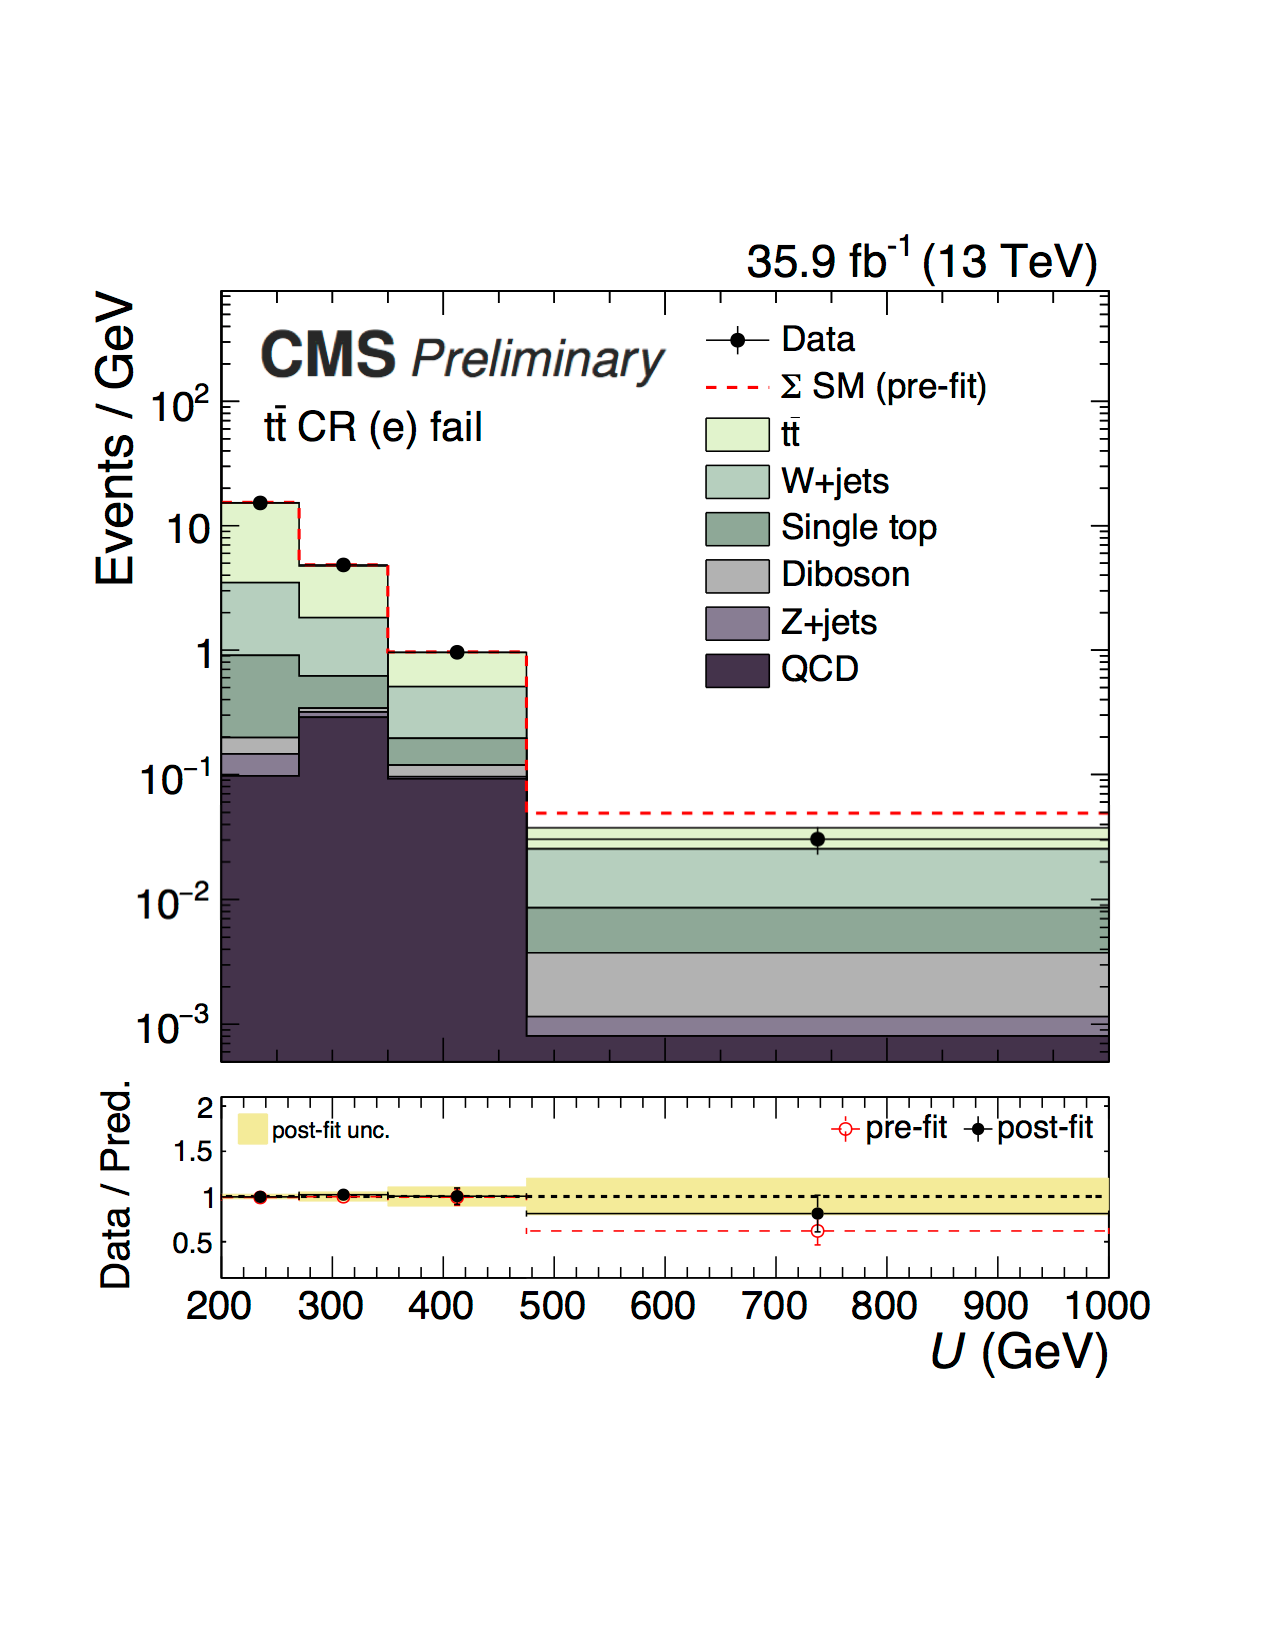
\includegraphics[width=0.36\textwidth]{figures/limits/MSDcorr_stackedPostfit_singleelectrontop_fail.pdf}} \\
 \subfloat{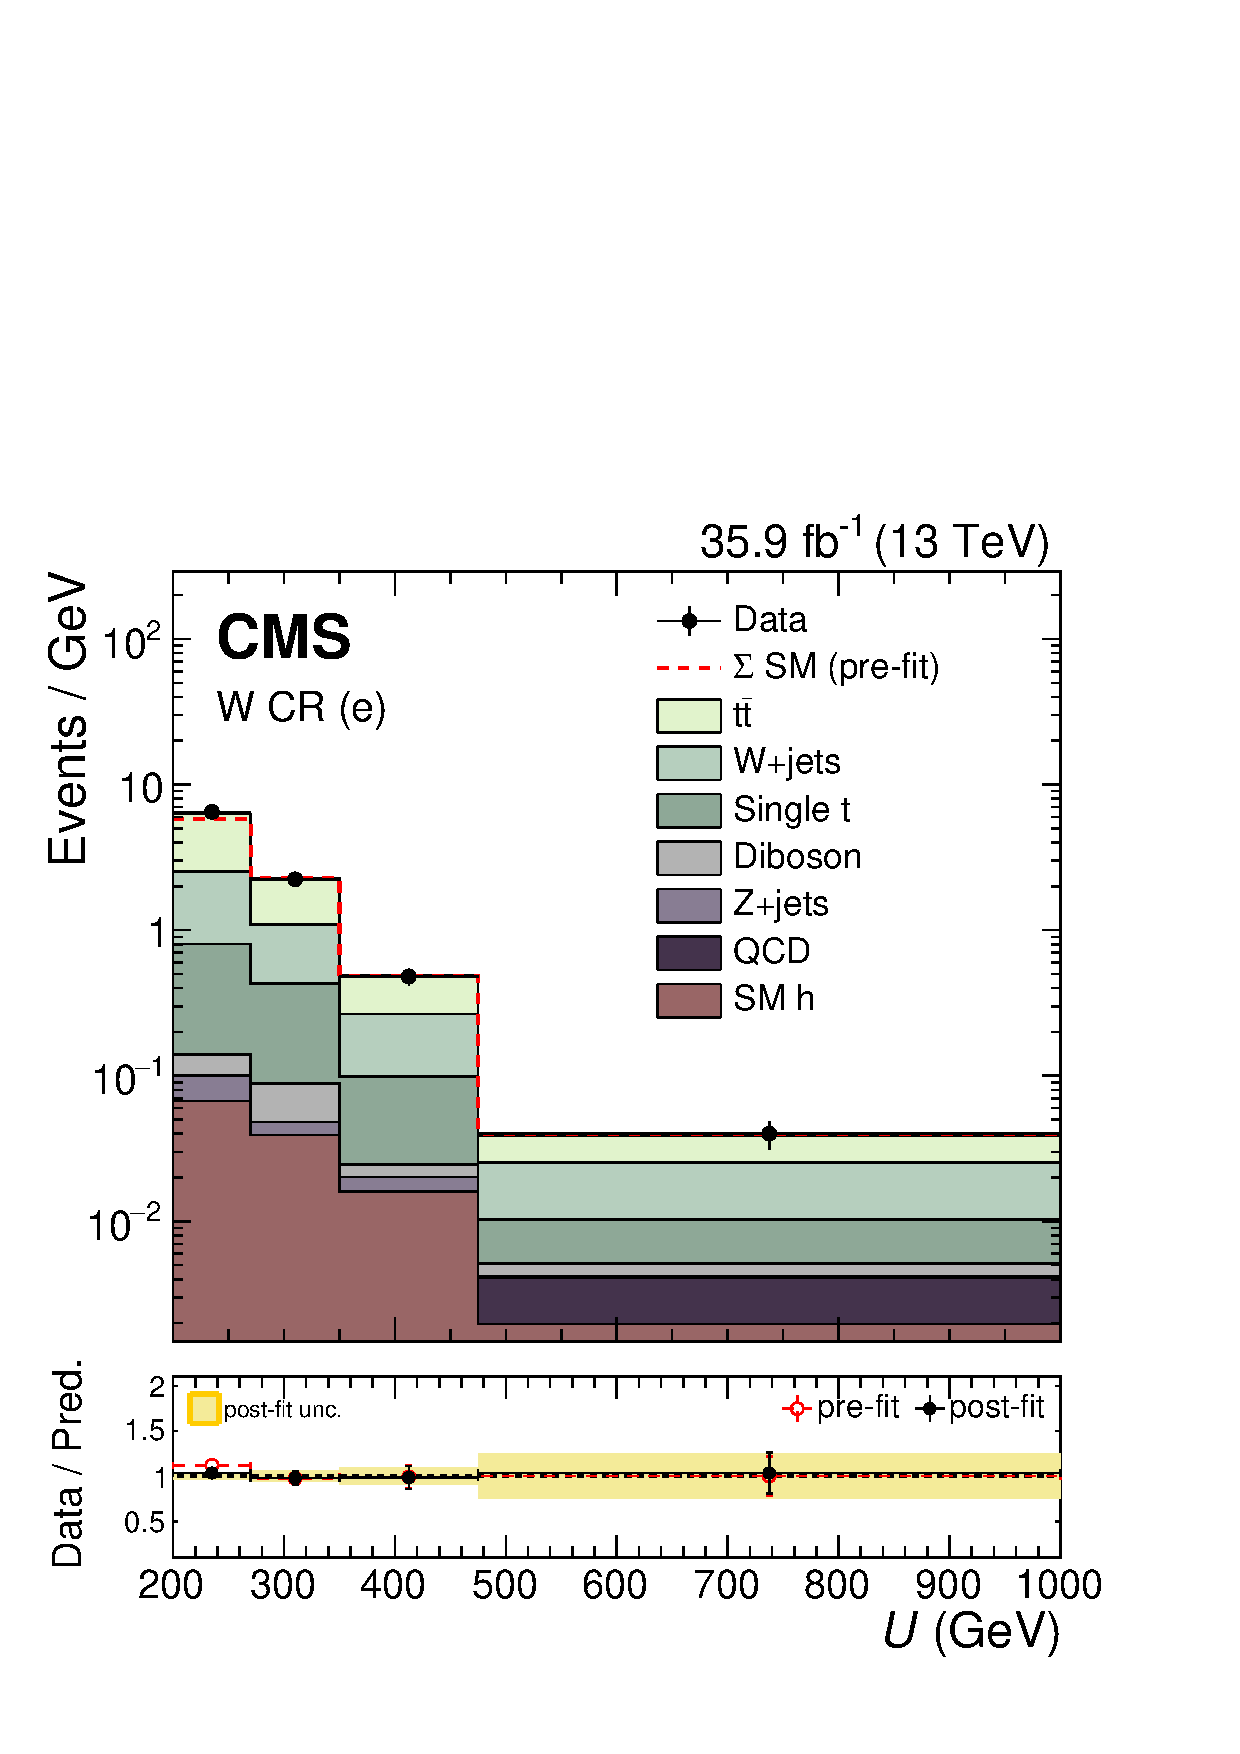
\includegraphics[width=0.36\textwidth]{figures/limits/MSDcorr_stackedPostfit_singleelectronw.pdf}}
 \subfloat{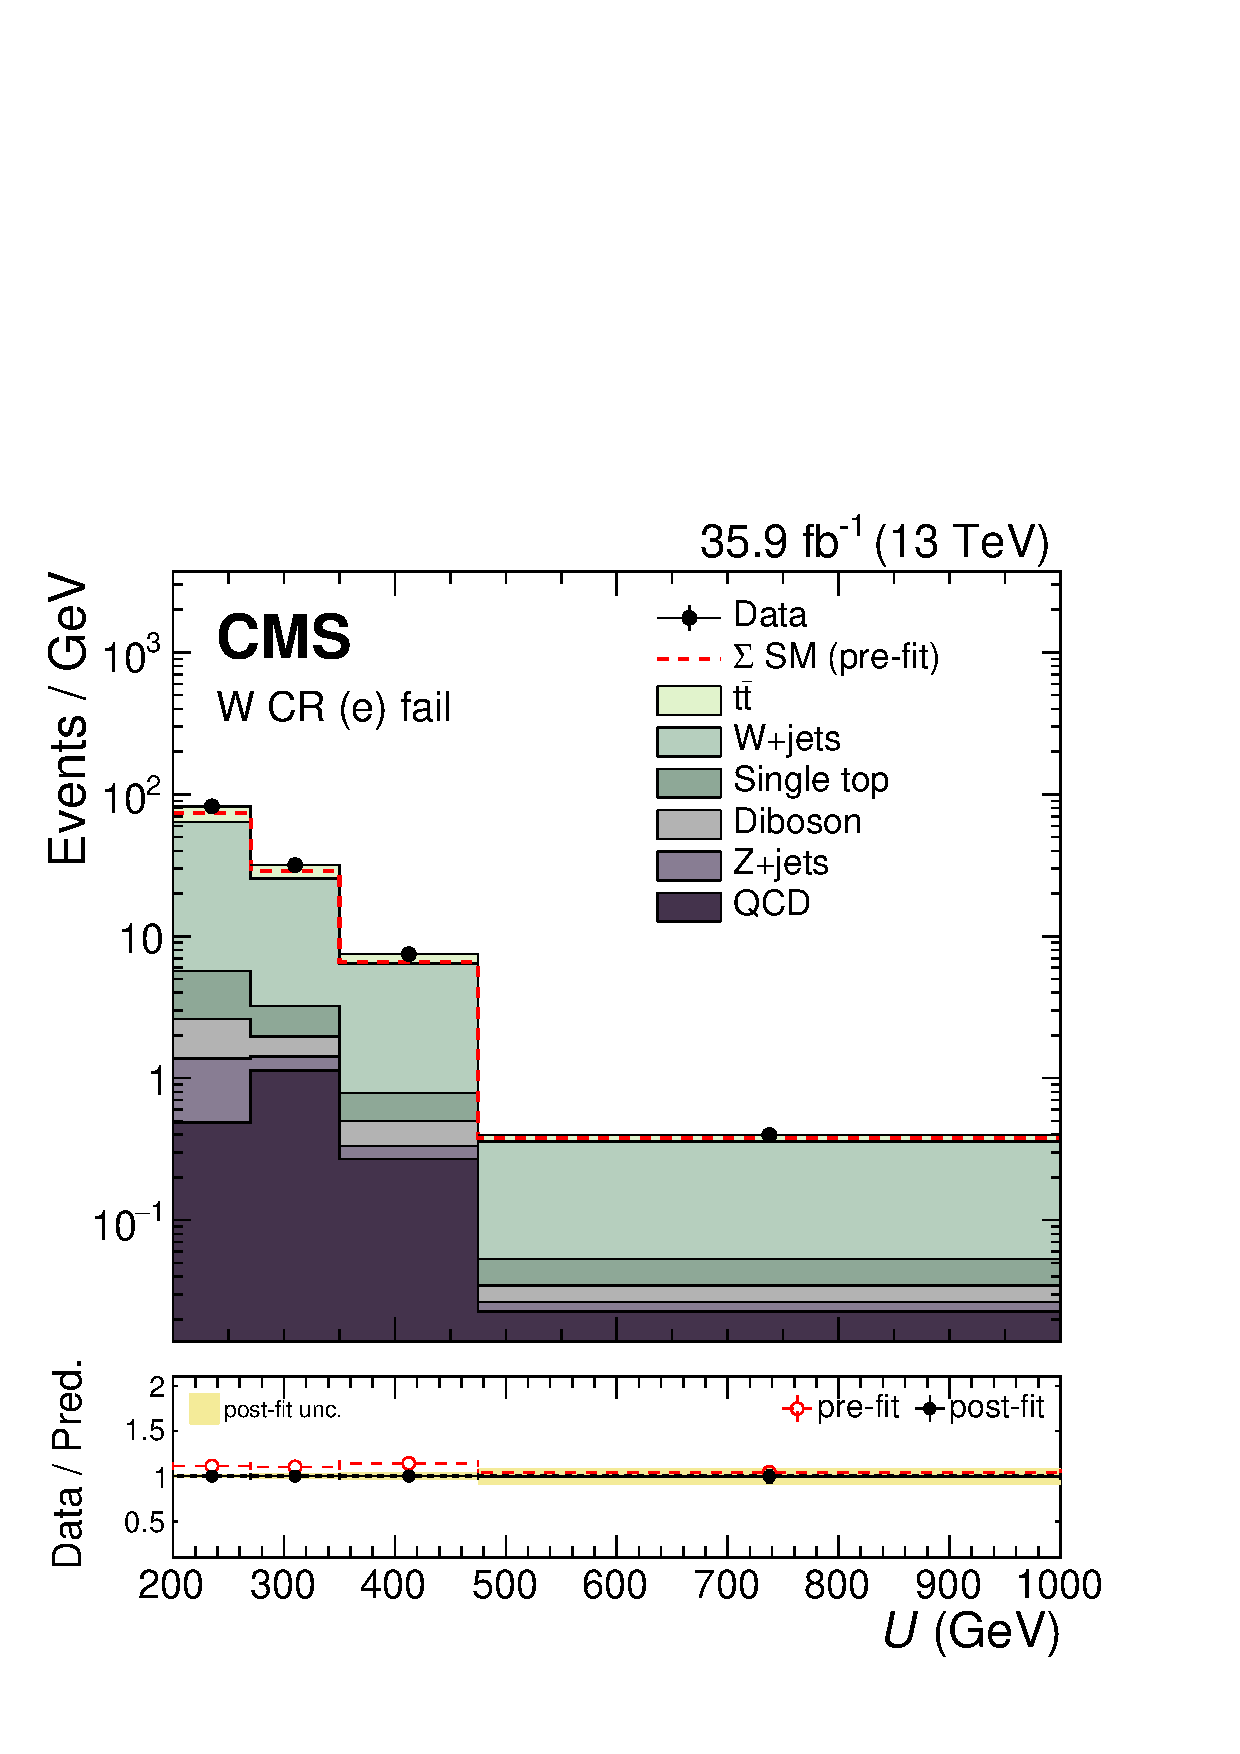
\includegraphics[width=0.36\textwidth]{figures/limits/MSDcorr_stackedPostfit_singleelectronw_fail.pdf}} \\
\caption{The $U$ distribution in the electron control regions before and after a background-only fit to data, including the data in the signal region in the likelihood. For the distributions on the left the CA15 jet passes the double-b tag requirement and for the distributions on the right it fails the double-b tag requirement.}
\label{Fig_cr_2}
\end{figure}


\begin{figure}
\centering
 \subfloat{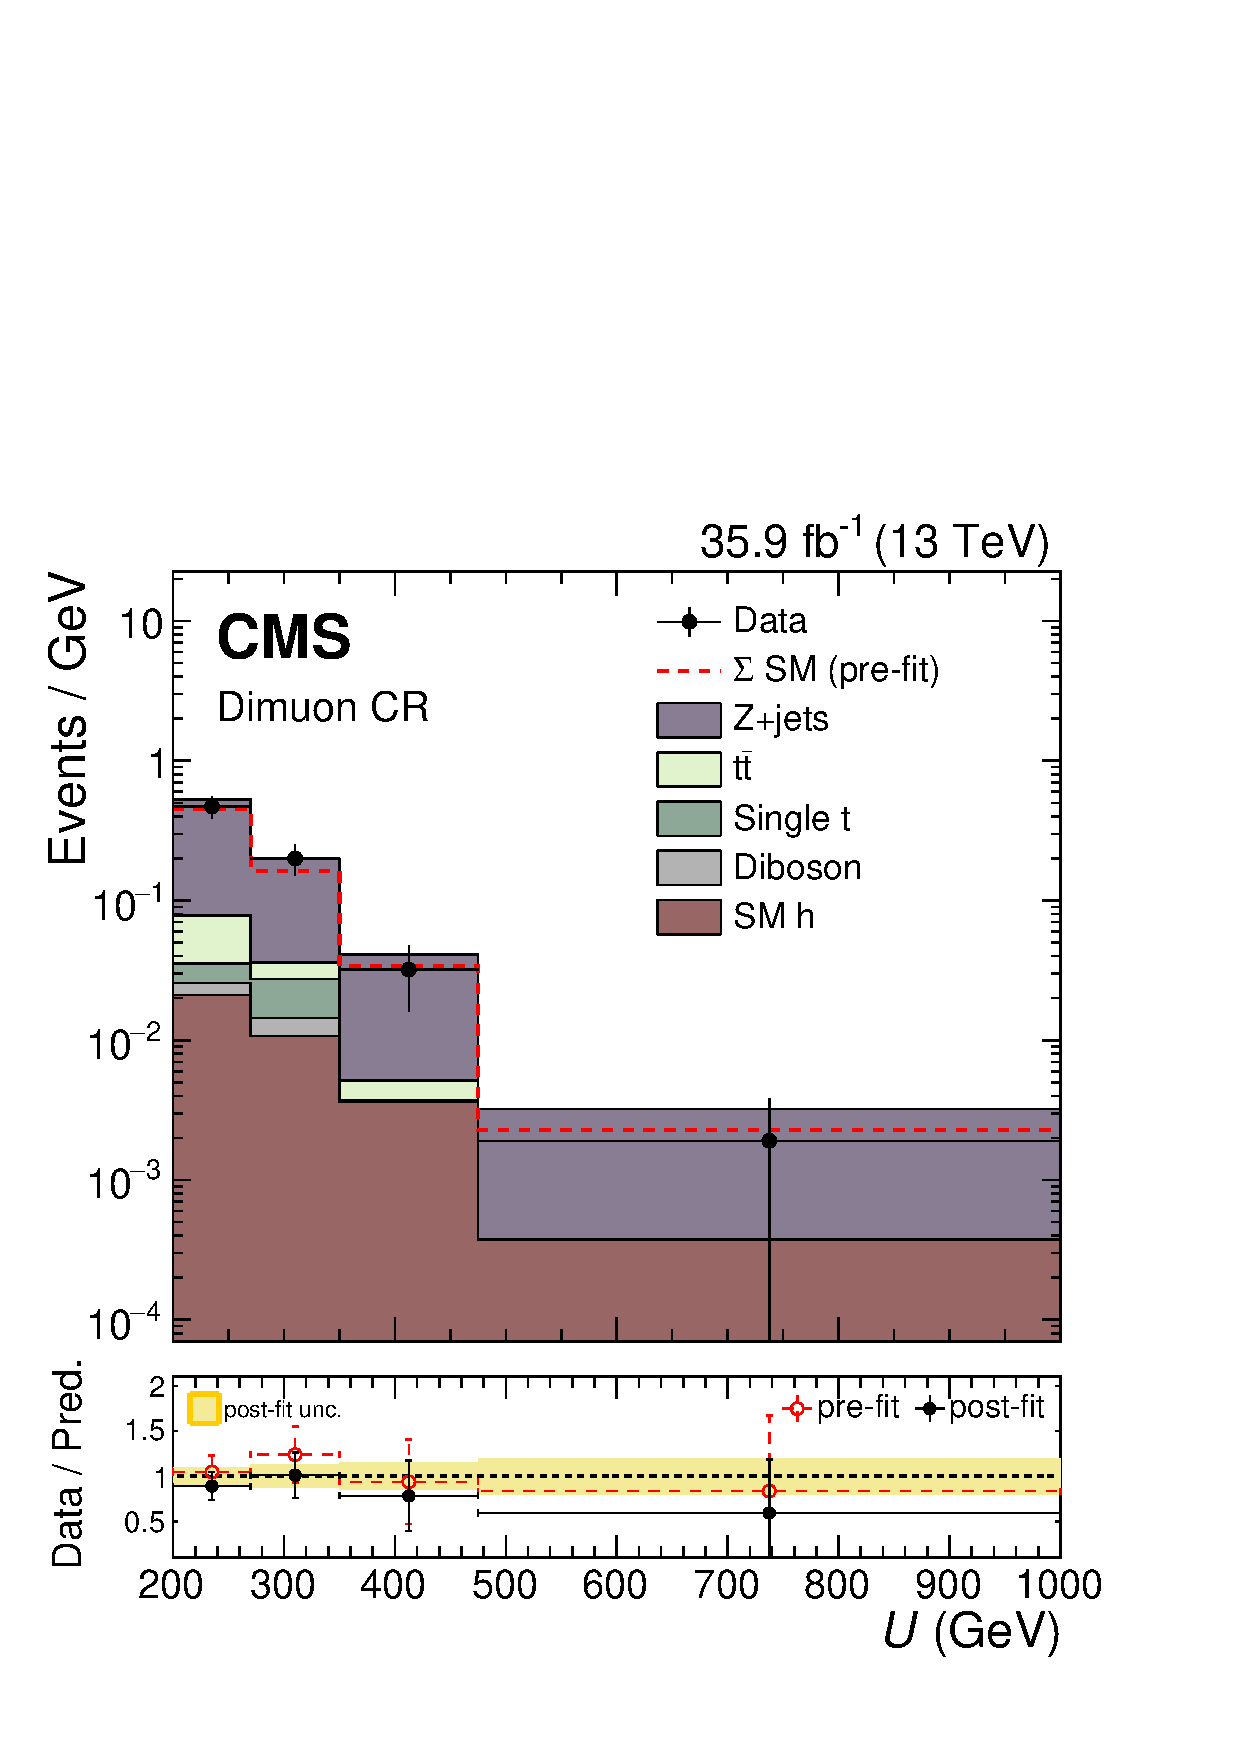
\includegraphics[width=0.36\textwidth]{figures/limits/MSDcorr_stackedPostfit_dimuon.pdf}}
 \subfloat{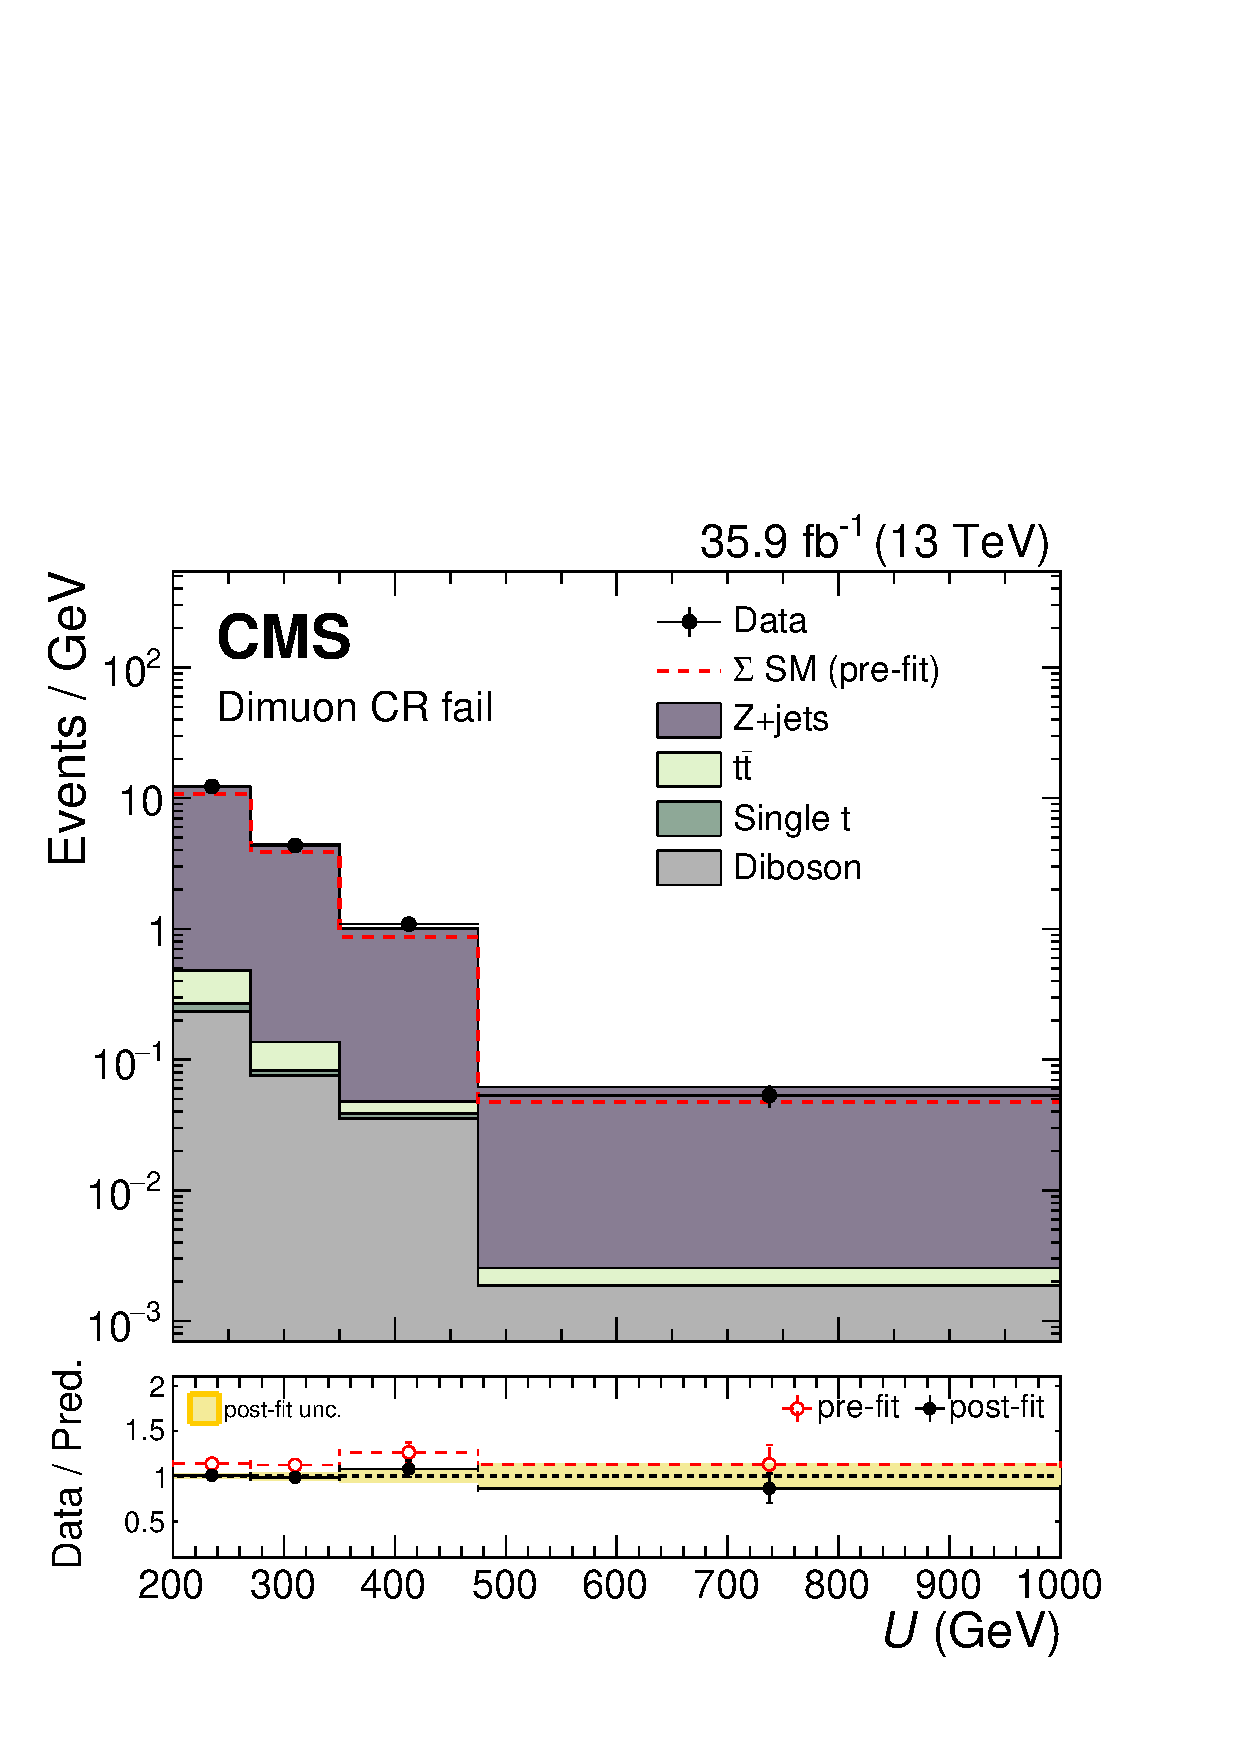
\includegraphics[width=0.36\textwidth]{figures/limits/MSDcorr_stackedPostfit_dimuon_fail.pdf}} \\
 \subfloat{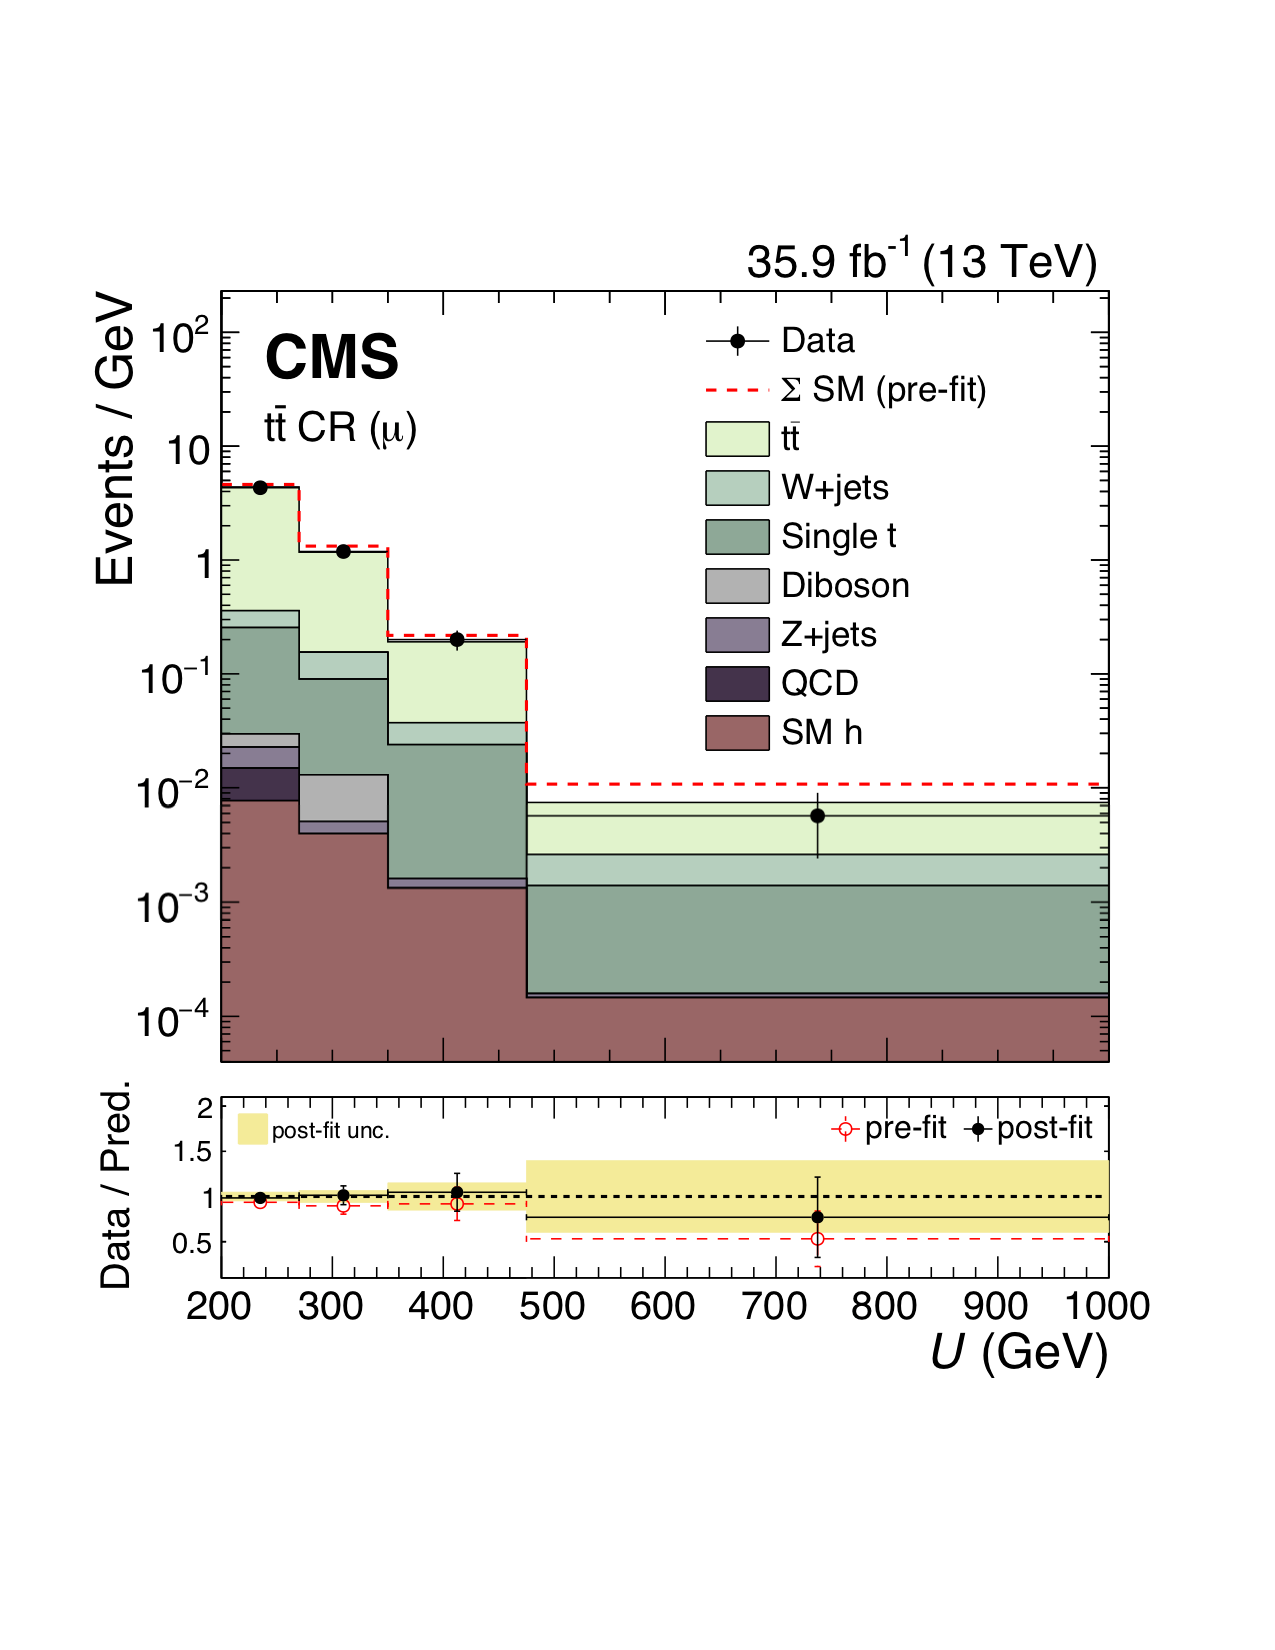
\includegraphics[width=0.36\textwidth]{figures/limits/MSDcorr_stackedPostfit_singlemuontop.pdf}}
 \subfloat{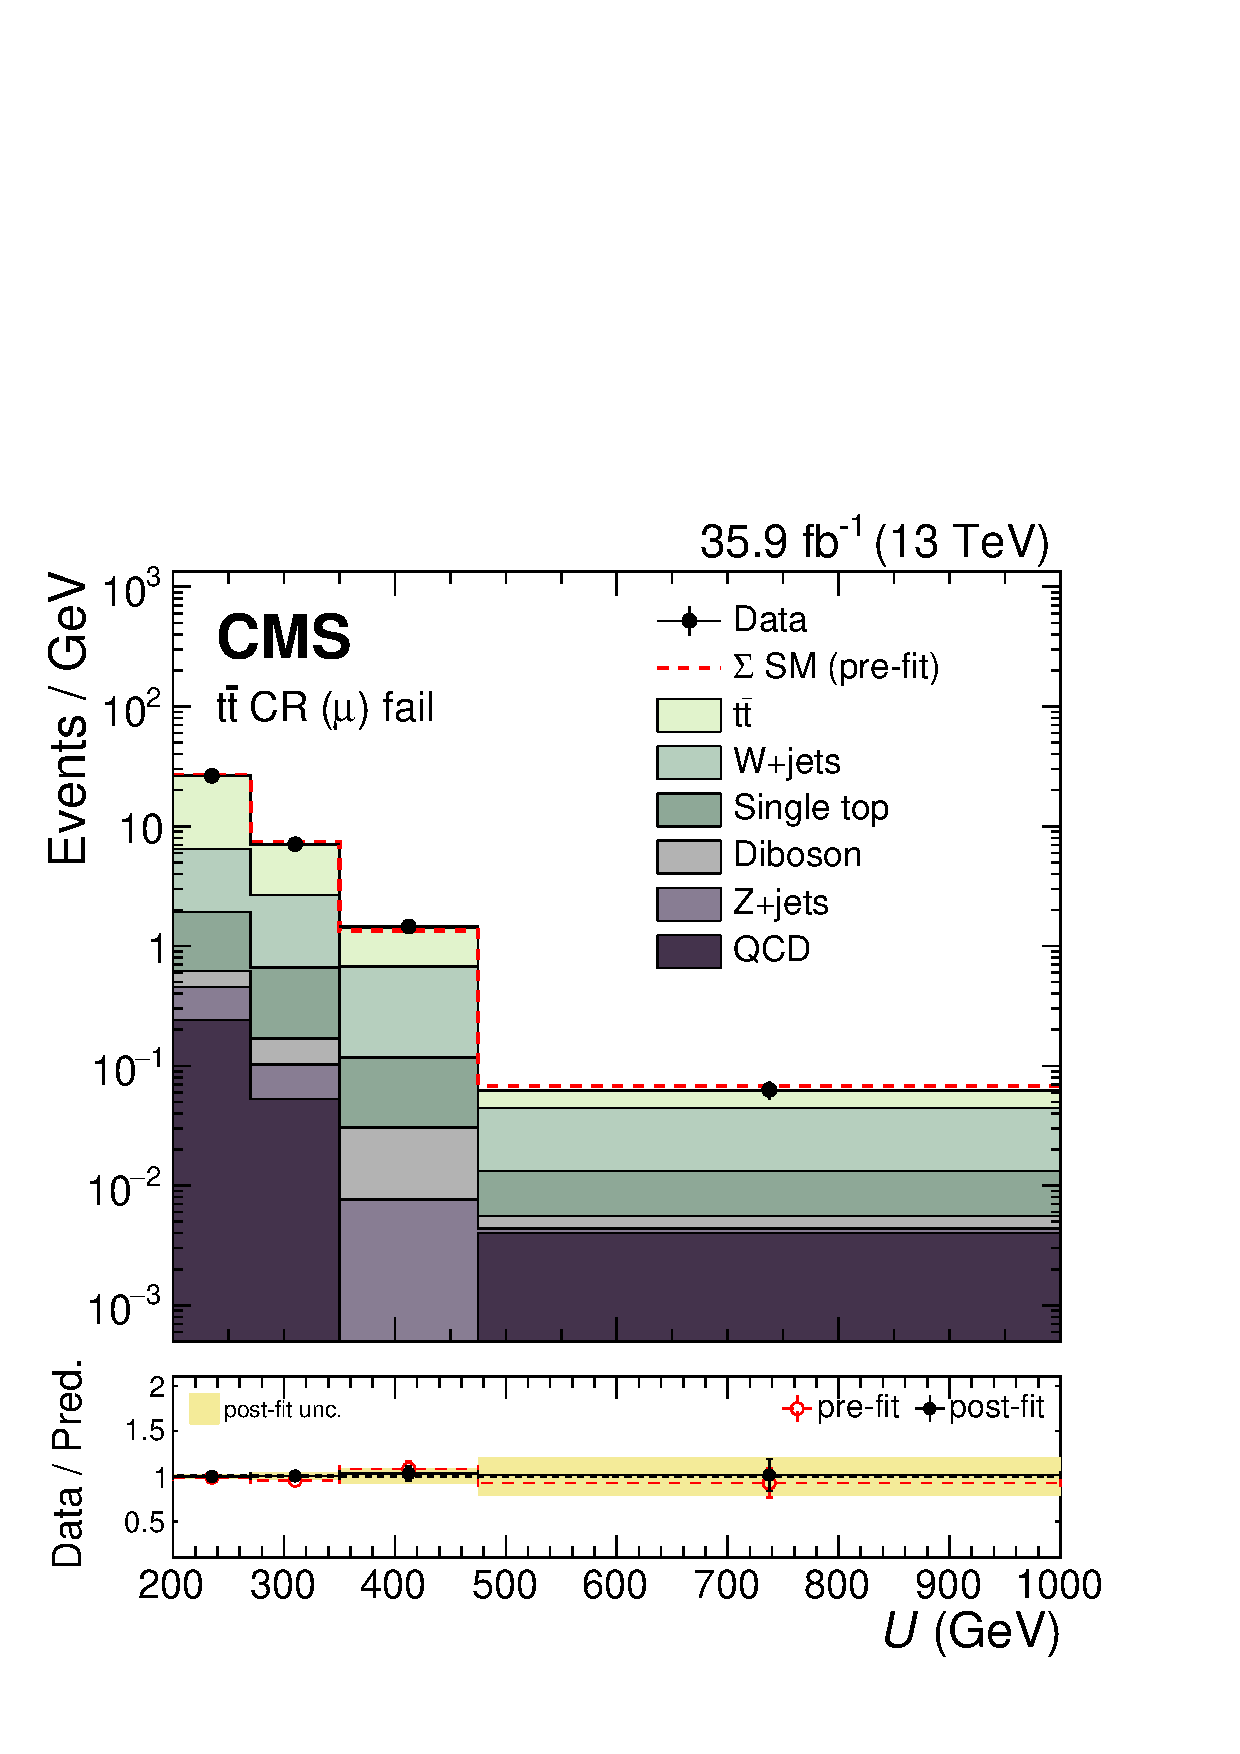
\includegraphics[width=0.36\textwidth]{figures/limits/MSDcorr_stackedPostfit_singlemuontop_fail.pdf}} \\
 \subfloat{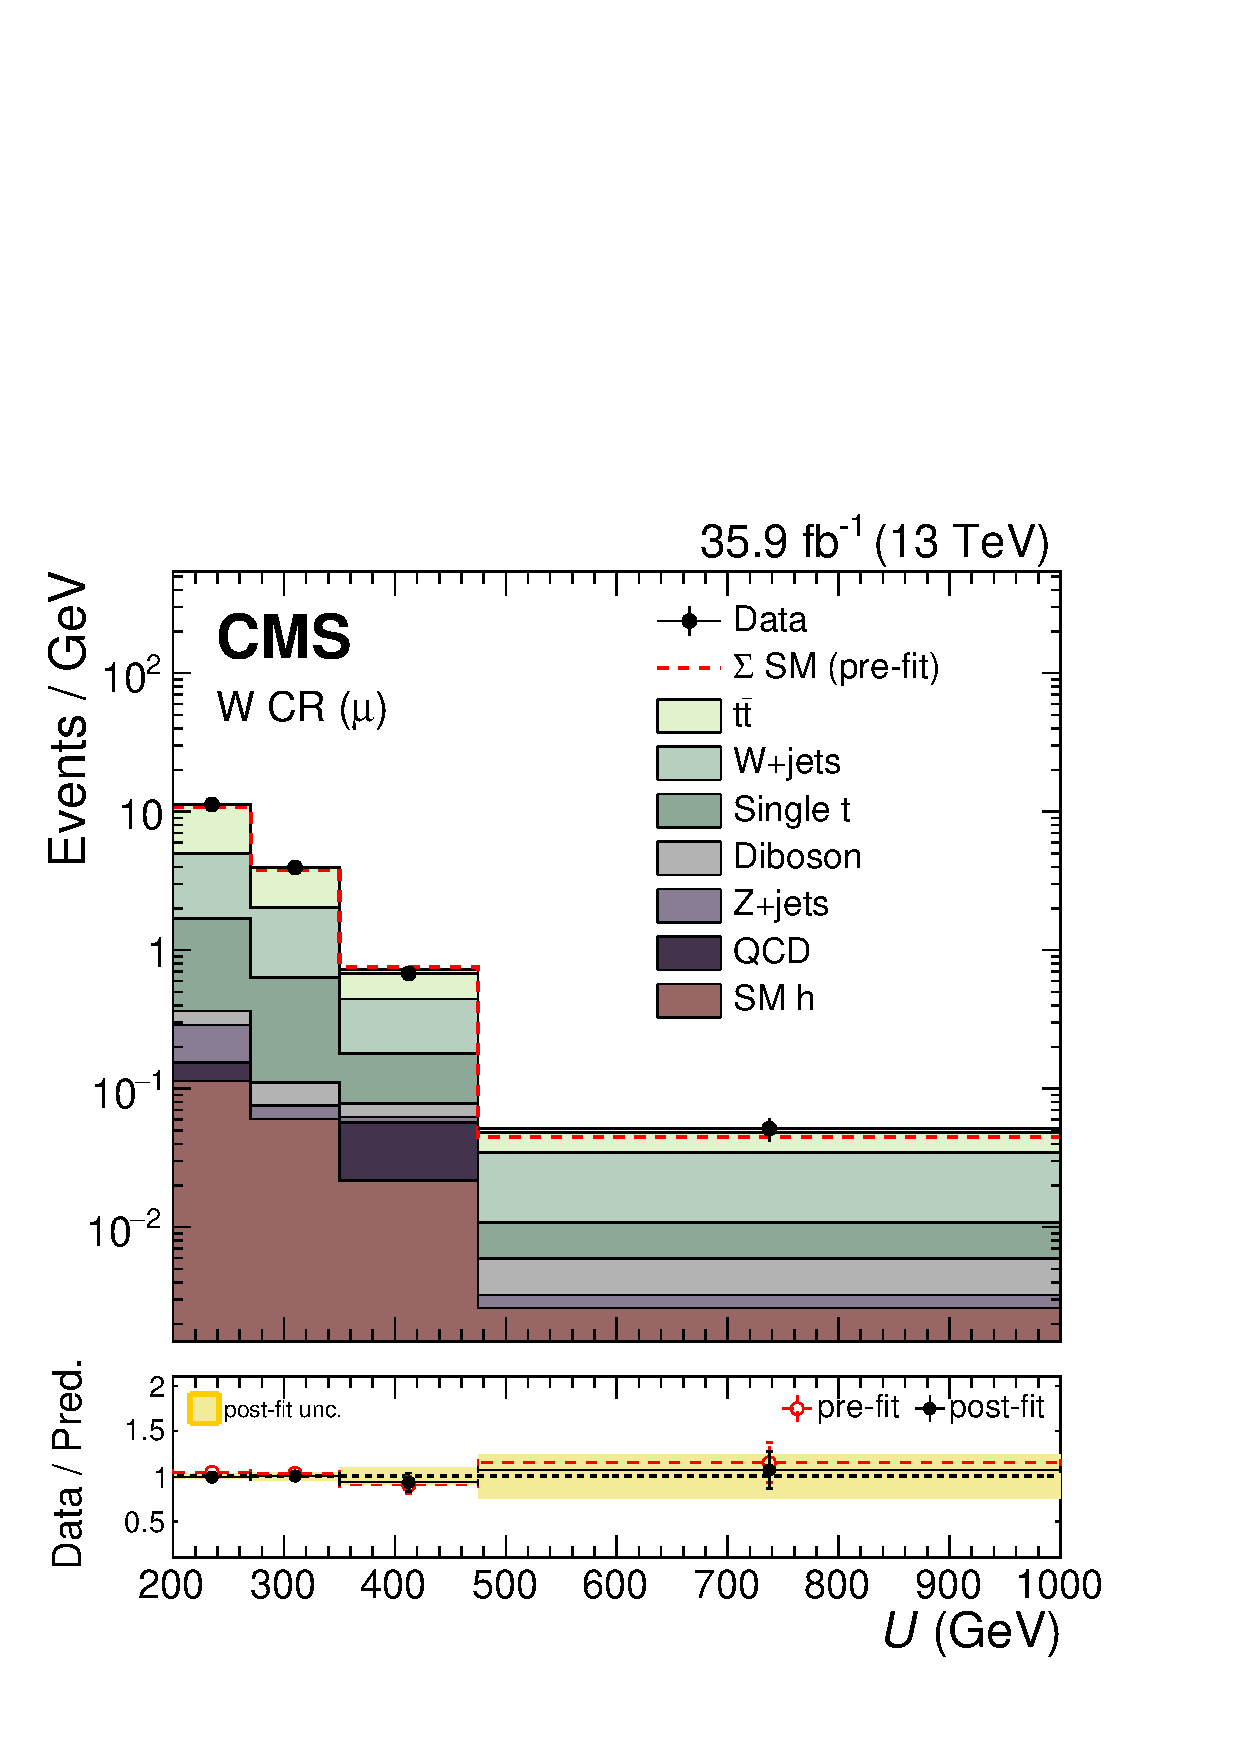
\includegraphics[width=0.36\textwidth]{figures/limits/MSDcorr_stackedPostfit_singlemuonw.pdf}}
 \subfloat{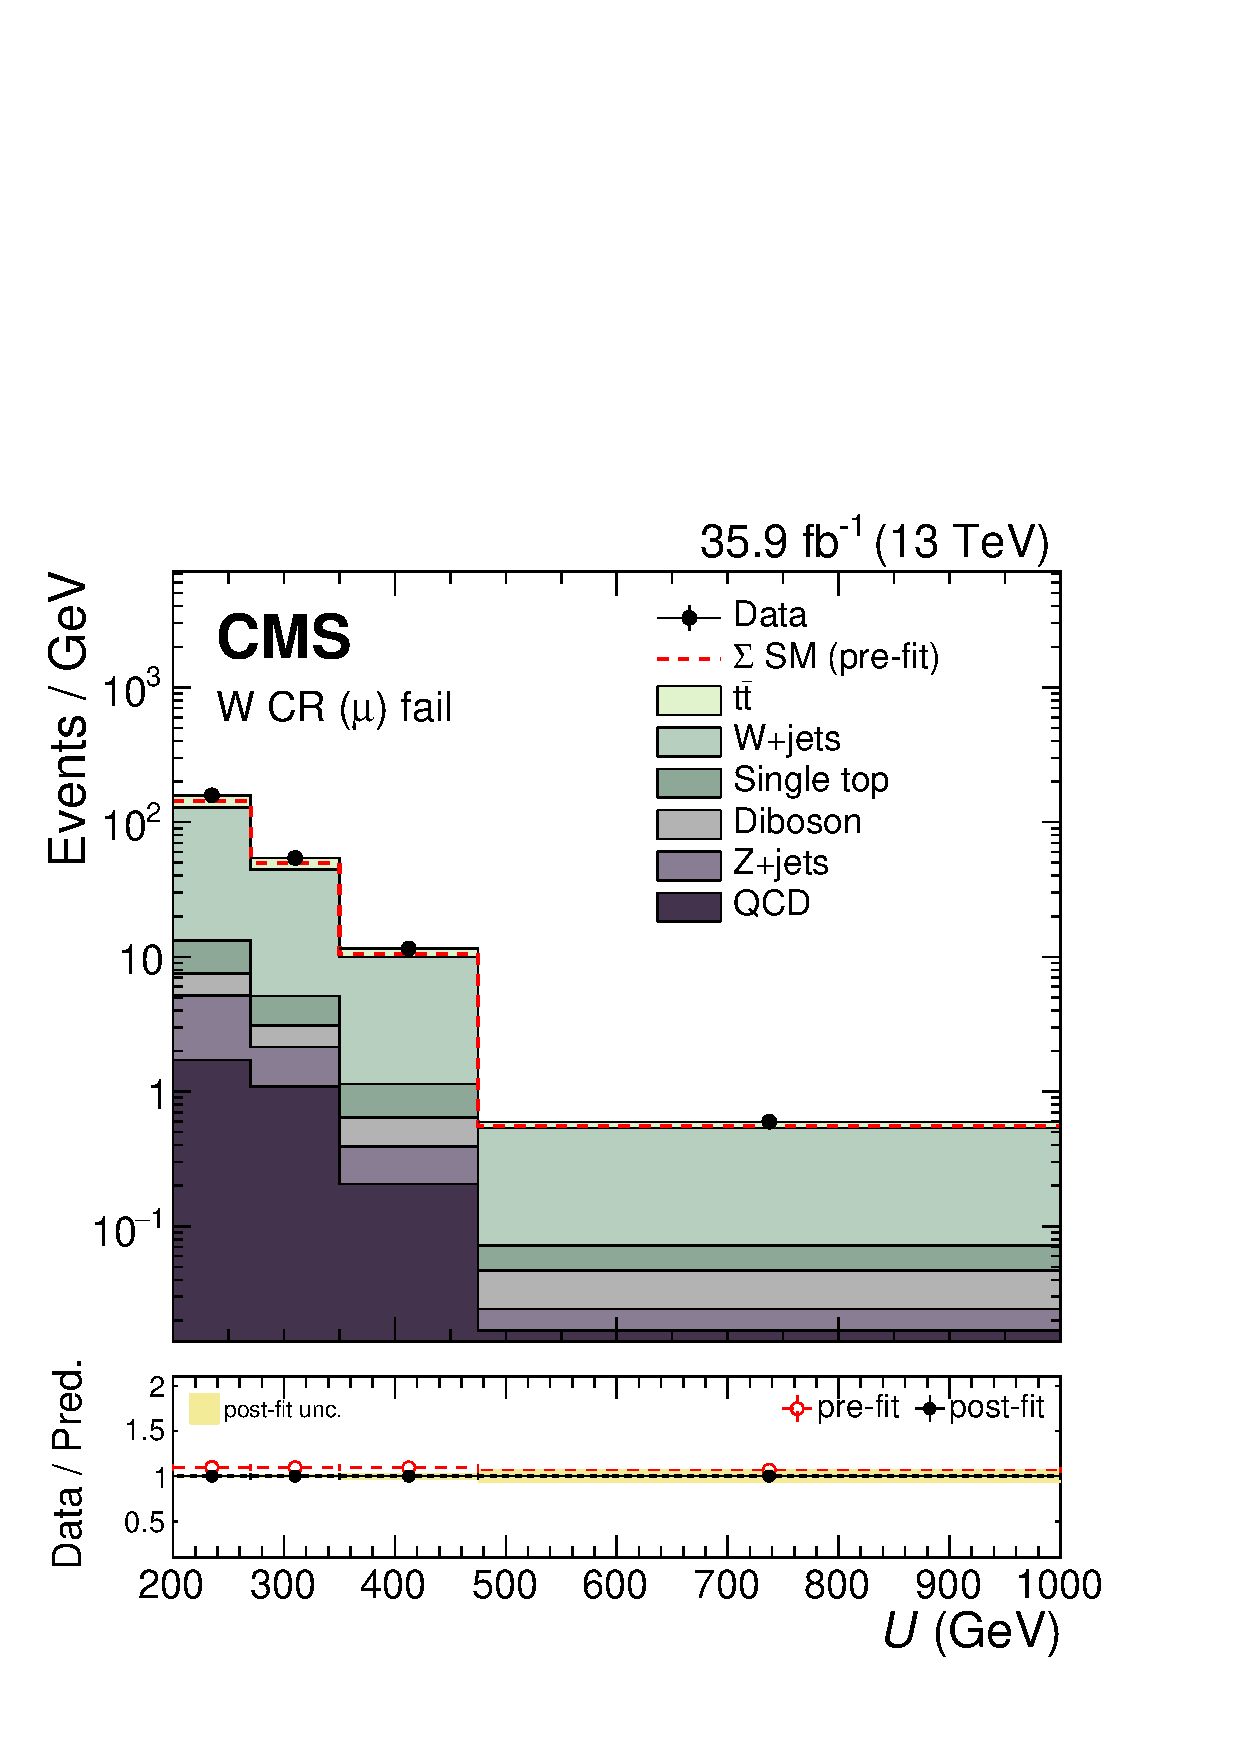
\includegraphics[width=0.36\textwidth]{figures/limits/MSDcorr_stackedPostfit_singlemuonw_fail.pdf}} \\
 \caption{The $U$ distribution in the muon control regions before and after a background-only fit to data, including the data in the signal region in the likelihood. For the distributions on the left the CA15 jet passes the double-b tag requirement and for the distributions on the right it fails the double-b tag requirement.}
\label{Fig_cr_1}
\end{figure}

No significant excess over the SM background expectation is observed in the SR. The results of this search are interpreted in terms of upper limits on the signal strength modifier $\mu=\sigma/\sigma_\text{theory}$, where $\sigma_\text{theory}$ is the predicted production cross 
section of DM candidates in association with a Higgs boson and $\sigma$ is the upper limit on the observed cross section. 
The upper limits are calculated at 95\% confidence level (CL) using a modified frequentist method (CL$_s$) \cite{yellowReport, bib:CLS1, bib:CLS2} computed with an asymptotic approximation \cite{bib:CLS3}. 


%\begin{table}\footnotesize
%\begin{center}
%  \caption{Per-\ptmiss-bin post-fit event yield expectations for the SM backgrounds in the signal region when masking the signal region data from the likelihood fit. Uncertainties quoted on the predictions include systematic and statistical uncertainties.}
%\begin{tabular}{l r r r r}
%  \hline\hline
%\ptmiss-bin         & 200-270\,GeV          & 270-350\,GeV          & 350-475\,GeV          & $>475$\,GeV         \\
%\hline
%Z+jets          &$ 239.2\pm37.9 $       & $93.3\pm14.4$         & $31.1\pm5.5$          & $10.0\pm2.2$       \\
%\ttbar          &$ 200.0\pm13.3 $       & $52.3\pm5.1$          & $11.1\pm2.0$          & $0.7\pm0.4$        \\
%W+jets          &$ 119.8\pm22.4 $       & $44.3\pm8.9$          & $8.3\pm1.9$           & $2.8\pm0.9$            \\
%Single top      &$21.0\pm4.3 $          & $6.1\pm1.3$           & $0.9\pm0.2$           & $0.2\pm0.1$         \\
%Diboson         &$ 16.0\pm3.1  $        & $7.6\pm1.5$           & $2.4\pm0.5$           & $1.0\pm0.2$ \\
%SM h             &$ 12.6\pm1.4 $      & $ 6.6\pm0.7$           & $ 3.3 \pm 0.3$        & $ 1.3\pm 0.1$      \\
%\hline
%$\Sigma~(\text{SM})$ & $608.3\pm41.8$ & $210.2 \pm 15.9$       & $57.1\pm5.7$          & $16.0 \pm 2.2$ \\
%\hline
%Data            & $619$       & $ 214$        & $59$          & $ 21$ \\
%\hline\hline
%  \end{tabular}
%\label{tab:eventYieldTable_masked}
%\end{center}
%\end{table}


Figure~\ref{fig:limits_2hdma} shows the upper limits on $\mu$ for the three scans ($m_A$, $\sin\theta$, and $\tan\beta$) performed.
For the 2HDM+$a$ model, $m_\text{A}$ masses are excluded between 500 and 900\GeV for $m_\text{a}=150\GeV$, $\sin\theta=0.35$ and $\tan\beta=1$. Mixing angles with $0.35<\sin\theta<0.75$ are excluded for $m_\text{A}=600\GeV$ and $m_\text{a}=200\GeV$, assuming $\tan\beta=1$. Also excluded are $\tan\beta$ values between 0.5 and 2.0 (1.6) for $m_\text{a}=100$ (150)\GeV and $m_\text{A}=600\GeV$, given $\sin\theta=0.35$. These are the first experimental limits on the 2HDM+$a$ model.

\begin{figure}[htbp]
  \centering
  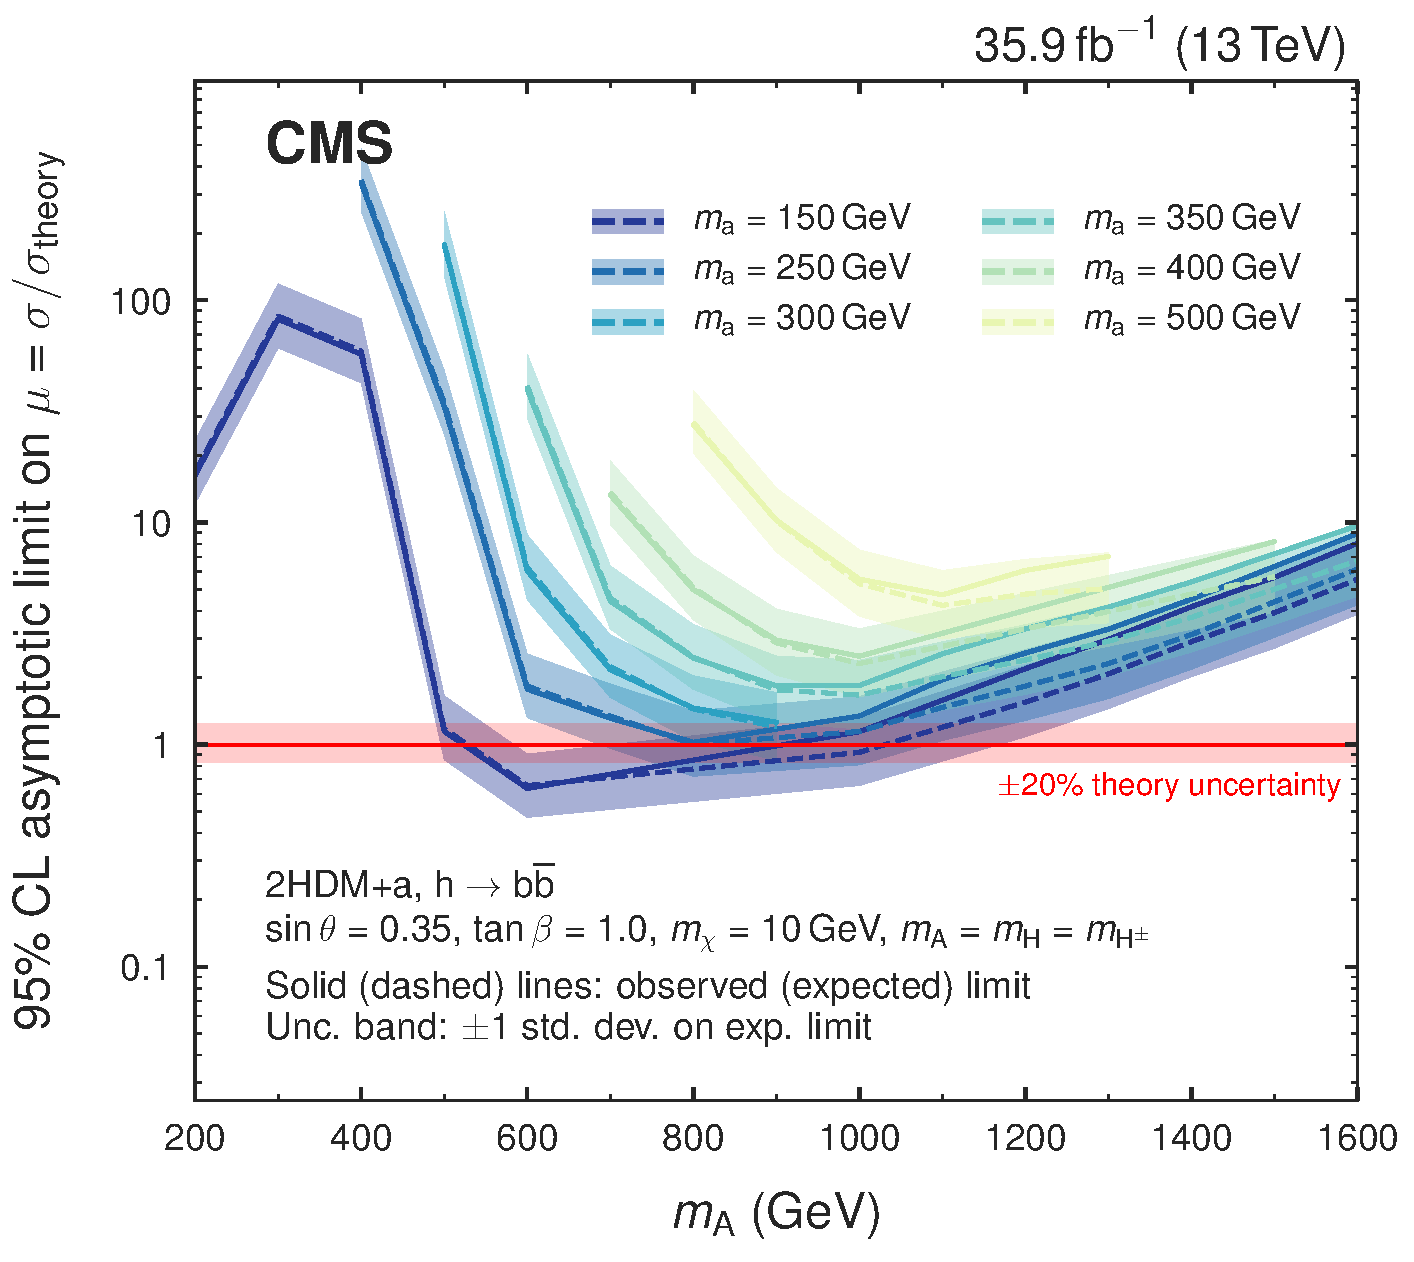
\includegraphics[width=0.475\textwidth]{figures/limits/limits_2hdma_mass.pdf}
  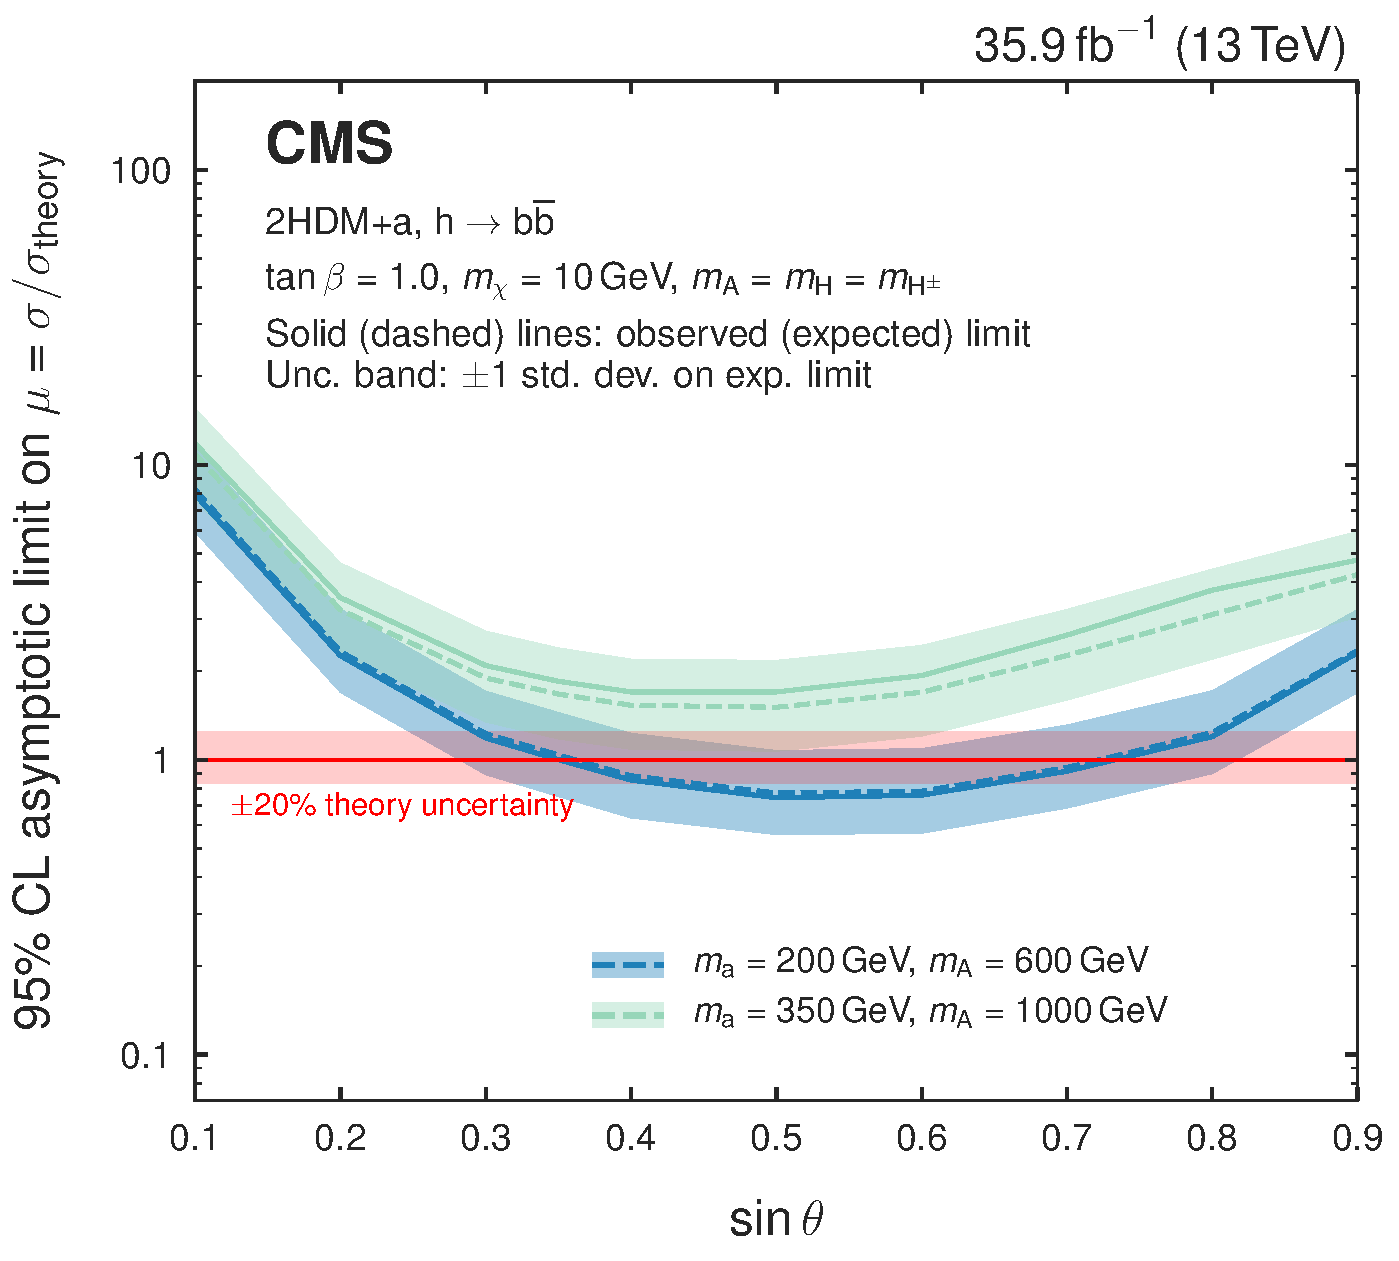
\includegraphics[width=0.475\textwidth]{figures/limits/limits_2hdma_sinp.pdf}\\
  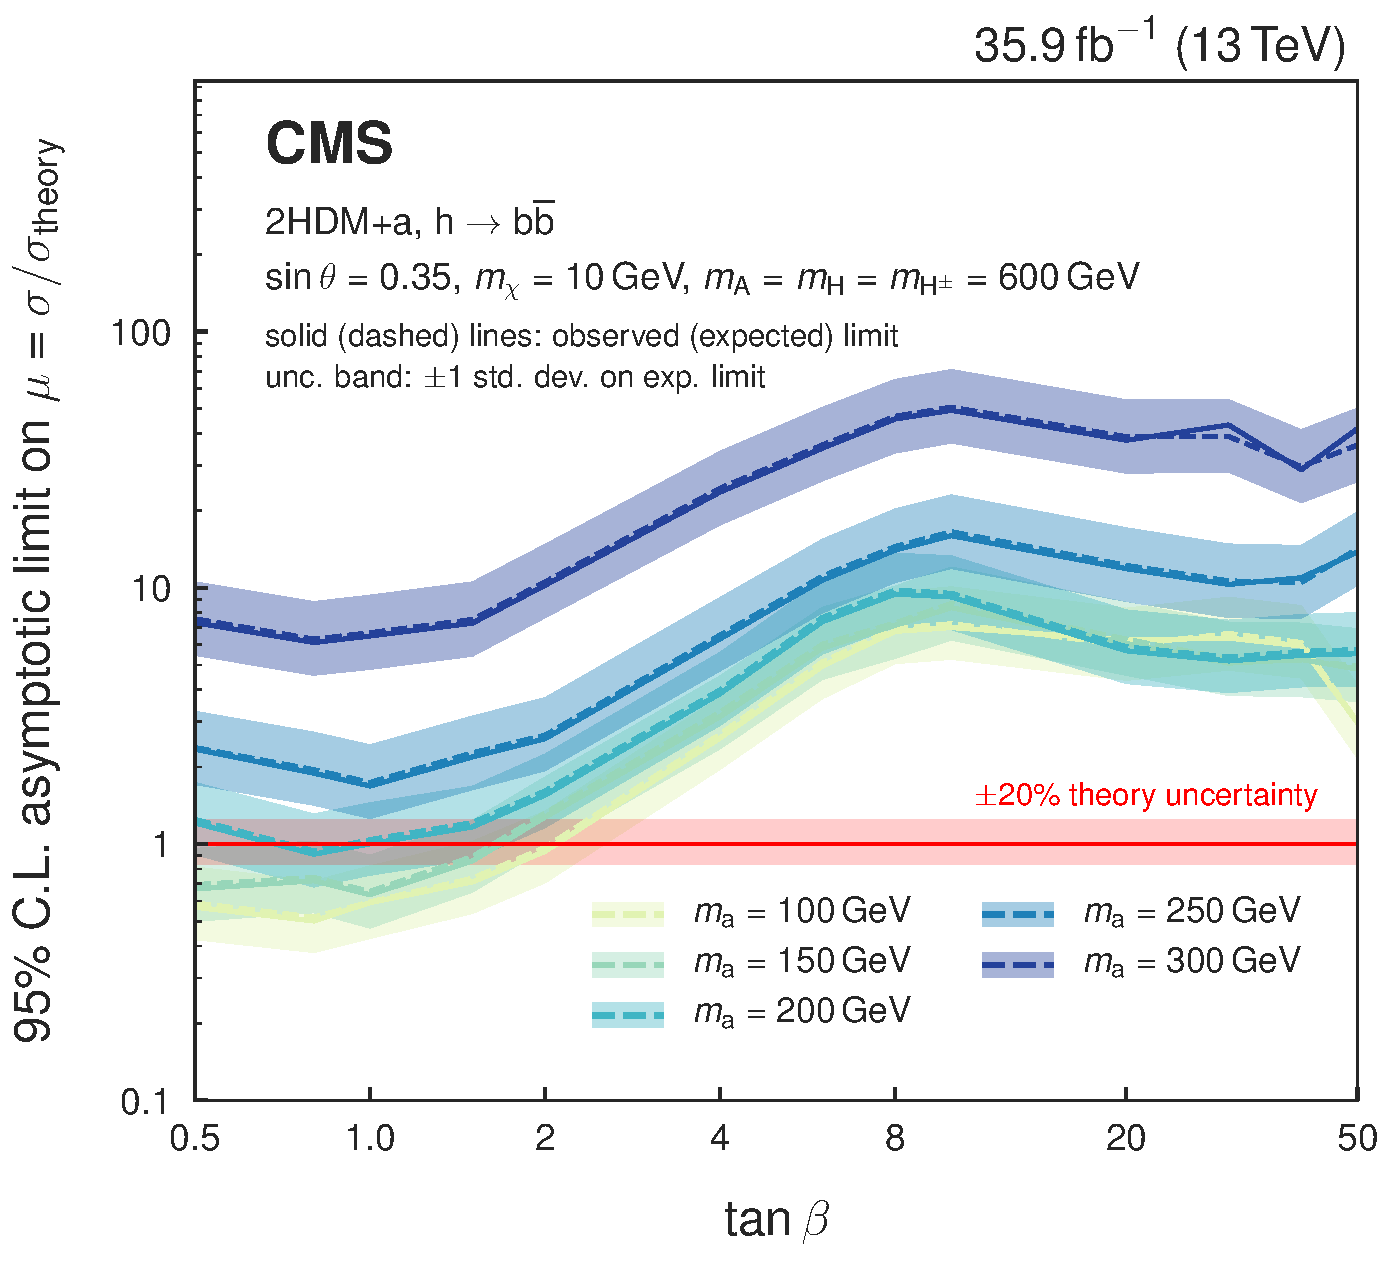
\includegraphics[width=0.475\textwidth]{figures/limits/limits_2hdma_tanb.pdf}\\
  \caption{Upper limits on the signal strength modifier for the 2HDM+$a$ model when scanning $m_\text{A}$ and $m_\text{a}$ (upper left), the mixing angle $\theta$ (upper right), or $\tan\beta$ (lower).}
  \label{fig:limits_2hdma}
\end{figure}


\begin{figure}[htbp]
  \centering
%  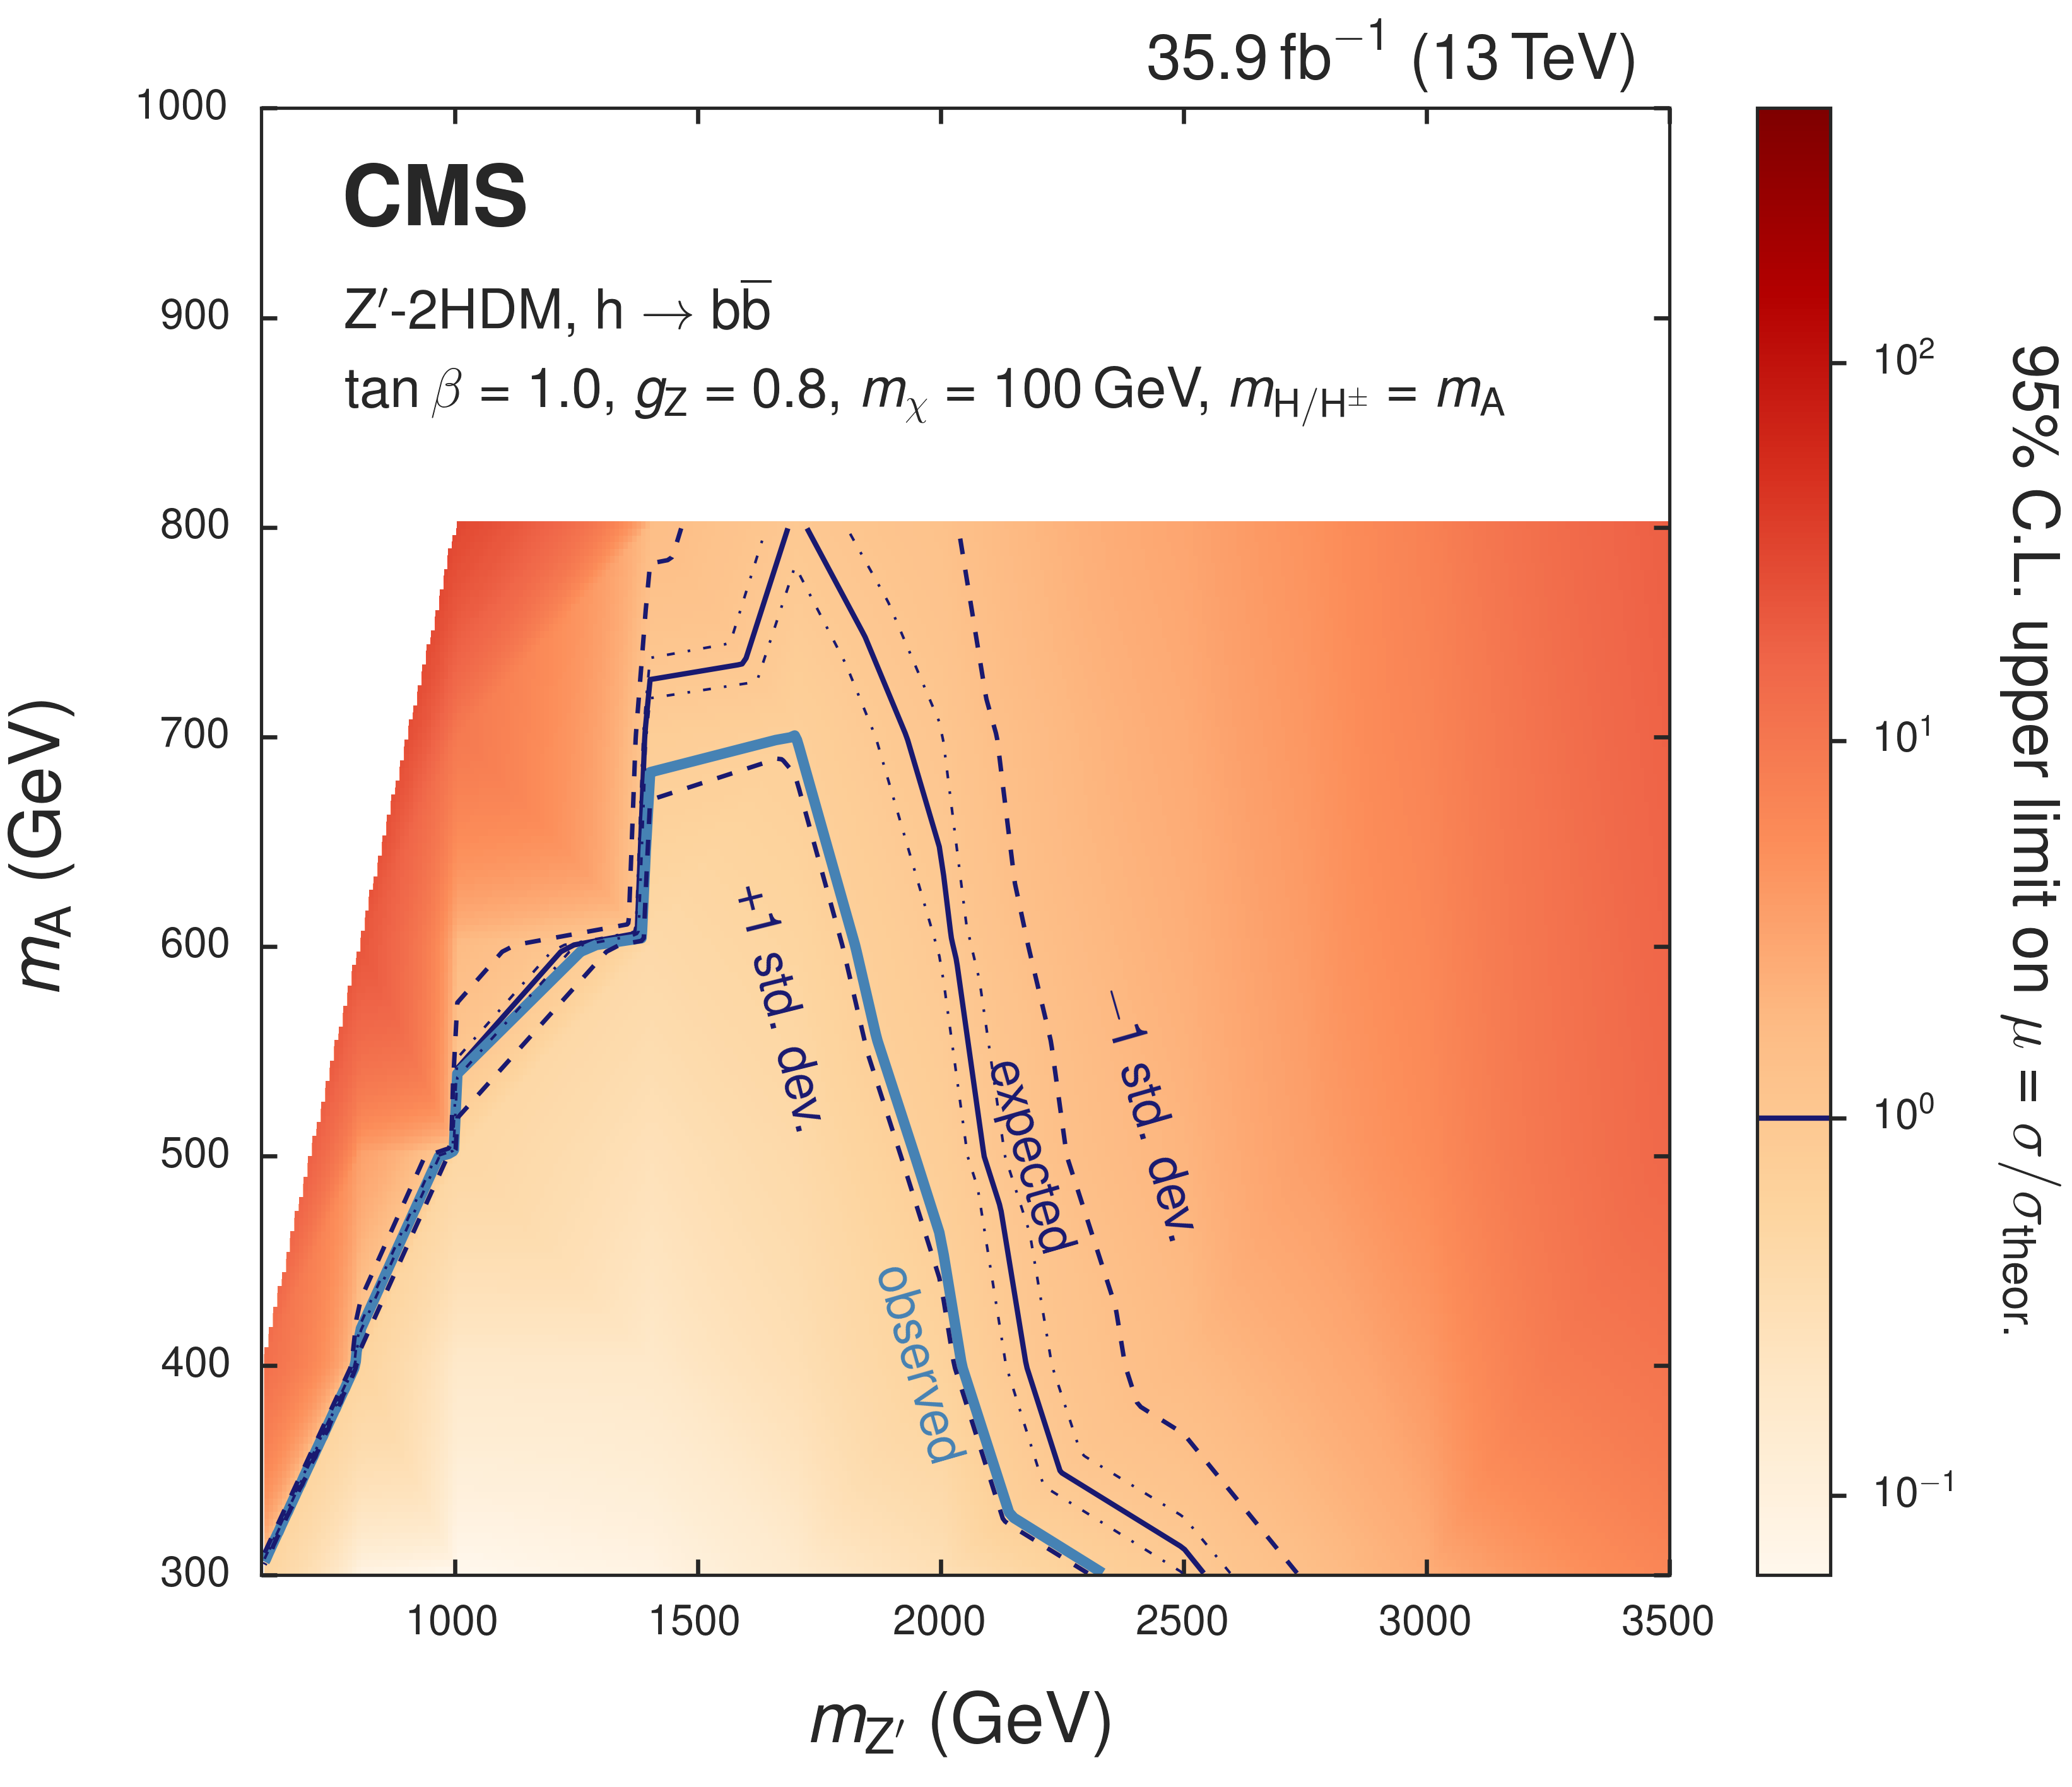
\includegraphics[width=0.475\textwidth]{figures/limits/limits_2hdm2d.png}
%  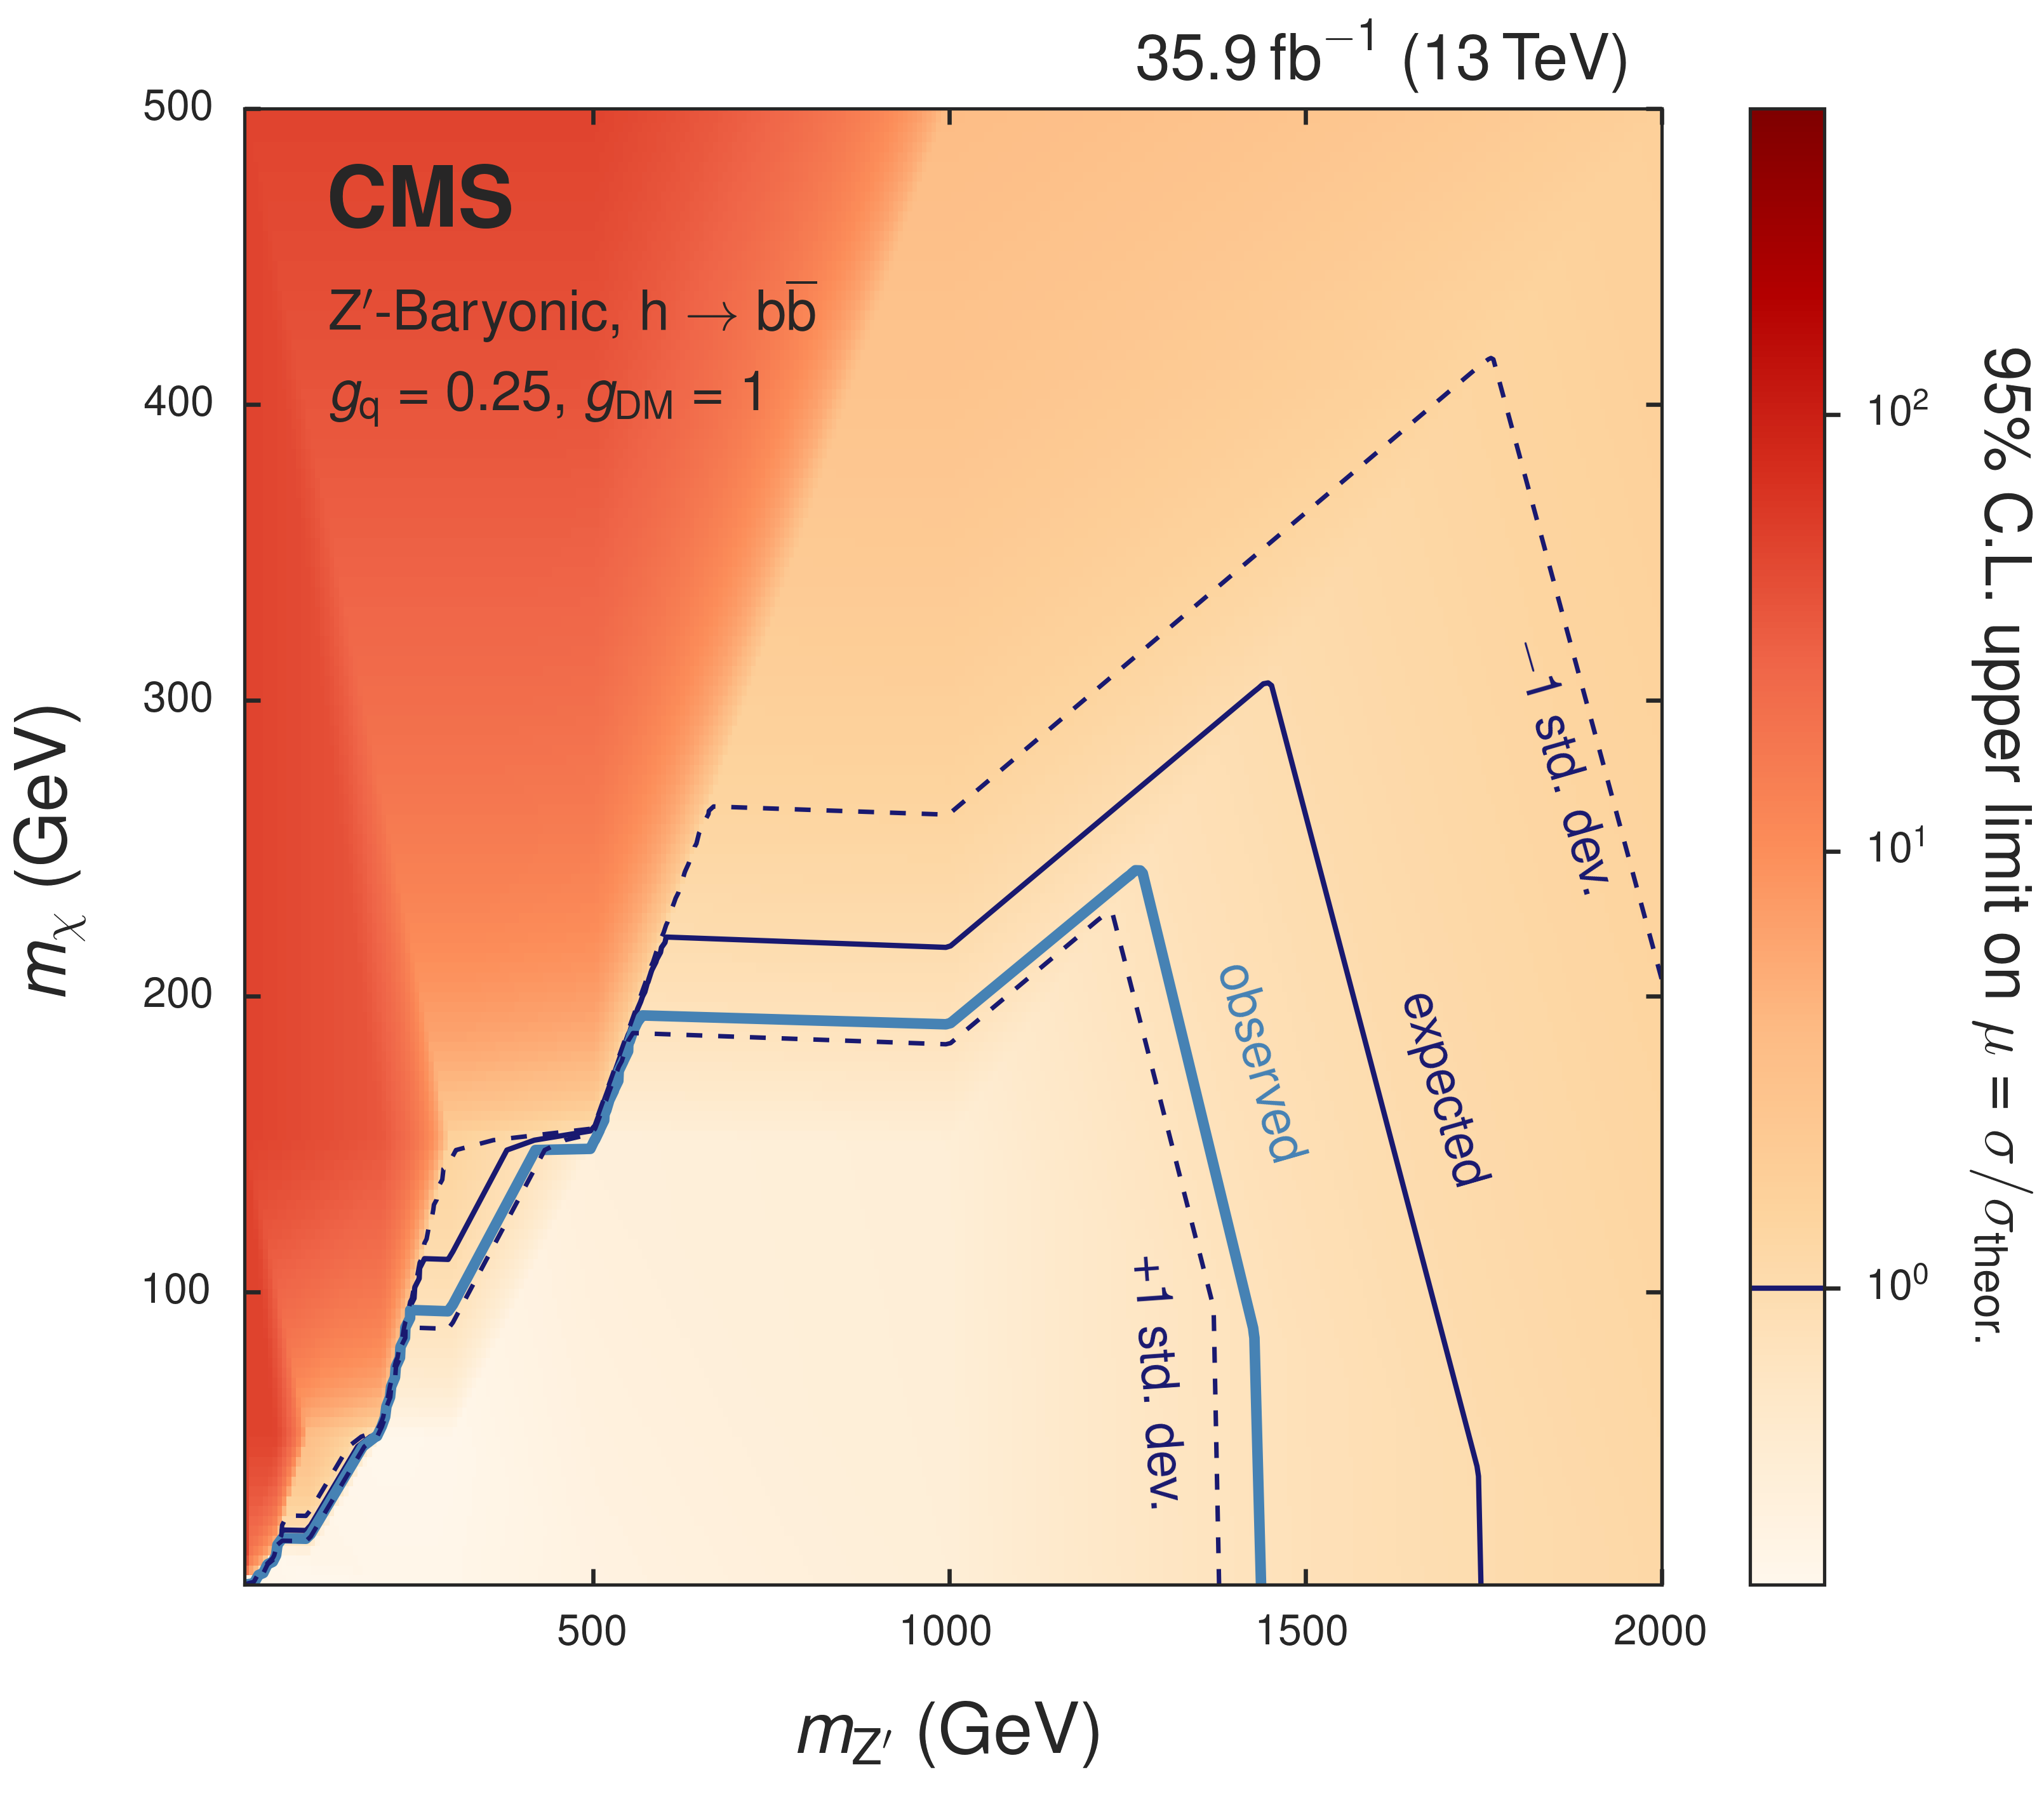
\includegraphics[width=0.475\textwidth]{figures/limits/limits_barzp2d.png}
  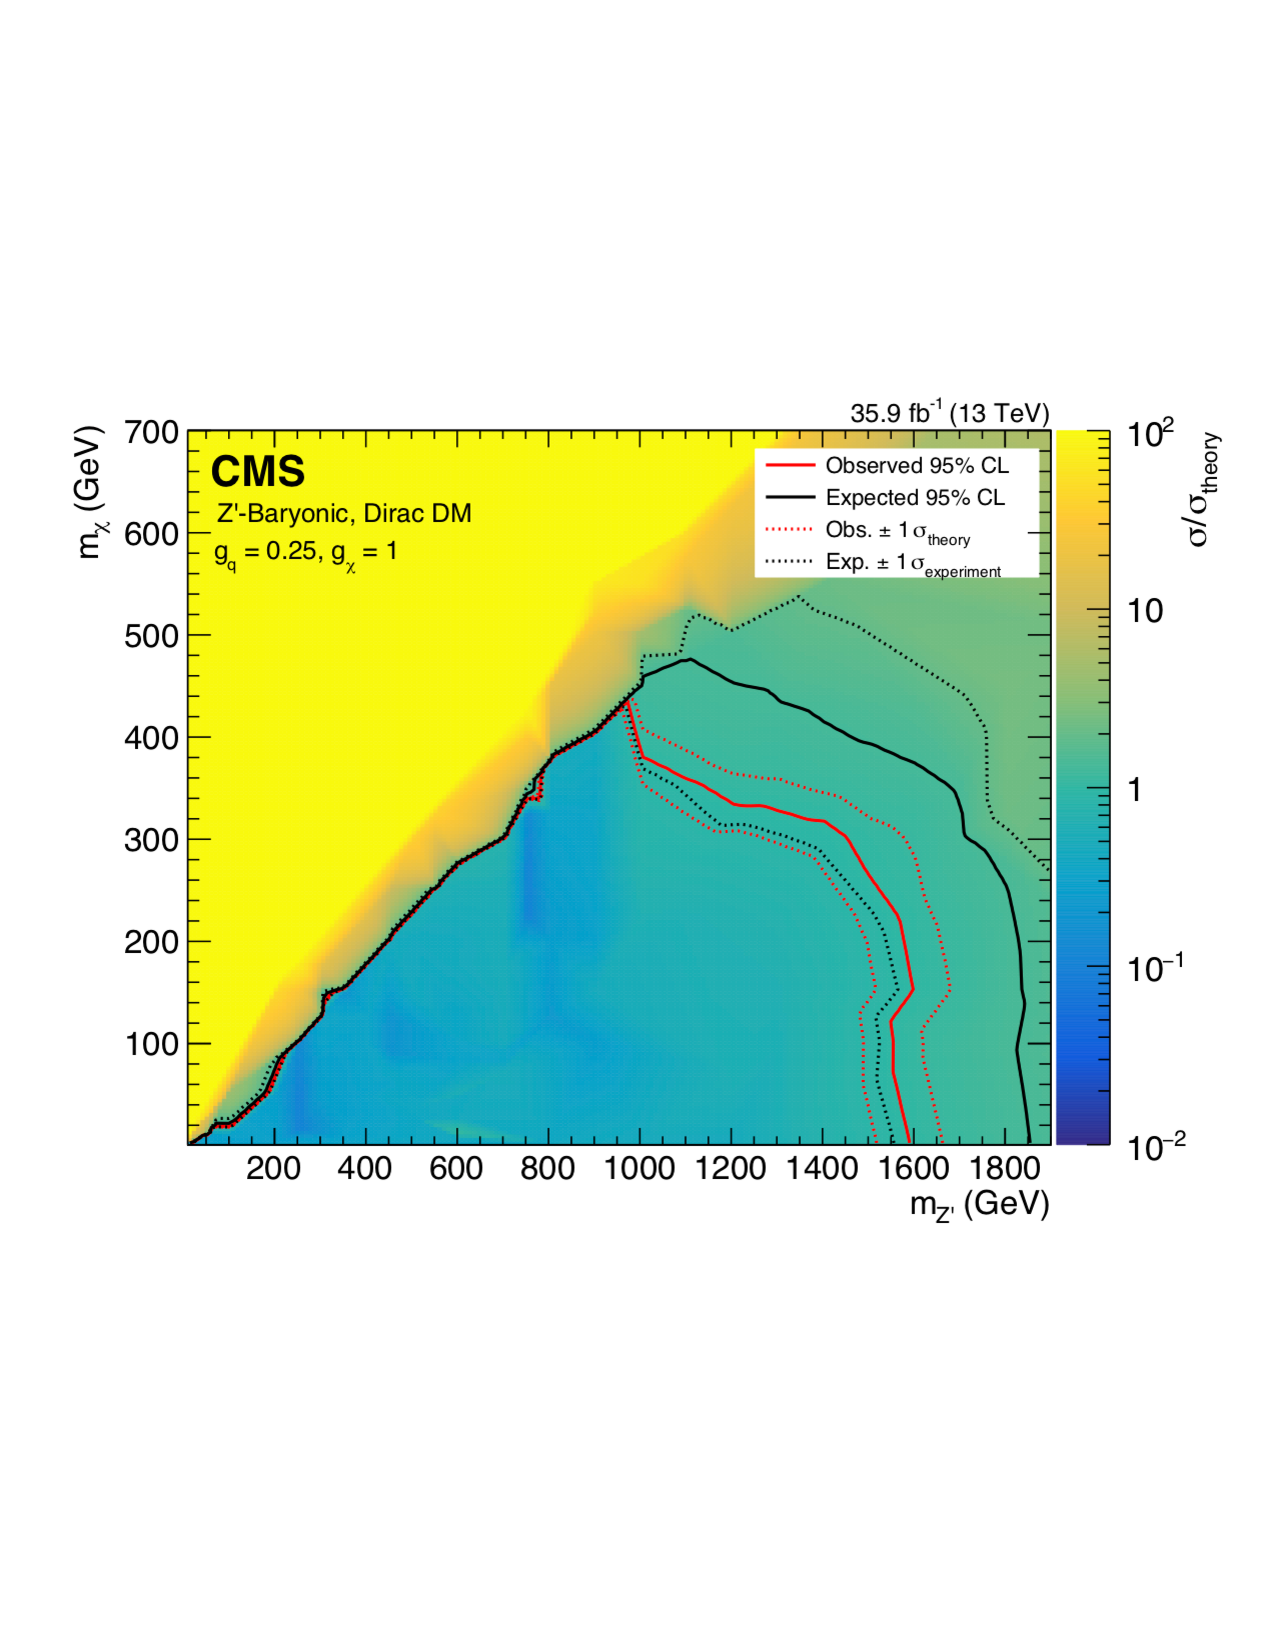
\includegraphics[width=0.475\textwidth]{figures/limits/limit2d_zpb_monohbb_.pdf}
  \caption{Upper limits on the signal strength modifier for the baryonic Z' model  as a function of $m_{Z'}$ and $m_\chi$. Mediators of up to 1.6\TeV are excluded for a DM mass of 1\GeV. Masses of the DM particle itself are excluded up to 430\GeV for a Z' mass of 1.25\TeV.}
  \label{fig:limits}
\end{figure}




Figure~\ref{fig:limits} shows the expected and observed exclusion range as a function of $m_{\text{Z}'}$ and $m_{\chi}$ for the baryonic Z' model. For a DM mass of 1\GeV, masses $\mzp<1.6\TeV$ are excluded. The expected exclusion boundary is 1.85\TeV. Masses for the DM particles of up to 430\GeV are excluded for a 1.1\TeV Z' mass. These are the most stringent limits on this model so far. %These results can be turned into limits on the spin-independent cross section, see $-$FIG XX$-$. 

To compare results with DM direct detection experiments, limits from the baryonic Z' model are presented in terms of a spin-independent (SI) cross section \SigSI for DM scattering off a nucleus.
Following the recommendation of Ref.~\cite{presentDM}, the value of $\sigma_\text{SI}$ is determined by the equation:

\begin{equation}
\sigma_\text{SI} = \frac{f^2(g_{\cPq})g^2_{\mathrm{DM}}\mu^2_{\mathrm{n}\chi}}{\pi m^4_{\mathrm{med}}},
\end{equation}

where $\mu_{\mathrm{n}\chi}$ is the reduced mass of the DM-nucleon system, $f(g_{\cPq})$ is the mediator-nucleon coupling, which is dependent on the mediator coupling to SM quarks $g_{\cPq}$, $g_{DM}$ is the mediator coupling to SM particles, and $m_{\text{med}}$ is the mass of the mediator.
The resulting \SigSI limits as a function of DM the mass are shown in Fig.~\ref{fig:limitsdd}.
%Exclusions from several direct detection experiments are compared to our result.
Under the assumptions made for the baryonic Z' model, these limits are the most stringent to date for $m_\chi < 5\GeV$.


\begin{figure}
  \centering
%  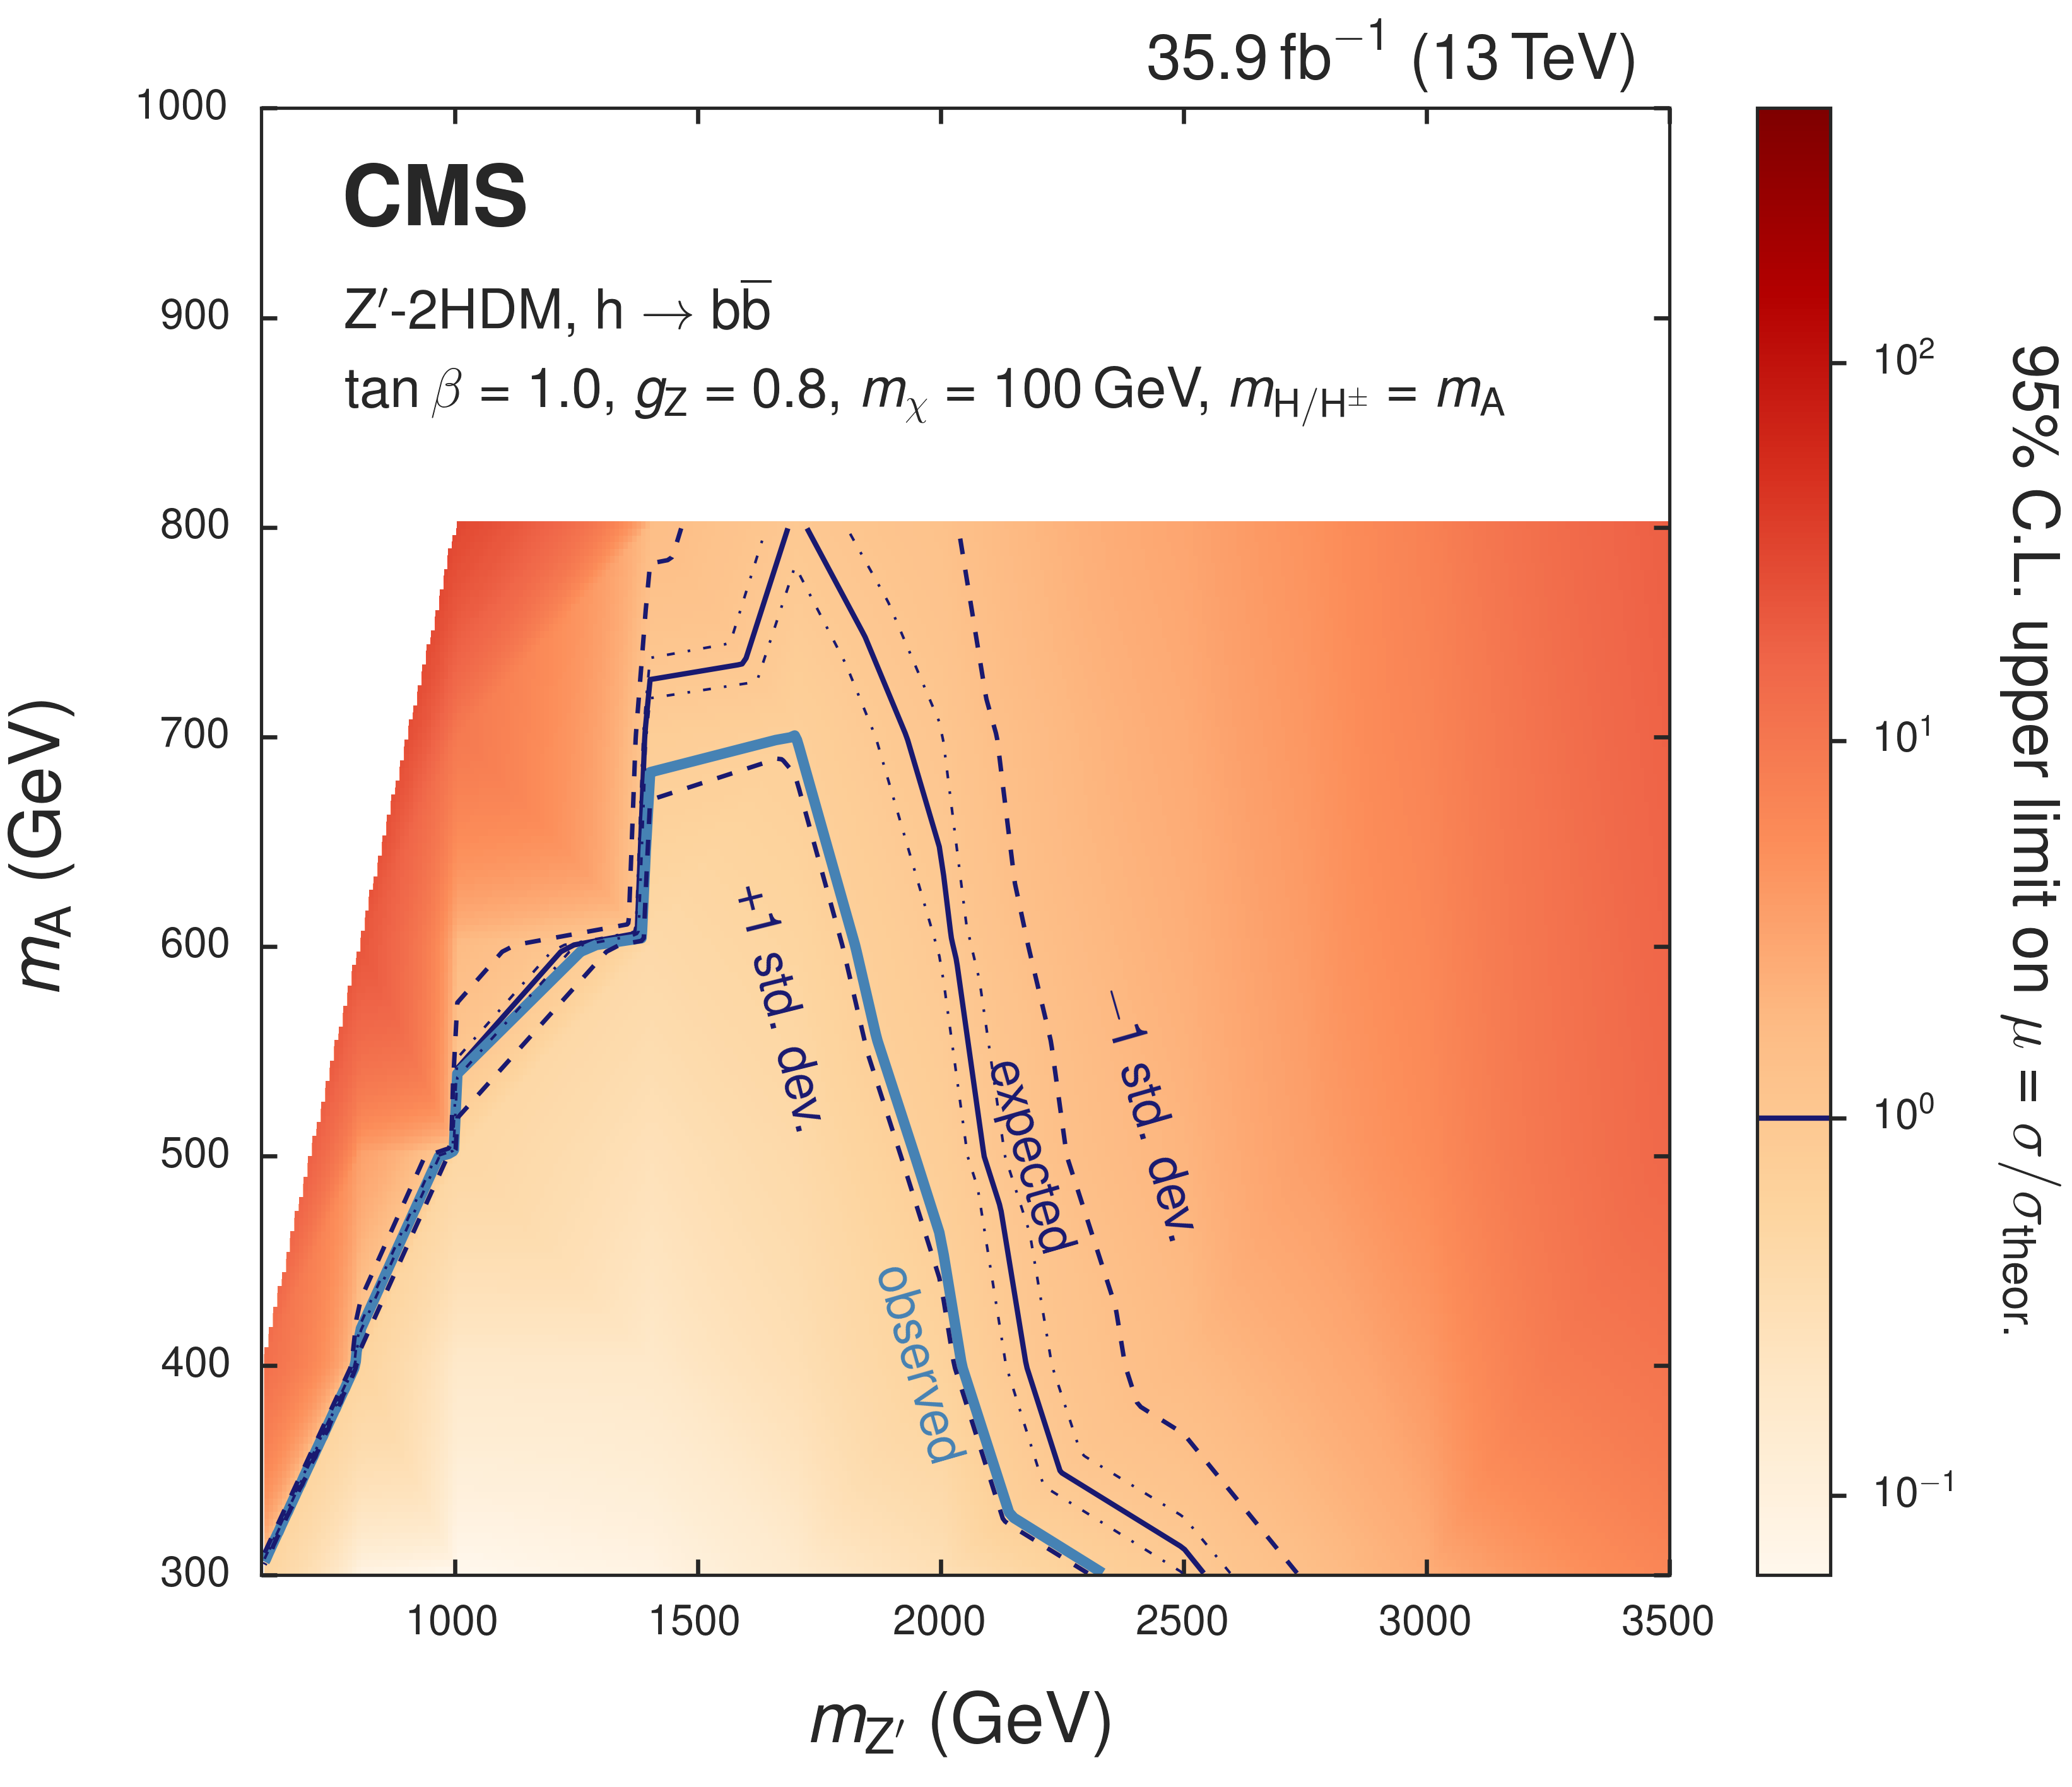
\includegraphics[width=0.475\textwidth]{figures/limits/limits_2hdm2d.png}
%  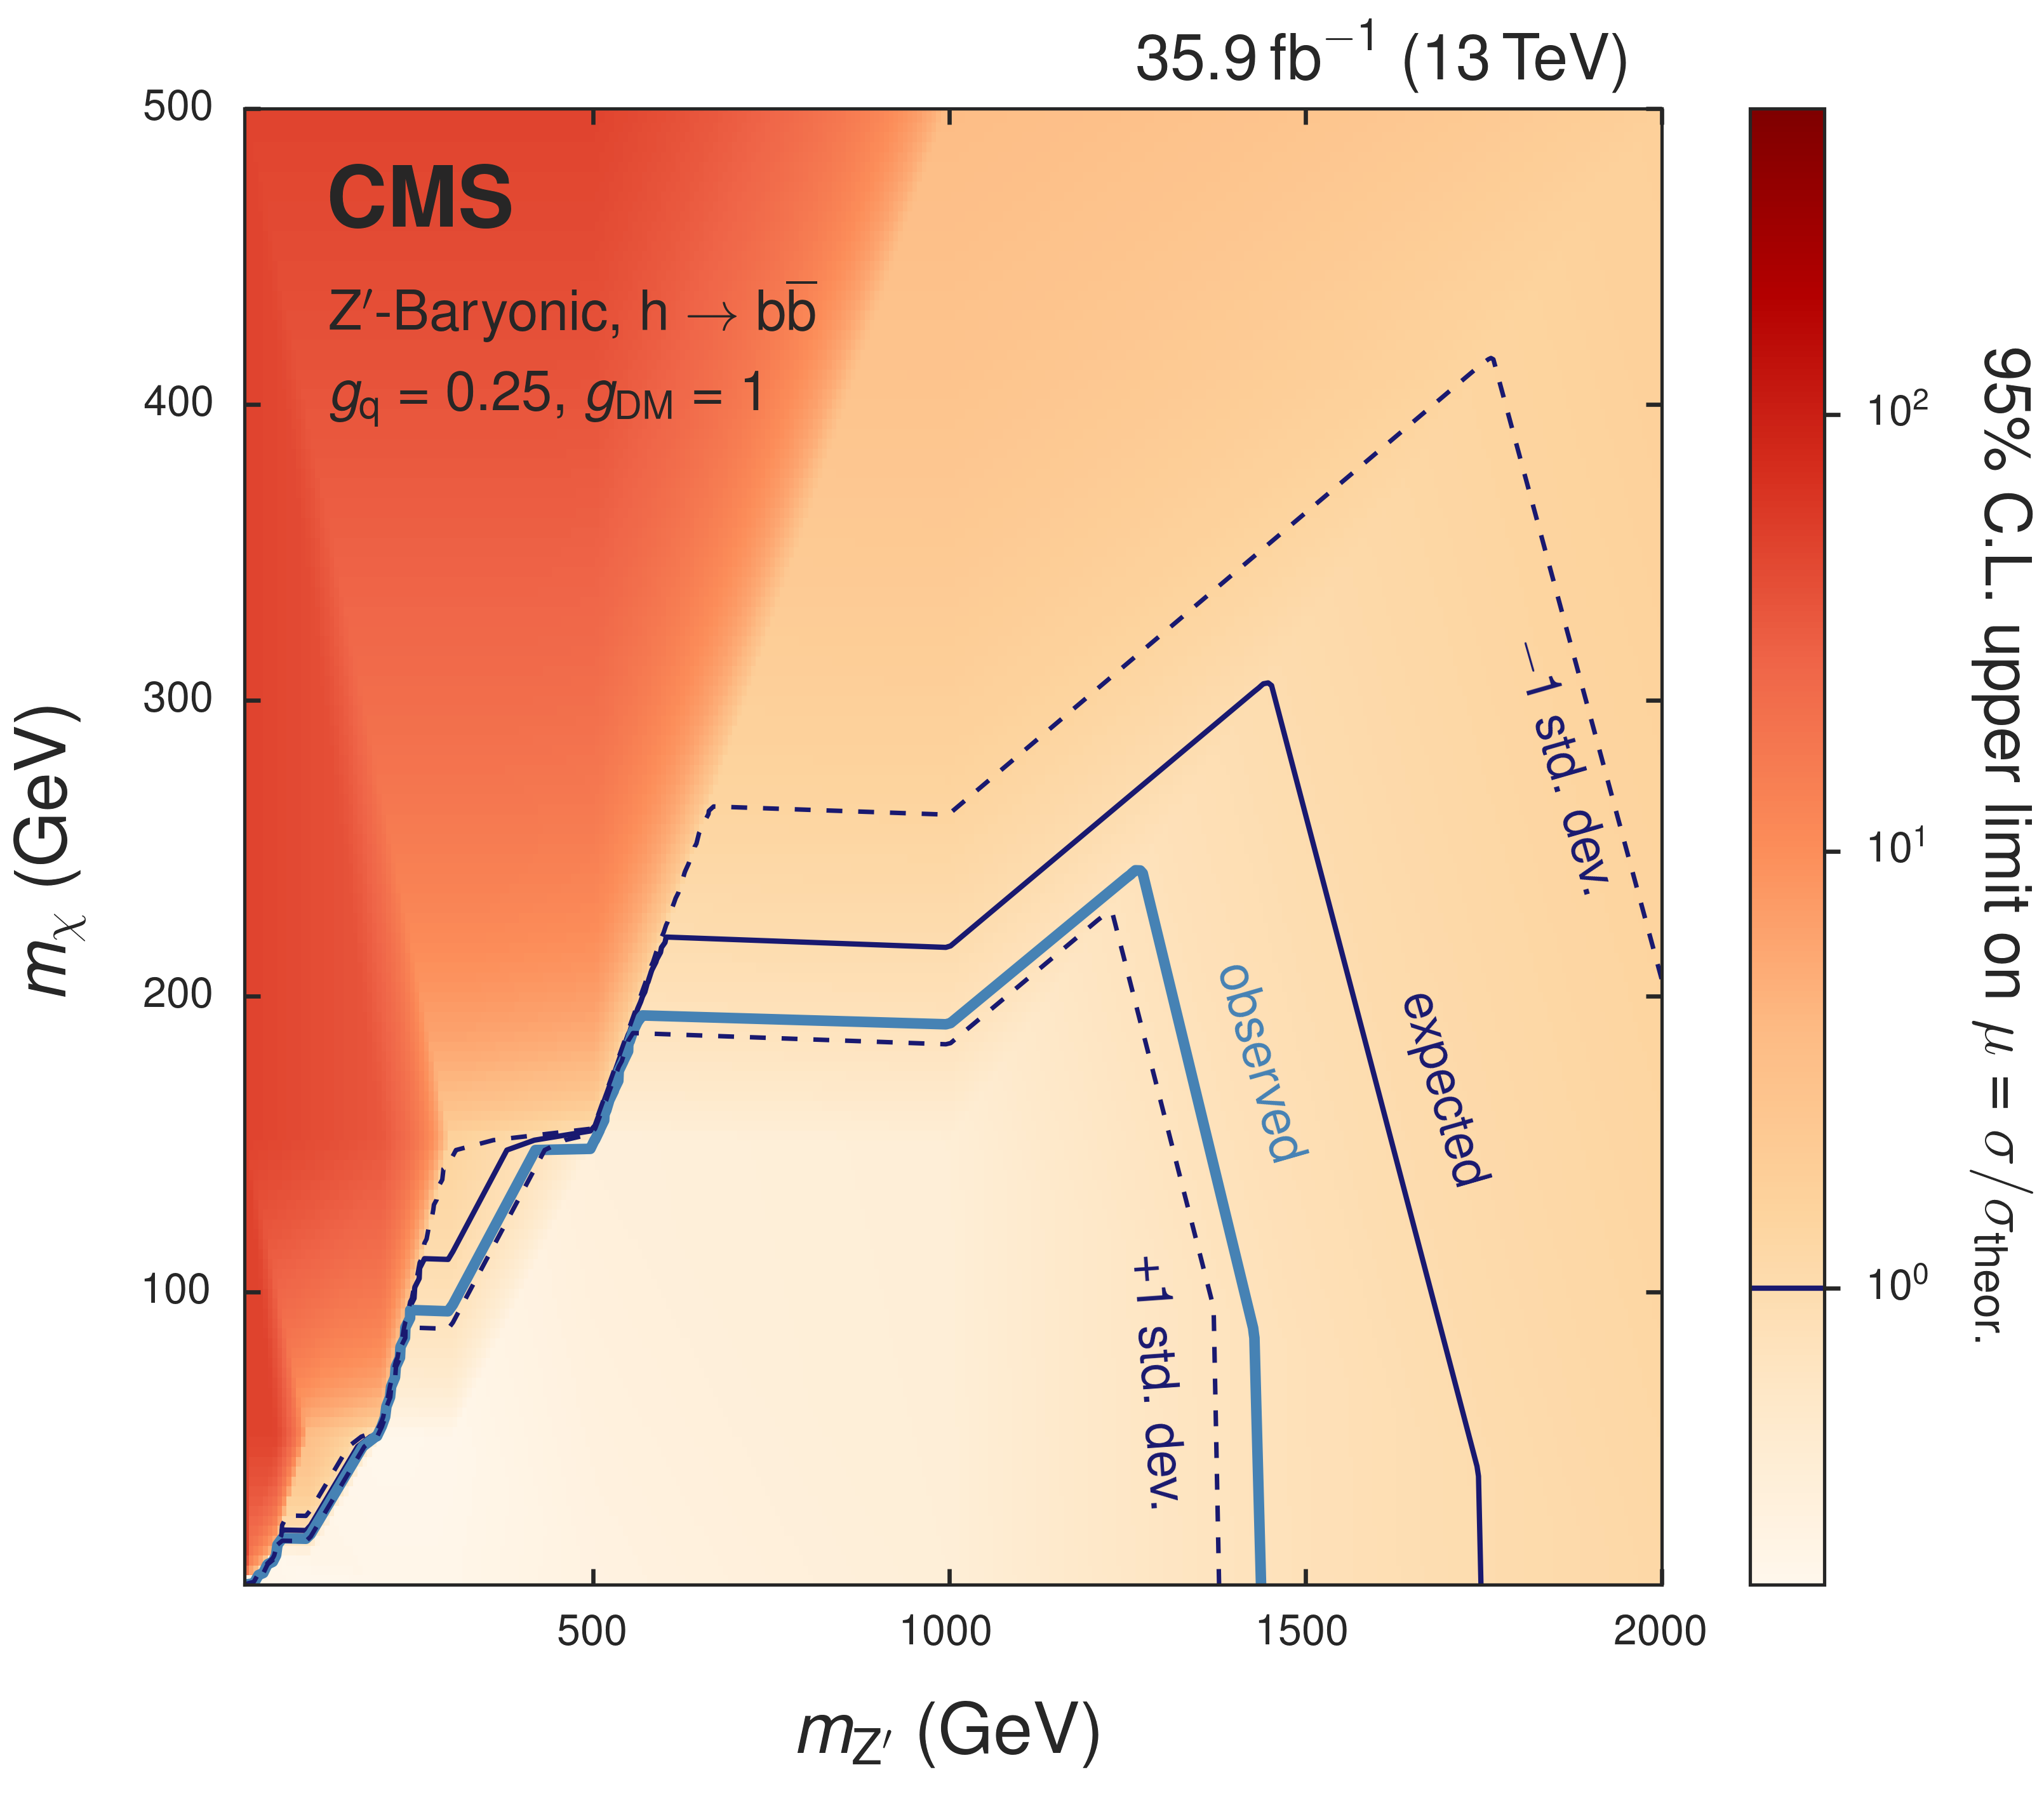
\includegraphics[width=0.475\textwidth]{figures/limits/limits_barzp2d.png}
  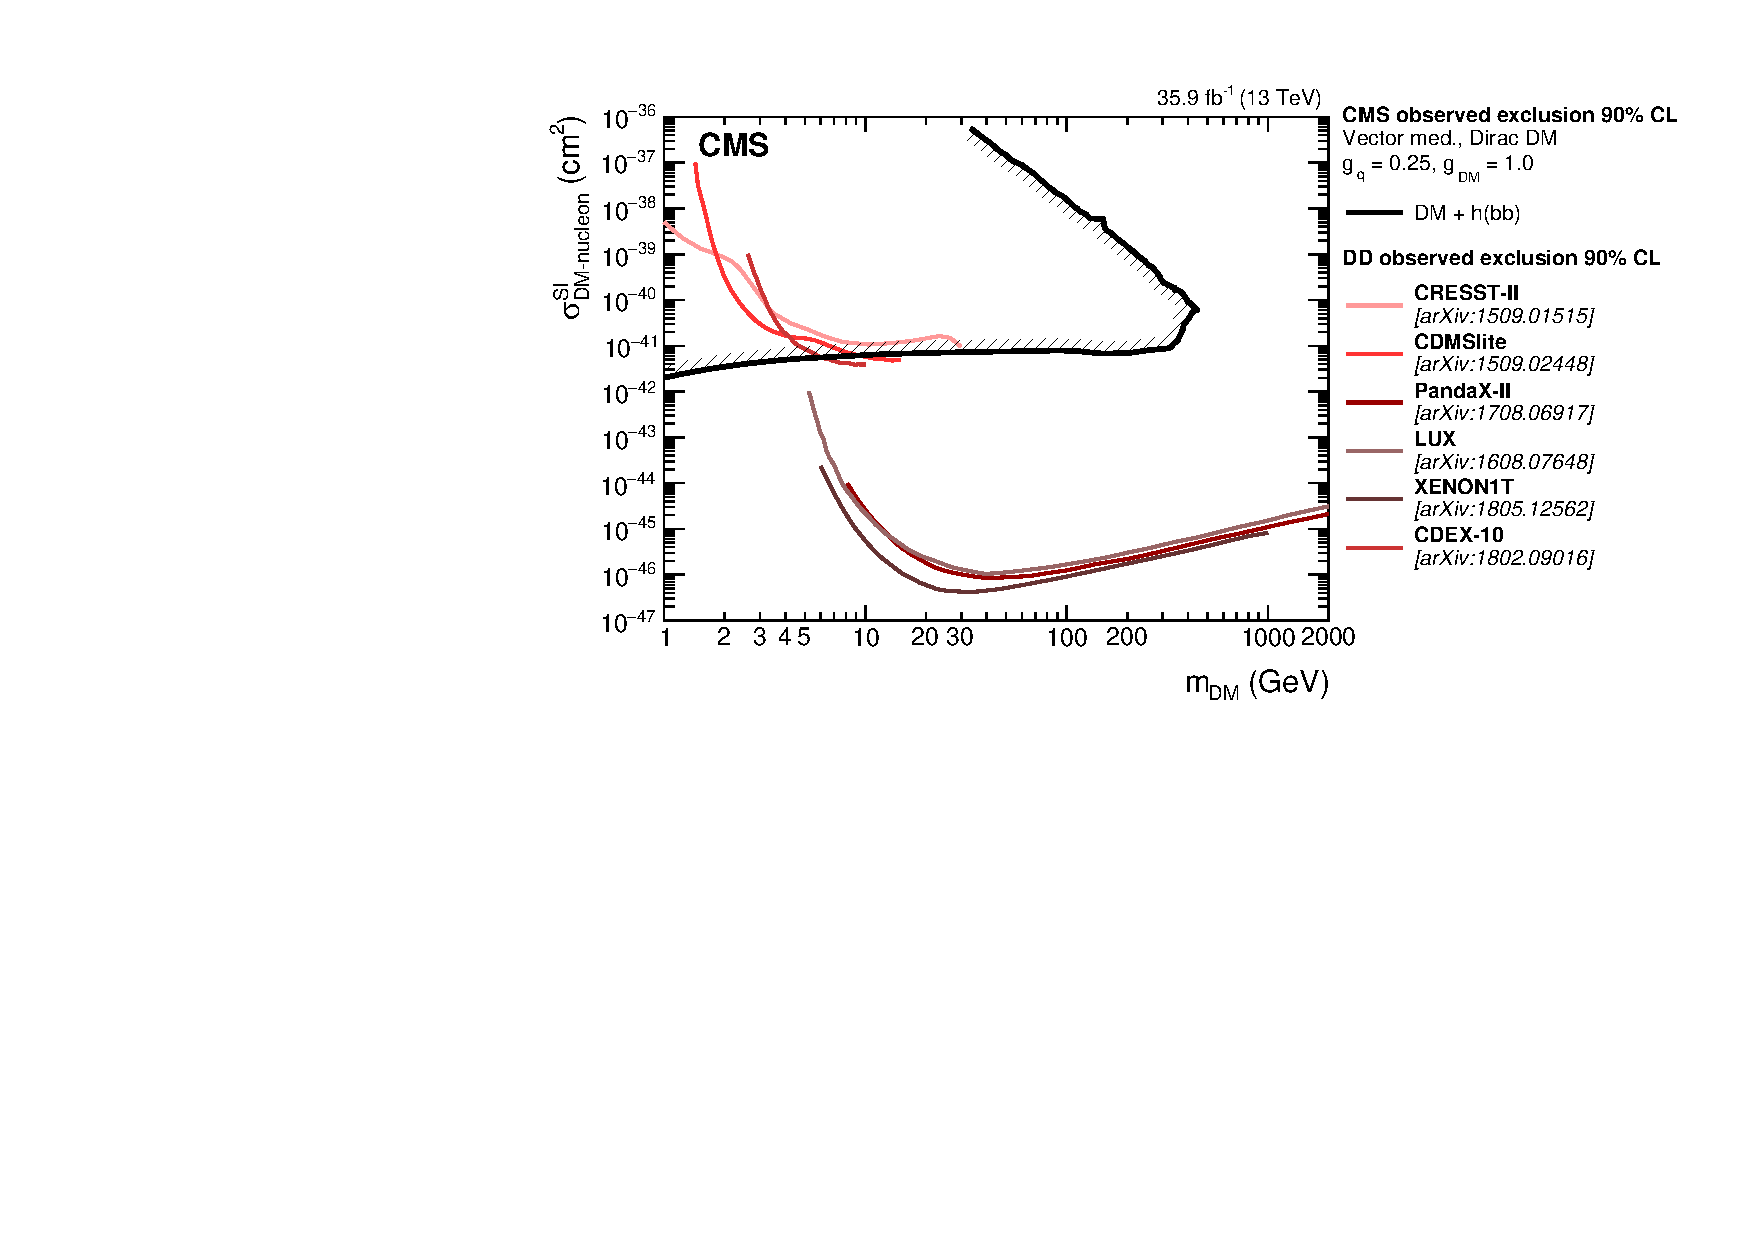
\includegraphics[width=0.775\textwidth]{figures/limits/SpinIndepend_XsecDM_MonoHbb_bb_obs_Summary.pdf}
  \caption{The 90\% \CL exclusion limits on the DM-nucleon SI scattering cross section as a function of $m_{\chi}$. 
Results on the baryonic Z' model obtained in this analysis are compared with those from a selection of direct detection (DD) experiments. 
The latter exclude the regions above the curves. 
Limits from CDMSLite~\cite{CDMSLite}, LUX~\cite{LUX}, XENON-1T~\cite{XENON1T}, PandaX-II~\cite{PandaxII}, and CRESST-II~\cite{CresstII} are shown.}
  \label{fig:limitsdd}
\end{figure}


\section{Summary}

A search for the associated production of dark matter (DM) particles with a Higgs
boson decaying into a pair of bottom quarks is presented. No significant
deviation from the predictions of the standard model (SM) is observed, and upper limits on
the production cross section predicted by a type-2 two Higgs doublet model
extended by an additional light pseudoscalar boson $a$ (2HDM+$a$) and the
baryonic Z' model are established. They constitute the most stringent collider exclusions placed on the parameters in these
models so far. For the nominal choice of the mixing angle $\sin\theta$
and $\tan\beta$ in the 2HDM+$a$ model, the search excludes masses
$500<m_A<900\GeV$ (where $A$ is the heavy pseudoscalar boson) assuming $m_a=150\GeV$. Scanning over
$\sin\theta$ with $\tan\beta$ = 1, we exclude
$0.35<\sin\theta<0.75$ for $m_\text{A}=600\GeV$ and
$m_\text{a}=200\GeV$.  Finally, $\tan\beta$ values between 0.5 and 2.0
(1.6) are excluded for $m_\text{A}=600\GeV$ and $m_\text{a}=100$
(150)\GeV and $\sin\theta$ $>$ 0.35. In all 2HDM+$a$ interpretations, a DM mass of $m_\chi=10\GeV$ is assumed. For the baryonic Z' model, we exclude Z' boson masses up to 1.6\TeV for a DM mass of 1\GeV, and DM masses up to 430\GeV for a Z' boson mass of 1.1\TeV. The reinterpretation of the results for the baryonic Z' model in terms of an SI nucleon scattering cross section yields a higher sensitivity for $m_\chi<5\GeV$ than existing results from direct detection experiments, under the assumptions imposed by the model. The 2HDM+$a$ model is probed experimentally for the first time.

 

%

Table \ref{tab:eventYieldTable} shows, for the \Hbb channel, the 
SR post-fit yields for each background and signal mass point along with the 
sum of the statistical and systematic uncertainties for the resolved and boosted regimes. 

For the \HGG channel, when applying the event selection to the data, two events are observed in the $m_{\gamma\gamma}$ sidebands and are used to 
evaluate the magnitude of the nonresonant background as described in Section~\ref{sec:bkg_model}. 
This yields an expected number of $0.38 \pm 0.27 (stat)$ nonresonant background events in the SR.
Expected resonant background contributions are taken from the simulation as detailed in Section~\ref{sec:bkg_model} and are $0.057 \pm 0.006 (stat)$ events considering both the Vh production (dominant) and the gluon fusion mode. Zero events are observed in the SR in the data.



Since no excess of events has been observed over the SM background expectation in the signal region, the results of this search are interpreted in terms of an upper limit on the production cross 
section of DM candidates in association with a Higgs boson via $\PZpr \rightarrow \Az \Ph \rightarrow \chi \bar{\chi} \PAQb\PQb(\gamma\gamma)$. 
The upper limits are computed at 95\% confidence level (CL) using a modified frequentist method (CL$_s$) \cite{yellowReport, bib:CLS1, bib:CLS2} computed with an asymptotic approximation \cite{bib:CLS3}. 
A profile likelihood ratio is used as the test statistic in which systematic uncertainties are modeled as nuisance parameters.
These limits are obtained as a function of \mzp and \maz for both Higgs boson decay channels and for the combination of the two. The two decay channels are combined using the branching ratios predicted by the SM.
In the combination of the two analyses, all signal and \MET-related systematic uncertainties as well as the systematic uncertainty on the integrated luminosity 
are assumed to be fully correlated.

Figure~\ref{fig:limitsexpected} (left) shows the 95\% CL expected and observed limits on the dark matter production cross section for 
\Hbb and \HGG for \maz = 300 GeV. 
Figures~\ref{fig:limitsexpected} (right) and~\ref{fig:limit2d} show the 95\% CL  expected and observed upper limits on the signal strength. 
For \maz = 300 GeV, the \mzp mass range 600 to 1780 \GeV is expected to be excluded with a 95\% CL when the signal model 
cross section is calculated using \gzp = 0.8. 
The observed data excludes, for \maz = 300 \GeV the \zp mass range of 600 to 1860 GeV. 
When the signal model cross section is calculated using the constrained \gzp, the expected exclusion range is 830 to 1890 GeV, 
and with the observed data the exclusion range is 770 to 2040 GeV. 



\begin{acknowledgments}
We congratulate our colleagues in the CERN accelerator departments for the excellent performance of the LHC and thank the technical and administrative staffs at CERN and at other CMS institutes for their contributions to the success of the CMS effort. In addition, we gratefully acknowledge the computing centers and personnel of the Worldwide LHC Computing Grid for delivering so effectively the computing infrastructure essential to our analyses. Finally, we acknowledge the enduring support for the construction and operation of the LHC and the CMS detector provided by the following funding agencies: BMWFW and FWF (Austria); FNRS and FWO (Belgium); CNPq, CAPES, FAPERJ, and FAPESP (Brazil); MES (Bulgaria); CERN; CAS, MoST, and NSFC (China); COLCIENCIAS (Colombia); MSES and CSF (Croatia); RPF (Cyprus); SENESCYT (Ecuador); MoER, ERC IUT, and ERDF (Estonia); Academy of Finland, MEC, and HIP (Finland); CEA and CNRS/IN2P3 (France); BMBF, DFG, and HGF (Germany); GSRT (Greece); OTKA and NIH (Hungary); DAE and DST (India); IPM (Iran); SFI (Ireland); INFN (Italy); MSIP and NRF (Republic of Korea); LAS (Lithuania); MOE and UM (Malaysia); BUAP, CINVESTAV, CONACYT, LNS, SEP, and UASLP-FAI (Mexico); MBIE (New Zealand); PAEC (Pakistan); MSHE and NSC (Poland); FCT (Portugal); JINR (Dubna); MON, RosAtom, RAS, RFBR and RAEP (Russia); MESTD (Serbia); SEIDI, CPAN, PCTI and FEDER (Spain); Swiss Funding Agencies (Switzerland); MST (Taipei); ThEPCenter, IPST, STAR, and NSTDA (Thailand); TUBITAK and TAEK (Turkey); NASU and SFFR (Ukraine); STFC (United Kingdom); DOE and NSF (USA).

\hyphenation{Rachada-pisek} Individuals have received support from the Marie-Curie program and the European Research Council and Horizon 2020 Grant, contract No. 675440 (European Union); the Leventis Foundation; the A. P. Sloan Foundation; the Alexander von Humboldt Foundation; the Belgian Federal Science Policy Office; the Fonds pour la Formation \`a la Recherche dans l'Industrie et dans l'Agriculture (FRIA-Belgium); the Agentschap voor Innovatie door Wetenschap en Technologie (IWT-Belgium); the Ministry of Education, Youth and Sports (MEYS) of the Czech Republic; the Council of Science and Industrial Research, India; the HOMING PLUS program of the Foundation for Polish Science, cofinanced from European Union, Regional Development Fund, the Mobility Plus program of the Ministry of Science and Higher Education, the National Science Center (Poland), contracts Harmonia 2014/14/M/ST2/00428, Opus 2014/13/B/ST2/02543, 2014/15/B/ST2/03998, and 2015/19/B/ST2/02861, Sonata-bis 2012/07/E/ST2/01406; the National Priorities Research Program by Qatar National Research Fund; the Programa Severo Ochoa del Principado de Asturias; the Thalis and Aristeia programs cofinanced by EU-ESF and the Greek NSRF; the Rachadapisek Sompot Fund for Postdoctoral Fellowship, Chulalongkorn University and the Chulalongkorn Academic into Its 2nd Century Project Advancement Project (Thailand); the Welch Foundation, contract C-1845; and the Weston Havens Foundation (USA).
\end{acknowledgments}


%\input{dataAndSimulation.tex}
%
%A global event reconstruction is performed using the particle-flow (PF) \cite{CMS-PAS-PFT-09-001, ParticleFlow} algorithm.
%, which optimally combines the information from all subdetectors and 
%produces a list of stable particles (muons, electrons, photons, 
%charged and neutral hadrons). 


\section{Event reconstruction}

The reconstructed interaction vertex with the largest value of $\sum_{i} p_\mathrm{T}^{i2}$, where $p_\mathrm{T}^{i}$ is the transverse momentum of the $i^\mathrm{th}$ track 
associated with the vertex, is selected as the primary event vertex. The offline selection requires all events to have at least one primary vertex reconstructed within a 24\,cm window along the z-axis around the nominal interaction point, and a transverse distance from the nominal interaction region less than 2\,cm.

The particle-flow (PF) \cite{Sirunyan:2017ulk} algorithm aims to reconstruct all the physics objects described in this section. At large Lorentz boosts, the two b quarks from the Higgs boson decay may produce jets that overlap and make their individual reconstruction difficult. In this search, large-area jets clustered from PF candidates using the Cambridge--Aachen algorithm~\cite{cajets} with a distance parameter of $1.5$ (CA15 jets) are utilized to identify the Higgs boson candidate.  The large cone size is chosen in order to include events characterized by the presence of Higgs bosons with medium boost ($p_\mathrm{T}$ of the order of 200 GeV).
To reduce the impact of particles arising from pileup interactions,  the four-vector of each PF candidate is scaled with a weight calculated with the pileup per particle identification (PUPPI) algorithm ~\cite{puppi} prior to the clustering.
The absolute jet energy scale is corrected using calibrations derived from data~\cite{jec}. The CA15 jets are also required to be central ($\eta$ $<$ 2.4).
The ``soft-drop'' (SM) jet grooming algorithm~\cite{msd} is applied to remove soft wide-angle radiation from the jets. We refer to the groomed mass of the CA15 jet as $m_\text{SD}$. 

The ability to identify two b quarks inside a single CA15 jet is
crucial for this search. A likelihood for the CA15 jet to contain two
b quarks is derived by combining the information from primary and secondary vertices and tracks in a multivariate discriminant optimized to distinguish the Higgs to \bb decays from energetic quarks or gluons~\cite{Sirunyan:2017ezt} that appear inside the CA15 jet cone.
%The chosen working point of double b-tagger ($>$ 0.75) corresponds to the same background efficiency of the medium 
%working point of minimum of the CSV score of subjets. 
The working point chosen for this algorithm (the ``double-b tagger'')
corresponds to an identification efficiency of 50\% for a \bb system
with a \pt of 200 GeV, and a probability of about 10-13\% for
misidentifying CA15 jets originating from other combinations of quarks
or gluons. The efficiency of the algorithm increases with the \pt~of the \bb system.

%These numbers have been determined in simulation samples with at least one reconstructed CA15 jet with $\pt>200$\GeV and an otherwise inclusive selection. 

Energy correlation functions are used to identify the two-prong
structure in the CA15 jet expected from a Higgs boson decay to two b
quarks. The energy correlation functions are sensitive to correlations among the constituents
of CA15 jets (the PF candidates)~\cite{ecf}. They are $N$-point correlation functions ($e_N$) of the constituents' momenta, weighted by the angular separation of the constituents.
%Discriminating variables are constructed by using ratios of these functions.
%\begin{linenomath}
%\begin{equation}
%  \frac{_ae_N^\alpha}{(_be_M^\beta)^x}, \text{ where $M\leq N$ and $x= \frac{a\alpha}{b\beta}$}.
%  \label{eq:ecf}
%\end{equation}
%\end{linenomath}
%                                                                                                                                                                                                
%In Eq.~(\ref{eq:ecf}), the six free parameters are
%$N,a,\alpha,M,b,~\mathrm{and}~\beta$ and the value of $x$ is chosen to
%make the ratio dimensionless. An $N$-pronged jet is expected to have
%$e_N \gg e_M$ for $M>N$. 
As motivated in Ref.~\cite{ecf}, the ratio $N_2 =
e_3^{(\beta)}/(e_2^{(\beta)})^2$ is proposed as a two-prong tagger for
the identification of the CA15 jet containing the Higgs boson decay
products; the parameter $\beta$, which controls the weighting of the angles between constituent pairs in the computation of
the $N_2$ variable, is chosen to be 1 as the value that gives the best two-prong jet reconstruction. 

%\begin{equation}
%  N_2(\beta) = \frac{e(2,3,\beta)}{e(1,2,\beta)^2}
%\end{equation}

%When computing the $N_2$ variable, only the first one hundred highest $p_T$ constituents that survive soft-drop grooming are used.

It is noted that requiring a jet to be two-pronged by using a jet substructure variable,
such as $N_2$, will affect the shape of the distribution of $m_\text{SD}$ for the
background processes. In this search, the value of $m_\text{SD}$ is required to be consistent with the Higgs boson mass.
It is therefore desirable to preserve a smoothly falling jet mass
distribution as a function of \pt as the one expected for QCD-like jets (i.e., jets that
do not originate from a heavy resonance decay). 
As motivated in Ref.~\cite{ddt}, the stability of $N_2$ is tested against the variable
$\rho=\ln(m_{\text{SD}}^2/\pt^2)$, since the distribution of $\rho$ is expected to be stable in QCD-like jets.
%: since the jet mass distribution for QCD multijet
%events is expected to scale with \pt, decorrelating the $N_2$ variable
%as a function of $\rho$ and \pt would be the most appropriate procedure. 
The decorrelation strategy described in Ref.~\cite{ddt} is applied,
choosing a background efficiency of 20\%, which corresponds to a
signal efficiency of roughly 50\%. This results in a modified tagging
variable, which we denote as $N_2^\text{DDT}$, where the superscrit DDT stands for designing decorrelated taggers~\cite{ddt}. Fig.~\ref{n2ddt} shows the expected distribution of the the $N_2^\text{DDT}$ for CA15 jets matched to a Higgs boson decaying to a $b\bar{b}$ pair, together with the distributions expected for CA15 jets matched to hadronically decaying top quarks and for QCD-like CA15 jets.
%This choice of background (or, equivalently, signal) efficiency has been optimized in order to maximize the $S/B$ ratio while retaining high enough event yield for the data-driven estimation of the background processes.
\begin{figure}
\centering
  \includegraphics[width=0.65\textwidth]{figures/ddt_N2DDT_ns.pdf} \\
\caption{The $N_2^\text{DDT}$ distribution as expected for CA15 jets matched to a Higgs boson decaying to a $b\bar{b}$ pair (in red), compared to the expected distribution for CA15 matched to the decay products of top quarks decaying hadronically (in grey). The distribution corresponding to CA15 jets that do not originate from a heavy resonance decay is also shown in blue.}
\label{n2ddt}
\end{figure}


This search also utilizes narrow jets clustered
with the anti-$\kt$ algorithm~\cite{Cacciari:2008gp}, with a distance
parameter of $0.4$ (“AK4” jets). Narrow jets originating from b quarks are identified using the combined secondary vertex (CSVv2) algorithm \cite{Sirunyan:2017ezt}. The working point used in this search has a b jet identification efficiency of 81\%, a charm jet selection efficiency of 37\%, and a 9\% probability of misidentifying light-flavor jets~\cite{Sirunyan:2017ezt}. Jets that are b tagged are required to be central ($|\eta|<2.4$).
%%An event with any additional narrow jet passing the loose b tagging requirement is vetoed to reduce the number of events containing top quarks. 

Electron reconstruction requires the matching of a supercluster in the ECAL with a track in the silicon tracker.
Identification criteria~\cite{Khachatryan:2015hwa} based on the ECAL shower shape and the consistency with originating from the primary vertex are imposed. The reconstructed electron is required to be within $|\eta|< 2.5$, excluding the transition region $1.44<|\eta|<1.57$ between the ECAL barrel and endcap. Muons candidates are selected by two different reconstruction approaches~\cite{CMSMuonJINST}: the one in which tracks in the silicon tracker are matched to a track
 segment in the muon detector, and the other one in which a track
 fit spanning the silicon tracker and muon detector is performed
 starting with track segments in the muon detector. Candidates that are found by both the approaches are considered as single candidates.
Further identification criteria are imposed on muon candidates to reduce the number of misidentified hadrons and poorly measured mesons tagged as muons~\cite{CMSMuonJINST}. 
These additional criteria include requirements on the number of hits in the tracker and in the muon systems, the fit quality of the global muon track, and its consistency with the primary vertex.
Muon candidates with $|\eta|< 2.4$ are considered in this analysis. 
With electron and muon candidates, the minimum \pt is required to be 10\GeV. Isolation is required for both the objects.
Hadronically decaying $\tau$ leptons, $\tau_\mathrm{h}$, are reconstructed using the hadron-plus-strips
  algorithm~\cite{CMSTauJINST}, which uses the charged hadron and neutral electromagnetic objects 
to reconstruct intermediate resonances into which the $\tau$ lepton decays. The $\tau_\mathrm{h}$
candidates with $\pt>18\GeV$ and $|\eta|< 2.3$ are considered~\cite{Khachatryan:2015hwa,Chatrchyan:2013sba,CMSTauJINST}. Photon candidates, identified by means of requirements on the ECAL energy distribution and its distance to the closest track, must have $\pt>15\GeV$ and $|\eta|< 2.5$. %We veto both $\tau_\mathrm{h}$ candidates and photon candidates in the search presented. %Events containing an isolated electron, muon, or an isolated hadronic tau passing these criteria are 

The missing transverse momentum $\vec{p}_{\mathrm{T}}^{\mathrm{miss}}$ is defined as the negative vectorial sum of the \pt of all the reconstructed PF candidates. Its magnitude is denoted as \MET. Corrections to jet momenta are propagated to the \MET calculation as well as event filters \cite{CMS-PAS-JME-16-004} are used to remove spurious high \MET events caused by instrumental noise in the calorimeters or beam halo muons~\cite{CMS-PAS-JME-16-004}. The filters remove about 1\% of signal events.

%For the control regions involving lepton(s) in the final state, the hadronic recoil against the boson is computed by removing the \pt of the lepton(s) from the \MET computation. The recoil is given by: 
%\begin{equation} 
%\vec{U}  = \MET + p_{\mathrm{T}}^{\ell,\ell\ell} 
%\end{equation} 
%where the \pt$^{l}$ is \pt of lepton(s) in the W (Z) control regions. 

%\section{Event selection}


Signal events are characterized by a high value of \MET, no isolated leptons or photons, and a CA15 jet identified as a Higgs boson candidate. In the signal region (SR) described
below, the dominant background contributions arise from Z+jets,
W+jets, and \ttbar production. To predict the \ptmiss~spectra of these
processes in the SR, data from different control regions (CRs) are used. Single-lepton CRs are designed to predict the \ttbar and W+jets backgrounds, while dilepton CRs predict the Z+jets background contribution. The hadronic recoil, $U$, defined by removing the \pt of the lepton(s) from the \MET computation in CRs, is used as a proxy for the \MET distribution of the main background processes in the SR. Predictions for other backgrounds are obtained from simulation.

A common set of preselection criteria is used for all regions. The presence of exactly one CA15 jet with $\pt>200\GeV$ and $|\eta|<2.4$ is required. It is also required that $100<m_{\text{SD}}<150\GeV$ and $N_2^{\text{DDT}}<0$. This minimizes extrapolation uncertainties when deriving a prediction for the SM backgrounds in the SR by means of the CRs, as the CA15 jet is ensured to have the same flavor content for a given process across all regions.
 In the SR (CRs), \ptmiss~($U$) has to be larger than 200\GeV, and the minimum distance in the azimuthal angle $\phi$ between any AK4 jet and the direction of \ptmiss ($U$) must be larger than 0.4 to reject multijet events that mimic signal events. Vetoes on $\tau_\text{h}$ candidates and photon candidates are applied, and the number of AK4 jets that do not overlap with the CA15 jet must be smaller than two. This significantly reduces the contribution from \ttbar events.

\begin{table}\footnotesize
  \begin{center}
  \caption{Event selection criteria defining the signal regions and control regions. These criteria are applied in addition to the preselection that is common to all regions, 
as described in the text. } \label{tab:event_selection}
    \begin{tabular}{  l | c | c | c | c }
      \hline \hline
        Region   & Main processes & Additional AK4 b tag   & Leptons & Double-b tag \\ \hline
        Signal   & Z+jets, \ttbar, W+jets & 0                & 0       & pass \\ \hline
        Single-lepton, b-tagged   &  \ttbar, W+jets & 1                & 1       & pass/fail\\ \hline
        Single-lepton, anti-b-tagged        & W+jets, \ttbar & 0                & 1       & pass/fail\\ \hline
        Dilepton & Z+jets & 0                & 2       & pass/fail\\
      \hline \hline
    \end{tabular}
  \end{center}
\end{table}


Events that meet the preselection criteria described above are split into the SR and the different CRs based on their lepton multiplicity and the presence of a b-tagged AK4 jet not overlapping with the CA15 jet, as summarized in Table~\ref{tab:event_selection}. For the SR, events are selected if they have no isolated muons (electrons) with $\pt >10\GeV$ and $|\eta|< 2.4$ (2.5). The previously described double-b tag requirement on the Higgs boson candidate CA15 jet is imposed.
Events are selected online by requiring large values of $p_\text{T,trig}^\text{miss}$ or $H_{\text{T}}^{\text{miss}}$ (between 90 and 120\GeV, depending on the data-taking period), where $p_\text{T,trig}^\text{miss}$  ($H_{\text{T}}^{\text{miss}}$) is the magnitude of the vectorial sum of $\vec{p}_\text{T}$ of all the particles (jets with $\pt>20\GeV$) at the trigger level. Muon candidates are excluded from the online $p_\text{T,trig}^\text{miss}$ calculation.

%The single- or dielectron CRs are populated with events selected by requiring high-\pt electrons.



%hresholds imposed online on the electron \pt vary from 25\,GeV to 105\,GeV depending on the identification and isolation criteria.  

%The different CRs defined in Table~\ref{tab:event_selection} are used to control the three main background processes.  Since the hadronic recoil $U$ is computed removing the muon(s) or the electron(s) from the \MET calculation, its distribution can be used as a proxy to model the \MET distribution in the SR. 
%Both the normalization and the shape of the \ttbar, Z+jets, and W+jets background processes are constrained by transfer factors from the CRs to the SR estimated in bins of $U$. These transfer factors correlate the same bins across all regions and are allowed to vary within uncertainties.% as described in Section~\ref{sec:systematics}.
To predict the \MET spectrum of the Z+jets process in the SR, dimuon and dielectron CRs are used.
Dimuon events are selected online employing the same \MET triggers that are used in the SR.
These events are required to have two oppositely charged muons (having
\pt $>$ $20\GeV$ and \pt $>$ $10\GeV$ for the leading and trailing
muon, respectively), with an invariant mass between 60\GeV and 120\GeV.
The leading muon has to satisfy tight identification and isolation requirements that result in an efficiency of 95\%.
Dielectron events are selected online using single-electron triggers. %, which have a \pt threshold of $27\GeV$.
Two oppositely charged electrons with \pt greater than $10\GeV$ are required offline, and they must form an invariant mass between 60\GeV and 120\GeV.
To be on the plateau of the trigger efficiency, at least one of the two electrons must have $\pt>40\GeV$, and it has to satisfy tight identification and isolation requirements that correspond to an efficiency of 70\%.

Events that satisfy the SR selection due to the loss of a single lepton primarily originate from W+jets and semileptonic \ttbar events.
To predict these backgrounds, four single-lepton samples are used: single-muon and single-electron, with or without a b-tagged AK4 jet outside the CA15 jet.
The single-lepton CRs with a b-tagged AK4 jet target \ttbar events, while the anti-b-tagged single-lepton CRs target W+jets events.
Single muon events are selected using the \MET trigger.
The electron (muon) candidate in these events is required to have \pt $>$ 40\GeV (20\GeV) and has to satisfy tight identification and isolation requirements.
In addition, samples with a single electron need to have $\ptmiss>50\GeV$ to avoid a large contamination with multijet events.

%With the exception of b tagging, all other selection requirements used for signal events are imposed, using $U$ instead of \ptmiss.
%In the anti-b-tagged single muon CR, the b tagging requirement is reversed.

Each CR is split into two subsamples depending on whether or
not they satisfy the double-b tag requirement imposed to define the SR. This allows for an in situ calibration of the scale factor that corrects the misidentification probability of the double-b tagger for the three main backgrounds obtained from simulation to the one observed in data. 

\section{Signal extraction}

As mentioned in Section~\ref{intro}, signal and background contributions to the data are extracted with a simultaneous binned likelihood fit (using the ROOStat package~\cite{roostats}) to the \MET and $U$ distributions in the SR and the CRs.
%
The dominant SM process in each CR is used to predict the respective background in the SR via transfer factors $T$. They are determined in simulation and are given by the ratio of the prediction for \ptmiss in the SR and the $U$ prediction in the CR for the given process. This ratio is determined independently for each bin of the corresponding distribution.
  
For example, if $b\ell$ denotes the \ttbar~process in the b-tagged single-lepton control sample that is used to estimate the \ttbar contribution in the SR, the expected number of \ttbar events, $N_{i}$, in the $i^\text{th}$ bin of the SR is then given by $N_{i}= \mu^{\ttbar}_{i}/T^{b\ell}_{i}$, where  $\mu^{\ttbar}_i$ is a freely floating parameter included in the likelihood to scale the \ttbar contribution in bin $i$ of $U$ in the CR.

The transfer factors used to predict the W+jets and the \ttbar background take into account the impact of lepton acceptances and efficiencies, the b tagging efficiency, and, for the single-electron control samples, the additional requirement on \MET.
%This transfer factor explicitly includes hadronic tau leptons that fail the hadronic tau lepton identification criteria, which account for roughly 20-80\% of the total W+jets background in the high recoil region.  differences in \ptmiss trigger efficiencies observed between single-muon and dimuon events,
Since the anti-b-tagged CR with a double-b tag also has a significant contribution from the \ttbar process,  transfer factors to constrain \ttbar are also imposed between the b-tagged and anti-b-tagged single-lepton CRs.
%This allows for an estimation of the \ttbar contribution in the signal region to be made from W+jets CRs to be made from the b-tagged CR. 
A similar constraint is imposed to estimate the contamination from W+jets production in the \ttbar CR with events that fail the double-b tag requirement. 
Likewise, the Z+jets background prediction in the signal region is connected to the dimuon and dielectron CRs through transfer factors.
They account for the difference in the branching fractions of $\mathrm{Z}\rightarrow \nu\nu$~and $\mathrm{Z}\rightarrow \ell\ell$ decays and the impacts of lepton acceptances and selection efficiencies.


%.\section{Systematic uncertainties}

 Nuisance parameters are introduced into the likelihood fit to represent the systematic uncertainties of the search. They can either affect the rate or  the shape of \ptmiss ($U$) for a given process in the SR (CRs) and can be constrained in the fit. Shape uncertainties are incorporated by means of a prior Gaussian distribution, while rate uncertainties are given a prior log-normal distribution. A summary of systematic uncertainties is presented in Table~\ref{tab:systs}.


\begin{table}\footnotesize
\begin{center}
  \caption{Systematic uncertainties, along with the type (rate/shape) of uncertainty and the affected processes. For the rate uncertainties, the percentage effect on the rate is quoted.}
\begin{tabular}{l r r}
  \hline\hline
Systematic uncertainty & Type & Processes \\
\hline
double-b tagging & shape & Z+jets, W+jets, \ttbar, SM h, signal\\
heavy flavor fraction & 4-5\% & Z+jets, W+jets\\
\ptmiss~trigger efficiency & 1\% & all \\
single-electron trigger & 1\% & all \\
lepton efficiency & 1\% per leg & all \\
$\tau$ lepton veto & 3\% & all \\
%AK4 b tagging & shape & all \\
\ptmiss~trigger muon multiplicity & shape & Z+jets, W+jets \\
theoretical cross section & 20\% & t, diboson\\
multijet normalization & 100\% & multijet \\
\ptmiss magnitude & 5\% & all \\
CA15 jet energy & 4\% & t, diboson, multijet, SM h, signal \\
$N_2^\text{DDT}$ efficiency & 7\% & diboson, SM h, signal \\
luminosity & 2.5\% & t, diboson, multijet, SM h, signal \\
bin-by-bin statistics & shape & \ttbar, Z+jets, W+jets \\
\hline\hline
  \end{tabular}
\label{tab:systs}
\end{center}
\end{table}

Scale factors are used to correct for differences in the double-b tagger misidentification efficiencies between data and prediction from simulation for W/Z+jets production and for \ttbar production. These scale factors affect only the overall rates of the respective processes, and they are measured directly in the fit by simultaneously fitting events that pass or fail the double-b tag requirement. The uncertainties on the scale factor measurements are the one with the largest impact on the measurement.

To take into account the variation of the double-b tagging efficiency
introduced by the uncertainty in the heavy flavor fraction of W/Z+jets
events, the efficiencies are reevaluated after varying the heavy
flavor component in the simulation. The difference in the efficiency with respect to the nominal efficiency value is taken as a systematic uncertainty.

%
The correlation between the double-b tagger and the \ptmiss (or $U$) introduces a shape uncertainty in the transfer factors from the CRs with events that satisfy the inverted double-b tag criterion. This shape uncertainty is anchored at the first bin where the magnitude of the uncertainty is 0\%, and increases to 8\% in the last hadronic recoil bin. These numbers are extrapolated reflecting the level of correlation between the tagger and the \ptmiss/$U$, estimated by fitting the profile of the two-dimensional distribution double-b-vs-\ptmiss/$U$.
%

For the signal and the SM h processes, an uncertainty in the double-b tagging efficiency is applied that is 3\% for a CA15 jet with $\pt<350\GeV$, 4\% for the intermediate \pt~regime, and 8\% for $\pt>800$\GeV. These numbers have been derived through a measurement performed in a sample enriched in multijet events with double-muon-tagged $\text{g}\to\text{b}\bar{\text{b}}$ splittings. 

An uncertainty of $21\%$ in the heavy flavor fraction of
W+jets is reported in previous CMS measurements~\cite{Khachatryan:2014uva,Chatrchyan:2013uza}. Similarly, the uncertainty on the Z+heavy flavor fraction is measured to be $22\%$~\cite{Khachatryan:2014zya,Chatrchyan:2014dha}. Depending on the b tagging requirement, the uncertainty on the heavy flavor fraction on such processes determines an uncertainty on the overall rate (the sum of heavy and light flavor components) for both W and Z+jets. To account for this effect, a flat $4\%$ is assigned to the W+jets process, while a flat $5\%$ is assigned to the Z+jets process. They are included as rate uncertainties, correlated across all regions defined by the same b tagging requirement and anti-correleted across all regions defined by inverting it.

The \ptmiss trigger efficiency is parametrized as a function of $p_\text{T,trig}^\text{miss}$. The uncertainty in its measurement is a flat 1\% and is included in the fit as a rate uncertainty.
The efficiencies of the single-electron triggers are parametrized as a
function of the electron \pt and an associated flat 1\% systematic uncertainty is added into the fit.

Uncertainties in the selection efficiencies per selected muon or electron amount to $1\%$, while the uncertainty in the $\tau$ lepton veto is $3\%$; these rate uncertainties are correlated across all $U$ bins.

The transfer factors are affected by uncertainties in the efficiencies
of lepton identification.  For example, differences on the order of
2\% in \MET trigger efficiencies are observed between single-muon and
dimuon events at lower $U$ values and represent an additional
systematic uncertainty in the transfer factors of the single-muon and
dimuon CRs. As these uncertainties depend on the momentum of the
identified lepton they can change the shape of the $U$ distribution
and are thus treated as shape uncertainties.

A systematic uncertainty of $20\%$ is assigned to the single top quark background yields~\cite{Chatrchyan:1642680} and is correlated between the SR and the CRs. 
%
An uncertainty of $20\%$ is also assigned to the diboson production cross section~\cite{Khachatryan:2016txa,Khachatryan:2016tgp} and correlated across the SR and CRs.
%

Being a negligible background source, a conservative uncertainty of $100\%$ is assigned to the QCD multijet yield. 
%
This uncertainty is estimated using a sample enriched in multijet events. The sample is obtained by vetoing leptons and photons, by requiring $\ptmiss>250$\GeV, and that the minimum azimuthal angle between $\vec{p}_{\mathrm{T}}^{\mathrm{miss}}$ and the jet directions to be less than $0.1$\,rad.
One nuisance parameter represents the uncertainty in QCD multijet yields in the signal region, while separate nuisance parameters are introduced for the muon CRs and for electron CRs.

A flat 5\% rate uncertainty in \ptmiss is obtained following the standard CMS method~\cite{Khachatryan:2014gga} and is assigned to each processes estimated from simulation.

Similarly, a flat 4\% rate uncertainty due to the imperfect knowledge of the CA15 jet energy scale~\cite{jec} is assiged to the backgrounds obtained from simulation.

A 7\% rate uncertainty in the efficiency of the the substructure variable
$N_2^\text{DDT}$ to identify two-prong CA15 jets is assigned to all processes where the decay of a resonance inside the CA15 jet cone is expected. Such processes include signal production together with SM h and diboson production.  
The uncertainty has been derived from the efficiency measurement obtained by performing a fit in a control sample
enriched in semi-leptonic \ttbar events, where the CA15 jet originates
from the W boson that comes from the hadronically decaying top quark. 
%

A rate uncertainty of 2.5\% in the luminosity measurement~\cite{CMS-PAS-LUM-17-001} is included and assigned to processes determined from simulation. In these cases, appropriate QCD scale and PDF uncertainties are also applied.
%

Nuisance parameters corresponding to bin-by-bin statistical uncertainties on the transfer factors are considered for all the processes predicted with data in CRs. 
%

Due to the similarity of selection requirements between the SR and CRs, uncertainties in the higher order NLO or EW corrections, or in the PDF, cancel out when building the ratio of yields predicted in the SR and the corresponding CR.

%Unlike the uncertainties described above, uncertainties on the signal predictions from QCD scale and PDF variations are not propagated as nuisance parameters. Instead, they are treated as uncertainties in the inclusive signal cross section. Due to the imperfect knowledge of PDFs at higher $x$, where $x$ is the momentum fraction carried by the partons participating in the hard interaction, the uncertainties increase with the mass of the final state and range from 4\% to 20\%.


%\section{Results}

The expected yields for each background in the SR and their uncertainties, as determined in the likelihood fit under the background-only assumption, are presented in Table~\ref{tab:eventYieldTable}, along with the observed data yields.
%The signal region data have been included in the likelihood fit.  Table~\ref{tab:eventYieldTable_masked} lists the yields for a fit masking the data in the signal region.
Good agreement is observed between data and the predictions. Due to anticorrelations between background processes, in some bins the uncertainty in the background sum is smaller than the one in the individual contributions, such as, for example, the Z+jets yields. Expected yields are also presented for two signal models. The selection efficiencies for the chosen points correspond to 5\% for the 2HDM+$a$ model and 1\% for the baryonic Z' model. %As expected from the branching ratio of the Z boson, the uncertainties in the yields for the Z+jets process are smaller for the case where the signal region data has been included in the fit.


Figure \ref{Fig_sr} shows the pre-fit and post-fit \MET distribution in the SR for signal and for all SM backgrounds, as well as the observed data distribution. The likelihood fit has been performed simultaneously in all analysis regions. The data agree with the background predictions at the one standard deviation level, and the post-fit estimate of the SM background is slightly larger than the pre-fit one. The distributions for $U$ in the muon and electron CRs, after a fit to the data, are presented in Figs.~\ref{Fig_cr_2} and \ref{Fig_cr_1}.

\begin{figure}
\centering
 \subfloat{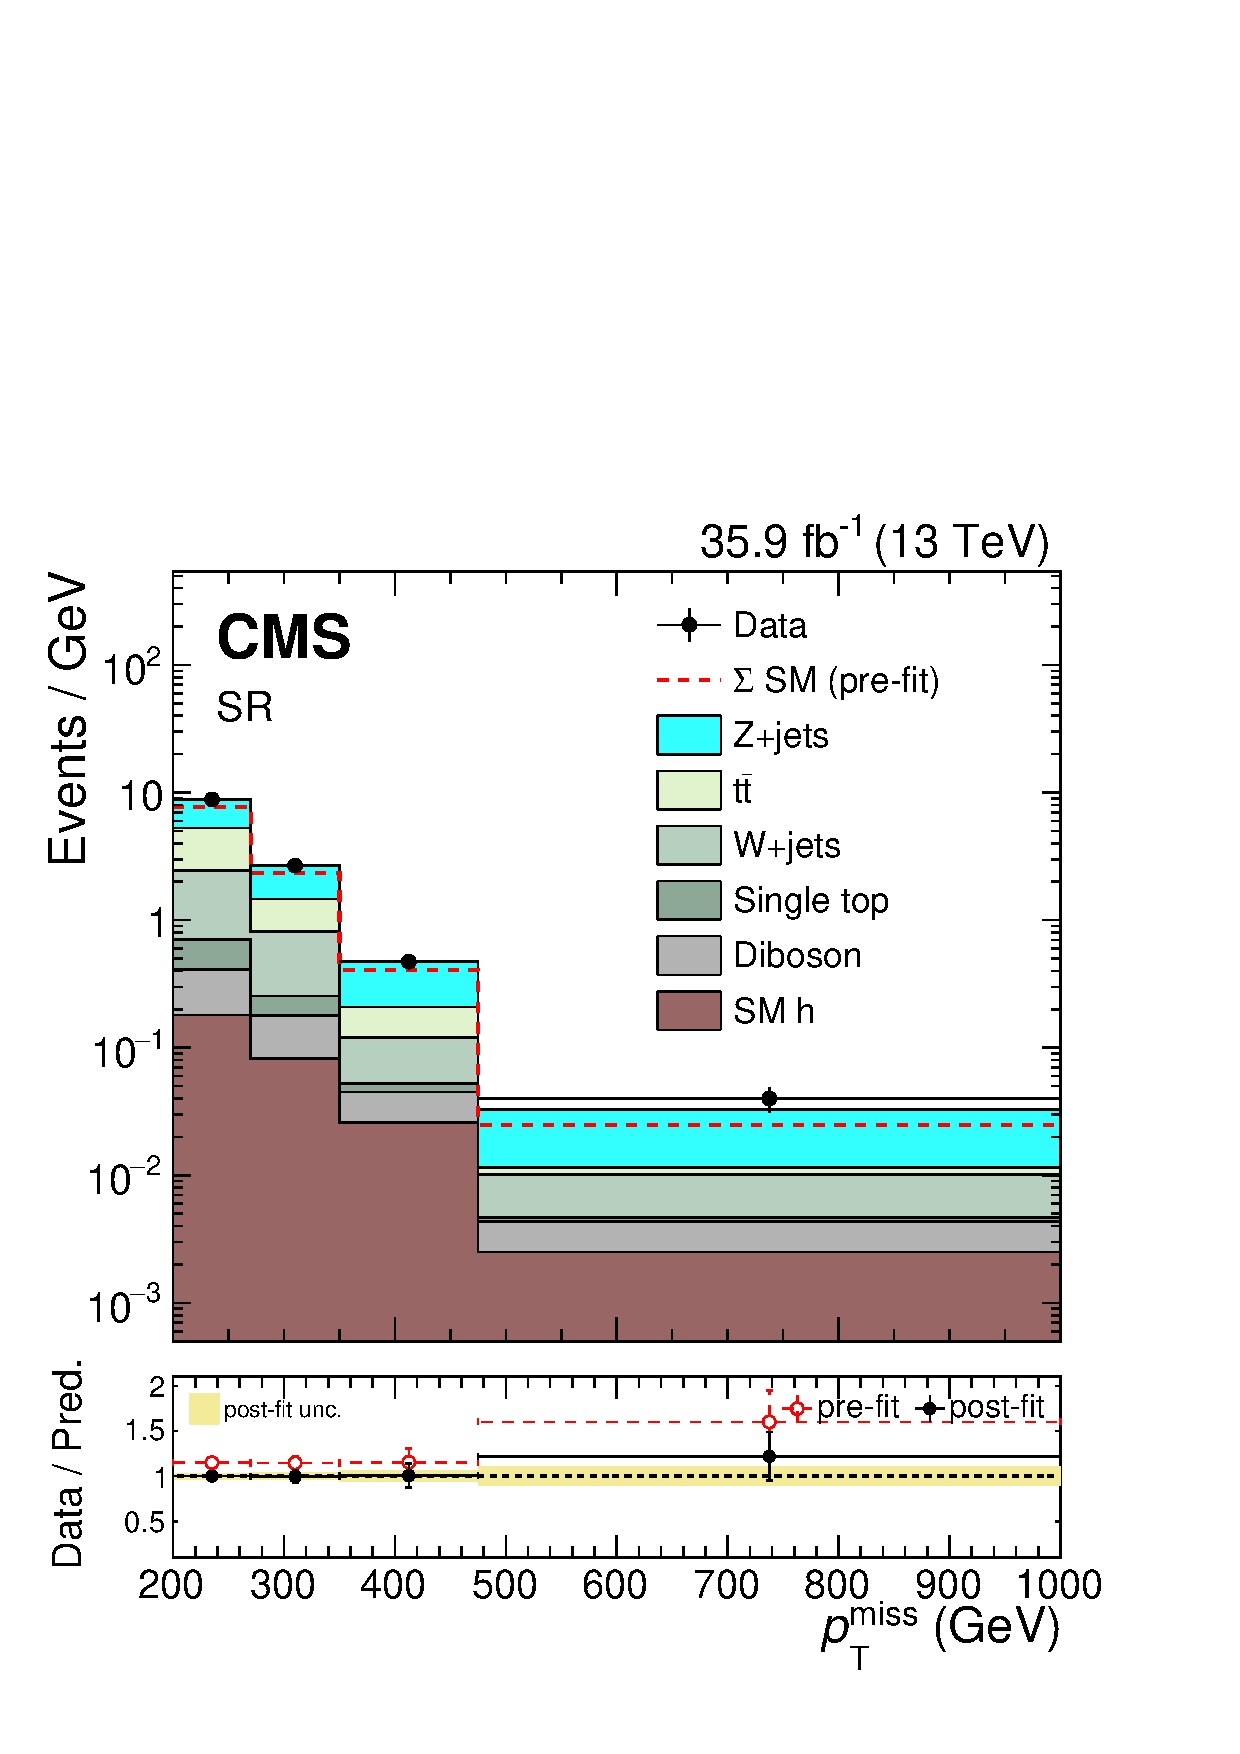
\includegraphics[width=0.45\textwidth]{figures/limits/MSDcorr_stackedPostfit_signal.pdf}}
% \subfloat{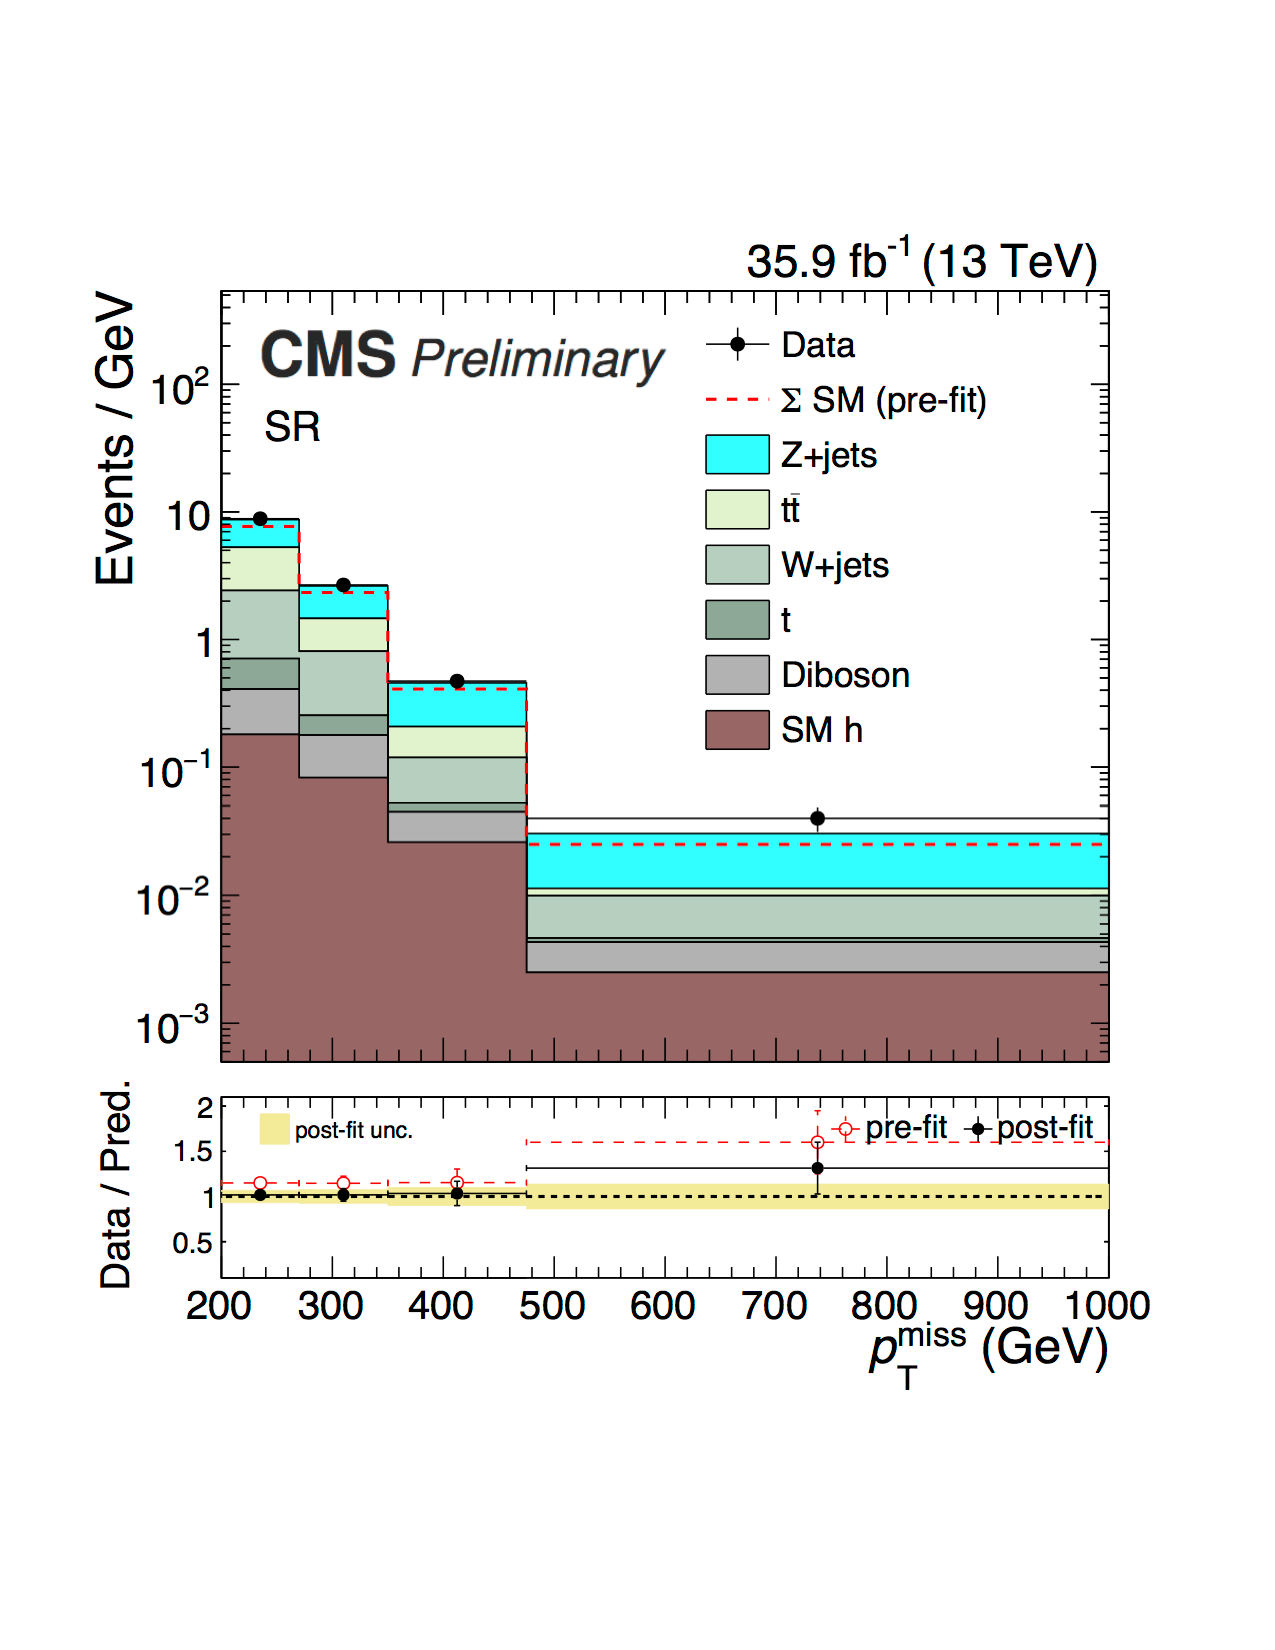
\includegraphics[width=0.45\textwidth]{figures/limits/MSDcorr_stackedPostfit_signal_masked.pdf}} \\
\caption{The \MET distribution in the signal region before and after a likelihood fit. The data are in agreement with post-fit background predictions for the SM backgrounds, and no significant excess is observed. The dashed red histogram corresponds to the pre-fit estimate for the SM backgrounds.}
\label{Fig_sr}
\end{figure}

\begin{table}\footnotesize
\begin{center}
  \caption{Post-fit event yield expectations per \ptmiss bin for the SM backgrounds in the signal region when including the signal region data in the likelihood fit, under the background-only assumption. Quoted are also the expected yields for two signal models. Uncertainties quoted in the predictions include both the systematic and statistical components.}
\\  
\begin{tabular}{l r r r r}
  \hline\hline
\ptmiss-bin         & 200-270\,GeV          & 270-350\,GeV          & 350-475\,GeV          & $>475$\,GeV         \\
\hline
Z+jets          &$ 249\pm22 $       & $97.2\pm8.5$         & $32.6\pm3.6$          & $11.1\pm1.9$       \\
\ttbar          &$ 199\pm14 $       & $52.1\pm5.2$          & $11.1\pm2.0$          & $0.7\pm0.4$        \\
W+jets          &$ 122\pm22 $       & $45.0\pm8.7$          & $8.4\pm1.9$           & $2.9\pm0.9$            \\
Single top quark      &$21.0\pm4.2 $          & $6.1\pm1.2$           & $0.9\pm0.2$           & $0.2\pm0.1$         \\
Diboson         &$ 16.0\pm3.1  $        & $7.6\pm1.5$           & $2.4\pm0.5$           & $1.0\pm0.2$ \\
SM h             &$ 12.6\pm1.4 $      & $ 6.6\pm0.7$           & $ 3.3 \pm 0.3$        & $ 1.3\pm 0.1$      \\
\hline
$\Sigma~(\text{SM})$ & $619\pm20$ & $214.6 \pm 8.1$       & $58.7\pm3.7$          & $17.2 \pm 2.0$ \\

\hline
Data            & $619$       & $ 214$        & $59$          & $ 21$ \\
\hline
2HDM+$a$, $m_\text{A}=1\TeV$, $m_\text{a}=150$\GeV & $5.7 \pm 0.6$ & $9.8 \pm 1.1$ & $18.5 \pm 2.1$ & $5.2 \pm 0.6$\\
Bar. Z', $m_{\text{Z}'}=0.2\TeV$, $m_\chi=50$\GeV & $184 \pm 20$ & $118 \pm 13$ & $69.5 \pm 7.7$ & $28.9 \pm 3.3$\\
\hline\hline
  \end{tabular}
\label{tab:eventYieldTable}
\end{center}
\end{table}

\begin{figure}
\centering
 \subfloat{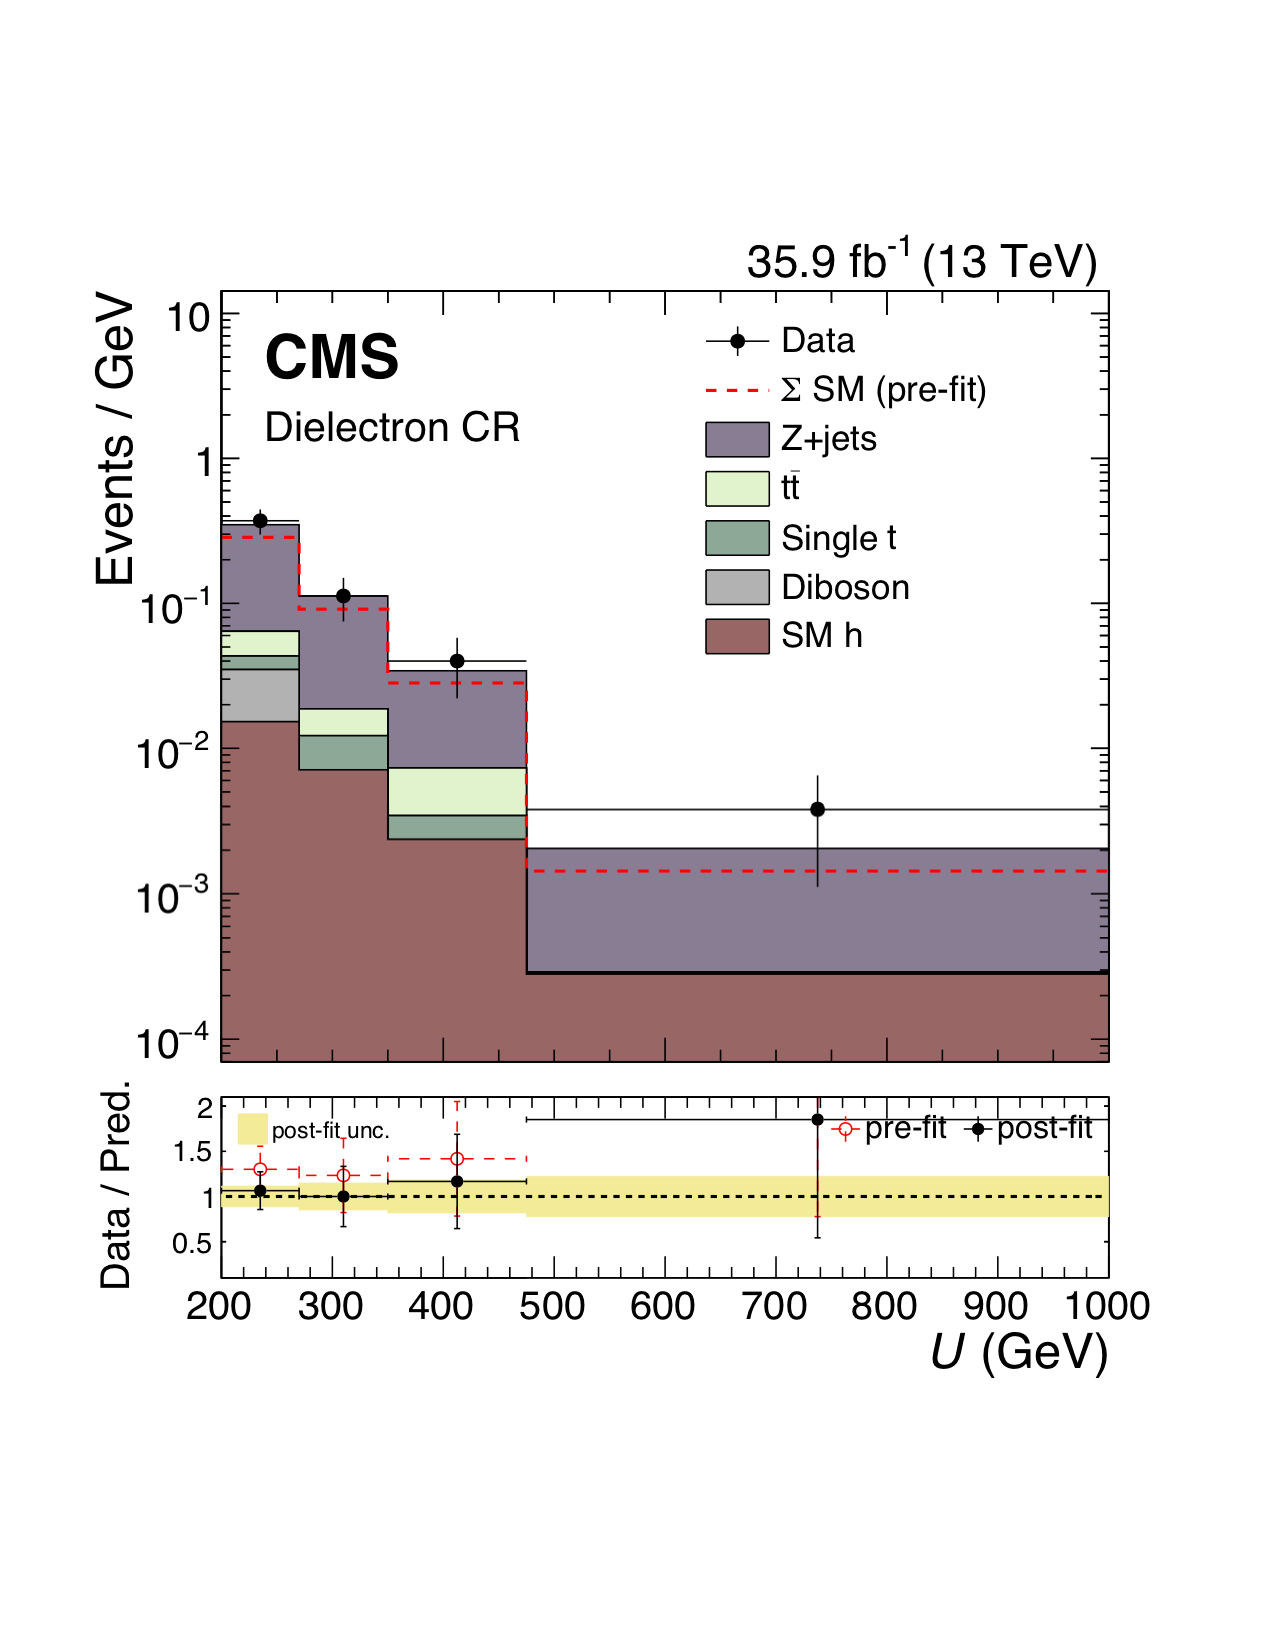
\includegraphics[width=0.36\textwidth]{figures/limits/MSDcorr_stackedPostfit_dielectron.pdf}}
 \subfloat{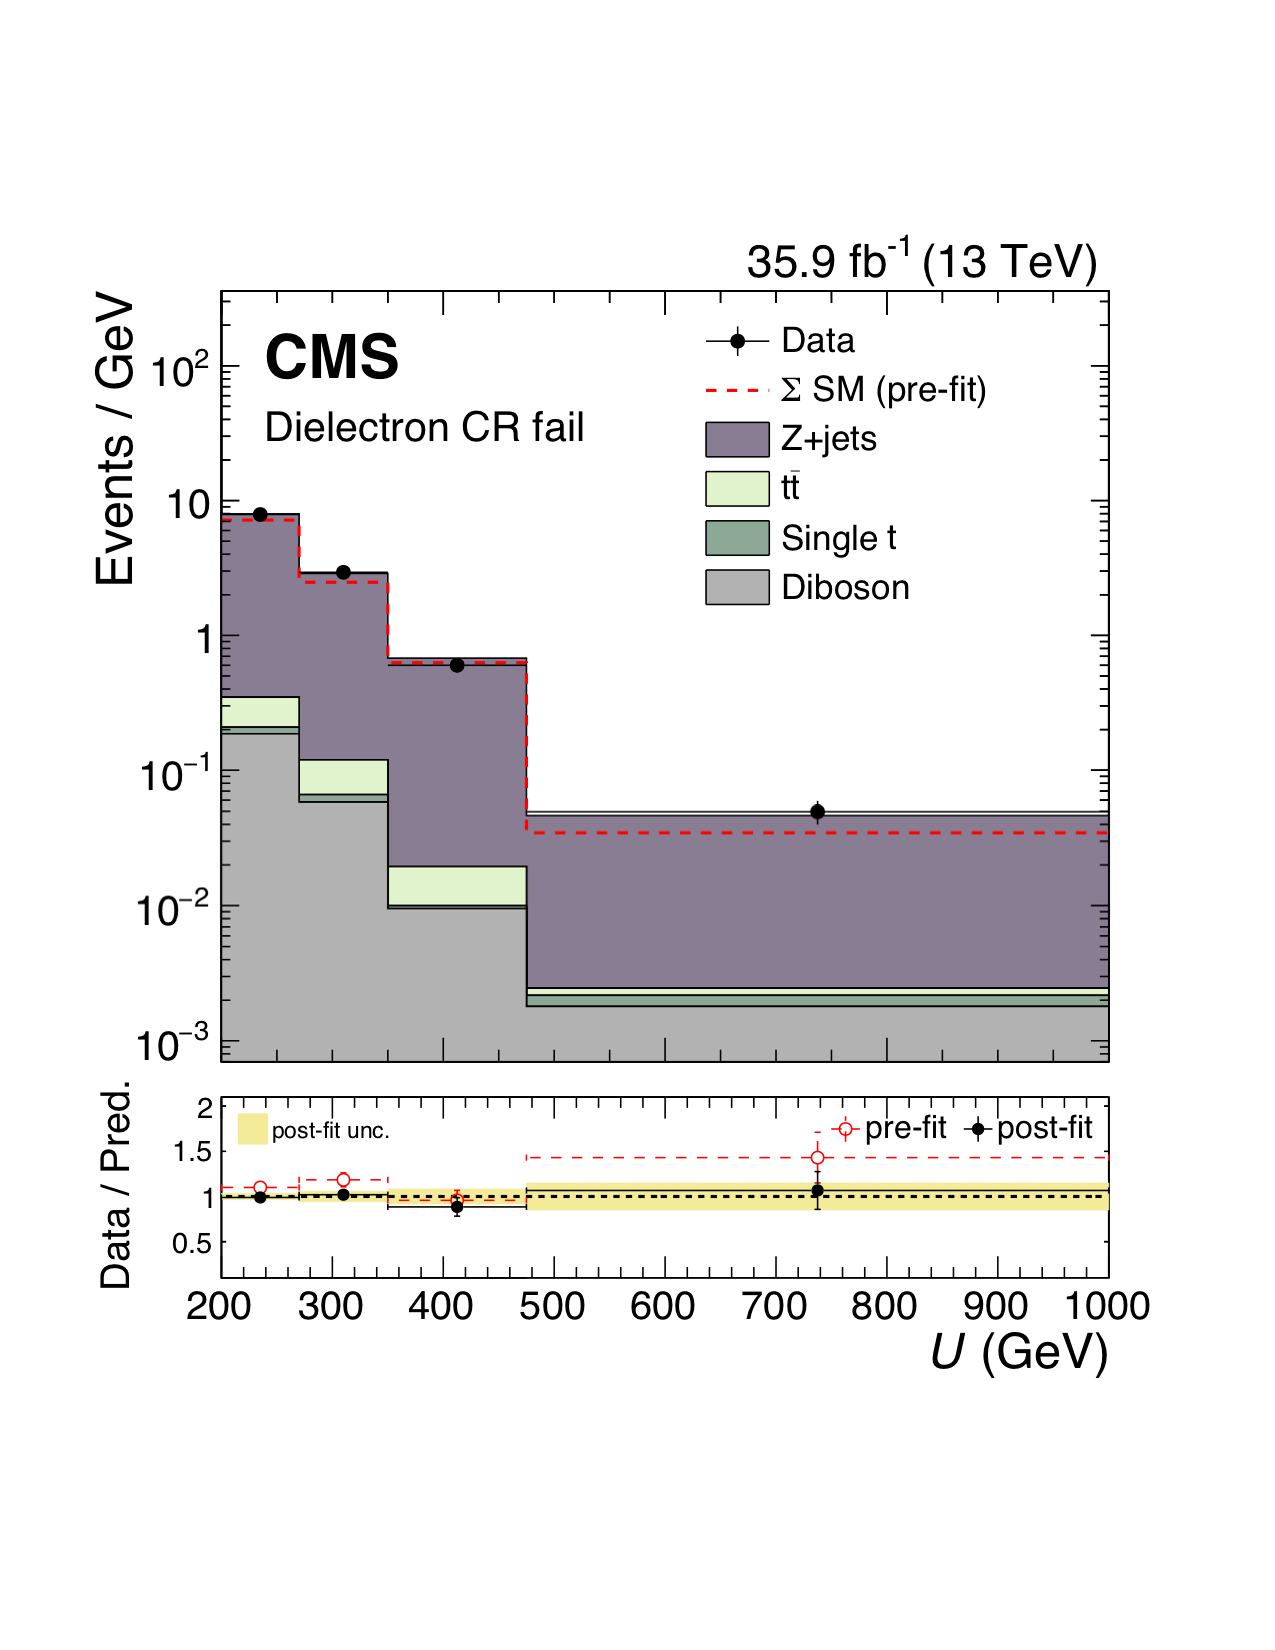
\includegraphics[width=0.36\textwidth]{figures/limits/MSDcorr_stackedPostfit_dielectron_fail.pdf}} \\
 \subfloat{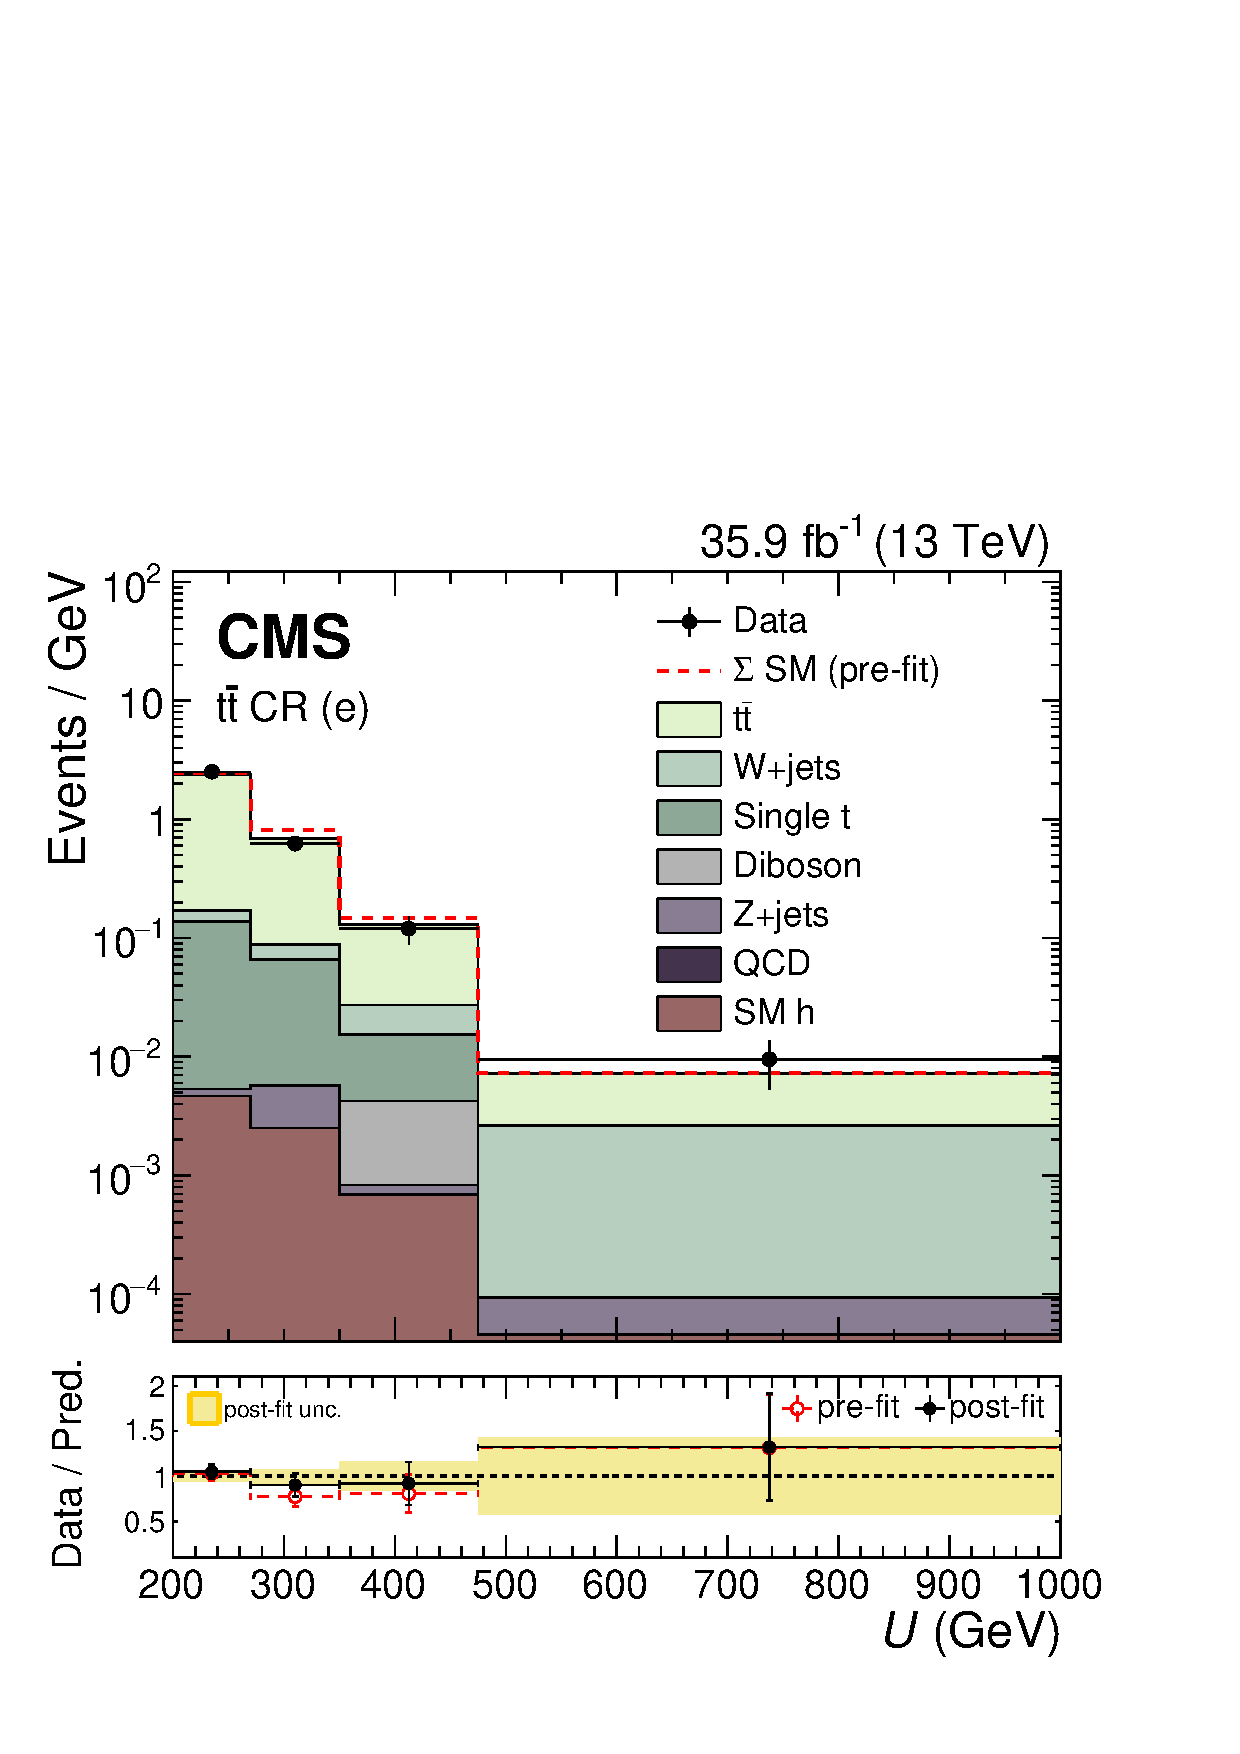
\includegraphics[width=0.36\textwidth]{figures/limits/MSDcorr_stackedPostfit_singleelectrontop.pdf}}
 \subfloat{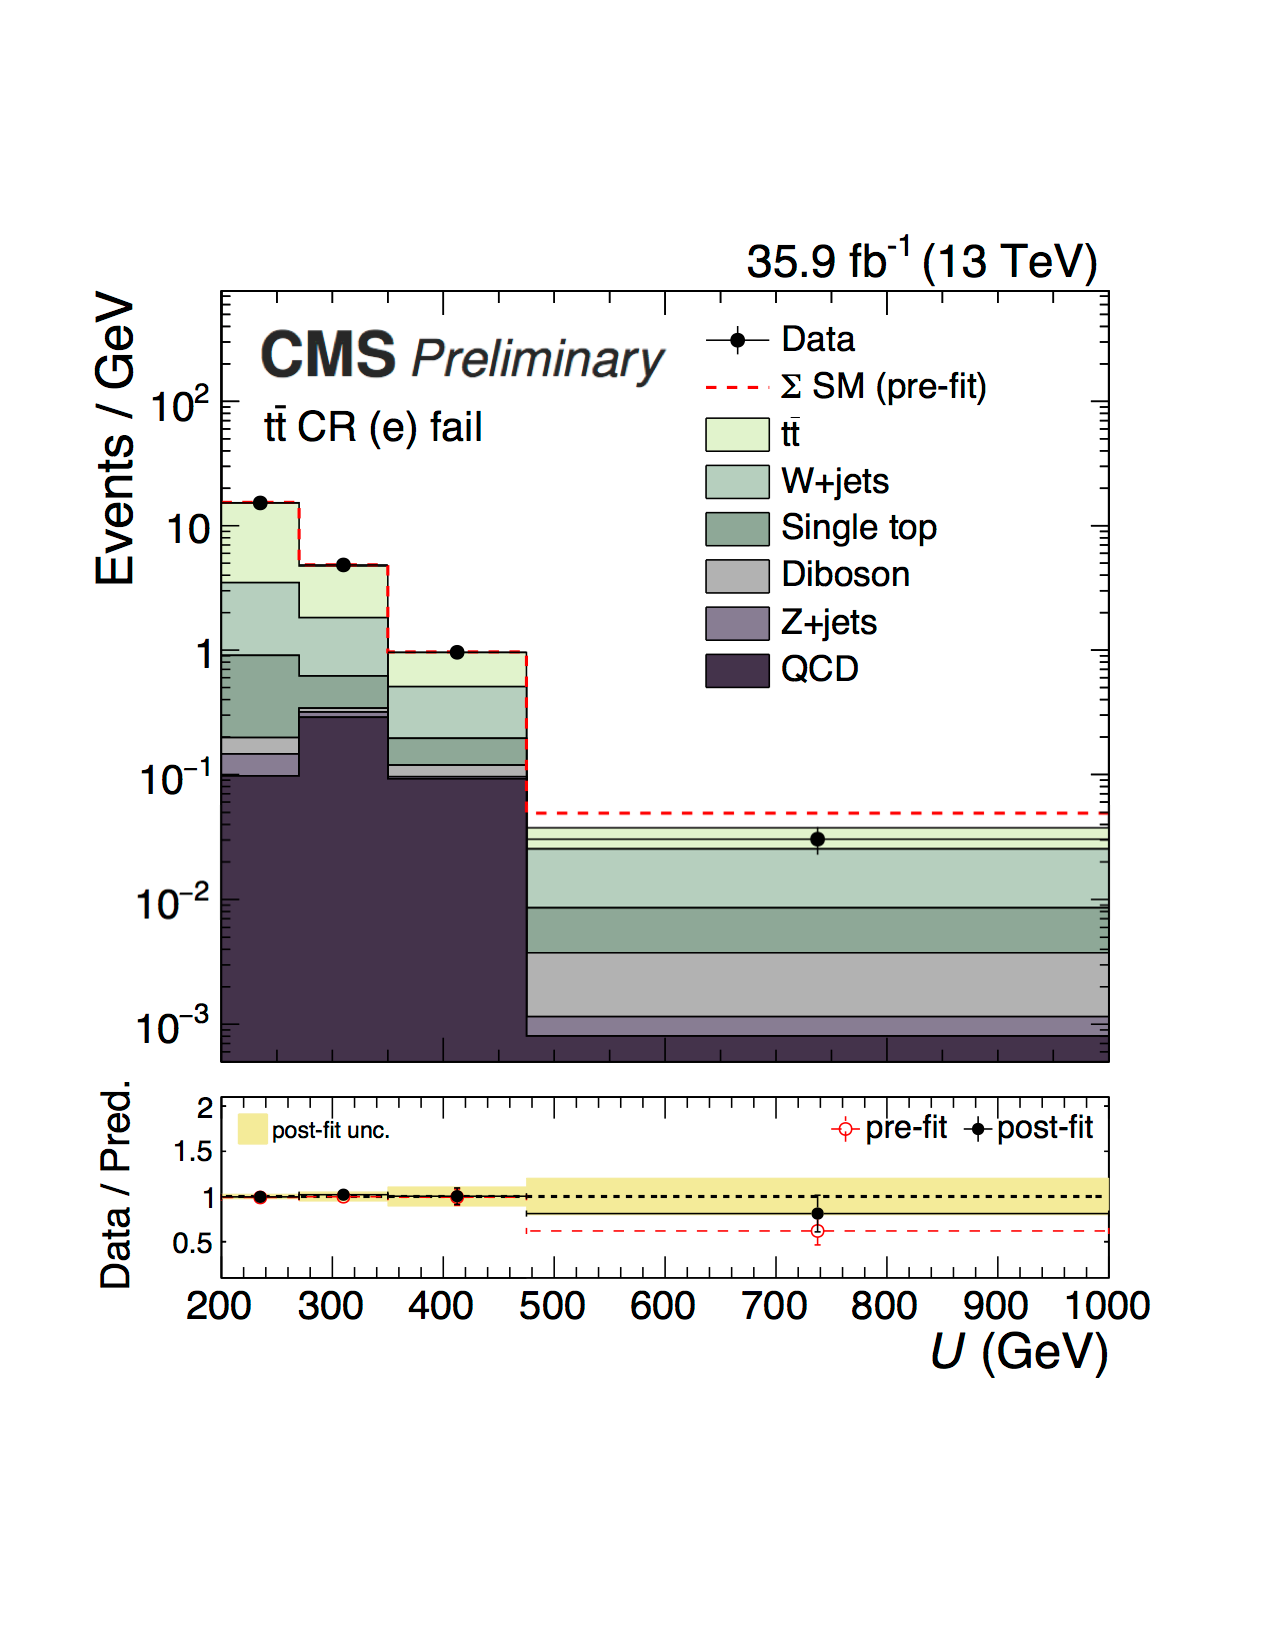
\includegraphics[width=0.36\textwidth]{figures/limits/MSDcorr_stackedPostfit_singleelectrontop_fail.pdf}} \\
 \subfloat{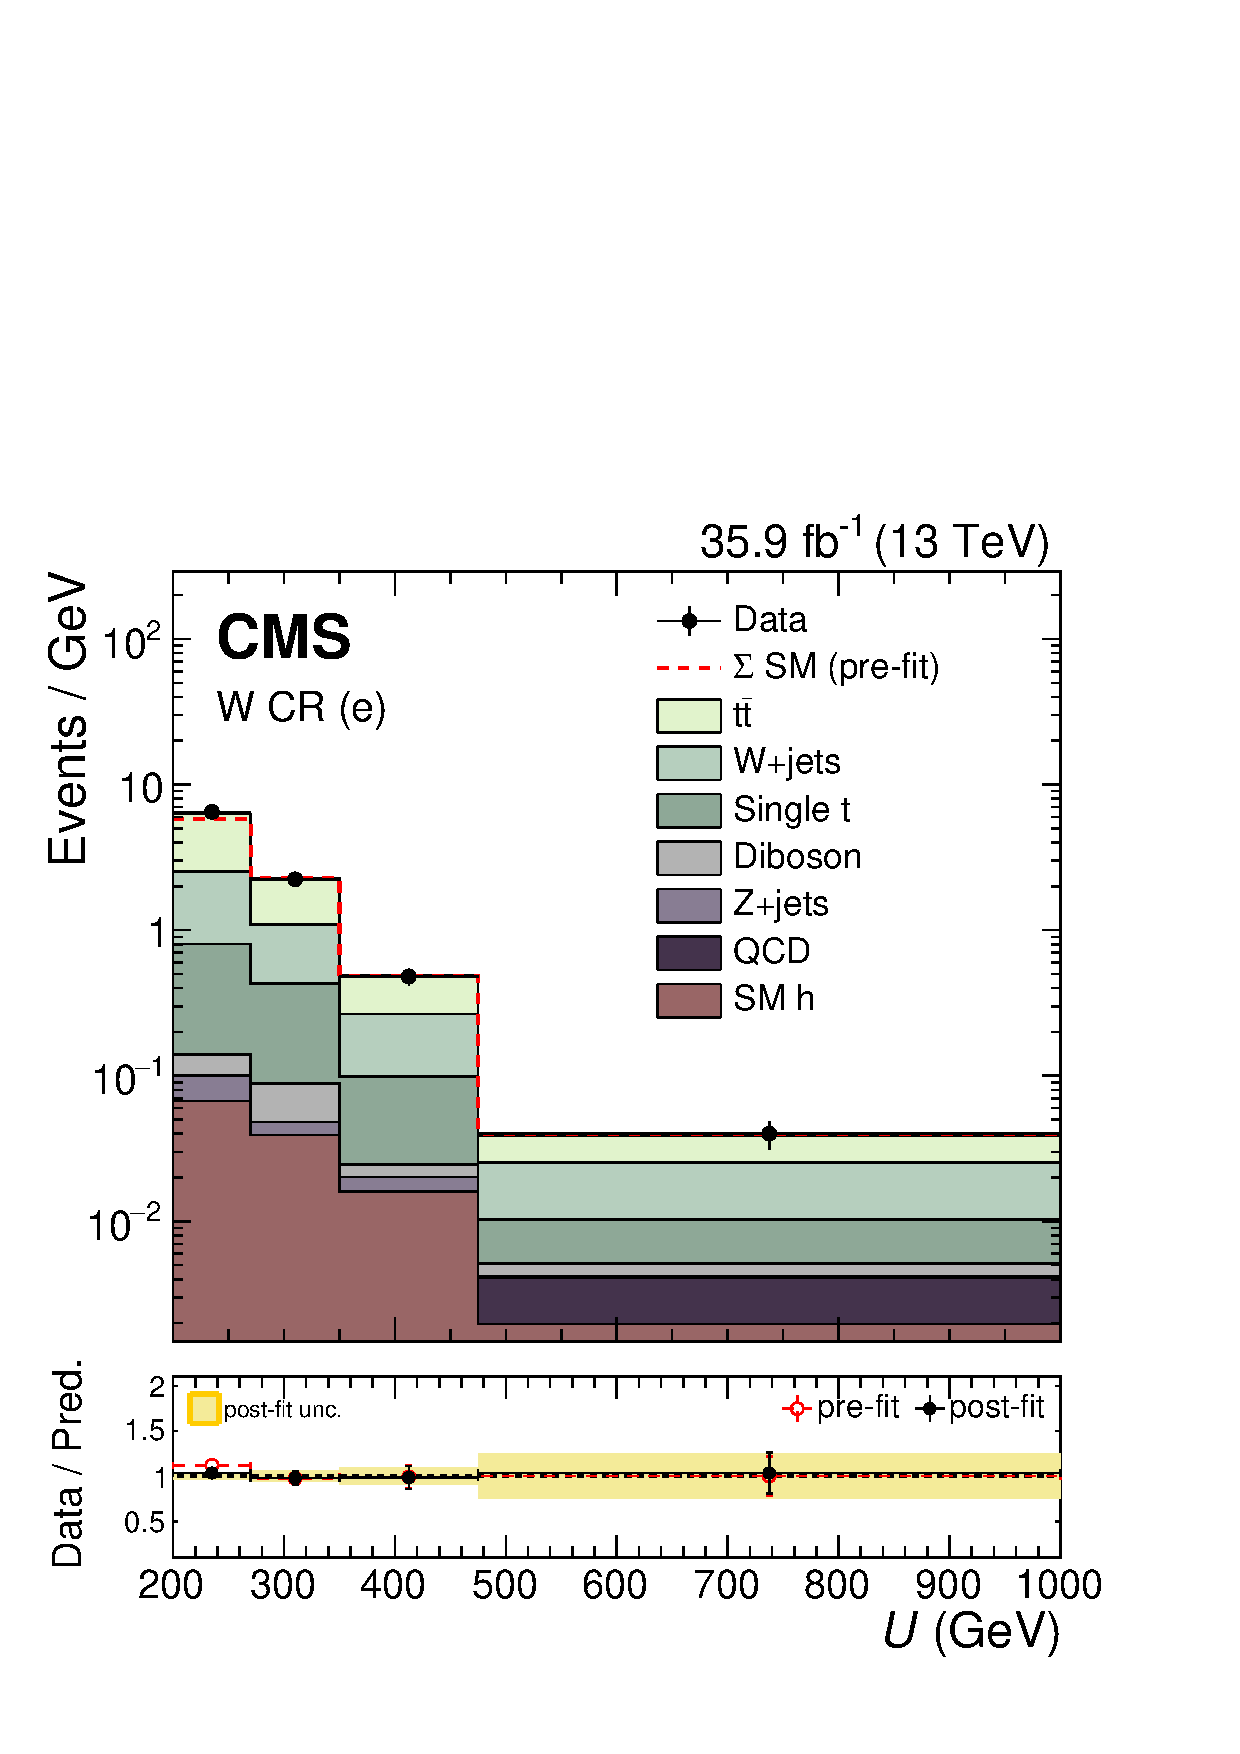
\includegraphics[width=0.36\textwidth]{figures/limits/MSDcorr_stackedPostfit_singleelectronw.pdf}}
 \subfloat{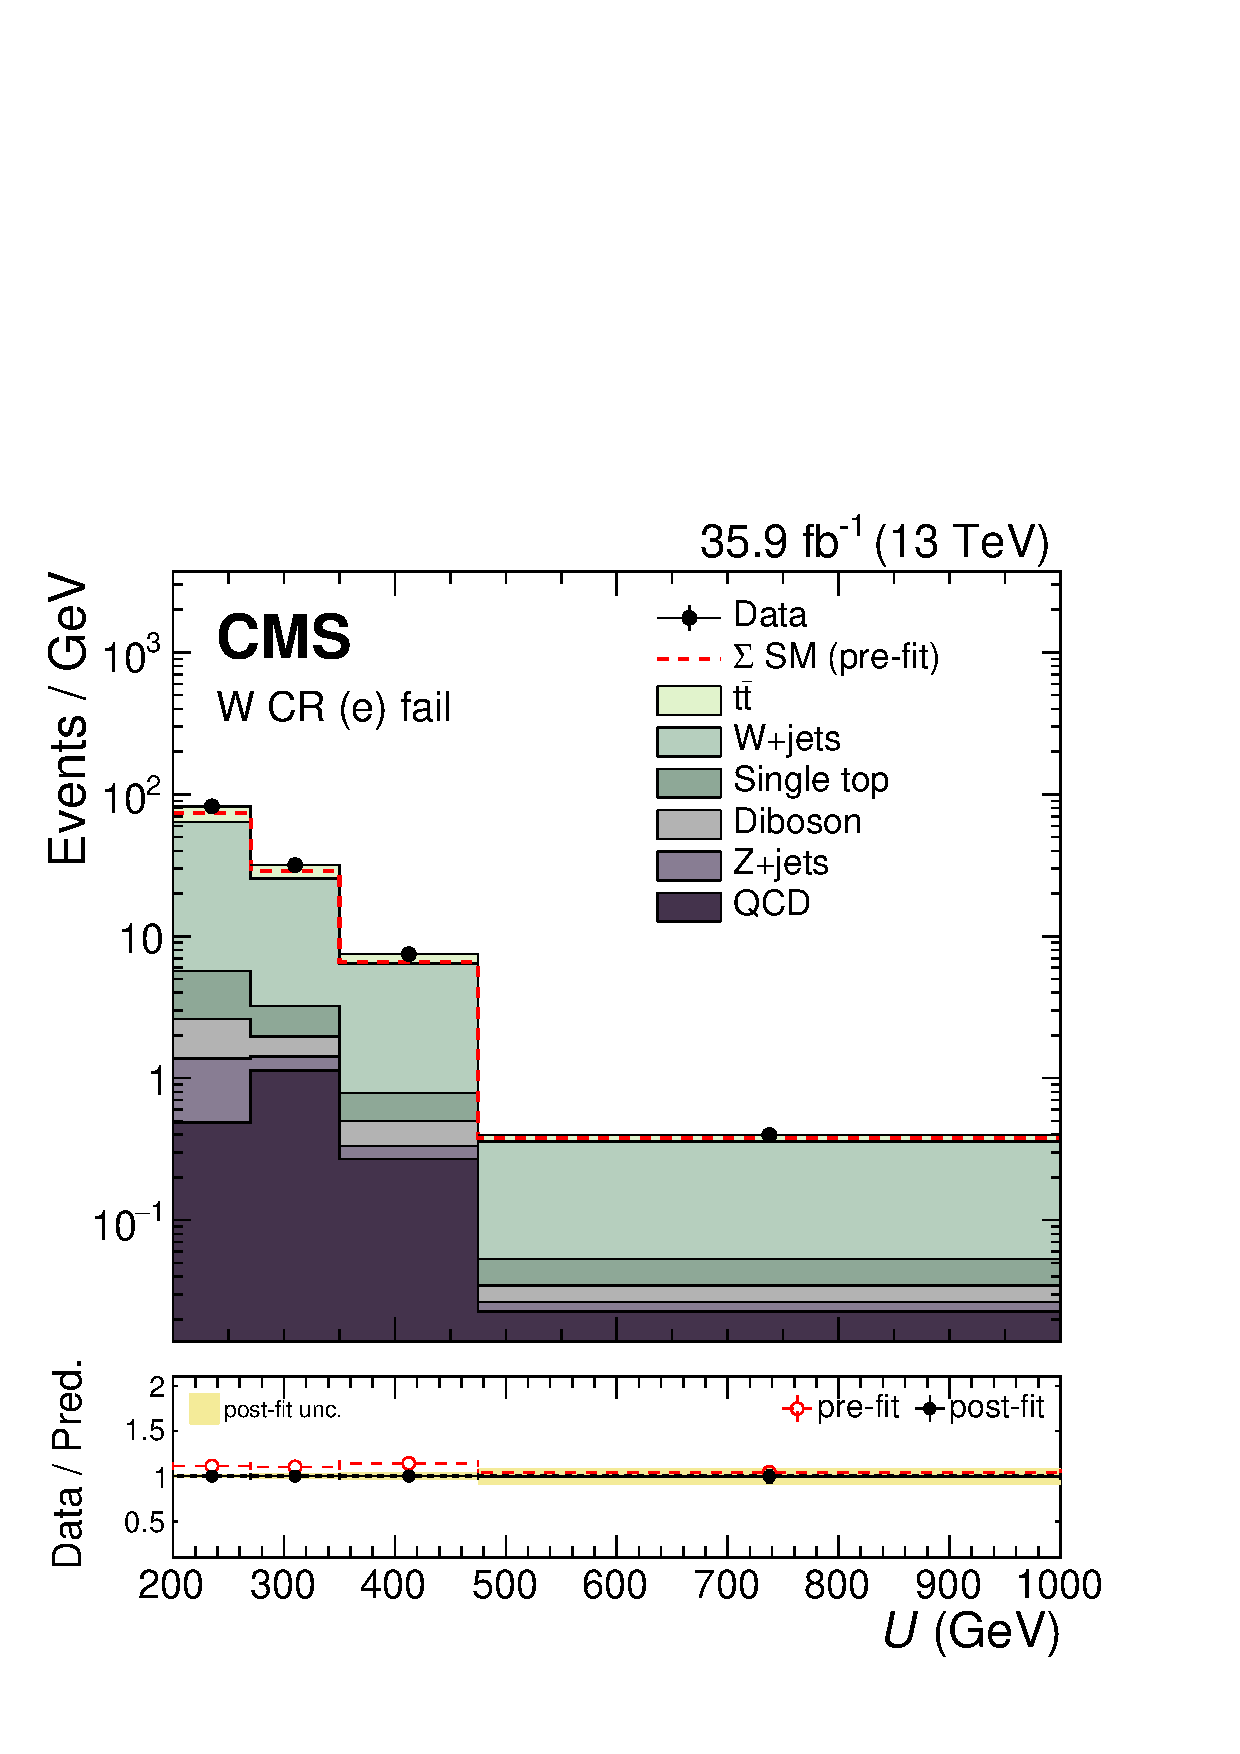
\includegraphics[width=0.36\textwidth]{figures/limits/MSDcorr_stackedPostfit_singleelectronw_fail.pdf}} \\
\caption{The $U$ distribution in the electron control regions before and after a background-only fit to data, including the data in the signal region in the likelihood. For the distributions on the left the CA15 jet passes the double-b tag requirement and for the distributions on the right it fails the double-b tag requirement.}
\label{Fig_cr_2}
\end{figure}


\begin{figure}
\centering
 \subfloat{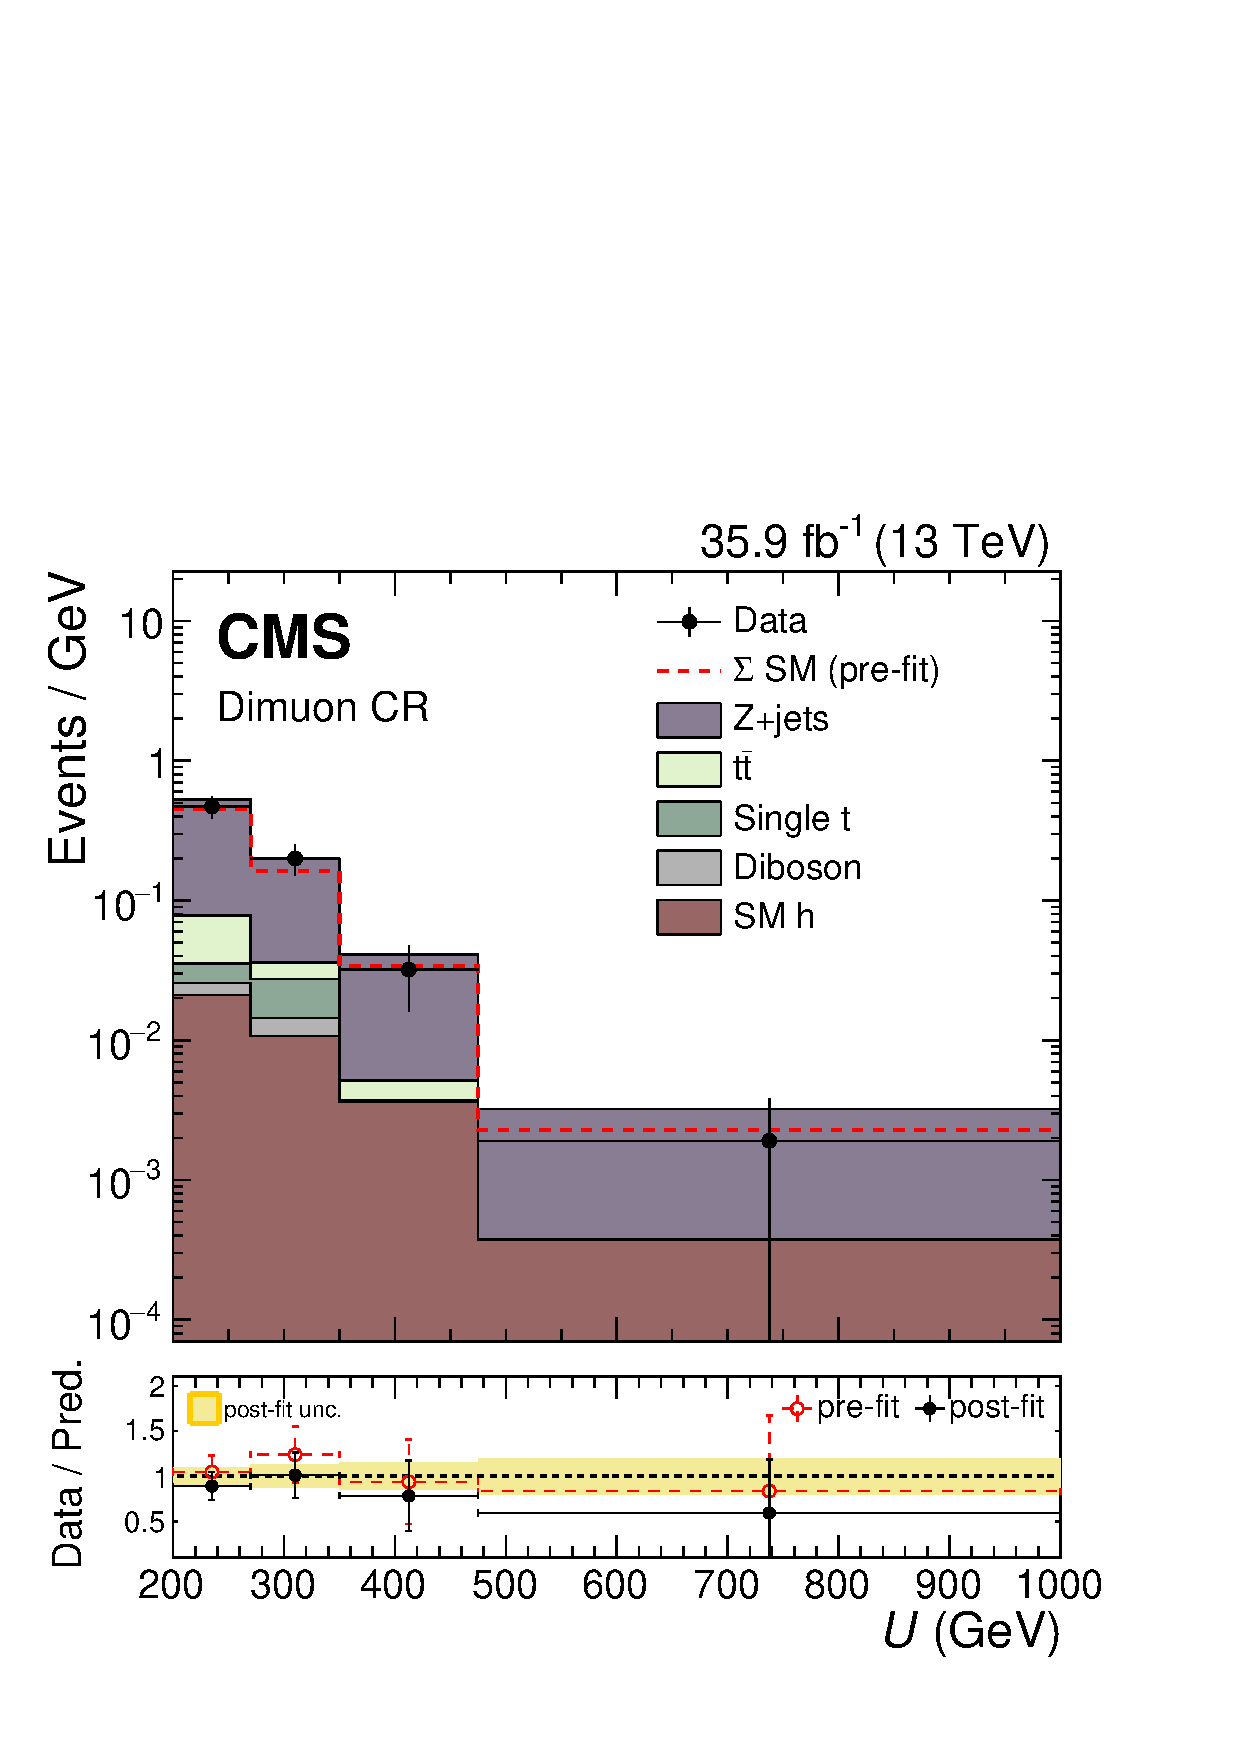
\includegraphics[width=0.36\textwidth]{figures/limits/MSDcorr_stackedPostfit_dimuon.pdf}}
 \subfloat{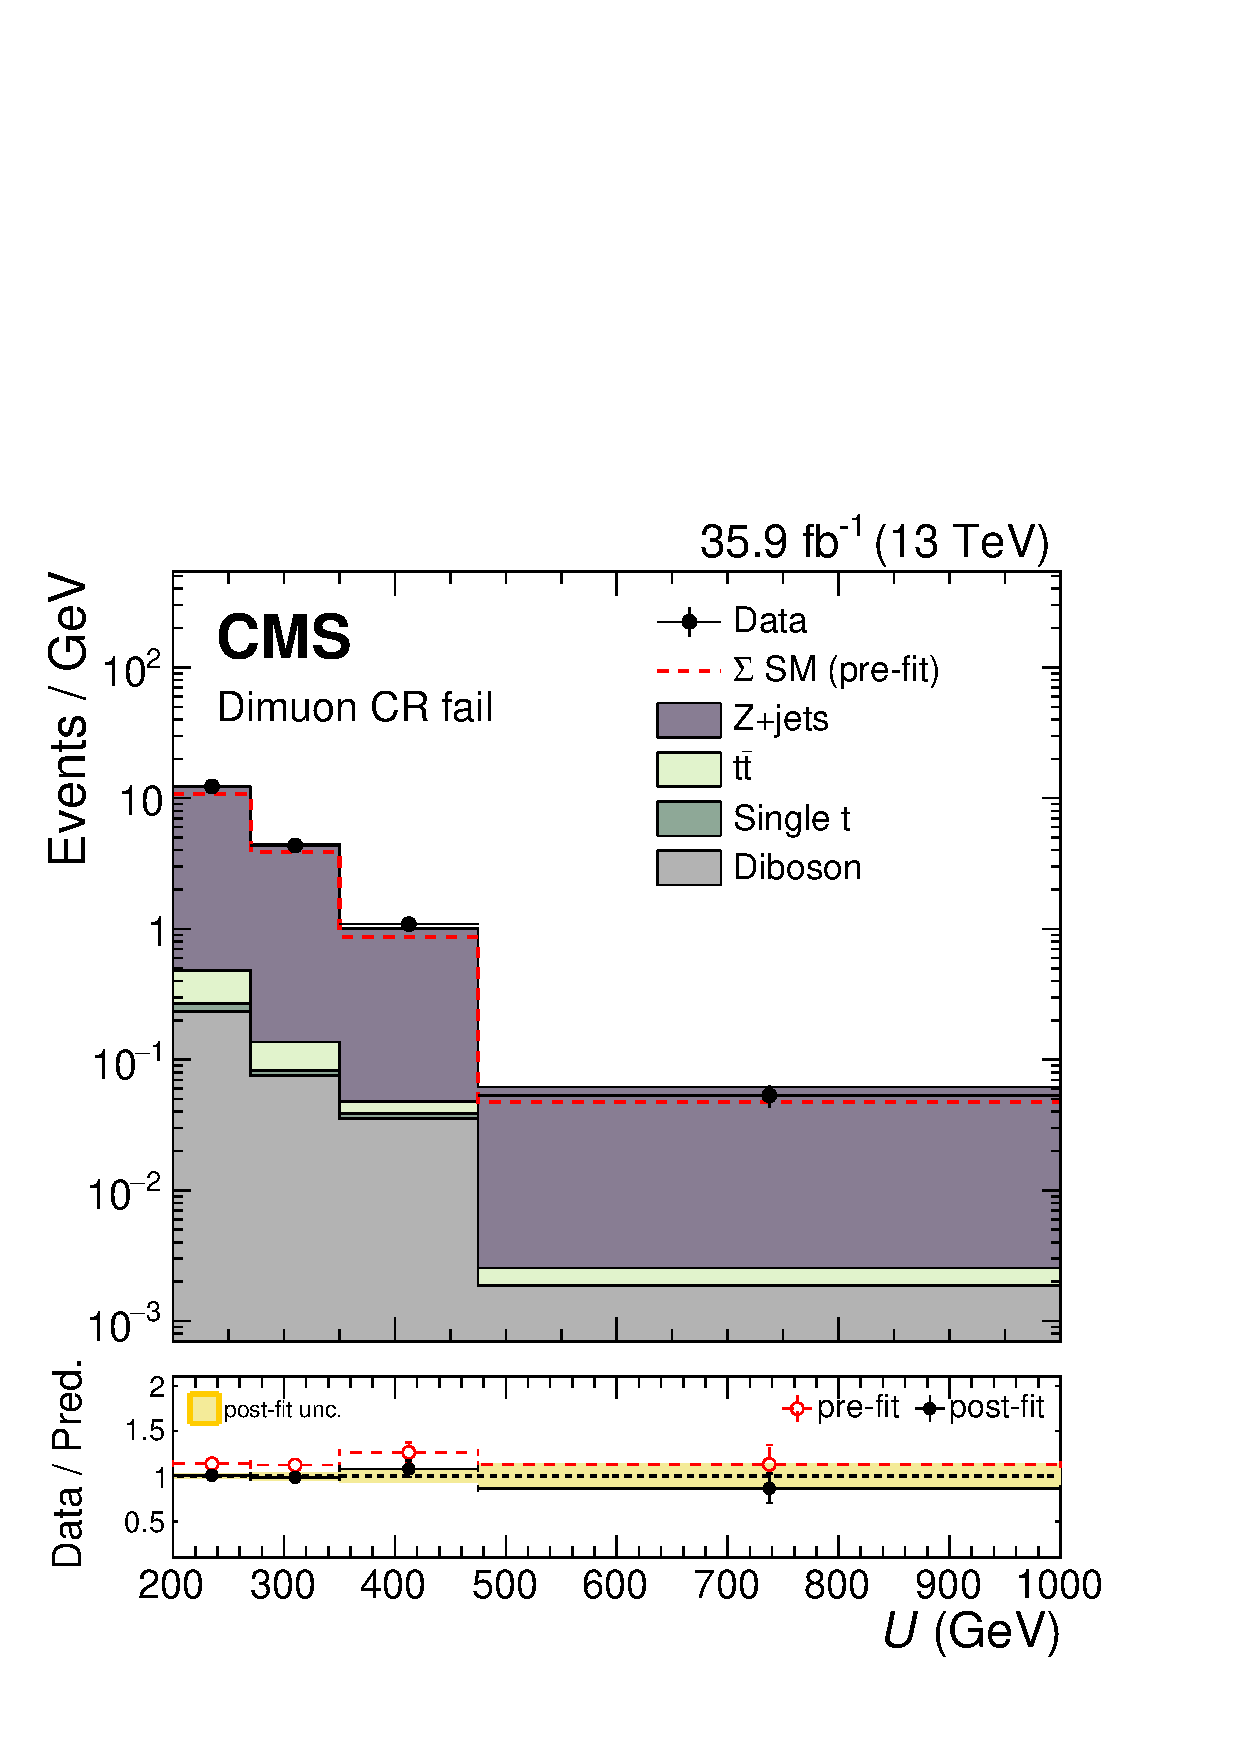
\includegraphics[width=0.36\textwidth]{figures/limits/MSDcorr_stackedPostfit_dimuon_fail.pdf}} \\
 \subfloat{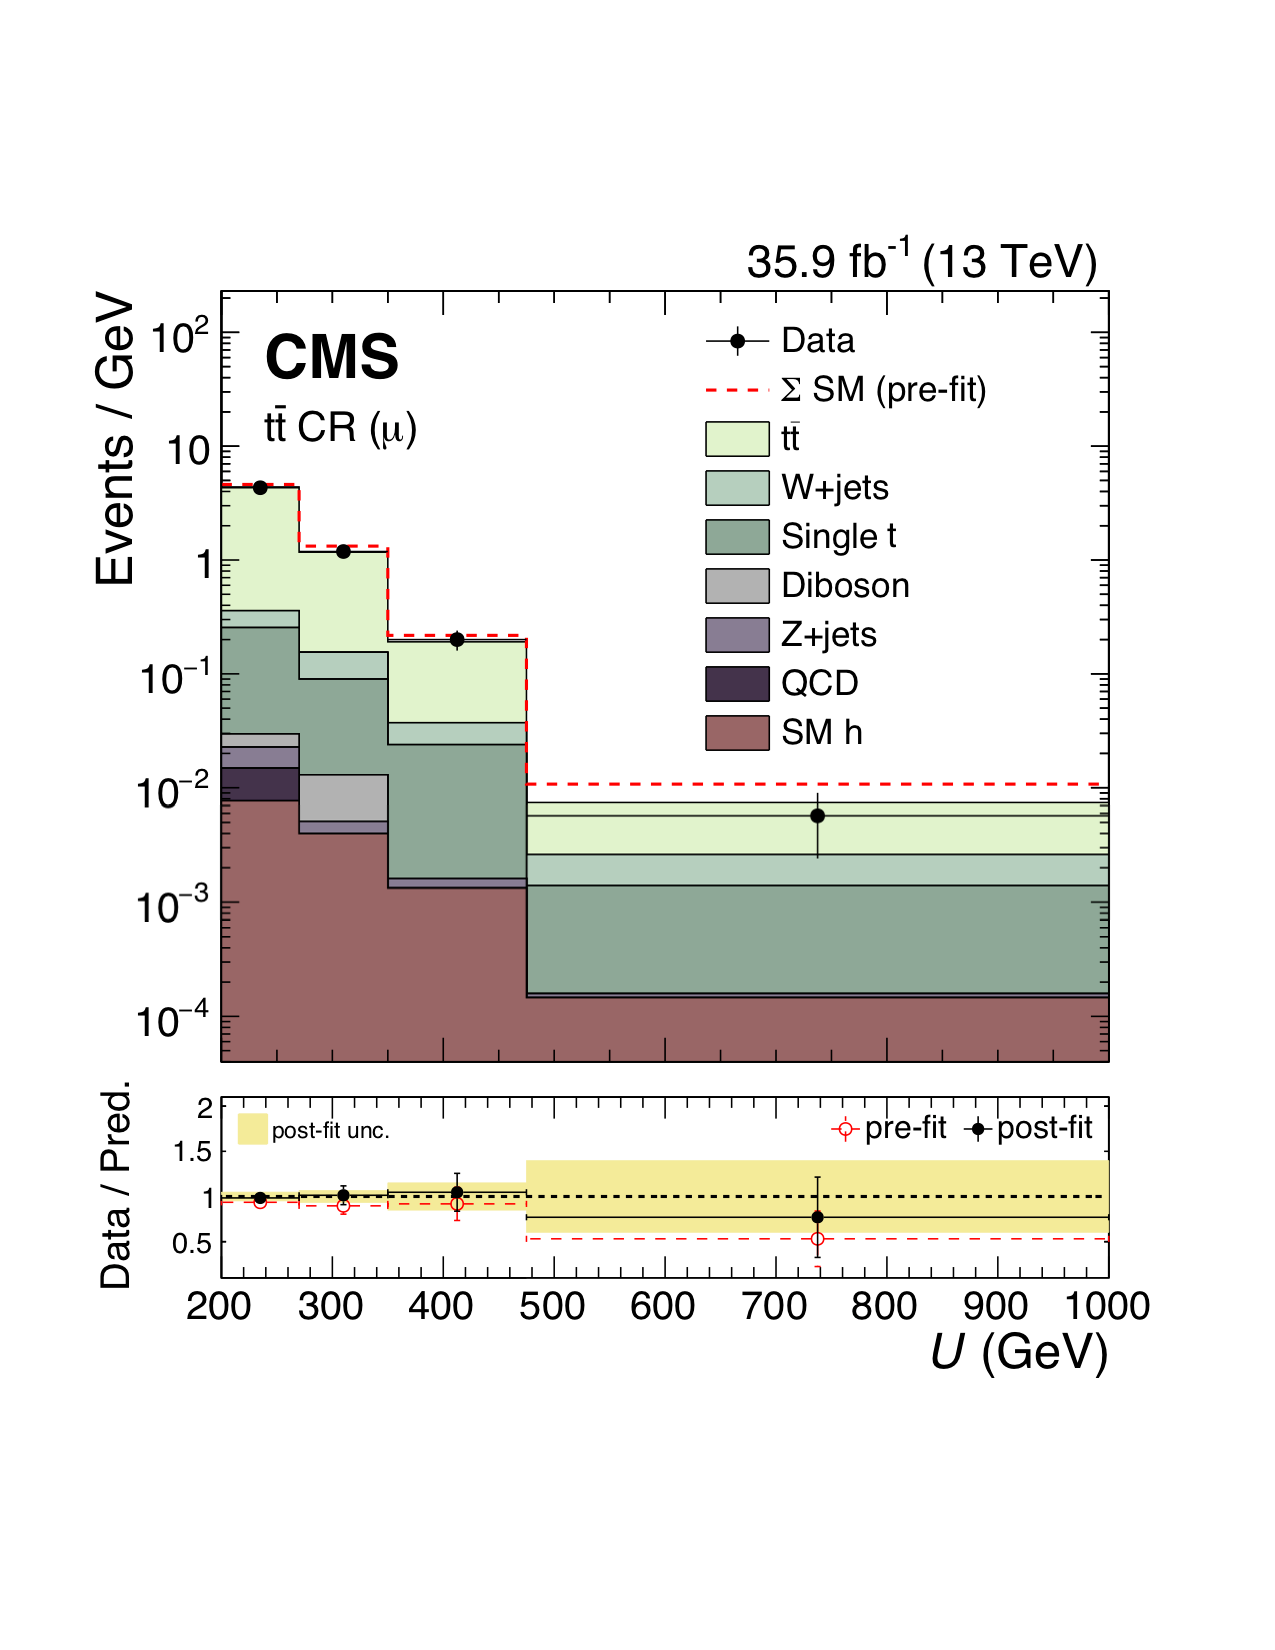
\includegraphics[width=0.36\textwidth]{figures/limits/MSDcorr_stackedPostfit_singlemuontop.pdf}}
 \subfloat{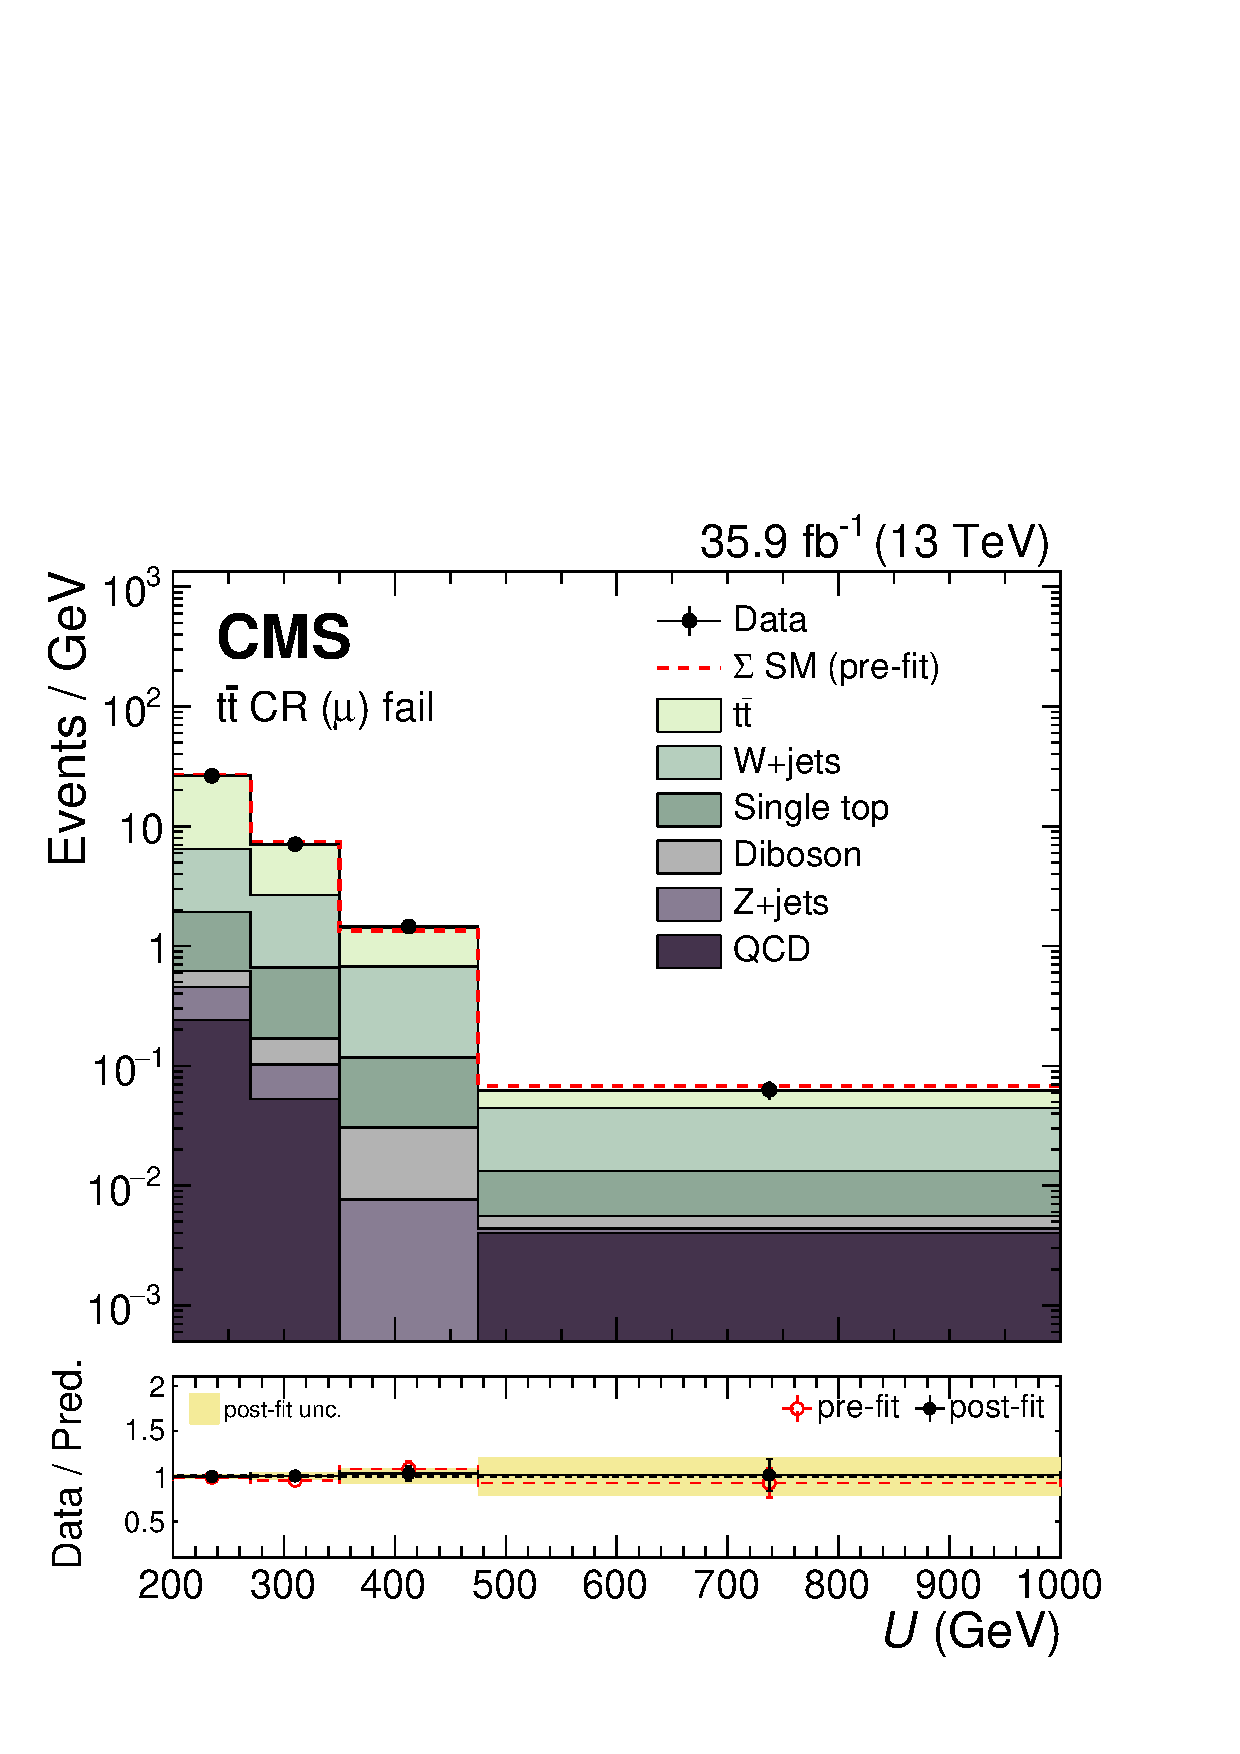
\includegraphics[width=0.36\textwidth]{figures/limits/MSDcorr_stackedPostfit_singlemuontop_fail.pdf}} \\
 \subfloat{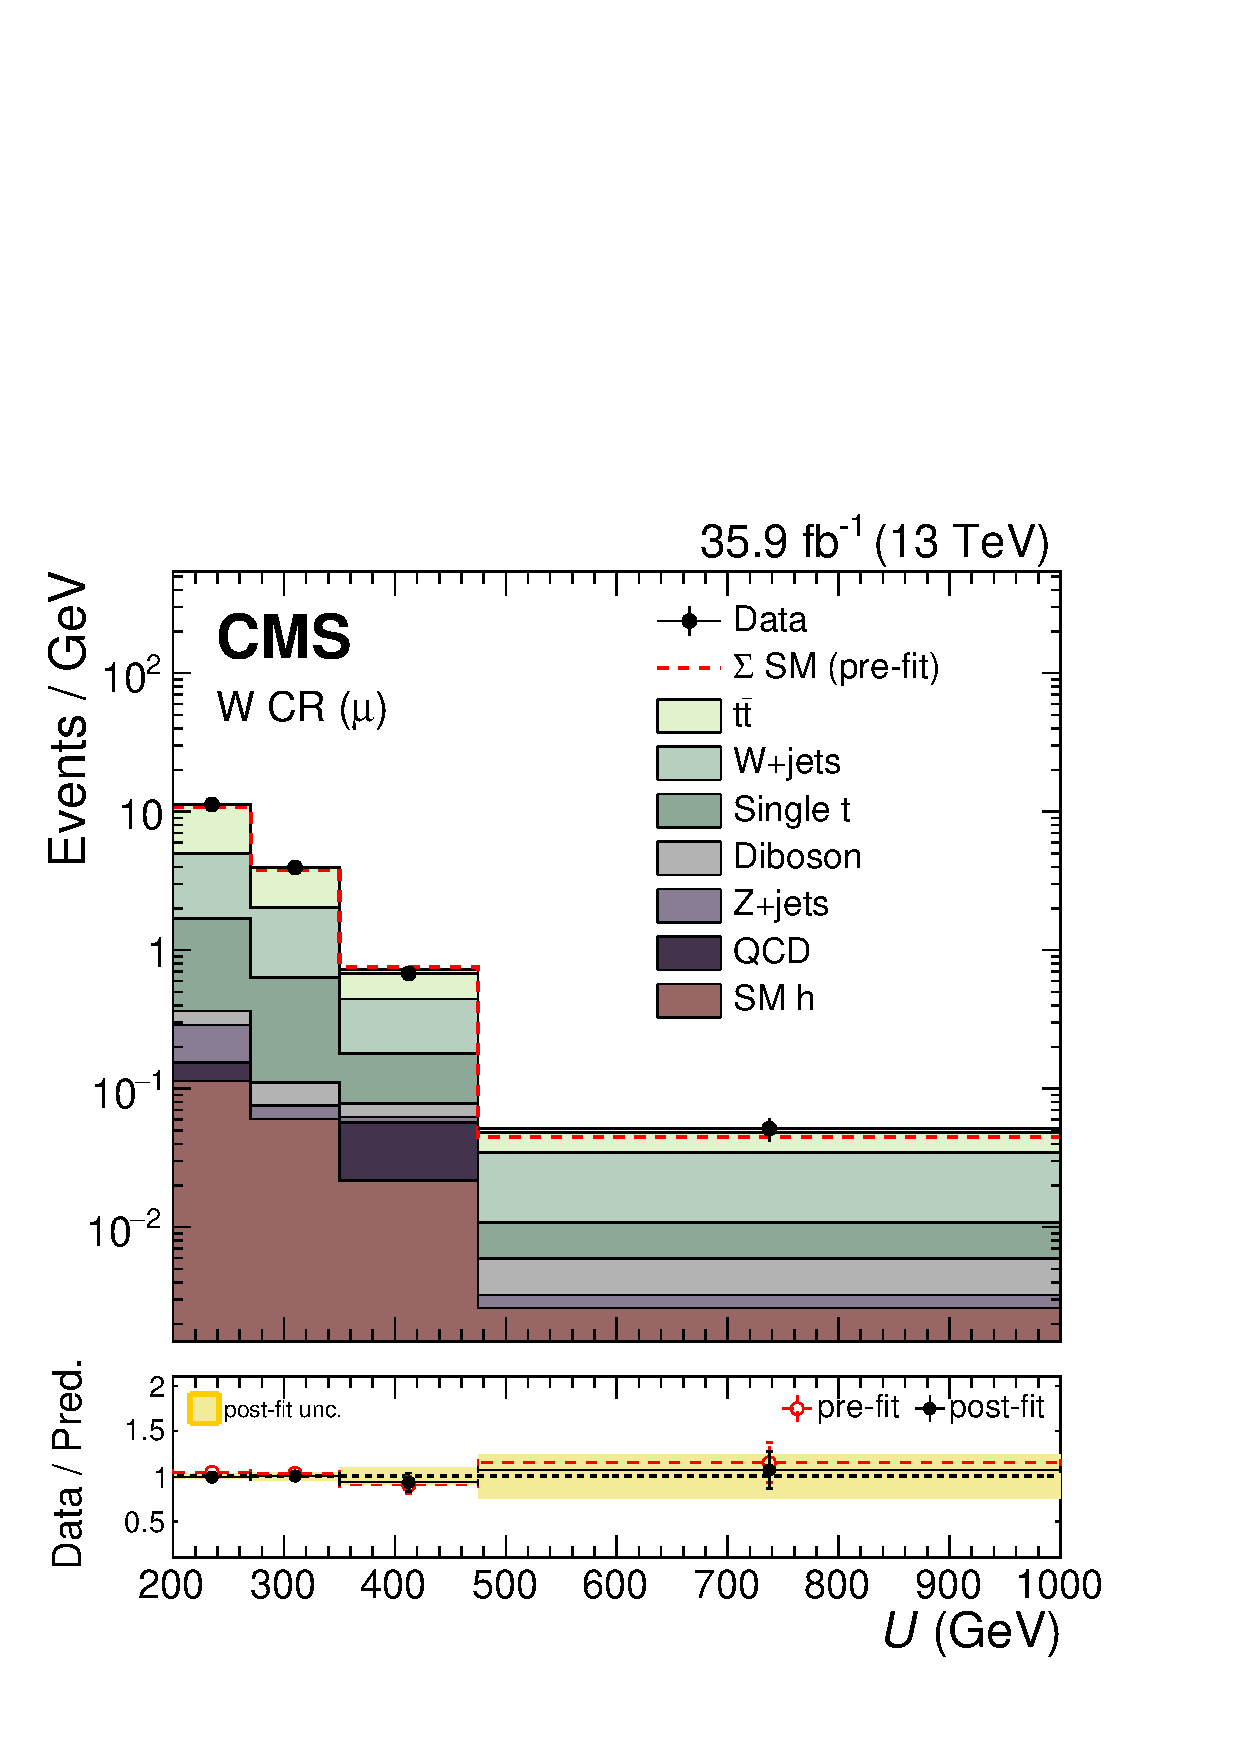
\includegraphics[width=0.36\textwidth]{figures/limits/MSDcorr_stackedPostfit_singlemuonw.pdf}}
 \subfloat{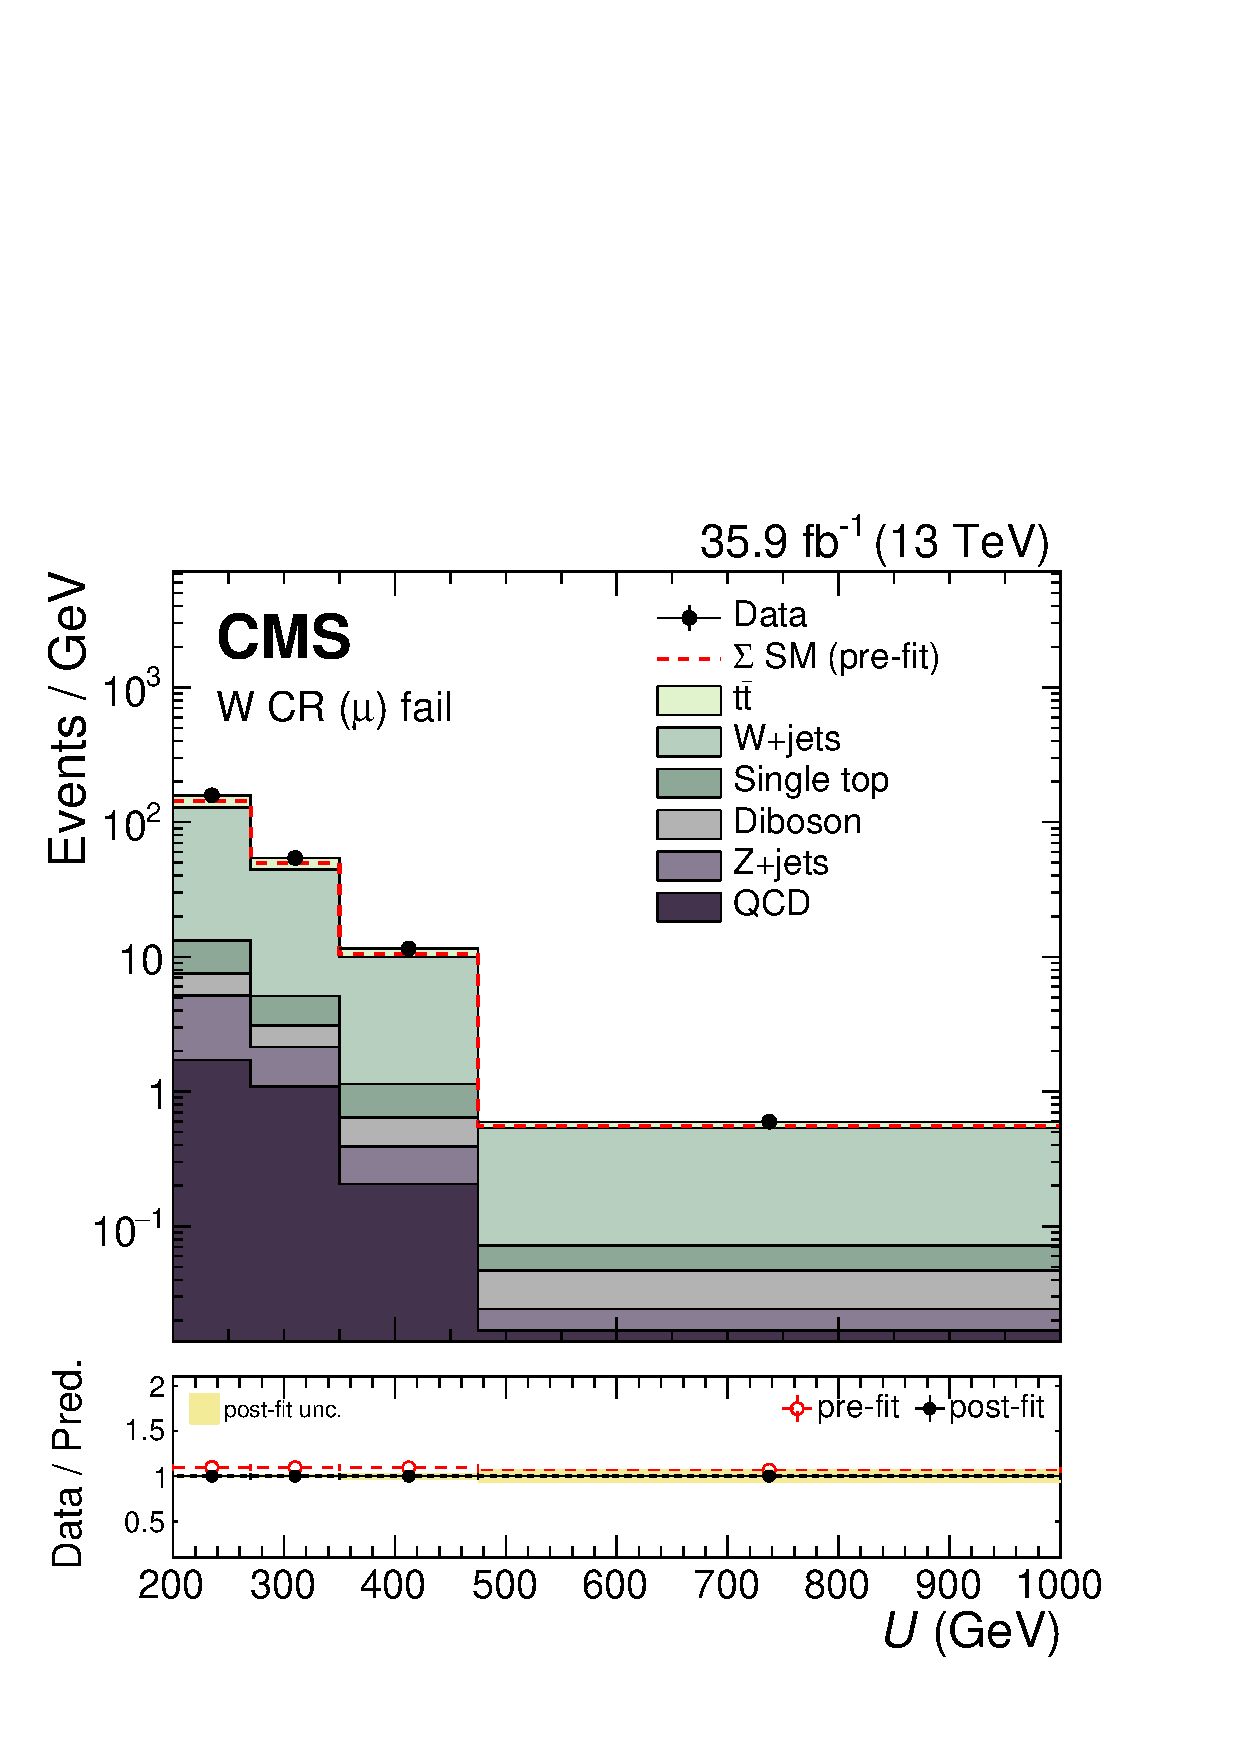
\includegraphics[width=0.36\textwidth]{figures/limits/MSDcorr_stackedPostfit_singlemuonw_fail.pdf}} \\
 \caption{The $U$ distribution in the muon control regions before and after a background-only fit to data, including the data in the signal region in the likelihood. For the distributions on the left the CA15 jet passes the double-b tag requirement and for the distributions on the right it fails the double-b tag requirement.}
\label{Fig_cr_1}
\end{figure}

No significant excess over the SM background expectation is observed in the SR. The results of this search are interpreted in terms of upper limits on the signal strength modifier $\mu=\sigma/\sigma_\text{theory}$, where $\sigma_\text{theory}$ is the predicted production cross 
section of DM candidates in association with a Higgs boson and $\sigma$ is the upper limit on the observed cross section. 
The upper limits are calculated at 95\% confidence level (CL) using a modified frequentist method (CL$_s$) \cite{yellowReport, bib:CLS1, bib:CLS2} computed with an asymptotic approximation \cite{bib:CLS3}. 


%\begin{table}\footnotesize
%\begin{center}
%  \caption{Per-\ptmiss-bin post-fit event yield expectations for the SM backgrounds in the signal region when masking the signal region data from the likelihood fit. Uncertainties quoted on the predictions include systematic and statistical uncertainties.}
%\begin{tabular}{l r r r r}
%  \hline\hline
%\ptmiss-bin         & 200-270\,GeV          & 270-350\,GeV          & 350-475\,GeV          & $>475$\,GeV         \\
%\hline
%Z+jets          &$ 239.2\pm37.9 $       & $93.3\pm14.4$         & $31.1\pm5.5$          & $10.0\pm2.2$       \\
%\ttbar          &$ 200.0\pm13.3 $       & $52.3\pm5.1$          & $11.1\pm2.0$          & $0.7\pm0.4$        \\
%W+jets          &$ 119.8\pm22.4 $       & $44.3\pm8.9$          & $8.3\pm1.9$           & $2.8\pm0.9$            \\
%Single top      &$21.0\pm4.3 $          & $6.1\pm1.3$           & $0.9\pm0.2$           & $0.2\pm0.1$         \\
%Diboson         &$ 16.0\pm3.1  $        & $7.6\pm1.5$           & $2.4\pm0.5$           & $1.0\pm0.2$ \\
%SM h             &$ 12.6\pm1.4 $      & $ 6.6\pm0.7$           & $ 3.3 \pm 0.3$        & $ 1.3\pm 0.1$      \\
%\hline
%$\Sigma~(\text{SM})$ & $608.3\pm41.8$ & $210.2 \pm 15.9$       & $57.1\pm5.7$          & $16.0 \pm 2.2$ \\
%\hline
%Data            & $619$       & $ 214$        & $59$          & $ 21$ \\
%\hline\hline
%  \end{tabular}
%\label{tab:eventYieldTable_masked}
%\end{center}
%\end{table}


Figure~\ref{fig:limits_2hdma} shows the upper limits on $\mu$ for the three scans ($m_A$, $\sin\theta$, and $\tan\beta$) performed.
For the 2HDM+$a$ model, $m_\text{A}$ masses are excluded between 500 and 900\GeV for $m_\text{a}=150\GeV$, $\sin\theta=0.35$ and $\tan\beta=1$. Mixing angles with $0.35<\sin\theta<0.75$ are excluded for $m_\text{A}=600\GeV$ and $m_\text{a}=200\GeV$, assuming $\tan\beta=1$. Also excluded are $\tan\beta$ values between 0.5 and 2.0 (1.6) for $m_\text{a}=100$ (150)\GeV and $m_\text{A}=600\GeV$, given $\sin\theta=0.35$. These are the first experimental limits on the 2HDM+$a$ model.

\begin{figure}[htbp]
  \centering
  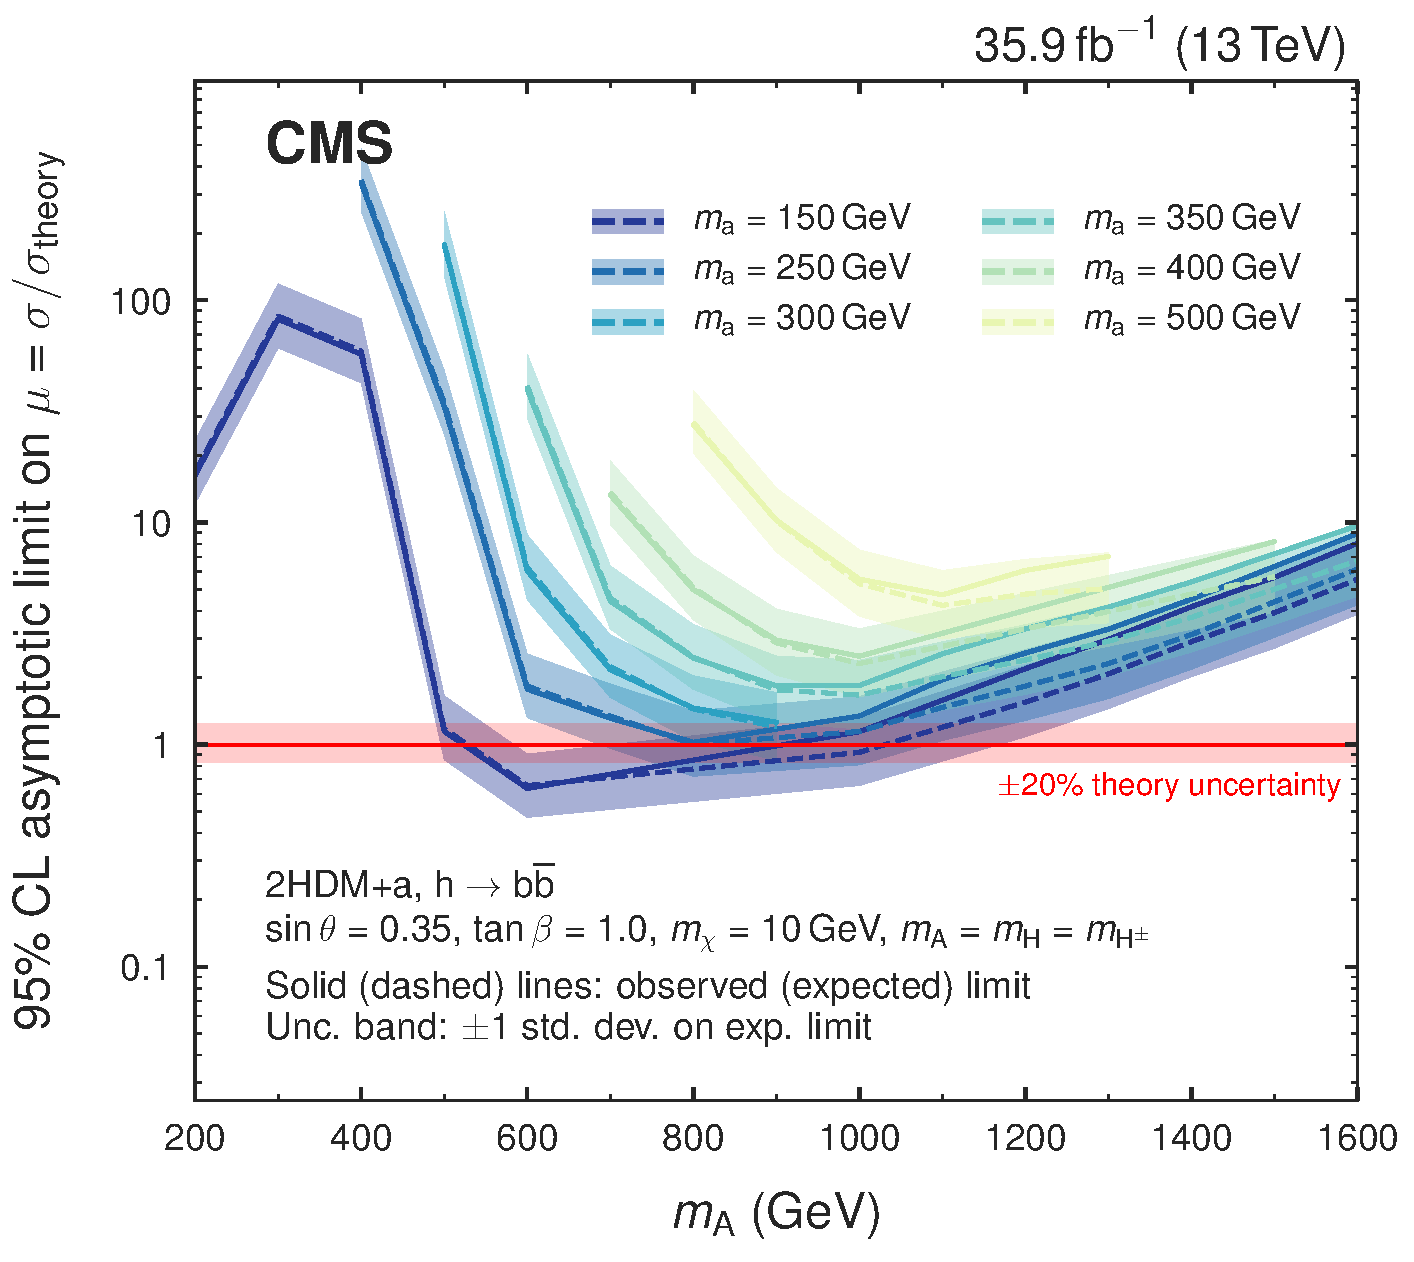
\includegraphics[width=0.475\textwidth]{figures/limits/limits_2hdma_mass.pdf}
  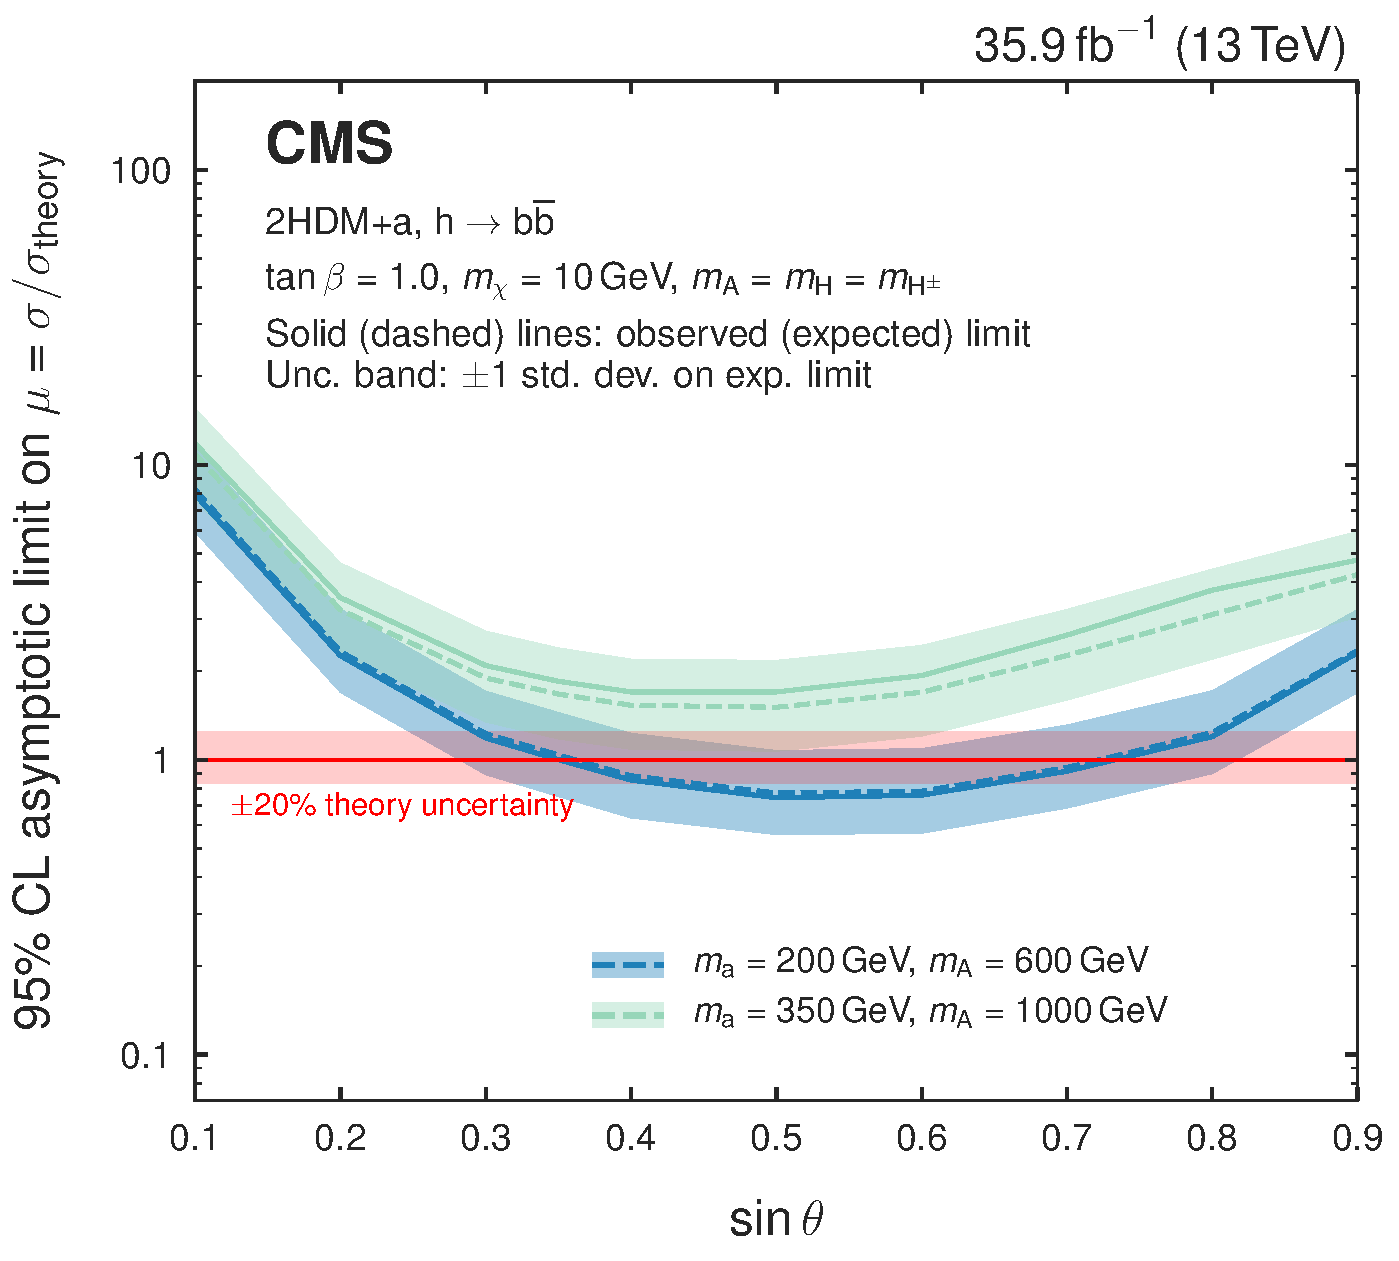
\includegraphics[width=0.475\textwidth]{figures/limits/limits_2hdma_sinp.pdf}\\
  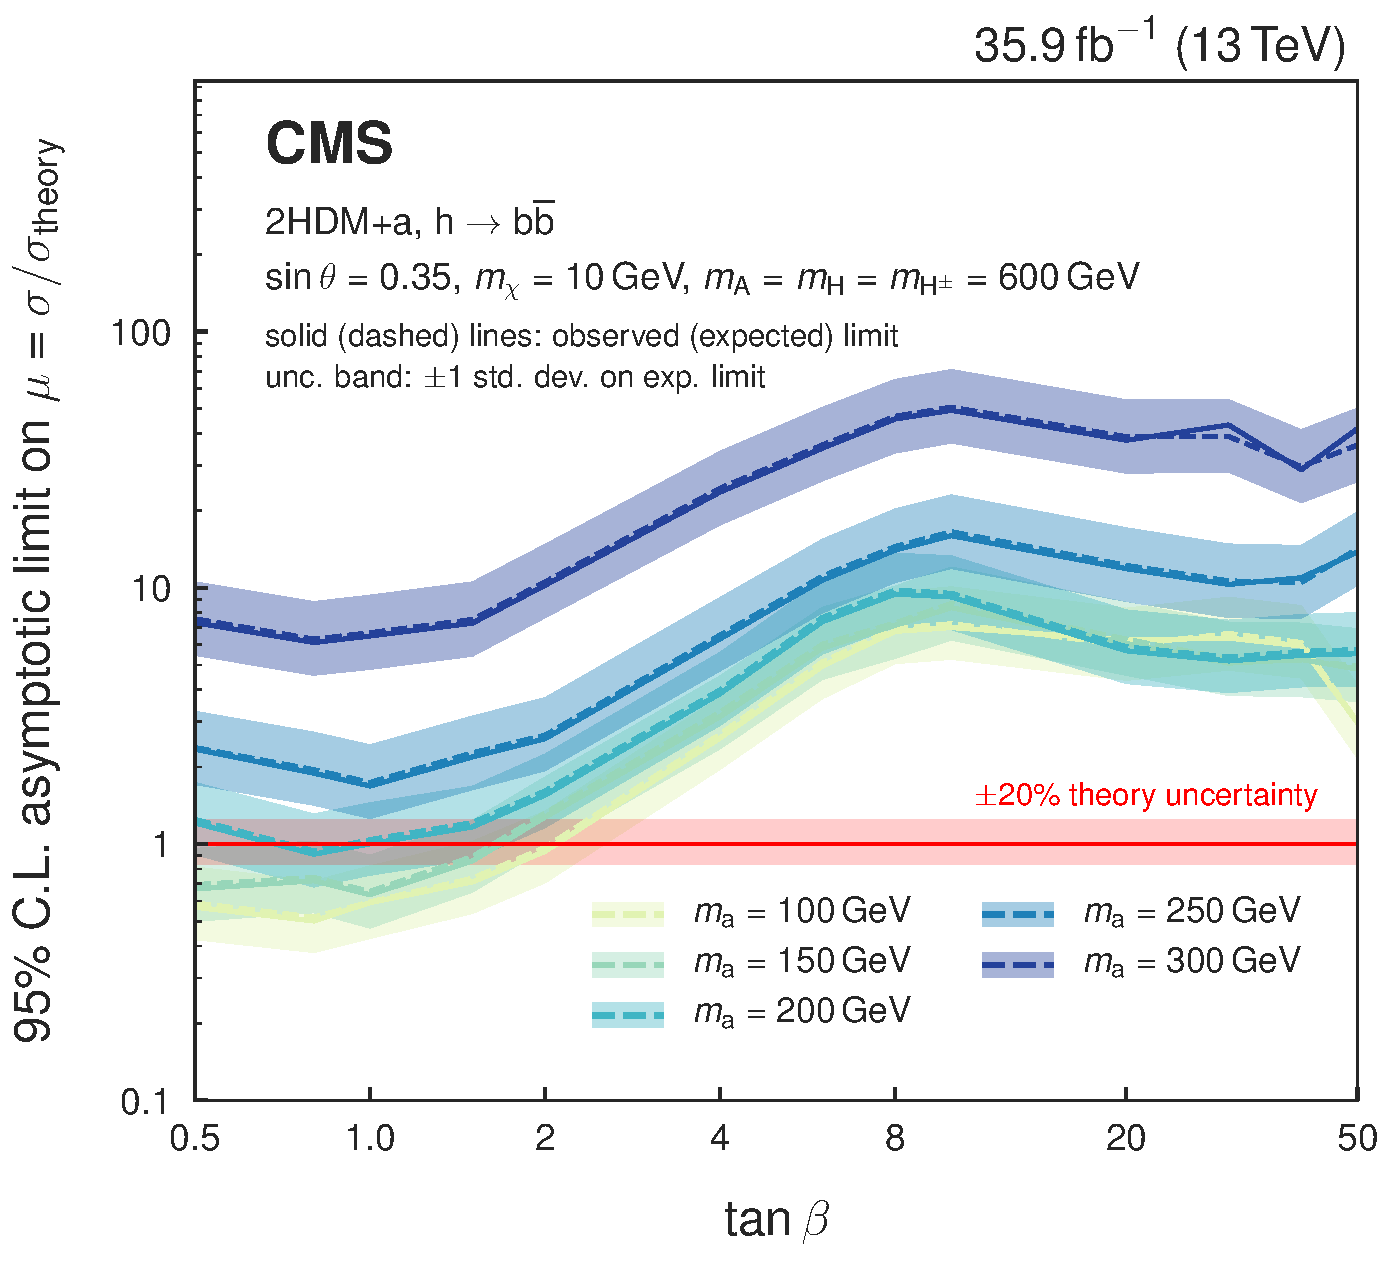
\includegraphics[width=0.475\textwidth]{figures/limits/limits_2hdma_tanb.pdf}\\
  \caption{Upper limits on the signal strength modifier for the 2HDM+$a$ model when scanning $m_\text{A}$ and $m_\text{a}$ (upper left), the mixing angle $\theta$ (upper right), or $\tan\beta$ (lower).}
  \label{fig:limits_2hdma}
\end{figure}


\begin{figure}[htbp]
  \centering
%  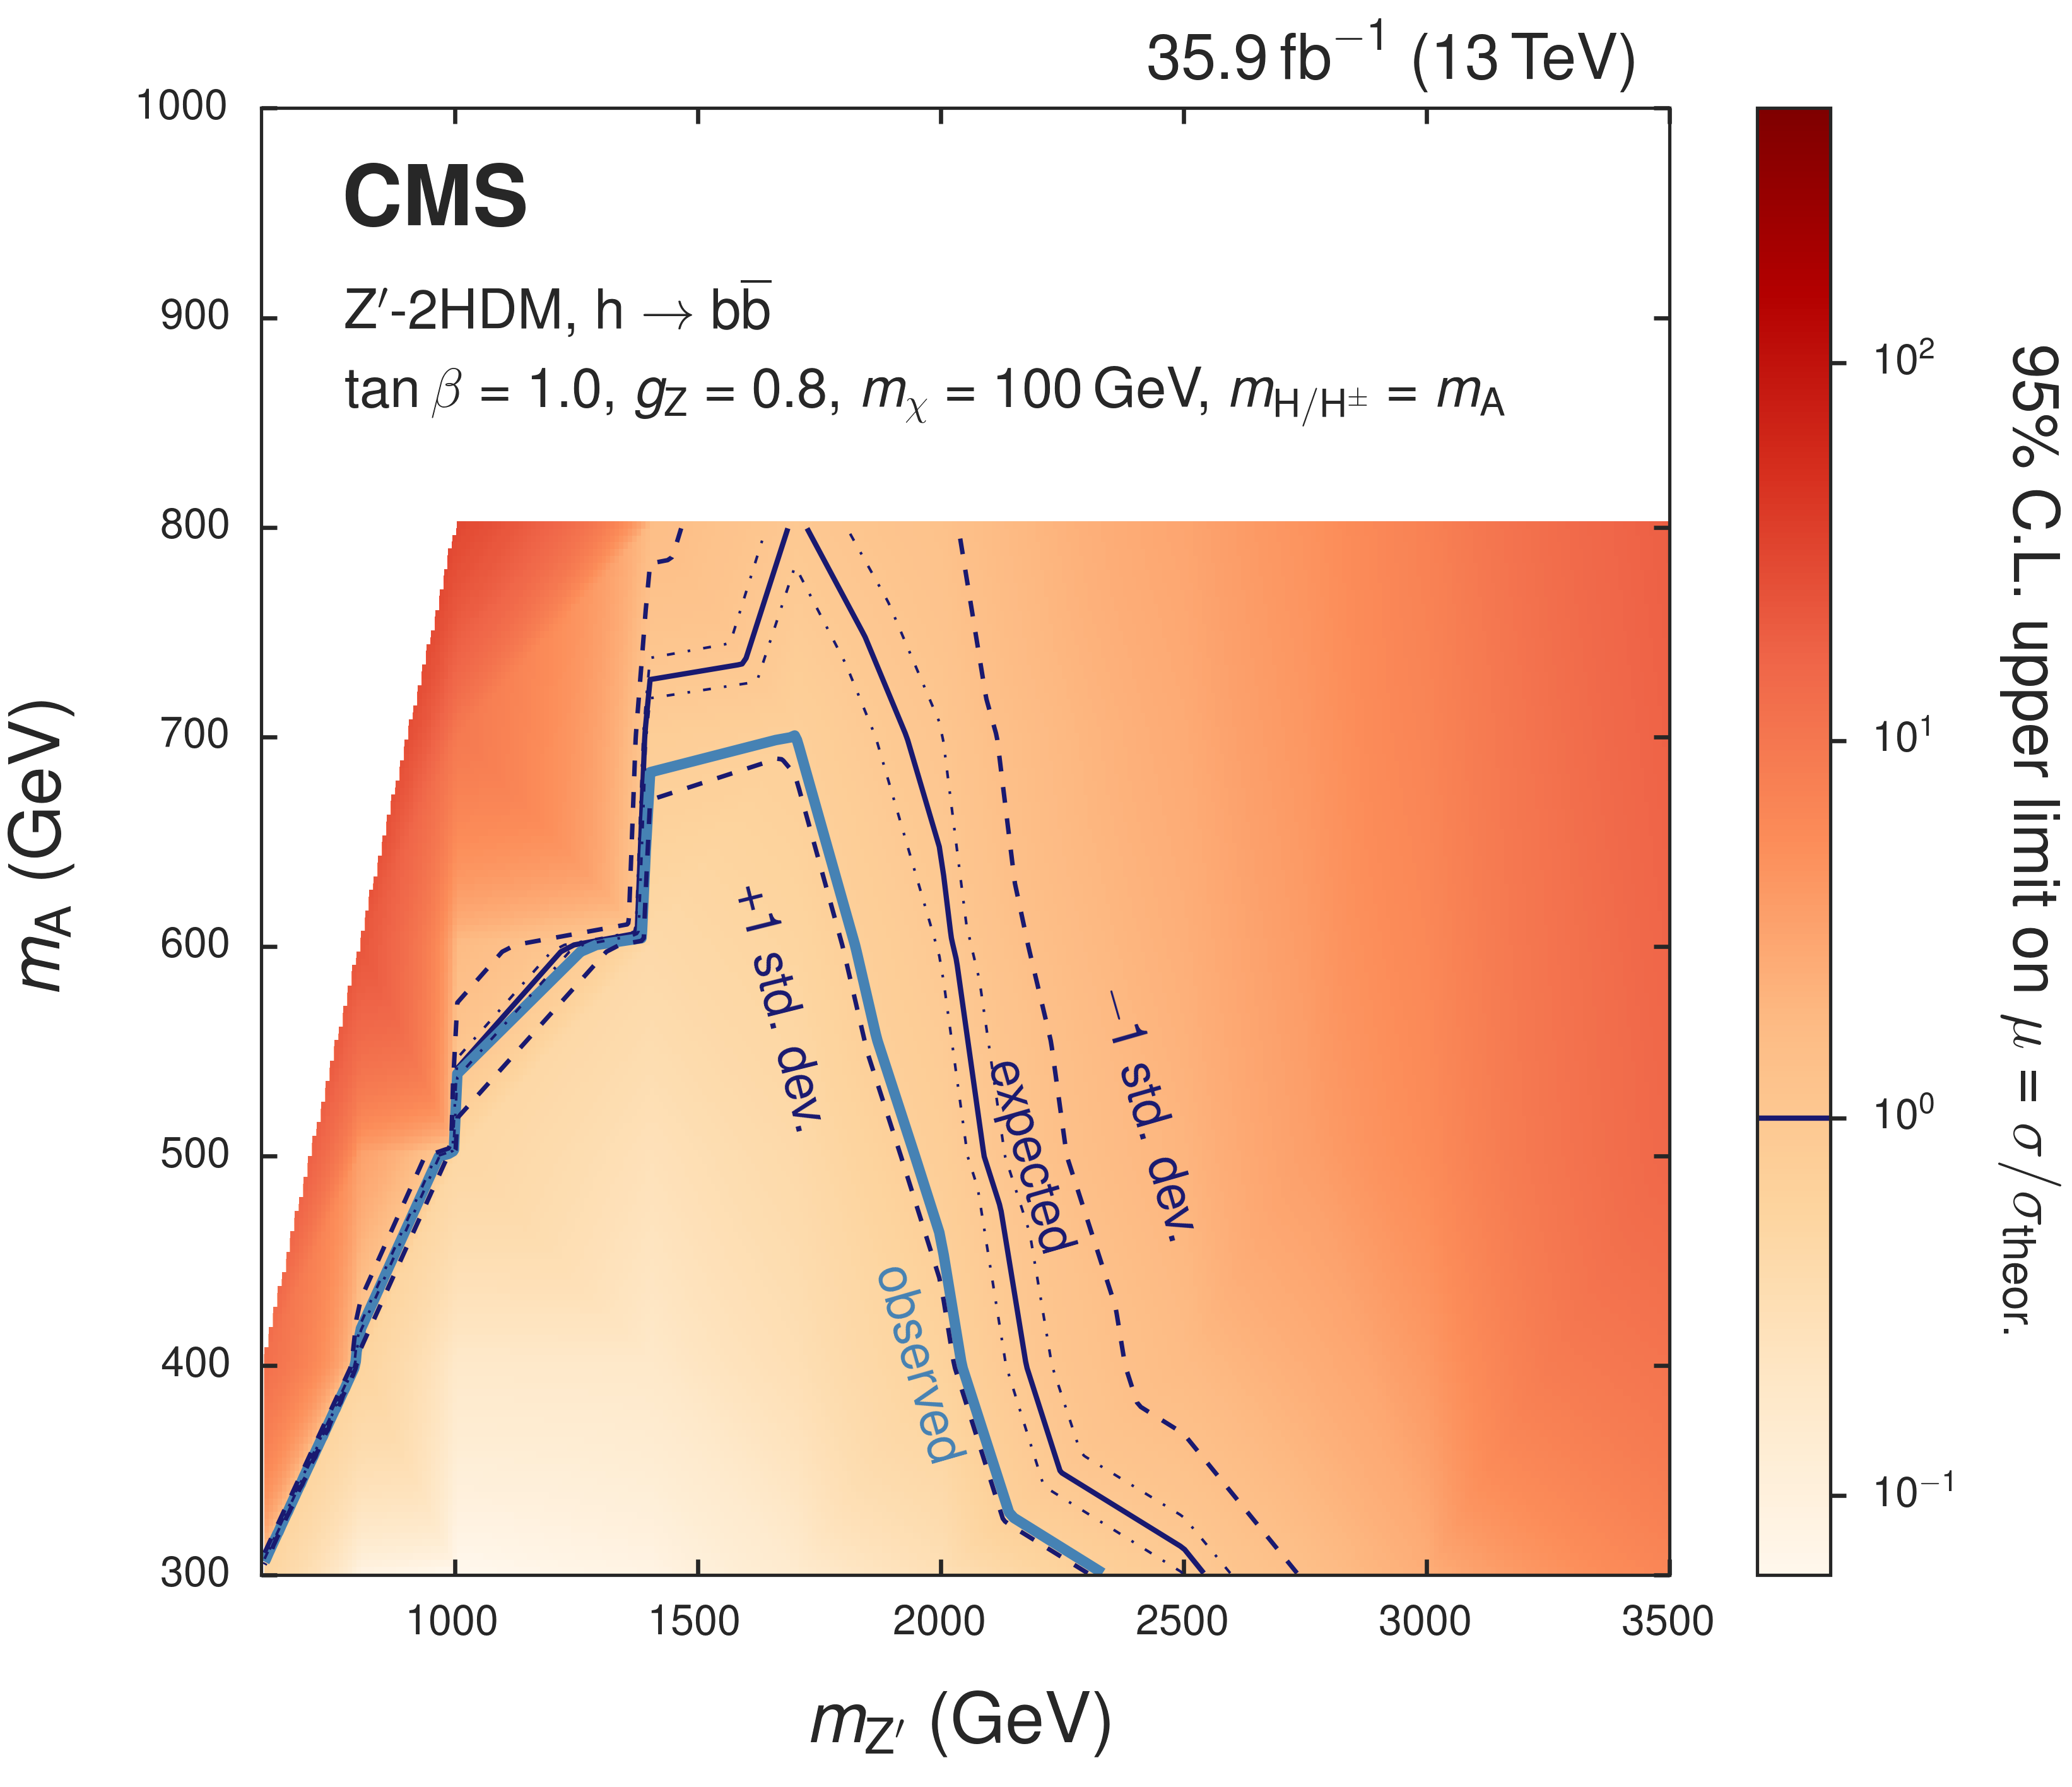
\includegraphics[width=0.475\textwidth]{figures/limits/limits_2hdm2d.png}
%  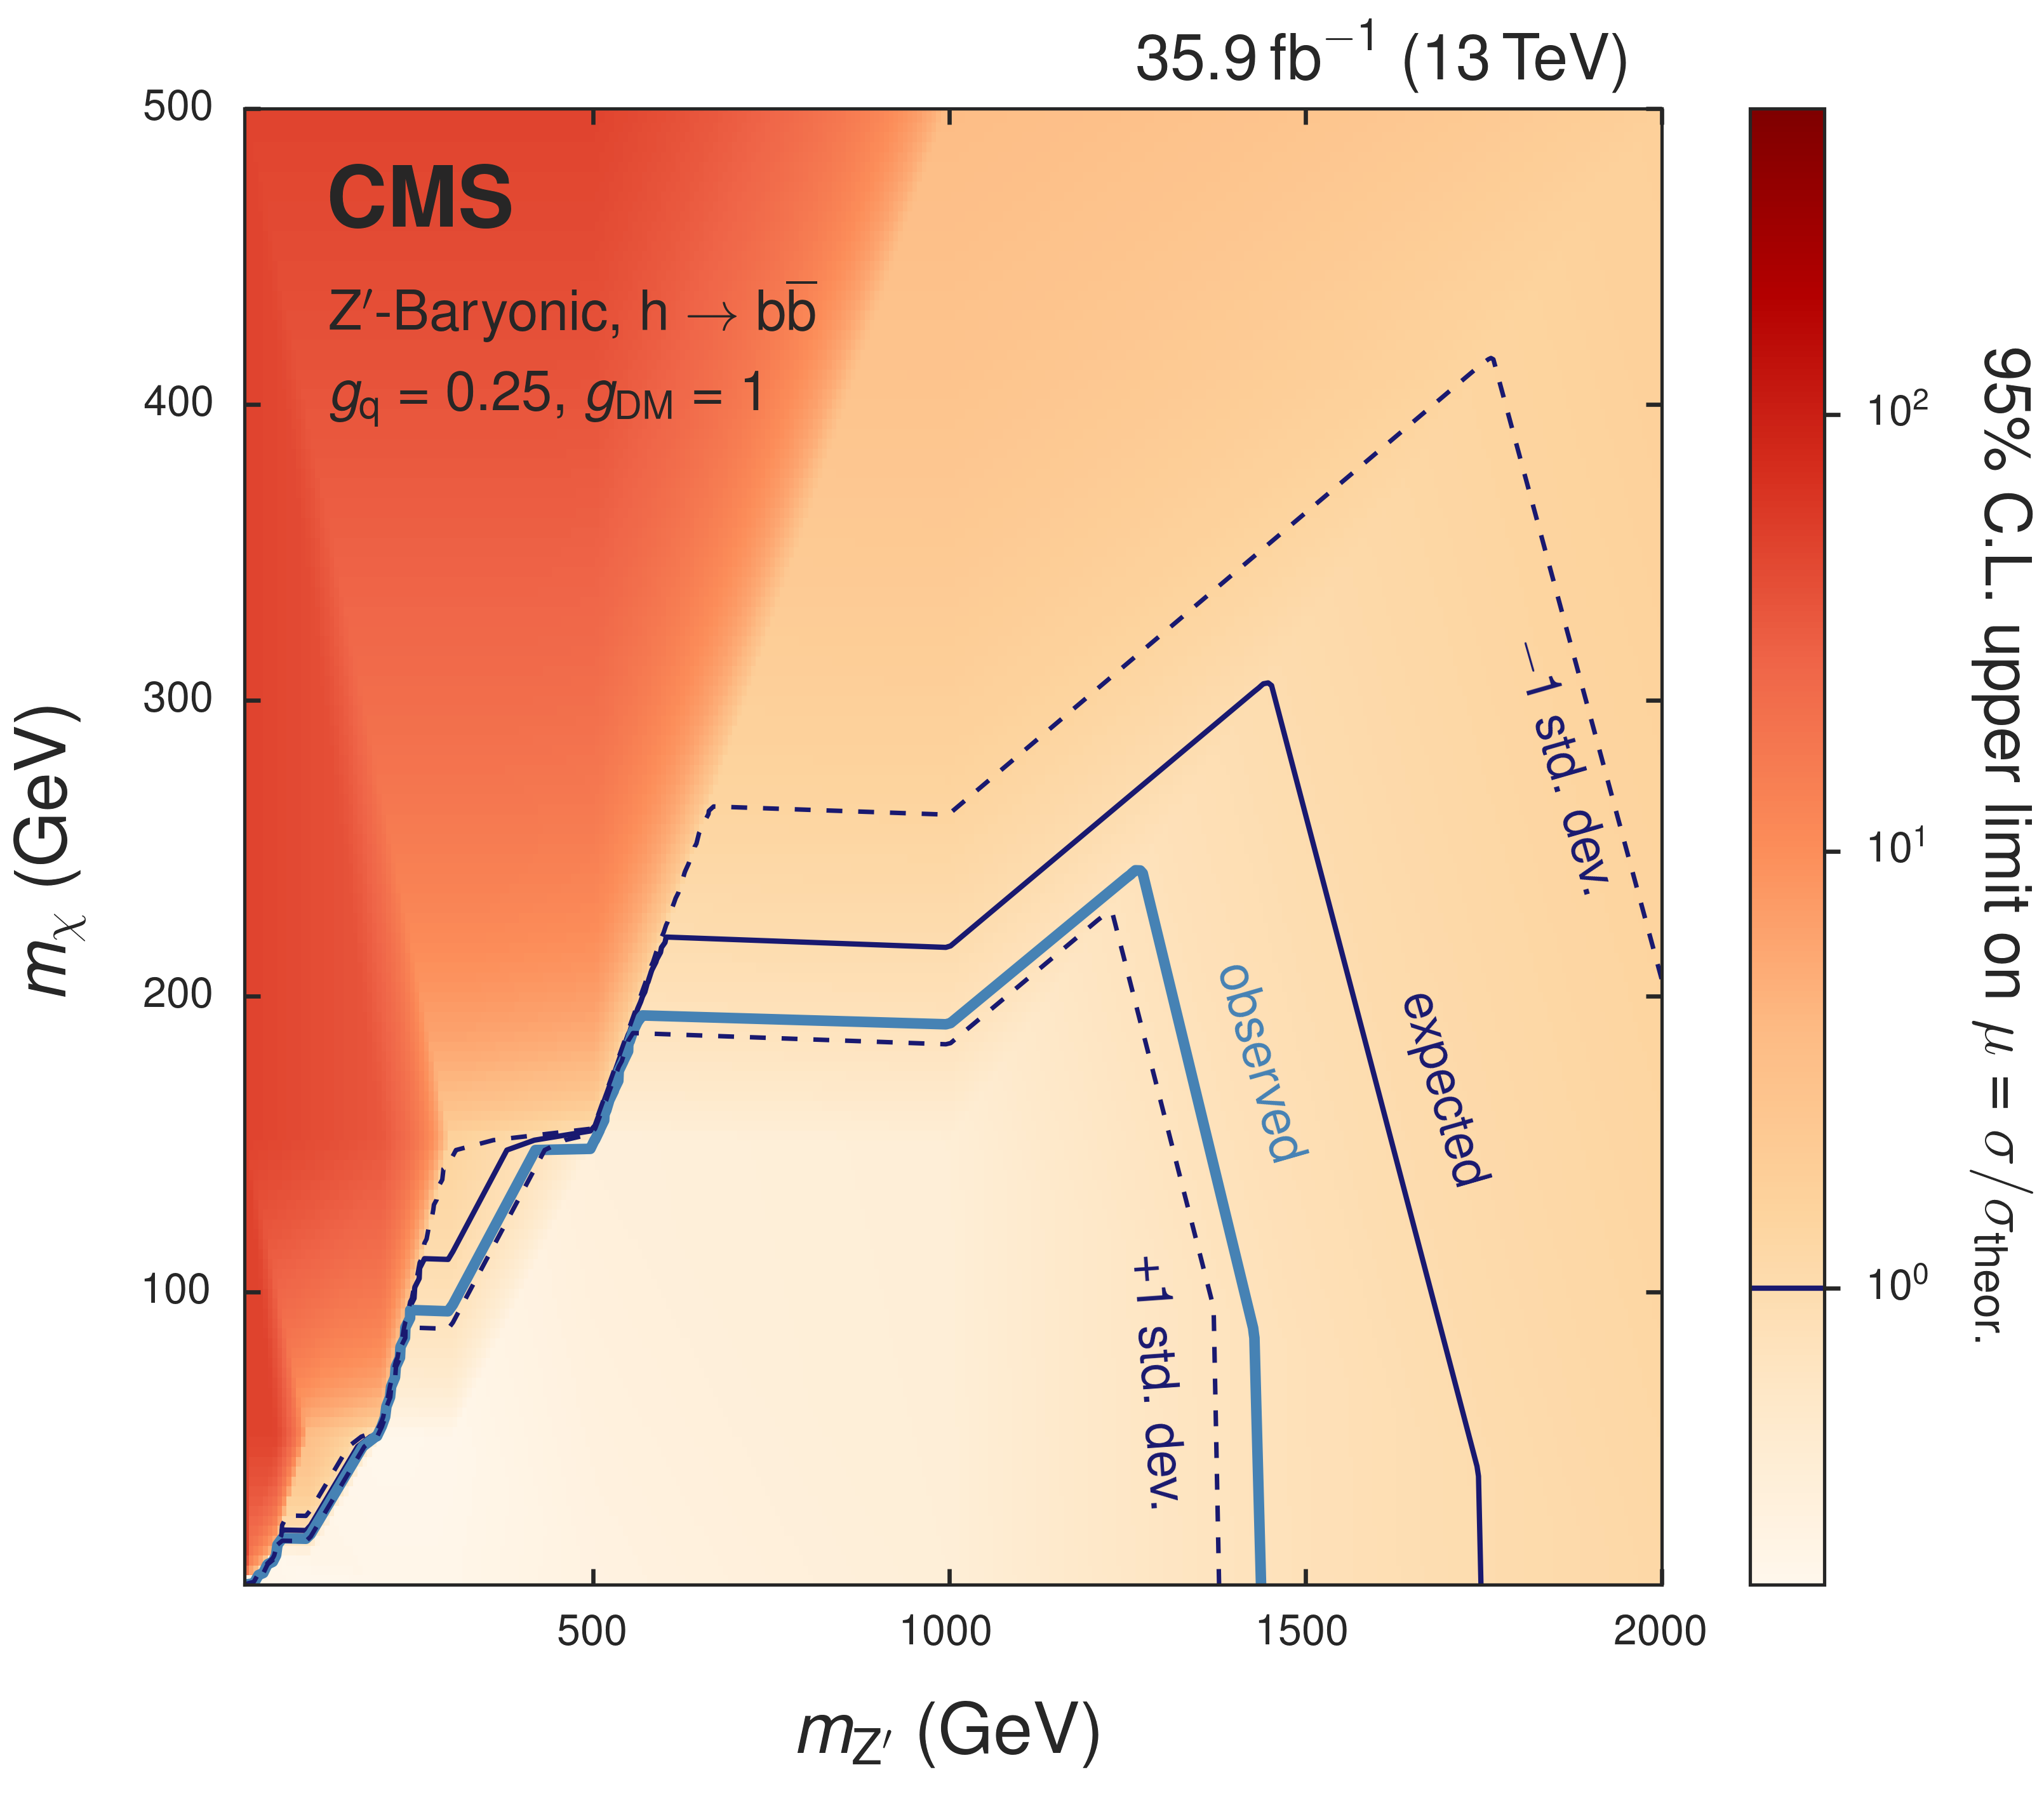
\includegraphics[width=0.475\textwidth]{figures/limits/limits_barzp2d.png}
  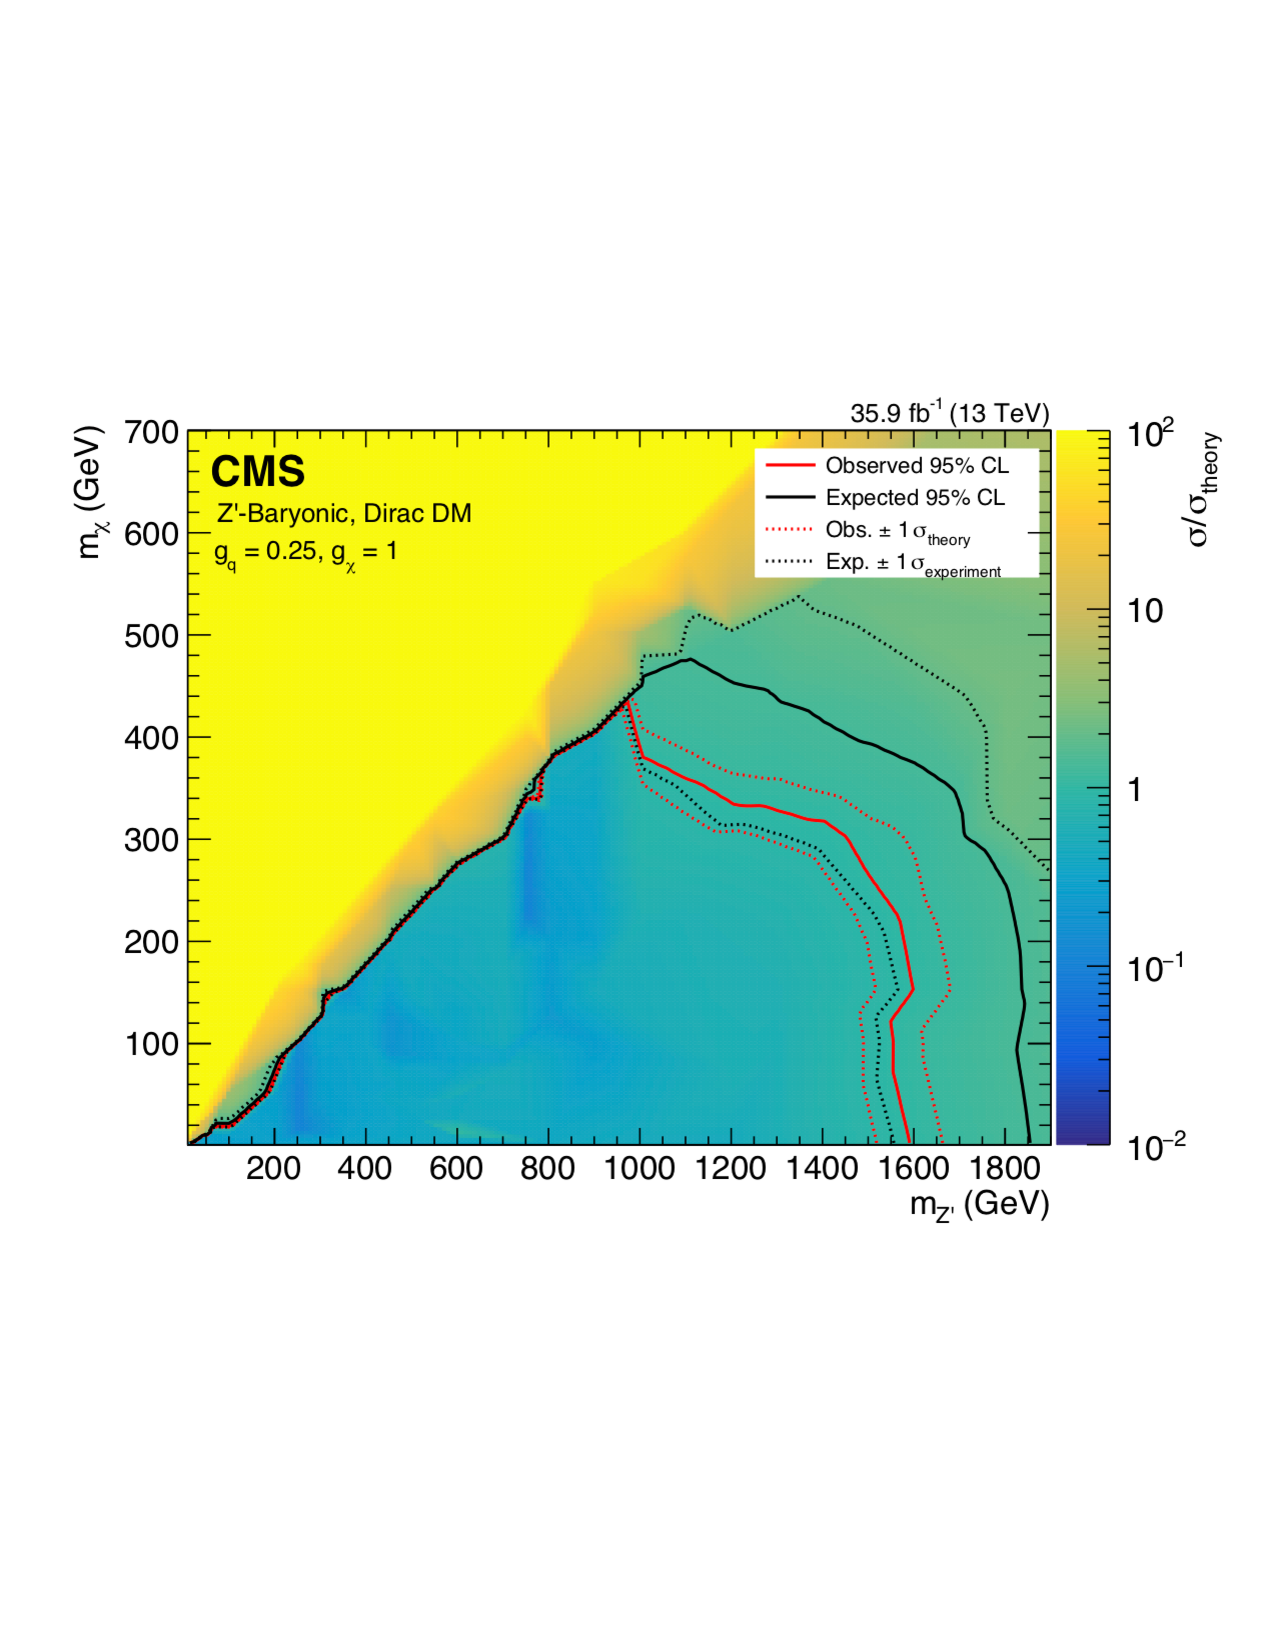
\includegraphics[width=0.475\textwidth]{figures/limits/limit2d_zpb_monohbb_.pdf}
  \caption{Upper limits on the signal strength modifier for the baryonic Z' model  as a function of $m_{Z'}$ and $m_\chi$. Mediators of up to 1.6\TeV are excluded for a DM mass of 1\GeV. Masses of the DM particle itself are excluded up to 430\GeV for a Z' mass of 1.25\TeV.}
  \label{fig:limits}
\end{figure}




Figure~\ref{fig:limits} shows the expected and observed exclusion range as a function of $m_{\text{Z}'}$ and $m_{\chi}$ for the baryonic Z' model. For a DM mass of 1\GeV, masses $\mzp<1.6\TeV$ are excluded. The expected exclusion boundary is 1.85\TeV. Masses for the DM particles of up to 430\GeV are excluded for a 1.1\TeV Z' mass. These are the most stringent limits on this model so far. %These results can be turned into limits on the spin-independent cross section, see $-$FIG XX$-$. 

To compare results with DM direct detection experiments, limits from the baryonic Z' model are presented in terms of a spin-independent (SI) cross section \SigSI for DM scattering off a nucleus.
Following the recommendation of Ref.~\cite{presentDM}, the value of $\sigma_\text{SI}$ is determined by the equation:

\begin{equation}
\sigma_\text{SI} = \frac{f^2(g_{\cPq})g^2_{\mathrm{DM}}\mu^2_{\mathrm{n}\chi}}{\pi m^4_{\mathrm{med}}},
\end{equation}

where $\mu_{\mathrm{n}\chi}$ is the reduced mass of the DM-nucleon system, $f(g_{\cPq})$ is the mediator-nucleon coupling, which is dependent on the mediator coupling to SM quarks $g_{\cPq}$, $g_{DM}$ is the mediator coupling to SM particles, and $m_{\text{med}}$ is the mass of the mediator.
The resulting \SigSI limits as a function of DM the mass are shown in Fig.~\ref{fig:limitsdd}.
%Exclusions from several direct detection experiments are compared to our result.
Under the assumptions made for the baryonic Z' model, these limits are the most stringent to date for $m_\chi < 5\GeV$.


\begin{figure}
  \centering
%  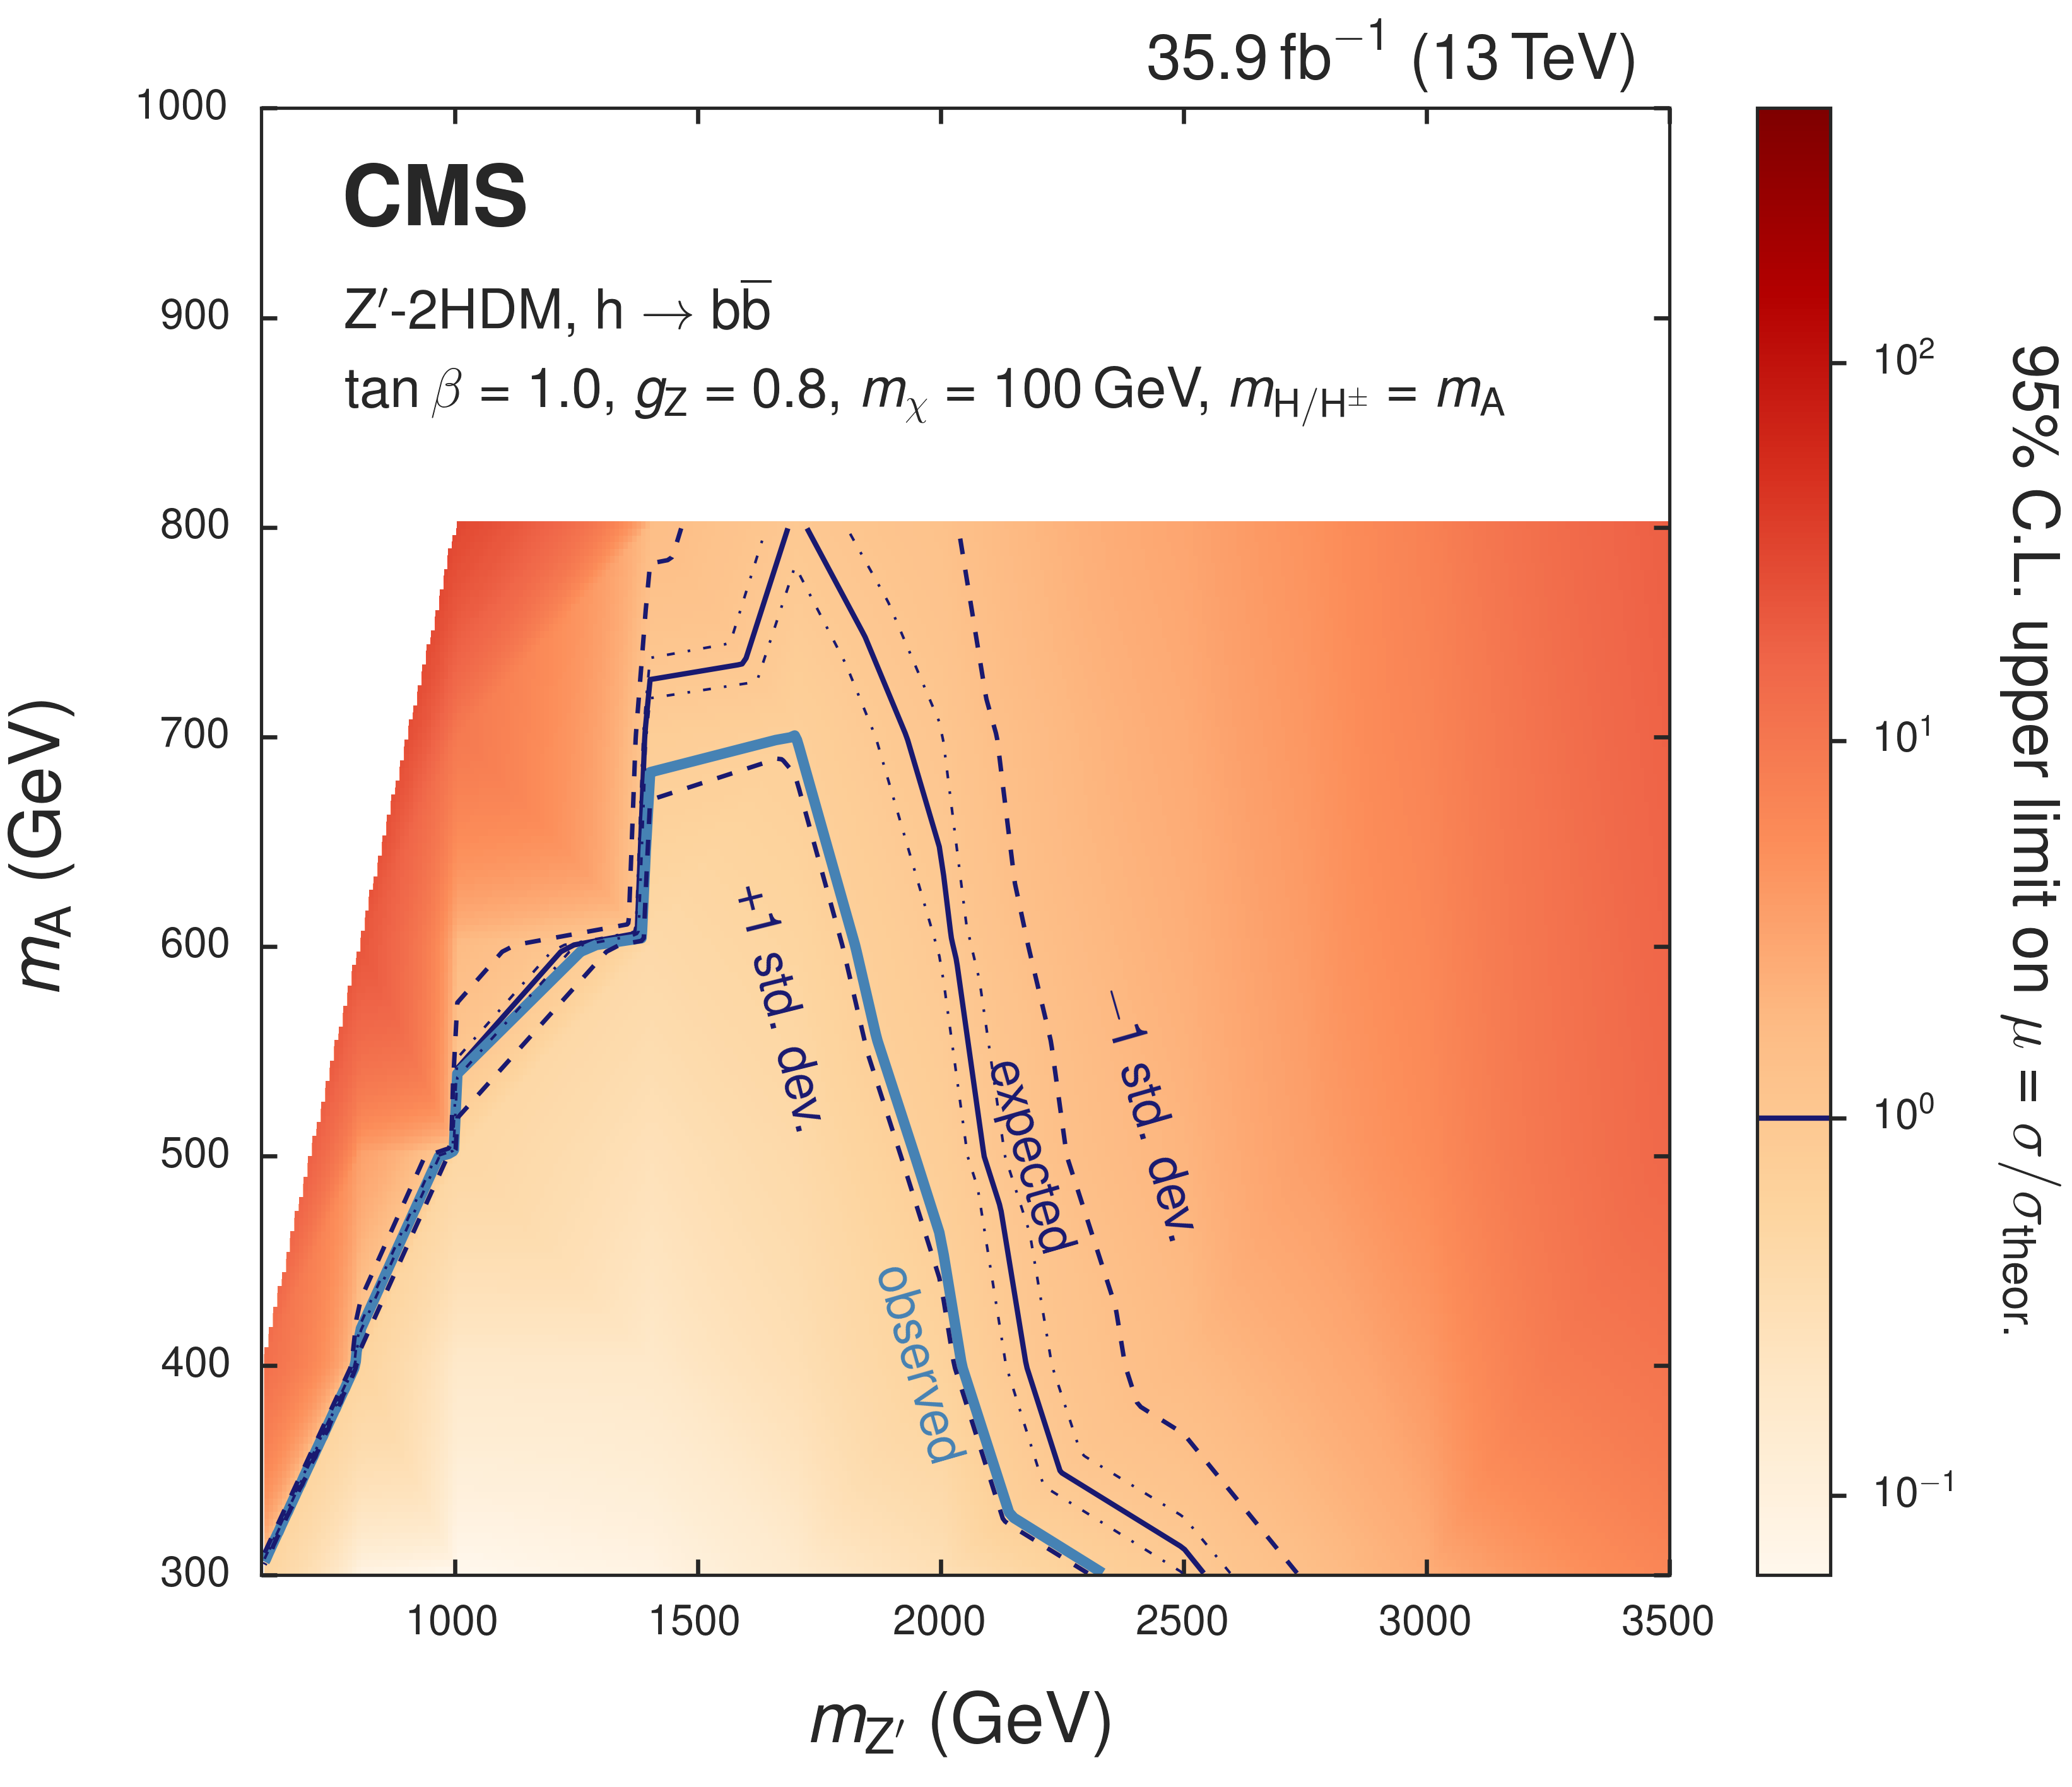
\includegraphics[width=0.475\textwidth]{figures/limits/limits_2hdm2d.png}
%  \includegraphics[width=0.475\textwidth]{figures/limits/limits_barzp2d.png}
  \includegraphics[width=0.775\textwidth]{figures/limits/SpinIndepend_XsecDM_MonoHbb_bb_obs_Summary.pdf}
  \caption{The 90\% \CL exclusion limits on the DM-nucleon SI scattering cross section as a function of $m_{\chi}$. 
Results on the baryonic Z' model obtained in this analysis are compared with those from a selection of direct detection (DD) experiments. 
The latter exclude the regions above the curves. 
Limits from CDMSLite~\cite{CDMSLite}, LUX~\cite{LUX}, XENON-1T~\cite{XENON1T}, PandaX-II~\cite{PandaxII}, and CRESST-II~\cite{CresstII} are shown.}
  \label{fig:limitsdd}
\end{figure}


\section{Summary}

A search for the associated production of dark matter (DM) particles with a Higgs
boson decaying into a pair of bottom quarks is presented. No significant
deviation from the predictions of the standard model (SM) is observed, and upper limits on
the production cross section predicted by a type-2 two Higgs doublet model
extended by an additional light pseudoscalar boson $a$ (2HDM+$a$) and the
baryonic Z' model are established. They constitute the most stringent collider exclusions placed on the parameters in these
models so far. For the nominal choice of the mixing angle $\sin\theta$
and $\tan\beta$ in the 2HDM+$a$ model, the search excludes masses
$500<m_A<900\GeV$ (where $A$ is the heavy pseudoscalar boson) assuming $m_a=150\GeV$. Scanning over
$\sin\theta$ with $\tan\beta$ = 1, we exclude
$0.35<\sin\theta<0.75$ for $m_\text{A}=600\GeV$ and
$m_\text{a}=200\GeV$.  Finally, $\tan\beta$ values between 0.5 and 2.0
(1.6) are excluded for $m_\text{A}=600\GeV$ and $m_\text{a}=100$
(150)\GeV and $\sin\theta$ $>$ 0.35. In all 2HDM+$a$ interpretations, a DM mass of $m_\chi=10\GeV$ is assumed. For the baryonic Z' model, we exclude Z' boson masses up to 1.6\TeV for a DM mass of 1\GeV, and DM masses up to 430\GeV for a Z' boson mass of 1.1\TeV. The reinterpretation of the results for the baryonic Z' model in terms of an SI nucleon scattering cross section yields a higher sensitivity for $m_\chi<5\GeV$ than existing results from direct detection experiments, under the assumptions imposed by the model. The 2HDM+$a$ model is probed experimentally for the first time.

 



%% **DO NOT REMOVE BIBLIOGRAPHY**
\bibliography{auto_generated}   % will be created by the tdr script.

%% examples of appendices. **DO NOT PUT \end{document} at the end
%\clearpage
\appendix
